
\documentclass[hyperpdf,bindnopdf,10pt]{hepthesis}

\usepackage[utf8]{inputenc}
\usepackage{graphicx}
\usepackage{tikz} 
\usepackage{bbold}
\usetikzlibrary{shapes,arrows,positioning,automata,backgrounds,calc,er,patterns}
\usepackage{tikz-feynman}
\tikzfeynmanset{compat=1.0.0}
\usepackage{breqn}
\usepackage{enumitem}
\usepackage{dsfont}
\usepackage{amsmath}
\usepackage{subfig}



\graphicspath{{images/}}

\newcommand{\SUN}{{\mathrm{SU}(N)}}
\newcommand{\MET}{{$E_{T}^{miss}$ }}
\newcommand{\Hgg}{{$\mathrm{H}\rightarrow{\gamma\gamma}$ }}
\newcommand{\Zee}{{$\mathrm{Z}\rightarrow{\mathrm{e}^{+}\mathrm{e}^{-}}$ }}
\newcommand{\Zmumu}{{$\mathrm{Z}\rightarrow{\mu^{+}\mu^{-}}$ }}
\newcommand{\ttH}{{$\mathrm{t}\bar{\mathrm{t}}\mathrm{H}$ }}


\title{Study of Higgs boson production through vector boson fusion at the CMS experiment using a dense convolutional neural network}
\author{Jack Charles Wright}

\begin{document}

\begin{frontmatter}
    

\chapter*{\centering Abstract}
Measurements of the Higgs boson using the \Hgg Higgs boson decay mode and two different methods for identifying Higgs bosons produced via vector boson fusion are presented.
These analyses use proton-proton collision data collected by the CMS collaboration during the 2016 running period and constitute 35.9\,fb$^{-1}$ of integrated luminosity at $\sqrt{s}=13$\,TeV.
One vector boson fusion identification method is based on boosted decision trees, and the other is based on jets formulated as images and a dense convolutional neural network. 
The categorisations produced by both methods are subjected to the overall \Hgg statistical analysis and their results compared.
The neural network itself is also subjected to analysis to determine what features it has learned to extract from the jet images.

The main objectives of this new approach are to reduce contamination from gluon fusion in the vector boson fusion categories and to improve their statistical significance. 
This is indeed observed in the expected yields measured from simulation.
The vector boson fusion signal strength relative to the Standard Model is measured to be $0.8^{+0.6}_{-0.5}$ in the boosted decision tree variant and $1.5^{+0.5}_{-0.5}$ in the neural network variant. 
The neural network is also observed to give a reduced uncertainty on many of the other measurements, especially those more directly impacted by vector boson fusion production.


\chapter*{\centering }% Dedication}
\begin{center}
    \thispagestyle{empty}
    To Mum and Dad. \\
    I'm sorry about the electricity bill.
\end{center}


\chapter*{\centering Declaration}
I declare that this thesis is my own work. It has been built upon the work of others and this is stated in detail below. 
When the work of others is used in the text it is referenced appropriately.

\textbf{Chapter 1} introduces the work in this thesis referencing prior results in the fields of particle physics and machine learning in my own words.

\textbf{Chapter 2} describes particle physics theory that has been entirely developed by others, but in my own words.

\textbf{Chapter 3} describes the Large Hadron Collider and Compact Muon Solenoid in my own words, but these again were developed and studied by many experimental physicists before me.

\textbf{Chapter 4} describes machine learning theory and practise. This is covers the work of various individuals in the field with my own words.

\textbf{Chapter 5} describes physics objects at CMS. I had a role in part of the calibration of the ECAL for energy scales and smearing. The systems and studies are the work of my other colleagues at CMS.

\textbf{Chapter 6} describes event categorisation. The vector boson fusion tagging is the focus of my work and is based on the official analysis approach. I developed the current version of the boosted decision tree based vector boson fusion tag along with Dr Yacine Haddad. The neural network based vector boson fusion tag is my own work. The other tags are the work of other members the CMS \Hgg analysis group.

\textbf{Chapter 7} describes the final statistical analysis. The official results are the work of the entire \Hgg analysis group. For the neural network based results I developed a framework to produce information in a format that could be consumed by the existing final fits machinery. The final fits over the neural network variant categories were run by Ed Scott.  

\textbf{Chapter 8} summarises and draws conclusions. This is my own writing, and the future developments are my own suggestions.

\begin{flushright}
    Jack Charles Wright
\end{flushright}

\chapter*{\centering Acknowledgements}
This thesis depends on the contributions of many more people than I can name here. 
I will always be thankful for the last four years and all the good people I've had the privilege to meet and work with.
Therefore I'd like to express my sincere gratitude to everyone I'm about to neglect. 

To begin with I'd like to thank Imperial College London and the HEP group for giving me this opportunity in the first place, and STFC for providing funding.
I'd also like to thank CERN, the LHC and the CMS collaboration for building and running such remarkable machines and for providing a great environment for research.
I am particularly grateful to the Max Planck Institute for Intelligent Systems for accepting me into MLSS 2017 and providing such an enriching two weeks that taught me so much. 

A special thank you must go to my supervisors Prof Paul Dauncey and Dr Chris Seez for their support and deep expertise.
Thank you Chris for welcoming me to CERN and your uncompromising honesty, and thank you to Paul for making so much time for me and being so supportive even though you're head of group. I couldn't have asked for anyone better.

I am grateful for my colleagues Dr Seth Zenz, Dr Yacine Haddad and Ed Scott. 
Seth, without your tireless hard work and dedication I and many others would be up the proverbial creek with no paddle.
Yacine, your encouragement and permanently sunny disposition helped me so much. Both of you have taught me a lot. 
Finally, special thanks to Ed for your help over the past couple of years but especially for all your work with the final fits. 
I wish you the best of luck as you start your thesis, I sincerely hope it goes a lot smoother than mine. 

Thank you to Daniel Saunders and his partner Elliot for helping me at an especially difficult time.
I wish you both the very best for your future together.

I am also grateful for the deep kindness and generosity of the Paslay family. 
I'll never forget what you've done for me over the years. 

I am eternally thankful to my amazing partner Lucie Altenburg for all the love and support she has shown me over the last year. 
You've helped me back up when it all seemed to be going to bits, you've proofread for me and more. 
I can't begin to thank you enough for how you've looked after me. 

Finally, none of this would have been possible without the love and warmth of my family: you're all the bedrock of my life.
Above all I'd like to thank my wonderful parents Maureen and Kevin Wright who have shown me unwavering support and fed my curiosity from a the start.
I fondly remember childhood visits to the old Birmingham science museum where we'd look all the machines, at the wave motion and light spectrum displays.
I especially remember the boxes with table top physics experiments we used to do with prisms, bridge building and other things. 
You gave me all the books I could ever want on all the subjects I was interested in and then some. 
You've done so much more for me than I could ever express in here, and this thesis is a culmination of all of that. 
I feel this is your achievement as well as mine. 

\tableofcontents
\listoffigures
\listoftables
%
\chapter*{\centering }
\begin{center}
\epigraph{\textit{``ALL THIS IS A DREAM. Still, examine it by a few experiments.''}}{Michael Faraday\\ Laboratory journal entry \#10040}
\end{center}

\cleardoublepage

\end{frontmatter}


\begin{mainmatter}

    \cleardoublepage

    \chapter{Introduction}
\label{chap:intro}

%\newpage
The Standard Model (SM) of particle physics has had its remarkable predictive power demonstrated through many experimental confirmations. 
At the core of this success is the Higgs field and the way its behaviour radically alters the phenomenology of a pristine, symmetric and massless theory.

The SM consists of a collection of fields whose quanta constitute fundamental matter particles and force mediators, as well as the couplings between them. 
These couplings determine the interactions in particle physics processes: the signals we observe in experiment. 
All of these particles, and many of their interactions, have been discovered by generations of high-energy particle physics experiments. 
This culminated in the completion of the field content of the SM with discovery of the Higgs boson itself in 2012 by the ATLAS and CMS collaborations~\cite{ATLAS_Higgs_disc,CMS_Higgs_disc}. 

It is also known that the SM gives an incomplete description of nature. 
There is no dark matter candidate to explain experimental observations such as the bullet cluster~\cite{BulletCluster}, there is no description of the force of gravity, 
and neutrinos are considered massless when they are known not to be~\cite{NeutrinoOscillation}. 
Various extensions to the SM have been suggested~\cite{BSM}, and these can manifest as entirely new particles and as deviations in SM-expected rates for some processes. 

This raises the question of precisely what sort of Higgs boson has been discovered. How does the Higgs field grant mass to the fermions? 
How does it self-interact and what is the shape of the potential it experiences? Are there any unexpected couplings that alter the Higgs boson's production and decay?
As we enter the precision measurement era of Higgs physics we aim to answer these questions, and hopefully shed light on physics beyond the SM.
\\

Precision measurement depends on high-quality data and superior signal extraction.
The field of machine learning (ML) has produced many algorithms that are used throughout experimental particle physics in both detector operation and data analysis. 
The discovery of the Higgs boson decaying to a diphoton system (\Hgg) in particular used these techniques in concert with its characteristically clean signal. 
Here signal extraction is enhanced using information from extra objects characteristic of certain predicted Higgs production modes and an algorithm called a boosted decision tree (BDT). 

BDTs have been a reliable workhorse of particle physics for over a decade~\cite{MiniBooneBDT}, but ML has made exceptional leaps in recent years thanks to deep learning (DL).
In particular, DL applied to image recognition has resulted in powerful approaches that achieve super-human performance~\cite{ResNet}. 
This thesis explores how to use these techniques to improve the extraction of \Hgg events produced via Vector Boson Fusion (VBF). 
Specifically, VBF signal extraction is reformulated in part as an image classification problem where VBF's characteristic jets of particles are treated as images.  
\\

This thesis is based on the 2016 \Hgg analysis~\cite{HIG-16-040}, and is structured as follows: Chapter~\ref{chap:theory} begins by describing the theory underlying the SM, then the SM itself with emphasis on the Higgs sector and its phenomenology. 

Chapter~\ref{chap:apparatus} describes the experimental apparatus used to produce and record the proton collision dataset used in this thesis: the Large Hadron Collider (LHC) and the Compact Muon Solenoid (CMS). CMS is described in detail with each detector subsystem's structure and operation explained with emphasis on the electromagnetic calorimeter.

Chapter~\ref{chap:machine_learning} presents an introduction to machine learning covering basic theory, how to control model capacity for generalisation performance, ensembles (BDTs), plus how to design and tune an ML algorithm. The chapter then introduces neural networks and deep learning, culminating in the more advanced dense convolutional neural network (DCNN) models used in this thesis. 

Chapter~\ref{chap:object_reco} describes how physics objects are reconstructed at CMS with emphasis on photons and how they are formed into \Hgg diphoton candidates.

Chapter~\ref{chap:event_select} describes how candidate \Hgg events are categorised by different tags in the analysis for signal enhancement.  
Each of the tags is described in turn, but VBF will be described and validated in fine detail in both the BDT-based and DCNN-based variants. 
The DCNN will also be examined to determine what features it has learned to detect using a collection of network interpretation techniques.

Chapter~\ref{chap:statistical} describes the final statistical analysis of the categorised \Hgg candidates and the resulting measurements.
The construction of the statistical models for signal and background are described, and a full description of all of the systematic uncertainties is given. 
Final results of yields and likelihood scans of signal strength and coupling modifiers performed for analyses with the DCNN-based VBF tags and compared to the BDT-based results. 

Finally, Chapter~\ref{chap:conclusions} discusses the conclusions we may draw as well as possible avenues for future development and research. 






    \chapter{Theory}
\label{chap:theory}

%\chapterquote{The career of a young theoretical physicist consists of treating the harmonic oscillator in ever-increasing levels of abstraction.}{Sidney Coleman}

\newpage

\section{Introduction}
Modern particle theory is built upon the twin pillars of Yang-Mills theories and spontaneous symmetry breaking. 
Our best current model, the Standard Model (SM), is built from two such theories: electroweak theory and quantum chromodynamics. The former of these has its gauge symmetry spontaneously broken. 
In this chapter we will explore these two ideas before moving on to how they are used to construct the SM with particular emphasis on the mechanism of symmetry breaking and one of its phenomenological consequences: the Higgs boson. 

\section{Yang-Mills Theories}
\subsection{From Geometry to Gauge Fields}
The gauge covariant derivative $D_{\mu}$ and the field strength tensor $F_{\mu\nu}$ are two vital mathematical objects when one wants to construct the Lagrangian of a Yang-Mills theory.
Far from simply being an ansatz, they have a deep origin in the fundamental geometry of field theory. 
Their origin is outlined in this section: we start by describing the concept of a fibre bundle, its relationship to the internal symmetries of a field, and how the `warping' of a fibre bundle is related to the covariant derivative and the field strength tensor.

A fibre bundle $\mathcal{B}$ is a space which can be considered to consist of two parts: the base space $\mathcal{M}$ and the fibre $\mathcal{V}$. For each point $p$ in the base space there is an associated copy of the fibre space and these fibres do not intersect. 
In the context of a field one can consider these to be the external and internal spaces respectively. A special case is an ordinary product space where $\mathcal{B}$ is simply the Cartesian product of $\mathcal{M}$ and $\mathcal{V}$, generally one has more warped examples with curvature and less trivial topology. A visual example is given in Figure \ref{fig:theory:fibre_bundle}.
\begin{figure}[h!]
    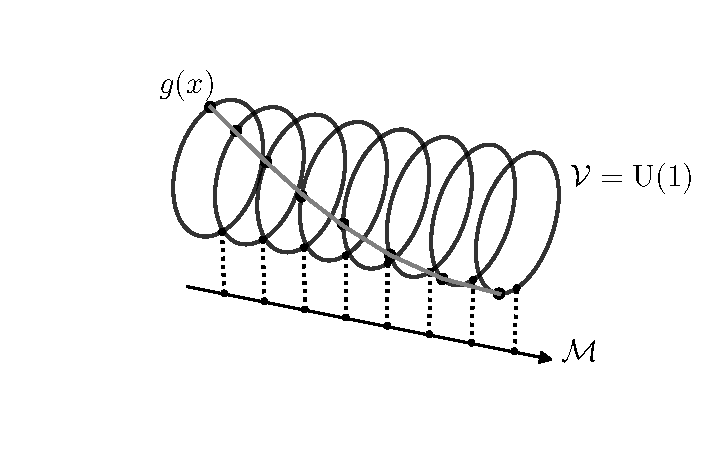
\includegraphics[width=0.5\textwidth]{figures/theory/fibre_bundle.pdf}
    \caption{A fibre bundle with $\mathcal{V} = \mathrm{U}(1)$. A section is shown (grey line) choosing $g(x)\in\mathrm{U}(1)$ for a set of points in $\mathcal{M}$.}
    \label{fig:theory:fibre_bundle}
\end{figure}
These warped examples are of interest in gauge theory, specifically when there is curvature in the fibre space with no torsion.

Particularly, we are interested in the cases when $\mathcal{V}$ is symmetric under some Lie group $\mathcal{G}$ (in our case $\SUN$). 
These symmetries allow for the warping of the fibre bundle and correspond to the internal symmetries of a field. 
Furthermore, one can model these examples by taking the fibre to be $\mathcal{G}$ with the identity element not at a fixed location. 
One can then `lift' the base space into the bundle: for each base space point we get a point within the associated fibre. In the gauge theory context choosing a section of the fibre bundle means choosing a particular $g(x)\in\mathcal{G}$, this is picking a gauge. 

To understand the warping of the fibre bundle we need the notion of a connection just like with the warped spaces of General Relativity.
This will allow for the introduction of warping to the internal space, and construction of invariants such as curvature and torsion tensors.
We can do this by constructing a differential operator $D_{\mu}$, and in our case of a fibre bundle with $\mathcal{V}=\mathcal{G}=\SUN$ where the internal space is simply stretched with no torsion we have,
\begin{equation}
\label{eq:theory:g_connection}
D_{\mu} = \partial_{\mu} - igA_{\mu}^{a} T^{a},
\end{equation}
where $A_{\mu}^{a}$ are generally complex-valued functions that depend on $x_{\mu}$ and operate by multiplying the input, and $T^{a}$ are the generators of the Lie group $\SUN$ which provide a basis in the fibre space with $a = 0,\ldots,N^{2}-1$.
We recognise this as having the familiar form of the gauge covariant derivative and the $A_{\mu}^{a}$ as the gauge potential. 

Now we have the connection we can begin to construct invariants of the geometry of the internal space. In particular we can construct the curvature tensor as follows
\begin{equation}
    \label{eq:theory:g_curvature}
    \frac{i}{g}[D_{\mu},D_{\nu}] = F_{\mu\nu} = \partial_{\mu} A^{b}_{\nu} T^{b} - \partial_{\nu} A^{a}_{\mu} T^{a} - ig[A^{a}_{\mu}T^{a}, A^{b}_{\nu}T^{b}].
\end{equation}
We recognise this form as the field strength tensor.

One can now see what occurs when a global symmetry is promoted to a gauge symmetry: we have induced some non-trivial warping of the field's internal space that gives rise to the $A^{a}_{\mu}$ gauge fields and their kinematics through the curvature $F_{\mu\nu}$.

\subsection{Constructing a Lagrangian}
With these ingredients we can construct a generic Yang-Mills Lagrangian with a straightforward procedure: we begin with a global symmetry of the fields that we promote to a gauge symmetry, we construct the gauge covariant derivative, replace $\partial_{\mu} \rightarrow D_{\mu}$ in the free theory, and add an interaction term based on the field strength tensor. 
As a concrete example, consider the collection of massive free Dirac fermions which we will turn into an interacting gauge theory with $\mathcal{G} = \SUN$.
We first construct the gauge covariant derivative, 
\begin{equation}
    \label{eq:theory:generic_SUN_Dmu}
    D_{\mu} = \partial_{\mu} - igA_{\mu}^{a} T^{a},
\end{equation}
and replace $\partial_{\mu} \rightarrow D_{\mu}$ in the free Lagrangian
\begin{equation}
    \label{eq:theory:int_dirac_no_gauge_dynamics}
    \mathcal{L} = \sum_{\alpha} \bar{\Psi}^{\alpha}[i\gamma^{\mu}(D_{\mu}\Psi)^{\alpha} - m\Psi^{\alpha}].
\end{equation}
We must also introduce a kinematic term for the gauge fields, but the contraction of the general non-Abelian field strength tensor with itself is not gauge invariant, only its trace over the generator indices is. 
We use this as the gauge-invariant kinetic term for our final Yang-Mills Lagranian,
\begin{equation}
    \label{eq:theory:int_dirac_gauge_dynamics}
    \mathcal{L}_{YM} = \sum_{\alpha} \bar{\Psi}^{\alpha}[i\gamma^{\mu}(D_{\mu}\Psi)^{\alpha} - m\Psi^{\alpha}] - \frac{1}{2}\mathrm{Tr}F_{\mu\nu}F^{\mu\nu}.
\end{equation}
%
%

\subsection{Phenomenology}
To analyse what sort of particle interactions occur in this theory we `unpack' equation \ref{eq:theory:int_dirac_gauge_dynamics} and isolate the fields and interaction terms. 
Firstly, in the spectrum of this theory we have $N^{2}-1$ gauge fields (one for each of the generators of $\SUN$) that are all massless. 
These fields couple to the massive fermionic fields via a trilinear interaction term proportional to $g$ introduced by the gauge covariant derivative.
\begin{equation}
    \mathcal{L}_{{A}\Psi} = gA_{\mu}^{a}\bar{\Psi}^{\alpha}\gamma^{\mu}(T^{a})_{\alpha\beta}\Psi^{\beta}
\end{equation}
Now consider the gauge field kinetic term: one can reformulate this as $-\frac{1}{4}F^{a}_{\mu\nu}F^{a\mu\nu}$ using $\mathrm{Tr}T^{a}T^{b} = \frac{1}{2}\delta^{a}_{b}$ and $F_{\mu\nu} = F^{a}_{\mu\nu}T^{a}$. 
Once the product has been evaluated one finds the following forms of interaction terms
\begin{equation}
    \mathcal{L}_{3A} \propto gf^{abc}(\partial_{\mu}v_{\nu\lambda}A^{\lambda{a}})A^{b\mu}A^{c\nu} 
\end{equation}
%
\begin{equation}
    \mathcal{L}_{4A} \propto g^{2}f^{abc}f^{ade}A_{\mu}^{b}A_{\nu}^{c}A_{\lambda}^{d}A_{\sigma}^{e}
\end{equation}
%
that correspond to interactions between three and four gauge bosons respectively. 
We now have the three types of interaction vertices which allow for the construction of Feynman diagrams for a generic Yang-Mills theory (Figure \ref{fig:theory:YM-vertices}). 
Their strengths are all set in terms of a single parameter: the gauge coupling $g$.
One should note that the three and four-gauge boson interactions come from the commutator in the gauge field kinematic term and are not present in the Abelian case. 

\begin{figure}[h!]
    \begin{center}
        \begin{tikzpicture}[baseline=(current bounding box.center)]
        \begin{feynman}
            \vertex (a) {\(A^{a}_{\mu}\)};
            \vertex [right=of a] (b);
            \vertex [above right=of b] (f1) {\(\Psi^{\beta}\)};
            \vertex [below right=of b] (f2) {\(\bar{\Psi}^{\alpha}\)};
            \diagram* {
                (a) -- [boson] (b) -- [fermion] (f1),
                (f2) -- [fermion] (b),
            };
        \end{feynman}
        \end{tikzpicture}
        %
        \qquad
        \begin{tikzpicture}[baseline=(current bounding box.center)]
        \begin{feynman}
            \vertex (a) {\(A^{a}_{\mu}\)};
            \vertex [right=of a] (b);
            \vertex [above right=of b] (f1) {\(A^{b}_{\nu}\)};
            \vertex [below right=of b] (f2) {\(A^{c}_{\lambda}\)};
            \diagram* {
                (a) -- [boson] (b) -- [boson] (f1),
                (b) -- [boson] (f2),
            };
        \end{feynman}
        \end{tikzpicture}
        %
        \qquad
        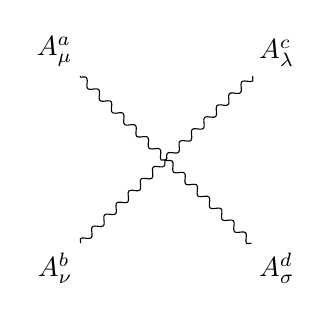
\begin{tikzpicture}[baseline=(current bounding box.center)]
        \begin{feynman}
            \vertex (b);
            \vertex [above left=of b] (a) {\(A^{a}_{\mu}\)};
            \vertex [below left=of b] (c) {\(A^{b}_{\nu}\)};
            \vertex [above right=of b] (f1) {\(A^{c}_{\lambda}\)};
            \vertex [below right=of b] (f2) {\(A^{d}_{\sigma}\)};
            \diagram* {
                (a) -- [boson] (b), 
                (b) -- [boson] (f1),
                (b) -- [boson] (c),
                (b) -- [boson] (f2),
            };
        \end{feynman}
        \end{tikzpicture}
    \end{center}
    \caption{The three types of vertex in Yang-Mills theories.}
    \label{fig:theory:YM-vertices}
\end{figure}

\section{Spontaneous Symmetry Breaking}
Spontaneous symmetry breaking (SSB) occurs when the lowest energy solutions to a theory do not respect the symmetries of the Lagrangian that describes it. 
A straightforward example is that of a three-dimensional ferromagnetic material cooling down from above its Curie temperature.
Above this threshold there is no magnetisation and solutions obey the $\mathrm{SO}(3)$ symmetry of the Lagranian. 
Below this threshold the ferromagnet becomes magnetised and must `choose' one of a degenerate family of lowest-energy solutions. This picks out a direction of magnetisation. The $\mathrm{SO}(3)$ symmetry of the ferromagnet has now been broken to $\mathrm{SO}(2)$ (Figure \ref{fig:theory:ferromagnet_ssb}).

\begin{figure}[h!]
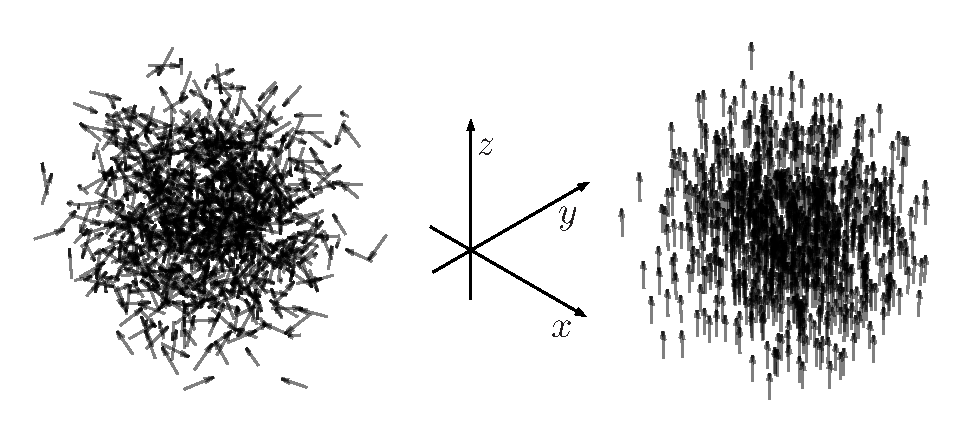
\includegraphics[width=0.8\textwidth]{figures/theory/ferromagnet_ssb.pdf}
\caption{A ferromagnet above (left) and below (right) the Curie temperature. The example below the Curie temperature has magnetised along the z-direction breaking the $\mathrm{SO}(3)$ symmetry to just $\mathrm{SO}(2)$ about the z-axis}
\label{fig:theory:ferromagnet_ssb}
\end{figure}

In the context of a field theory, symmetry can be spontaneously broken in the following way: a field experiences a potential whose minima are a family of degenerate states transforming under the symmetry group. 
Consider the Lagrangian of a complex scalar field $\phi$ experiencing a potential $V(\phi)$,
\begin{equation}
    \label{eq:theory:global_SSB_L}
    \mathcal{L} = (\partial_{\mu}\phi)^{\dag}(\partial^{\mu}\phi) - V(\phi)
\end{equation}
where the potential has the form
\begin{equation}
    \label{eq:theory:global_u1_potential}
    V(\phi) = -\mu^{2}(\phi^{\dag}\phi) + \lambda(\phi^{\dag}\phi)^{2}.
\end{equation}
This has a global $\mathrm{U}(1)$ symmetry, $\phi\rightarrow{e^{i\theta}}\phi$, and the potential has a circle of degenerate minima at $|\phi| = \frac{\mu}{\sqrt{2\lambda}} = v$. 
The vacuum expectation value (VEV) of $\phi$, $\langle\phi\rangle$ is now non-zero and will pick a state in this circle parameterised by $\langle\theta\rangle$ which can take any value $\theta_{0}$. The global symmetry has been spontaneously broken.
\begin{figure}[h!]
    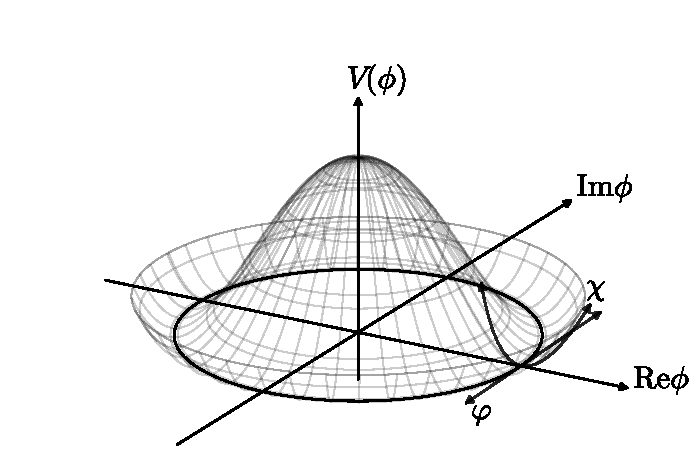
\includegraphics[width=0.5\textwidth]{figures/theory/ssb_potential.pdf}
    \caption{Perturbations around the vacuum state at $\theta_0=0$ of a symmetry breaking potential $V(\phi)$. The family of degenerate minima are shown by the black circle.}
    \label{fig:theory:global_ssb_potential}
\end{figure}
To see the effects of this SSB consider a small perturbation around the vacuum with $\theta_{0}=0$ as shown in Figure \ref{fig:theory:global_ssb_potential}. 
We describe $\phi$ in terms of two real scalar fields: one along the imaginary direction of $\phi$ (along the family of vacuum states) and one along the real (against the potential gradient),
\begin{equation}
    \phi(x) = v + \frac{1}{\sqrt{2}}(\chi(x) + i\varphi(x)).
\end{equation}
If one substitutes this into equation \ref{eq:theory:global_SSB_L} and evaluates the non-kinematic part we find that the field $\chi$ is granted a mass term of the form $\frac{1}{2}m^{2}\chi^{2}$,
\begin{equation}
    \frac{1}{2}m_{\chi}^{2}\chi^{2} = \frac{1}{2}{\lambda}v^{2}\chi^{2}
\end{equation}
and there is no equivalent term for $\varphi$. In the spectrum of this theory we now have a massive and a massless scalar boson upon quantisation. This massless boson is known as a Goldstone boson and is a general result of breaking a global symmetry: for each broken symmetry generator there is a massless Goldstone boson. 

To see this more clearly consider the case of a global $\mathrm{SU}(N)$ symmetry where the Lagrangian has the same form as before (equation \ref{eq:theory:global_u1_potential}) but $\phi$ is now a complex scalar $N$-tuplet. 
There is a global symmetry $\phi\rightarrow{e^{i\theta^{a}T^{a}}}\phi$, and a family of minima at $\phi^{\dag}\phi = \frac{\mu^{2}}{2\lambda}$ that form an $(N^{2}-1)$-dimensional surface instead of a circle. There are $(N^{2}-1)$-many ways to move on this surface and the one remaining direction is away from the centre. The former are the fields associated with the $(N^{2}-1)$ Goldstone bosons and the latter is the single massive scalar boson as before. 

\subsection{Gauge Symmetry Breaking}
In the case where we have a gauge symmetry that is spontaneously broken the behaviour is rather different: there are no Goldstone bosons and the gauge bosons are granted mass. 
To see this take the example of equation \ref{eq:theory:global_SSB_L} and consider a local $\SUN$ symmetry: we construct the gauge-covariant derivative
%
\begin{equation}
    \label{eq:theory:gauge_cov_deriv_u1}
    D_{\mu} = \partial_{\mu} + igA^{a}_{\mu}T^{a},
\end{equation}
%
replace the partial derivative, and introduce a gauge field kinetic term to get the gauge-invariant Lagrangian
\begin{equation}
    \label{eq:theory:gauge_u1_lagrangian}
    \mathcal{L} = (D_{\mu}\phi)^{\dag}(D^{\mu}\phi) - V(\phi) - \frac{1}{2}\mathrm{Tr}F_{\mu\nu}F^{\mu\nu}.
\end{equation}
%
We can consider the field $\phi$ in its ground state in terms of its norm and a local $\SUN$ transformation, and then expand around $v$,
\begin{equation}
    \label{eq:theory:phi_decomposition}
    \phi(x) = e^{i\theta^{a}(x)T^{a}}\begin{pmatrix}
        0\\
        \vdots\\
        v + \frac{1}{\sqrt{2}}H(x)
    \end{pmatrix}
\end{equation}
where $H$ is a real scalar field corresponding to the direction orthogonal to the family of vacua and  the $\theta^{a}$ correspond to the directions along its surface. The fields $\theta^{a}(x)$ now completely parameterise the vacua in contrast to the global case where it was an infinitesimal perturbation around a vacuum state.
As a result of this we recognise that the $\SUN$ transformations can always be removed by some gauge transformation $\exp(-i\theta^{a}(x)T^{a})$, so we can freely set it to zero. 
We have removed $2N-1$ degrees of freedom and we only have only one real scalar left: the gauge freedom has eliminated the Goldstone bosons from the spectrum of the theory.


When we substitute equation \ref{eq:theory:phi_decomposition} with $\theta^{a}(x)=0$ into the Lagrangian \ref{eq:theory:gauge_u1_lagrangian} and then collect the terms that contain $A_{\mu}$ we get the following Lagrangian for the gauge fields (neglecting interaction terms)
\begin{equation}
    \label{eq:theory:abelian_gaugefield_L}
    \mathcal{L}_{A} = -\frac{1}{2}\mathrm{Tr}F_{\mu\nu}F^{\mu\nu} + g^{2}v^{2}A^{a}_{\mu}A^{a\mu}
\end{equation}
This contains mass terms of the form $\frac{1}{2}m_{A}^{2}A_{\mu}A^{\mu}$, so we conclude that the fields $\theta^{a}(x)$ have indeed been eliminated and that these degrees of freedom have been absorbed into the longitudinal components of the gauge fields $A^{a}_{\mu}$ which have been granted mass $m_{A}^{2}=2g^{2}v^{2}$. 


Collecting the scalar field $H$ terms in the same way we have 
\begin{equation}
    \label{eq:theory:abelian_scalar_SSB_L}
    \mathcal{L}_{H} = \frac{1}{2}(\partial_{\mu}H)(\partial^{\mu}H) - \lambda^{2}v^{2}H^{2}% - \frac{1}{sqrt{2}} 
\end{equation}
and we conclude that the theory contains a massive scalar field with $m_{H}^{2} = 2v^{2}\lambda^{2}$ as in the global case. Upon quantisation fields such as $H$ are called Higgs bosons, and these fields have far-reaching consequences for theories of fundamental physics playing a crucial role in the SM by granting mass to all the fundamental field quanta such as electrons and quarks and by breaking part of the gauge symmetry group of the SM. 


\section{The Standard Model of Particle Physics}
The SM is a phenomenologically-motivated theory of fundamental particle interactions consisting of two Yang-Mills theories: one of the unified weak and electromagnetic interaction (electroweak theory) and one of the strong interaction (quantum chromodynamics). This section will treat these in turn using the theoretical machinery presented in previous sections. At the end of this section the resulting Higgs boson and its behaviour will then be discussed. 
\subsection{Electroweak Theory}
The electroweak unification model of Glashow, Weinberg and Salam was the birth of the SM, and our modern understanding of fundamental physics. In this subsection we will begin by constructing the interaction itself as a massless gauge theory and then break its gauge symmetry via the Brout-Englert-Higgs mechanism. We will then move on to introduce the leptonic sector and then the quark sector discussing their dynamical mass generation and properties. 

\subsubsection{Gauge Fields and the Higgs Field}
We begin with a Yang-Mills theory consisting of a complex scalar $\mathrm{SU}(2)$ doublet $\phi$ 
\begin{equation}
    \label{eq:theory:higgs_doublet}
    \phi = \begin{pmatrix}
        \phi^{+} \\
        \phi^{0}
    \end{pmatrix}
\end{equation}
and a global symmetry group $\mathcal{G}=\mathrm{SU}(2)\times\mathrm{U}(1)$ experiencing a potential $V(\phi)$ of the same form as equation \ref{eq:theory:global_u1_potential}. We build the gauge-covariant derivative 
\begin{equation}
    \label{eq:theory:electroweak_cov_deriv}
    D_{\mu} = \partial_{\mu}\mathbb{1} + {ig}W_{\mu}^{a}T^{a} + \frac{ig'}{2}yB_{\mu}\mathbb{1}
\end{equation}
where $W_{\mu}^{a}$ are the gauge fields corresponding to each of the generators of the $\mathrm{SU}(2)$ subgroup of $\mathcal{G}$, the $\tau^{a}$ are the $\mathrm{SU}(2)$ generators (Pauli Matrices), $B_{\mu}$ is the gauge field corresponding to the Abelian subgroup $\mathrm{U}(1)$, and $g$,$g'$ are the gauge couplings corresponding to the $\mathrm{SU}(2)$ and $\mathrm{U}(1)$ respectively. 
The internal field space here has two complex dimensions and the internal geometry corresponds to unit circle in the 2D complex space ($\mathrm{SU}(2)$) warped by a position-dependent complex phase ($\mathrm{U}(1)$).


We construct the following Lagrangian for the complex scalar theory
\begin{equation}
    \label{eq:theory:electroweak_scalar_lagrangian}
    \mathcal{L} = (D_{\mu}\phi)^{\dag}(D_{\mu}\phi) - V(\phi) - \frac{1}{2}\mathrm{Tr}F_{\mu\nu}F^{\mu\nu} - \frac{1}{4}G_{\mu\nu}G^{\mu\nu}
\end{equation}
where $G_{\mu\nu} = \partial_{\mu}B_{\nu} - \partial_{\nu}B_{\mu}$ is the Abelian field strength tensor.
When $\mu^{2} > 0$, $\phi$ adopts a ground state from the family of minima, gains a non-zero vacuum expectation value (VEV) and breaks the $\mathrm{SU}(2)$ subgroup. 
As described previously the $\mathrm{SU}(2)$-associated weak gauge fields will gain mass terms, but there are extra complications. Consider the gauge fields in terms of their physical states $W_{\mu}^{\pm}$
\begin{equation}
    \label{eq:theory:physical_W_states}
    W^{\pm}_{\mu} = \frac{1}{\sqrt{2}}(W^{1}_{\mu}{\mp}iW^{2}_{\mu})
\end{equation}
and the isospin structure of $D_{\mu}$ is shown explicity by writing it in matrix form

\begin{equation}
    \label{eq:theory:explicit_covderiv_ew}
    D_{\mu} = 
    \begin{pmatrix}
        \partial_{\mu} & 0 \\
        0 & \partial_{\mu} \\
    \end{pmatrix} + 
    \frac{ig}{\sqrt{2}}
    \begin{pmatrix}
        0 & W_{\mu}^{+} \\
        W_{\mu}^{-} & 0  \\
    \end{pmatrix} +
    \frac{i}{2}
    \begin{pmatrix}
        gW_{\mu}^{3} + g'yB_{\mu} & 0 \\
        0 & -gW_{\mu}^{3} + g'yB_{\mu} \\
    \end{pmatrix}.
\end{equation}
Note that both the third component of the $\mathrm{SU}(2)$ gauge field and $B_{\mu}$ both multiply a diagonal matrix in the internal isospin space, as a result of this the symmetry breaking pattern is more complex and the two fields will later need to be unmixed. 
If we substitute this expression into the Lagrangian (equation \ref{eq:theory:electroweak_scalar_lagrangian}) and gather terms quadratic in the fields we have,
\begin{equation}
    \label{eq:theory:electroweak_scalar_quad}
    \begin{split}
    \mathcal{L} =& (\partial_{\mu}H)(\partial^{\mu}H) - 4\lambda{v}^{2}H^{2} \\
                 &+ \frac{1}{2}g^{2}v^{2}W_{\mu}^{+}W^{\mu -} \\
                 &+ \frac{1}{4}v^{2}(gW_{\mu}^{3} - g'yB_{\mu})(gW^{\mu 3} - g'yB^{\mu}) \\
                 &- \frac{1}{2}\mathrm{Tr}F_{\mu\nu}F^{\mu\nu} - \frac{1}{4}G_{\mu\nu}G^{\mu\nu} \\
    \end{split}.
\end{equation}
We observe that there is a mass term present for the Higgs field $H$ and the charged weak bosons $W^{\pm}$, however, the quadratic terms for $W^{3}$ and $B$ are `mixed' and we do not have a simple mass term for $W^{3}$ and a massless $B$ field. These fields must be unmixed by performing a rotation in the internal field space 
\begin{equation}
    \begin{split}
    A_{\mu} =& \cos{\theta_{W}}B_{\mu} + \sin{\theta_{W}}W_{\mu}^{3} \\
    Z_{\mu} =& -\sin{\theta_{W}}B_{\mu} + \cos{\theta_{W}}W_{\mu}^{3} \\
    \end{split}
    \label{eq:theory:mass_diag_fields}
\end{equation}
where $\theta_{W}$ is called the weak mixing angle and is defined as $\tan{\theta_{W}} = g'/g$. The field $Z_{\mu}$ now picks up a mass term,
\begin{equation}
    \frac{1}{2} m_{Z}^{2} Z_{\mu} Z^{\mu} = \frac{1}{4}v^{2}(g^{2}+g'{^2})^{2}Z_{\mu}Z^{\mu}
    \label{eq:theory:Z_mass}
\end{equation}
and the field $A_{\mu}$ does not have a mass term. Upon quantisation these are the neutral weak boson, Z, and the photon of electromagnetism.
We can also examine the Abelian part of the gauge covariant derivative with the unmixed fields, 
\begin{equation}
    D_{\mu}^{\mathrm{Abel}} = \partial_{\mu} + ig\sin{\theta_{W}}(T^{3} + \frac{1}{2}y)A_{\mu}
    \label{eq:theory:charge_operator}
\end{equation}
this leads to the interpretation of $T^{3} + \frac{1}{2}y$ as the electromagnetic charge operator where $T^{3}$ is the third component of weak isospin and $y$ is the hypercharge.


We now have four vector bosons and one scalar boson: the three weak bosons of the weak interaction $(W_{\mu}^{\pm},Z_{\mu}^{0})$, the photon $(A_{\mu})$ of the electromagnetic interaction and the Higgs boson $(H)$ with the quantum numbers shown in table \ref{tab:theory:elecroweak_qn_bosons}.
\begin{table}[h!]
\begin{tabular}{ l | c | c | c }
    Particle & Weak isospin third component ($t_{3}$) & Weak hypercharge ($y$) & $Q = t_3 + \frac{y}{2}$ \\
    \hline
    $W^{\pm}$  & $\pm{1}$ & 0 & $\pm1$ \\
    $Z^{0}$    & 0 & 0 & 0 \\
    $\gamma$    & 0 & 0 & 0 \\
    $H$        & $-\frac{1}{2}$ & 1 & 0 \\
\end{tabular}
\caption{Electroweak quantum numbers of the electroweak gauge bosons and the Higgs boson}
 \label{tab:theory:elecroweak_qn_bosons}
\end{table}

\subsubsection{Leptons}
Leptons, fermionic constituents of the SM that interact only via electroweak interactions, must be introduced in a more careful fashion than in equation \ref{eq:theory:int_dirac_gauge_dynamics}. 
Firstly, neutrinos are assumed massless in the SM (but this not the case in nature).
Experiment also demonstrates that neutrinos only interact with left-handed chirality, and that there are processes involving the decay of $W^{-}\rightarrow{}e^{-}+\bar{\nu_{e}}$. Therefore we begin by assigning each lepton and their counterpart neutrino to a weak isodoublet with $T_{3} = \pm\frac{1}{2}$ 
\begin{equation}
    \label{eq:theory:lepton_isodoublets}
    \begin{pmatrix}
        \nu_{e} \\
        e^{-} \\
    \end{pmatrix},
    \begin{pmatrix}
        \nu_{\mu} \\
        \mu^{-} \\
    \end{pmatrix},
    \begin{pmatrix}
        \nu_{\tau} \\
        \tau^{-} \\
    \end{pmatrix}.
\end{equation}
However, the fact that there are no right-handed neutrino interactions necessitates a different structure: we need to split the leptonic isodoublets into left and right-handed versions with the projection operator
\begin{equation}
    \ell_{e} =\begin{pmatrix}
        \nu_{e} \\
        e_{L}^{-}
    \end{pmatrix},
    e^{-}_{L} = \frac{1-\gamma^{5}}{2}e^{-}
\end{equation}
and we note that the $\mathrm{SU}(2)$ gauge symmetry is actually $\mathrm{SU}(2)_{L}$ which denotes operation with the chirality operator along with the elements of the group, and the $L$ subscript has been omitted from the neutrino field as it is assumed that they are only left-handed. 
We can also write the right-handed leptons doublets as
\begin{equation}
    \label{eq:theory:right_handed_leptons}
    \begin{pmatrix}
        \frac{1-\gamma^{5}}{2}\nu_{e} \\
        \frac{1-\gamma^{5}}{2}e^{-}
    \end{pmatrix}=\begin{pmatrix}
        0 \\
        e_{R}^{-}
    \end{pmatrix},
\end{equation}
this transforms as a singlet under $\mathrm{SU}(2)_{L}$ due to the properties of the projection operator. The electroweak quantum numbers of the leptonic families are shown in table \ref{tab:theory:elecroweak_qn_leptons}
\begin{table}[h!]
\begin{tabular}{ l | c | c | c }
    Particle & Weak isospin third component ($t_{3}$) & Weak hypercharge ($y$) & $Q = t_3 + \frac{y}{2}$ \\
    \hline
    $\nu_{e},\nu_{\mu},\nu_{\tau}$  & $\frac{1}{2} $ & $-1$ & $0$ \\
    $\bar{e}_{L},\bar{\mu}_{L},\bar{\tau}_{L}$  & $-\frac{1}{2} $ & $-1$ & $-1$ \\
    $\bar{e}_{R},\bar{\mu}_{R},\bar{\tau}_{R}$  & $0$  & $-2$ & $-1$ \\
\end{tabular}
\caption{Electroweak quantum numbers of the leptons}
 \label{tab:theory:elecroweak_qn_leptons}
\end{table}

To preserve gauge invariance (due to the singlet nature of the right-handed leptons), and to grant mass only to the lower component of the lepton weak isodoublets, mass is granted dynamically via Yukawa couplings. For each isodoublet there is a coupling to the Higgs field $\phi$ of the form
\begin{equation}
    \label{eq:theory:lepton_yukawa}
    g_{f}(\bar{e}_{R}\phi^{\dag}\ell_{e} + \bar{\ell}_{e}\phi{e}_{R}),
\end{equation}
which is invariant under $\mathrm{SU}(2)_{L}$. Upon spontaneous symmetry breaking the Higgs vacuum expectation value generates mass terms and interactions with the Higgs field of the form
\begin{equation}
    \label{eq:theory:lepton_mass_higgs_int}
    g_{f}v(\bar{e}_{R}e_{L} + \bar{e}_{L}e_{R}) + g_{f}(\bar{e}_{R}e_{L}H + \bar{e}_{L}e_{R}H)
\end{equation}
where we recognise the left hand part of the expression as a fermionic mass term with $m_{f} = g_{f}v$, where $g_f$ is the Yukawa coupling strength. The Lagrangian of the leptonic sector of the SM is then
\begin{equation}
    \begin{split}
    \mathcal{L} =& -\frac{1}{2}\mathrm{Tr}F_{\mu\nu}F^{\mu\nu} - \frac{1}{4}G_{\mu\nu}G^{\mu\nu} \\
                 &+ (D_{\mu}\phi)^{\dag}(D_{\mu}\phi) + \mu^{2}(\phi^{\dag}\phi) - \lambda(\phi^{\dag}\phi)^{2} \\
                 &+ i\sum_{f=e,\nu,\tau}(\bar{\ell}_{f}\gamma^{\mu}D_{\mu}\ell_{f} + g_{f}(\bar{f}_{R}\phi^{\dag}\ell_{f} + \bar{\ell}_{f}\phi{f}_{R})) \\
                 &+ i\sum_{f=e,\nu,\tau}(\bar{f}_{R}\gamma^{\mu}D^{Y}_{\mu}f_{R}), \\
    \end{split}
\end{equation}
where $D^{Y}_{\mu}$ denotes the part of the covariant derivative that corresponds to the hypercharge, and $f$ labels lepton generation. 

\subsubsection{Quarks}
To complete the fermionic content of the SM we must include quarks: fermions with fractional electric charge that transform non-trivially under the full SM gauge group. 
In analogy with the leptons we begin by grouping the quarks into three generations of $\mathrm{SU}(2)_{L}$ isodoublets with $T_{3} = \pm\frac{1}{2}$
\begin{equation}
    \label{eq:theory:quark_isodoublets}
    \begin{pmatrix}
        u \\
        d \\
    \end{pmatrix},
    \begin{pmatrix}
        c \\
        s \\
    \end{pmatrix},
    \begin{pmatrix}
        t \\
        b \\
    \end{pmatrix},
\end{equation}
where from left to right and top to bottom we have the up, down, charm, strange, top and bottom quarks. There are also right-handed singlet fields for each flavour of quark. 

The introduction of the electroweak interaction is performed in the same way as before with the introduction of the covariant derivative and the breaking of the $\mathrm{SU}(2)_{L}$ subgroup by the Higgs mechanism. The quantum numbers of the quarks are shown in table \ref{tab:theory:elecroweak_qn_quarks}.
\begin{table}[h!]
\begin{tabular}{ l | c | c | c }
    Particle & Weak isospin third component ($t_{3}$) & Weak hypercharge ($y$) & $Q = t_3 + \frac{y}{2}$ \\
    \hline
    $u,c,t$ & $\frac{1}{2}$ & $\frac{1}{3}$ & $\frac{2}{3}$\\ 
    $d,s,b$ & $-\frac{1}{2}$ & $\frac{1}{3}$ & $-\frac{1}{3}$\\ 
    $u_{R},c_{R},t_{R}$    & $0$ & $\frac{4}{3}$ & $\frac{2}{3}$\\ 
    $d_{R},s_{R},b_{R}$    & $0$ & $-\frac{2}{3}$ & $-\frac{1}{3}$\\ 
\end{tabular}
\caption{Electroweak quantum numbers of the quarks}
\label{tab:theory:elecroweak_qn_quarks}
\end{table}

However, the mechanism for the generating quark masses is slightly different. One still uses couplings of the same form as before, but a few modifications are required to generate masses for the up-type quarks which would remain massless if we proceeded in the exact same way as for leptons. Firstly, note that the following also transforms as an $\mathrm{SU}(2)_{L}$ doublet 
\begin{equation}
    \phi_{C} = i\tau_{2}\phi^{*} = 
    \begin{pmatrix}
        \phi^{0*} \\
        -\phi^{+*}\\
    \end{pmatrix},
    \langle{\phi_{C}}\rangle = 
    \begin{pmatrix} 
        v \\ 
        0 \\ 
    \end{pmatrix},
\end{equation}
where $\tau_{2}$ is the second Pauli matrix. Now, when the Higgs isodoublet gains a vacuum expectation value this transformed version has the value in the upper part of the isodoublet and one can use this to construct gauge-invariant masses for the quarks of the following form
\begin{equation}
    \sum_{i=1,2,3}g_{i}(
    \bar{u}_{iR}\phi^{\dag}q_{iL} 
    + \bar{d}_{iR}\phi^{\dag}_{C}q_{iL}
    + \mathrm{h.c.})
\end{equation}
where h.c. denotes Hermitian conjugate. This grants equal masses to the up and down-type quarks in disagreement with experiment. We therefore have to introduce matrix-valued couplings which mix the flavours
\begin{equation}
    \sum_{i,j=1,2,3}g(
      \alpha_{ij}\bar{u}_{iR}\phi^{\dag}q_{jL} 
      + \beta_{ij}\bar{d}_{iR}\phi^{\dag}_{C}q_{jL}
      + \mathrm{h.c.}).
\end{equation}
Finally, in the physical flavour-changing currents of the SM it is combinations of down type quarks that appear. Each type of quark is measured to have a preference for their own generation but can also decay through the weak interaction to others. We can consider the down-type quarks to be `rotated' in flavour space such that the lower component of the quark isodoublets are actually mixed between $d,s,b$. We therefore replace the down part of each with 
\begin{equation}
    \begin{pmatrix}
        u \\
        d{'} \\
    \end{pmatrix},
    \begin{pmatrix}
        c \\
        s{'} \\
    \end{pmatrix},
    \begin{pmatrix}
        t \\
        b{'} \\
    \end{pmatrix},
    q{'}_{f} = \sum_{f'=d,s,b}V_{ff'}q_{f'}
\end{equation}
where the $V_{ff'}$ are elements of the Cabbibo-Kobayashi-Maskawa (CKM) matrix, a unitary matrix that performs the required rotation in flavour space.

\subsection{Quantum Chromodynamics}
As mentioned previously quarks are the only fermions of the SM to transform non-trivially under the full SM gauge group. This means that they experience an extra interaction from the gauging of the $\mathrm{SU}(3)$ subgroup, the strong interaction, and carry colour charge. This is described by quantum chromodynamics (QCD), the other Yang-Mills theory which constitutes the SM. 

To construct the Lagrangian of QCD we begin by defining the $\mathrm{SU}(3)$ covariant derivative
\begin{equation}
    D_{\mu} = \partial_{\mu} + ig_{s}t^{a}A^{a}_{\mu}
\end{equation}
where $t^{a}$ are the generators of $\mathrm{SU}(3)$, and $g_{s}$ is QCD gauge coupling. Then replace $\partial_{\mu}$ in a Dirac-type Lagrangian that has the corresponding non-Abelian field strength tensor $F^{a}_{\mu\nu}$ and whose fermions are the six flavours of quarks. 
Each of these are isodoublets that also carry the colour charge $q^{C}_{f}$, $C=R,G,B$ (red, green, blue) and are structured in colour triplets transforming under $\mathrm{SU}(3)$
\begin{equation}
    \psi_{f} = \begin{pmatrix}
        q_{f}^{R} \\
        q_{f}^{G} \\
        q_{f}^{B} \\
    \end{pmatrix}.
\end{equation}
The Lagrangian is then
\begin{equation}
    \mathcal{L}_{\mathrm{QCD}} = \sum_{f}i\bar{\psi}_{f}\gamma^{\mu}D_{\mu}\psi_{f} - \frac{1}{2}\mathrm{Tr}F_{\mu\nu}F^{\mu\nu}
\end{equation}
where the index $f$ denotes quark flavour. Upon quantisation we will have eight massless gauge bosons called gluons that couple to quark pairs of the same flavour. 

The strong interaction behaves differently to the weak or electromagnetic interactions: instead of the weakening with distance the strong force increases in strength. An important result of this phenomenon is that colour-carrying particles such as quarks and gluons are confined and can only exist within composite particles called hadrons. This is responsible for the phenomenon of jets in high-energy particle collisions. Jets are cone-shaped sprays of particles where a quark or gluon has been produced, cannot exist freely and then hadronizes. 

We now have the full fundamental particle content of the SM and the couplings between them. Next we will consider how the above is manifested as the phenomenology of the Higgs boson.


\subsection{Higgs boson phenomenology}
The Higgs boson couples directly to every massive particle in the SM: either through the gauge-covariant derivative that gives interactions with the weak gauge bosons, or the Yukawa couplings which cause interaction with the non-neutrino fermions. In this section we will look at how Higgs bosons are created in proton-proton collisions at the Large Hadron Collider, and then how they decay.

\subsubsection{Higgs boson production in proton collisions}
There are four main ways that a Higgs boson can be produced in proton collisions: gluon fusion (ggH), vector boson fusion (VBF), associated production (VH), and top fusion (\ttH) (Figure \ref{fig:theory:higgs_production}). 
\begin{figure}[h!]
    \begin{center}
        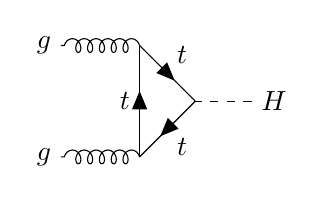
\begin{tikzpicture}[baseline=(current bounding box.center)]
        \begin{feynman}
            \vertex (a) {\(H\)};
            \vertex [left=1cm of a] (b);
            \vertex [above left=1cm of b] (c);
            \vertex [below left=1cm of b] (d);
            \vertex [left=1cm of c] (e) {\(g\)};
            \vertex [left=1cm of d] (f) {\(g\)};
            \diagram* {
                (a) -- [scalar] (b),
                (c) -- [fermion,edge label=\(t\)] (b),
                (d) -- [fermion,edge label=\(t\)] (c),
                (b) -- [fermion,edge label=\(t\)] (d),
                (c) -- [gluon] (e),
                (d) -- [gluon] (f)
            };
        \end{feynman}
        \end{tikzpicture}
         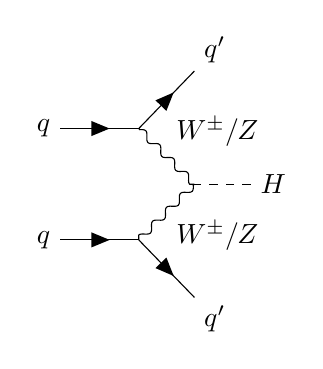
\begin{tikzpicture}[baseline=(current bounding box.center)]
             \begin{feynman}
            \vertex (a) {\(H\)};
            \vertex [left=1cm of a] (b);
            \vertex [above left=1cm of b] (c);
            \vertex [below left=1cm of b] (d);
            \vertex [left=1cm of c] (e) {\(q\)};
            \vertex [left=1cm of d] (f) {\(q\)};
            \vertex [above right=1cm of c] (g) {\(q{'}\)};
            \vertex [below right=1cm of d] (h) {\(q{'}\)};
            \diagram* {
                (a) -- [scalar] (b),
                (c) -- [boson,edge label=\(W^{\pm}/Z\)] (b),
                (b) -- [boson,edge label=\(W^{\pm}/Z\)] (d),
                (c) -- [fermion] (g),
                (d) -- [fermion] (h),
                (e) -- [fermion] (c),
                (f) -- [fermion] (d)
            };
        \end{feynman}
        \end{tikzpicture}       
%    \end{center}
%    \begin{center}
        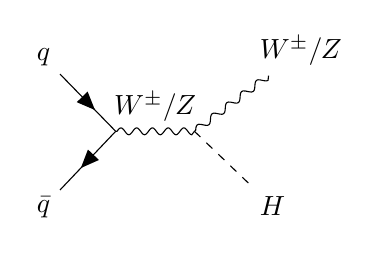
\begin{tikzpicture}[baseline=(current bounding box.center)]
        \begin{feynman}
            \vertex (b);
            \vertex [above left=1cm of b] (a) {\(q\)};
            \vertex [below left=1cm of b] (c) {\(\bar{q}\)};
            \vertex [right=1cm of b] (d);
            \vertex [below right=1cm of d] (e) {\(H\)};
            \vertex [above right=1cm of d] (f) {\(W^{\pm}/Z\)};
            \diagram* {
                (a) -- [fermion] (b),
                (b) -- [fermion] (c),
                (b) -- [boson,edge label=\(W^{\pm}/Z\)] (d),
                (d) -- [scalar] (e),
                (d) -- [boson] (f),
            };
        \end{feynman}
        \end{tikzpicture}
        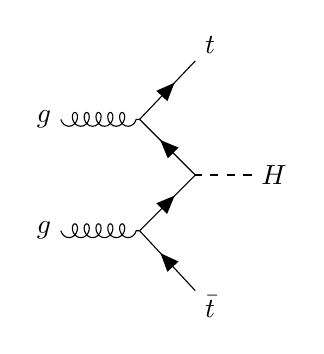
\begin{tikzpicture}[baseline=(current bounding box.center)]
        \begin{feynman}
            \vertex (a) {\(H\)};
            \vertex [left=1cm of a] (b);
            \vertex [above left=1cm of b] (c);
            \vertex [below left=1cm of b] (d);
            \vertex [left=1cm of c] (e) {\(g\)};
            \vertex [left=1cm of d] (f) {\(g\)};
            \vertex [above right=1cm of c] (g) {\(t\)};
            \vertex [below right=1cm of d] (h) {\(\bar{t}\)};
            \diagram* {
                (a) -- [scalar] (b),
                (b) -- [fermion] (c),
                (d) -- [fermion] (b),
                (c) -- [fermion] (g),
                (h) -- [fermion] (d),
                (e) -- [gluon] (c),
                (f) -- [gluon] (d)
            };

        \end{feynman}
        \end{tikzpicture}
    \end{center}
    \caption{The four main production modes of the Higgs boson at the LHC. Left to right: ggH, VBF, VH and \ttH}
    \label{fig:theory:higgs_production}
\end{figure}
Gluon fusion dominates over the other processes for a Higgs boson of mass $m_{H}=125$\,GeV and proton collisions at $\sqrt{s} = 13$\,TeV with a cross section of 49\,pb. VBF is the second largest with 3.8\,pb, VH is third with 2.3\,pb and \ttH is last with $0.5$\,pb. Although ggH has by far the largest cross-section, the other production modes contain extra objects in their final state aiding the separation of Higgs bosons from events that resemble them. In particular VBF gives rise to two highly energetic jets from the final-state quarks with a large angular separation. 

\subsubsection{Higgs boson decays}
Once produced the Higgs boson is predicted to decay very quickly to pairs of particles. At tree-level it will decay into massive particles in proportion to their masses in two different ways: in the case of particles granted mass through the Yukawa couplings (fermions) the branching ratio will be proportional to the square of the mass, in the case of particles granted mass through the gauge-covariant derivative the branching ratio will be proportional to the fourth power of the mass (weak gauge bosons). 
The Higgs boson can also decay via loop diagrams that have a reduced branching ratio. The prevalence of the main decay modes are summarised in table \ref{tab:theory:higgs_branching_ratios}.
\begin{table}[h!]
\begin{tabular}{ l | c | c | c | c | c | c | c}
    Decay Mode & $b\bar{b}$ & $W^{\pm}W^{\mp*}$ & $gg$ & $\tau\bar{\tau}$ & $c\bar{c}$ & $ZZ^{*}$ & $\gamma\gamma$ \\
    \hline
    Branching ratio & 58.2\% & 21.4\% & 8.2\% & 6.3\% & 2.8\% & 2.6\% & 0.23\% \\
\end{tabular}
\caption{Main branching ratios of the Higgs boson}
 \label{tab:theory:higgs_branching_ratios}
\end{table}

The \Hgg decay (Figure \ref{fig:theory:higgs_gammagamma}) is of particular interest in experimental searches despite its relatively small branching ratio. It has a simple, fully-reconstructed final state with no composite objects such a jets or missing momentum, that causes difficulty in a high-multiplicity hadronic environment such as at the LHC. This decay mode's clean signal lead to it being one of the two channels in which the Higgs boson was discovered in 2012.
\begin{figure}[h!]
    \begin{center}
        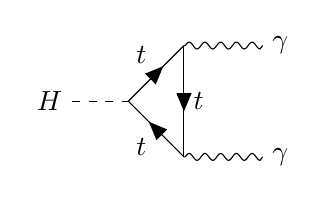
\begin{tikzpicture}[baseline=(current bounding box.center)]
        \begin{feynman}
            \vertex (a) {\(H\)};
            \vertex [right=1cm of a] (b);
            \vertex [above right=1cm of b] (c);
            \vertex [below right=1cm of b] (d);
            \vertex [right=1cm of c] (e) {\(\gamma\)};
            \vertex [right=1cm of d] (f) {\(\gamma\)};
            \diagram* {
                (a) -- [scalar] (b),
                (b) -- [fermion,edge label=\(t\)] (c),
                (c) -- [fermion,edge label=\(t\)] (d),
                (d) -- [fermion,edge label=\(t\)] (b),
                (c) -- [photon] (e),
                (d) -- [photon] (f)
            };
        \end{feynman}
        \end{tikzpicture}
        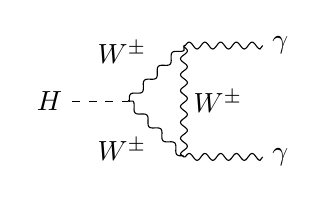
\begin{tikzpicture}[baseline=(current bounding box.center)]
        \begin{feynman}
            \vertex (a) {\(H\)};
            \vertex [right=1cm of a] (b);
            \vertex [above right=1cm of b] (c);
            \vertex [below right=1cm of b] (d);
            \vertex [right=1cm of c] (e) {\(\gamma\)};
            \vertex [right=1cm of d] (f) {\(\gamma\)};
            \diagram* {
                (a) -- [scalar] (b),
                (b) -- [photon,edge label=\(W^{\pm}\)] (c),
                (c) -- [photon,edge label=\(W^{\pm}\)] (d),
                (d) -- [photon,edge label=\(W^{\pm}\)] (b),
                (c) -- [photon] (e),
                (d) -- [photon] (f)
            };
        \end{feynman}
        \end{tikzpicture}
        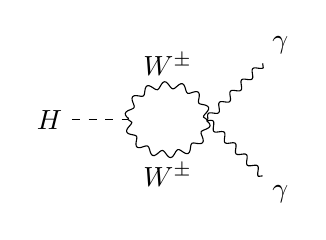
\begin{tikzpicture}[baseline=(current bounding box.center)]
        \begin{feynman}
            \vertex (a) {\(H\)};
            \vertex [right=1cm of a] (b);
            \vertex [right=1cm of b] (c);
            \vertex [above right=1cm of c] (d) {\(\gamma\)};
            \vertex [below right=1cm of c] (e) {\(\gamma\)};
            \diagram* {
                (a) -- [scalar] (b),
                (b) -- [photon, half left, edge label=\(W^{\pm}\)] (c),
                (c) -- [photon, half left, edge label=\(W^{\pm}\)] (b),
                (c) -- [photon] (d),
                (c) -- [photon] (e),
            };
        \end{feynman}
        \end{tikzpicture}
    \end{center}
    \caption{Main contributing diagrams to the Higgs diphoton decay mode.}
    \label{fig:theory:higgs_gammagamma}
\end{figure}







    \chapter{Apparatus}
\label{chap:apparatus}

%\chapterquote{This thing, what is it in itself, in its own constitution? What is its substance and material?}{Marcus Aurelius}

\newpage

\section{Introduction}
This chapter describes the experimental apparatus used to produce the 2016 proton-proton collision dataset used in this thesis. A description of the means of collision production, the Large Hadron Collider (LHC), will be given and their measurement with the Compact Muon Solenoid (CMS) will be described in particular detail. The CMS design and operation described here will correspond to the 2016 running period.

\section{The Large Hadron Collider}
The LHC \cite{LHC_design_report} is a large synchrotron-type particle accelerator whose purpose is to provide collisions to survey electroweak-scale physics, particularly the mechanism of electroweak symmetry breaking, in addition to a broad physics program which ranges from dark matter searches to flavour physics to studies of quark-gluon plasma.
These studies are afforded by the production of high-energy and high-luminosity proton and lead ion collisions in counter-circulating beams. These achieve a long reach for the production of heavy particles and superior statistical power for the study of rare processes. 
The remainder of this section will be solely concerned with the LHC's proton-proton operation.  

\subsection{LHC Accelerator Chain}

Before collisions occur at the LHC interaction points the beams must be produced and conditioned with a collection of accelerators \cite{CERN_accelerator_complex} before injection into the LHC (Figure \ref{fig:apparatus:lhc_chain}).
\begin{figure}[h!]
    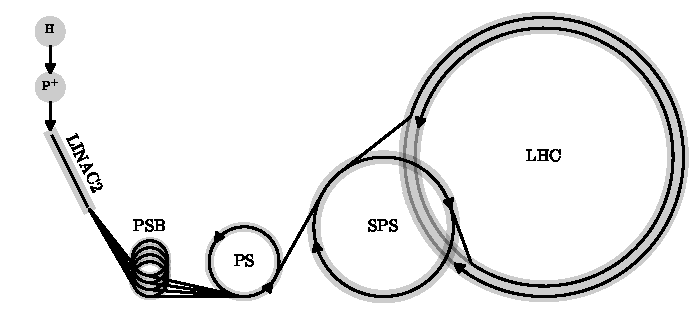
\includegraphics[width=0.9\textwidth]{figures/apparatus/accel_chain.pdf}
    \caption{A schematic view of the LHC accelerator chain for proton-proton operation.}
    \label{fig:apparatus:lhc_chain}
\end{figure}
This process begins with the acquisition of protons from a small quantity of hydrogen gas: hydrogen is injected into a chamber and the atomic electrons are stripped off using a strong electric field. The resulting bare protons are then injected into a linear accelerator (LINAC 2) and accelerated by radiofrequency (RF) cavities to an energy of 50\,MeV. The protons then enter the Proton Synchrotron Booster (PSB), which consists of four synchrotron rings stacked on top of each other with a radius of 25\,m, the protons are further accelerated up to an energy of 1.4\,GeV allowing for more protons to be injected into the next part of the accelerator chain and therefore higher-intensity beams.
The protons from each ring of the PSB enter the Proton Synchrotron (PS) in sequence with 25\,ns spacing to form the bunch structure. The PS is another synchrotron with a radius of 72\,m where they are accelerated to 25\,GeV. 
When they have reached this energy the protons are then injected into the Super Proton Synchrotron (SPS) which has a circumference of nearly 7\,km and accelerates protons to 450\,GeV before their injection into the LHC in two opposing directions. 


\subsection{LHC Structure and Operation}
The LHC itself is a 27\,km ring consisting of 1232 8\,T superconducting dipole magnets that force the protons into a circular path so they can be repeatedly accelerated by 16 superconducting RF cavities oscillating at 400\,MHz. As on-time protons with correct energy come in to the cavity they do not experience any acceleration, if they arrive slightly later they experience an accelerating potential, slightly early and they experience a deceleration. This maintains the energy of the protons and the bunch structure as they circulate in the LHC ring. The beams are then further adjusted by 392 quadrupole magnets to maintain stable beam conditions and stronger quadrupole magnets are used to focus the beams at the four LHC collision points.

Bunches of protons are brought together to collide at each of the LHC interaction points every 25\,ns during normal operation. This is referred to as a bunch crossing and usually produces multiple superimposed proton collisions (pileup) and a large dose of radiation for any equipment situated nearby. These conditions pose challenges for the design and operation of the LHC's experiments. 

The LHC is designed to operate with a centre of mass energy of $\sqrt{s}=14$\,TeV and instantaneous luminosity of $10^{34}$\,$\mathrm{cm}^{-2}\mathrm{s}^{-1}$ with two beams of 2880 bunches. During the 2016 period the LHC operated at $\sqrt{s} = 13$\,TeV and an instantaneous luminosity above design specification at $1.4\times{}10^{34}$\,$\mathrm{cm}^{-2}\mathrm{s}^{-1}$. This culminated in 40.82\,fb$^{-1}$ of integrated luminosity delivered to the CMS experiment in the 2016 period with an average pileup rate of 27 \cite{CMSLumiPublic} (Figure \ref{fig:apparatus:cms_int_lumi}).
\begin{figure}[h!]
    \begin{center}
    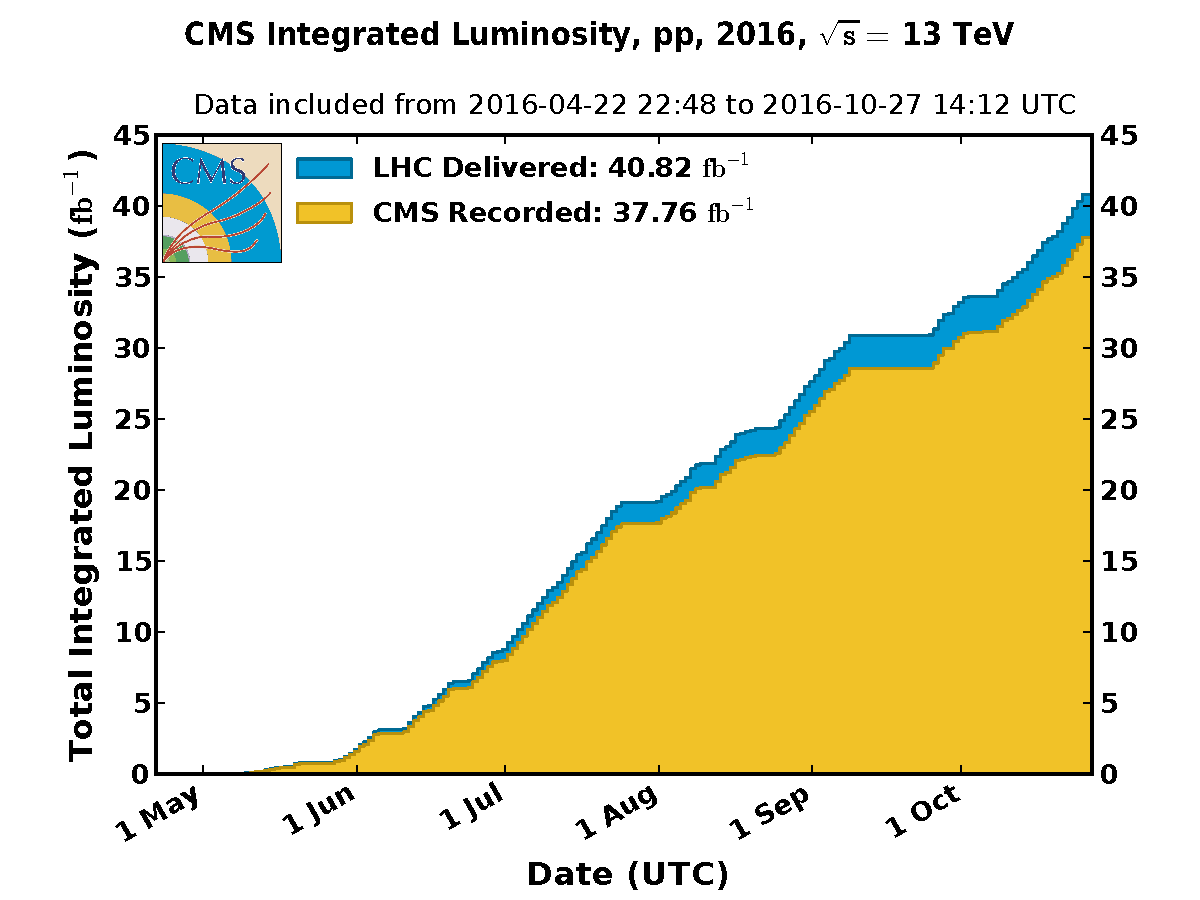
\includegraphics[width=0.49\textwidth]{figures/apparatus/int_lumi_per_day_cumulative_pp_2016.pdf}
    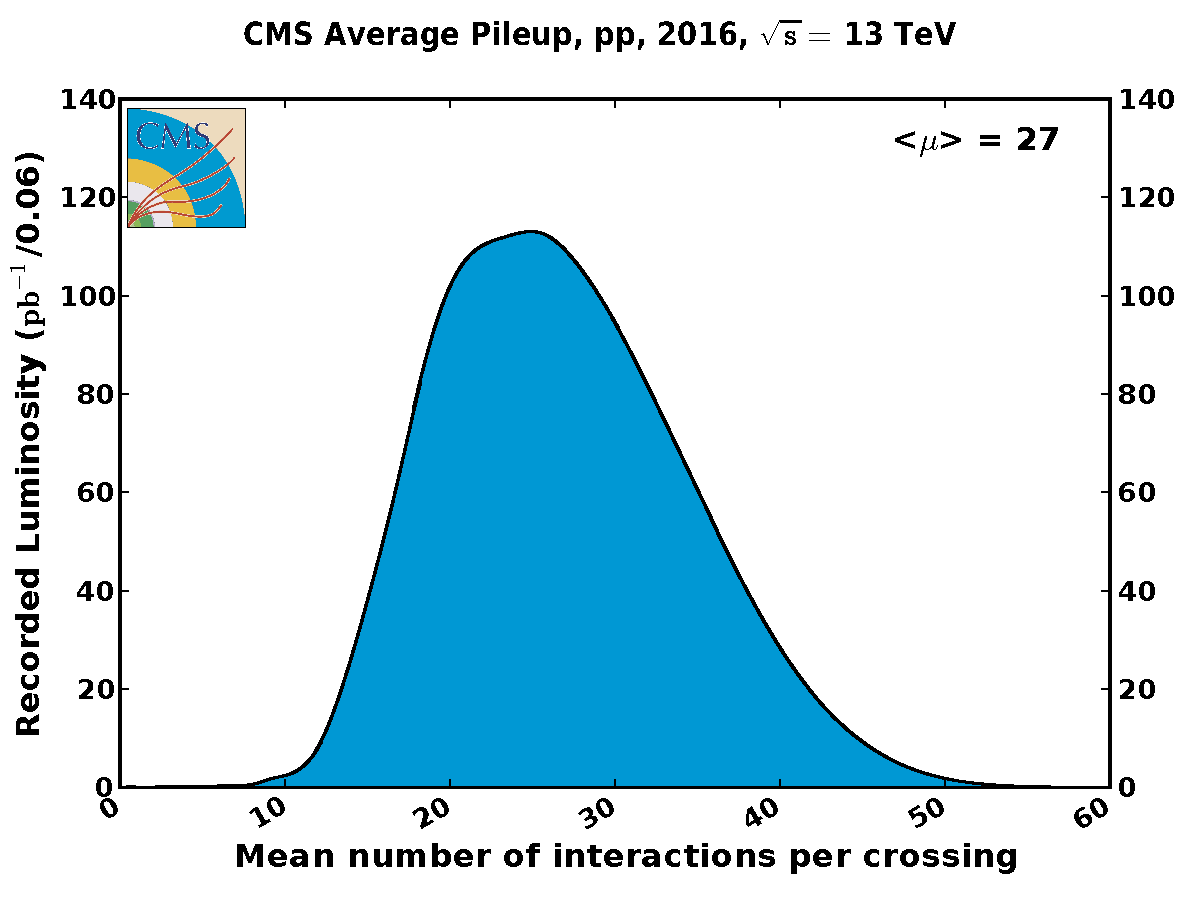
\includegraphics[width=0.49\textwidth]{figures/apparatus/pileup_pp_2016.pdf}
    \end{center}
    \caption{Left: total integrated luminosity over the 2016 proton-proton running period delivered to (blue) and recorded by (orange) the CMS experiment \cite{CMSLumiPublic}. Right: the 2016 pileup distribution \cite{CMSLumiPublic}.}
    \label{fig:apparatus:cms_int_lumi}
\end{figure}


\section{The Compact Muon Solenoid}

The CMS experiment \cite{CMSatLHC} is a general-purpose detector situated at Point 5 on the LHC directly opposite its counterpart, ATLAS \cite{AtlasatLHC}. CMS uses a right-handed coordinate system with the $x$-axis pointing horizontally towards the centre of the ring, the $y$-axis pointing vertically, and the $z$-axis pointing along the beamline in the anti-clockwise direction. 
An angular coordinate system is commonly used in physics analyses which consists of the coordinates $(\phi,\eta,z)$, where $\phi$ is the azimuthal angle in the $x$-$y$ plane and $\eta$ is the pseudorapidity defined from the polar angle $\theta$ as
\begin{equation}
    \label{eq:apparatus:pseudorapidity}
    \eta = -\ln\tan{\frac{\theta}{2}}.
\end{equation}
Generally, the high $|\eta|$ regions closer to the beamline are referred to as forward, and the low $|\eta|$ region is referred to as central. 
In addition, the radial distance in the $x$, $y$ plane $r$ is sometimes used. The different coordinates used at CMS are summarised in Figure \ref{fig:apparatus:coords}. This thesis will use the $(\phi,\eta,z)$ coordinate system. 
\begin{figure}[h!]
    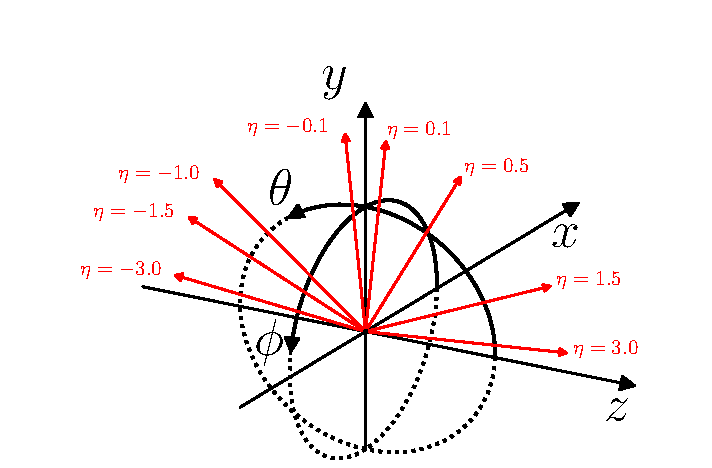
\includegraphics[width=0.45\textwidth]{figures/apparatus/CMS_coords.pdf}
    \caption{Coordinate systems used at CMS. Example values for the pseudorapidity $\eta$ are shown by the red arrows.}
    \label{fig:apparatus:coords}
\end{figure}

\subsection{Design Overview}
The design of CMS is driven by the challenges of operating in the LHC collision environment and by the broad range of its physics goals \cite{CMSPhysics}.
The LHC produces proton-proton bunch crossings at a high rate (40\,MHz) and this requires CMS to be very responsive to facilitate a short decision time on accepting an event. This high collision rate also means that the components of CMS operate in a high-radiation environment, so their performance must be robust to large doses of radiation. Finally, the pileup in each bunch crossing puts particular requirements on the CMS design to achieve isolation of different kinds of particles in a complex, high-multiplicity environment: it requires fine granularity, both spatial and temporal. 


The physics goals of CMS include the discovery and measurement of the Higgs boson and searches for supersymmetry amongst other topics like extra gauge bosons, extra dimensions and heavy ion collisions. 
The CMS Higgs physics programme has prioritised searches for the Higgs boson in the leptonic final states as well as the diphoton final state as these have superior signal separation potential and mass resolution in the LHC collision environment when compared to hadronic searches. For supersymmetry searches one expects events with a significant degree of missing-transverse energy ($E_{T}^{\mathrm{miss}}$) and this, along with maximising the acceptance of other analyses, motivates the hermetic design of CMS. Therefore, the main CMS performance goals were decided to be \cite{CMSatLHC}:
\begin{itemize}[leftmargin=.5in,noitemsep]
    \item Good identification of muons and good muon momentum resolution,
    \item Good charged particle momentum resolution and reconstruction efficiency,
    \item Efficient triggering and offline tagging for $\tau$ leptons and $b$ quark jets, 
    \item Good energy resolution for electromagnetically interacting particles over a large geometric area, and $\pi^{0}$ rejection,
    \item Good missing-transverse energy and dijet mass resolution.
\end{itemize}
The design of CMS, shown in Figure \ref{fig:apparatus:CMS}, achieves these goals. 
\begin{figure}[h!]
%    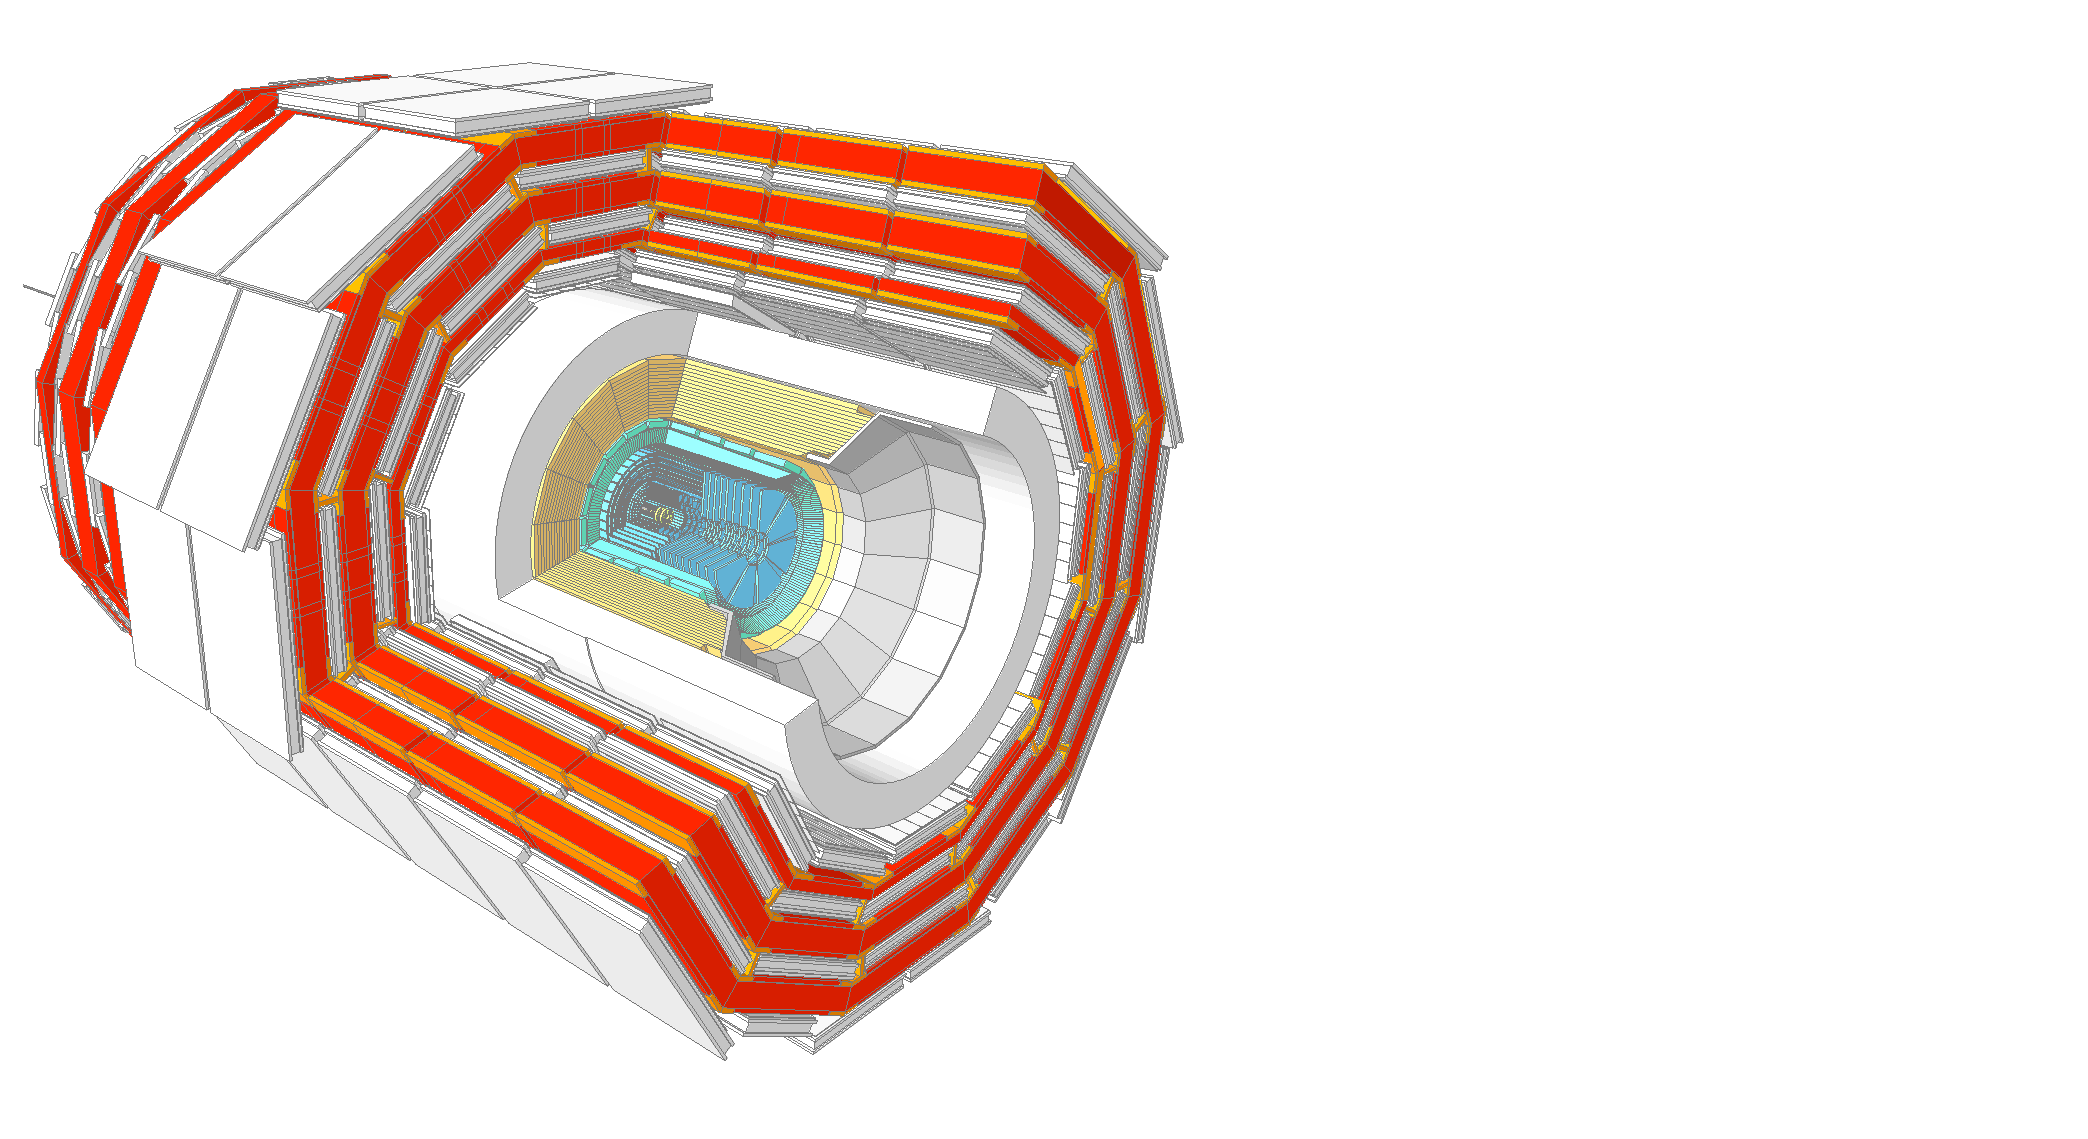
\includegraphics[width=0.9\textwidth]{figures/apparatus/CMS.pdf}
    \begin{center}
        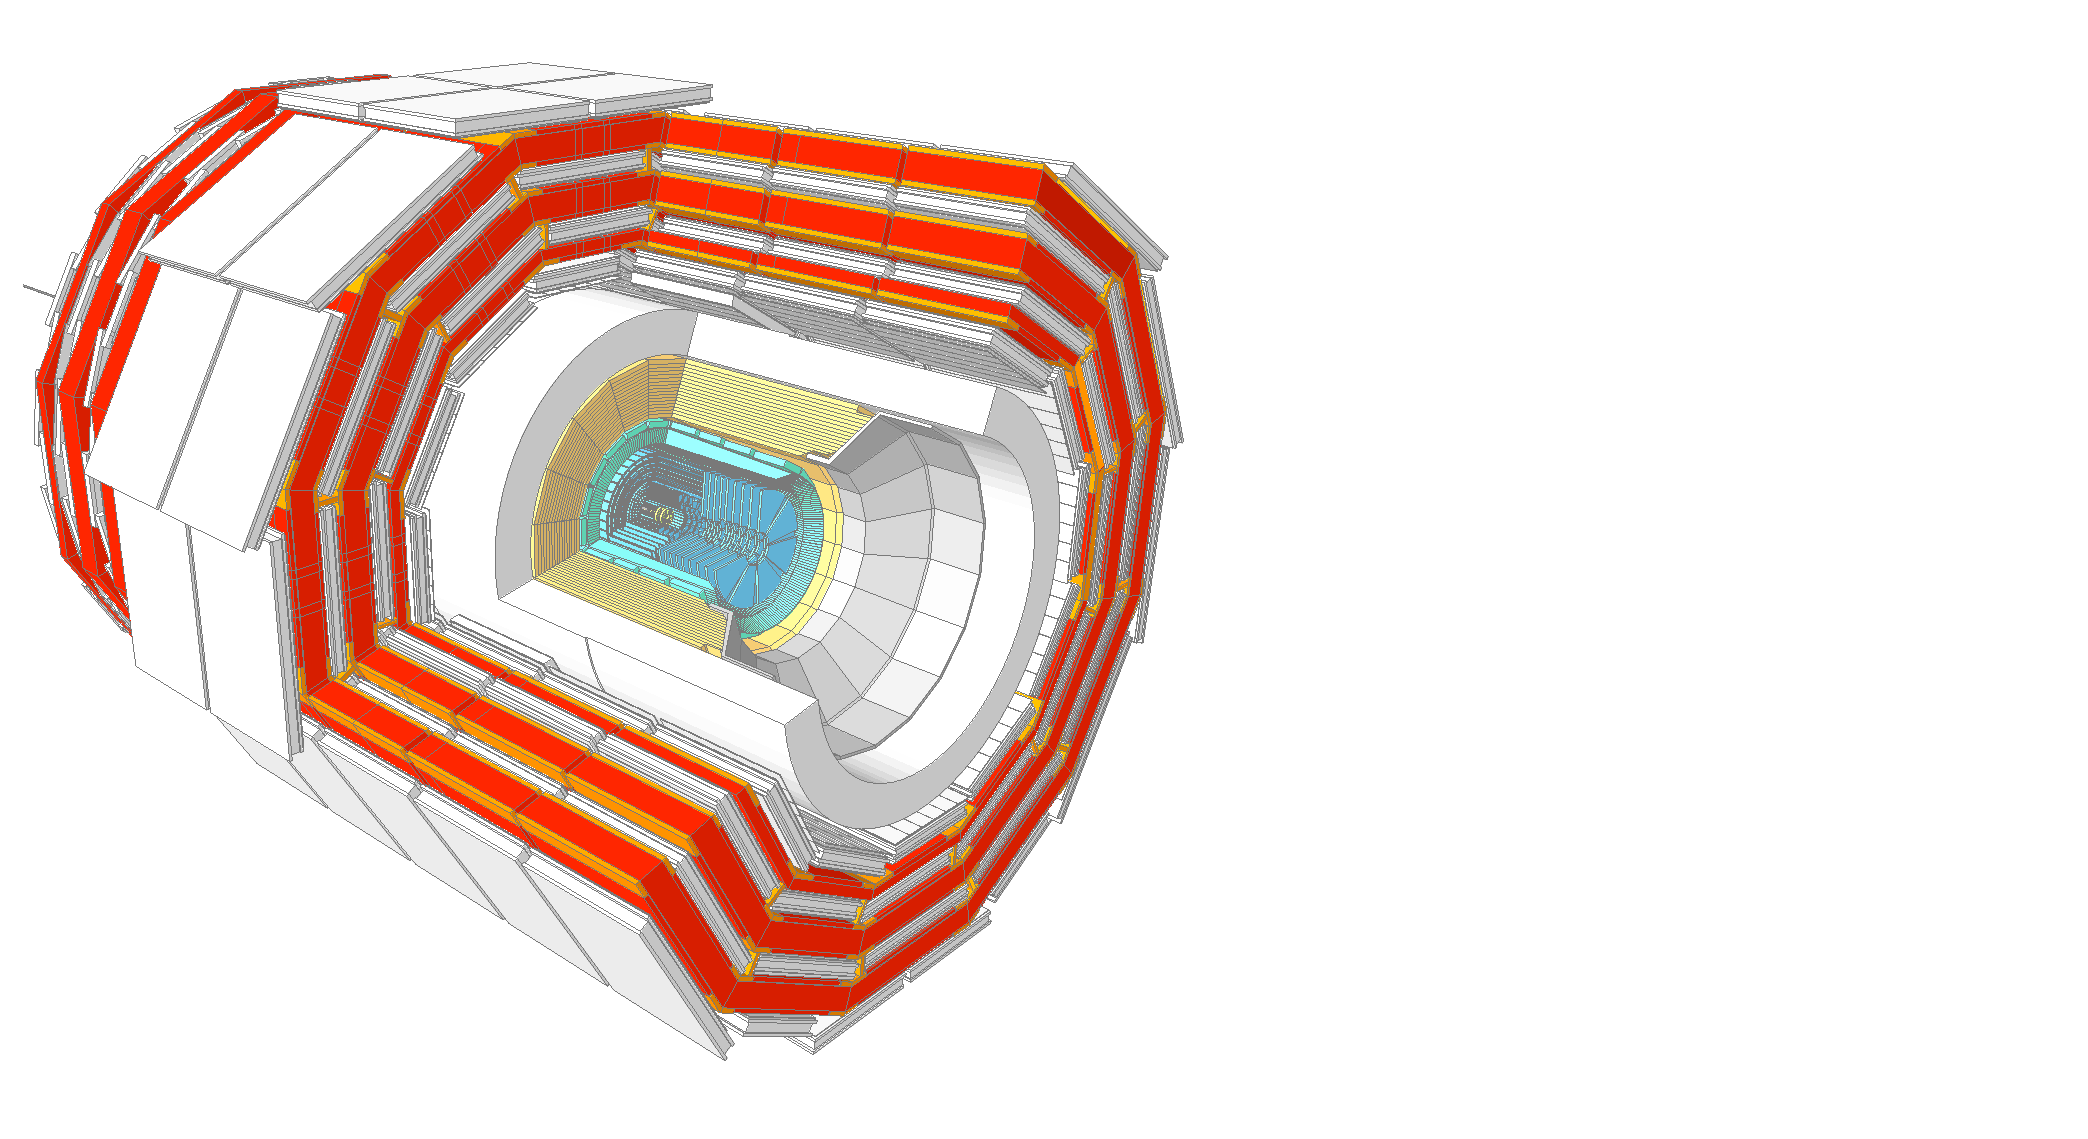
\includegraphics[width=0.57\textwidth]{figures/apparatus/CMS.pdf}
        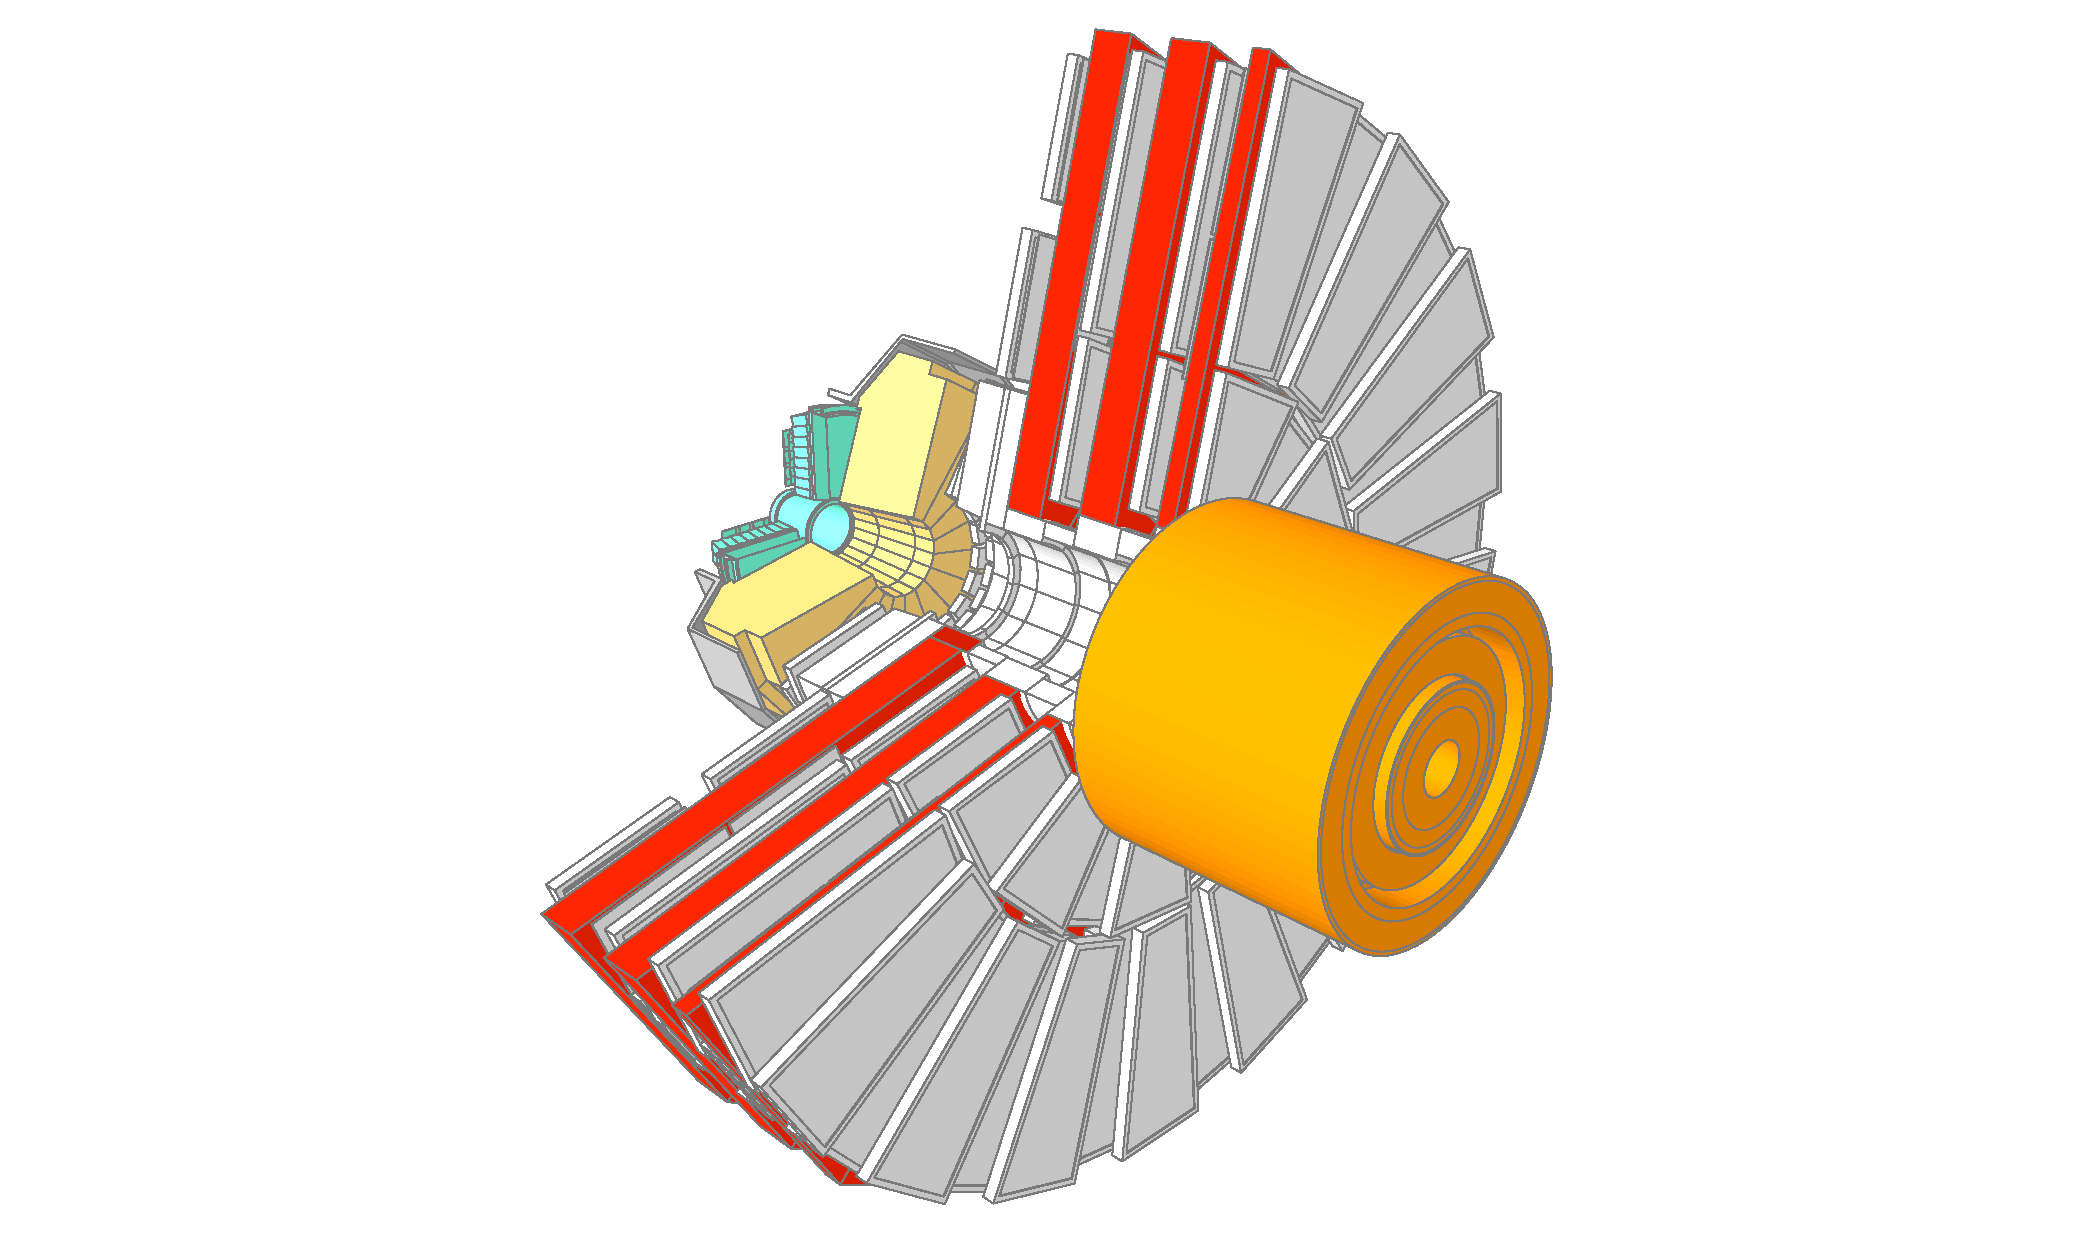
\includegraphics[width=0.42\textwidth]{figures/apparatus/ENDCAP2.pdf}
    \end{center}    
    \caption{The CMS experiment separated into barrel (left) and endcap (right), both have an azimuthal section removed to show structure of the detector subsystems. Rendering was built with the model in \cite{SketchupCMS}.}
    \label{fig:apparatus:CMS}
\end{figure}



The general structure of CMS is a classic hermetic design with a main cylindrical section centred around the interaction point called the `barrel' which is then sealed by two `endcaps' this gives a detector with a pseudorapidity range from $-5$ to $5$ that almost covers the entire $4\pi$ solid angle. Both barrel and endcaps consist of multiple concentric detector subsystems with different functionality, all of this is based around the main feature of the CMS detector: its large superconducting solenoid. 
The CMS solenoid, along with the steel return yoke it is supported by, achieves a high-strength and homogenous magnetic field over a large volume. This field bends the trajectories of charged particles into a helix, and when this bend is measured precisely one can achieve a precise momentum measurement. This meets the performance requirements for momentum resolution of charged particles and especially muons. Within the bore of the solenoid there are three subsystems: the tracker, the electromagnetic calorimeter (ECAL) and the hadron calorimeter (HCAL). The tracker consists entirely of silicon based sensors and performs precise measurements of charged particle trajectories, at the centre are pixel detectors which allow CMS to meet its $\tau$ lepton and $b$-quark jet tagging goals by reconstructing tracks and secondary vertices with great precision. 
After this, the ECAL measures the energy of electromagnetically-interacting particles with good resolution. This energy resolution allows for excellent mass resolution for dilepton and diphoton objects and is crucial to the measurement of Higgs boson decays to $\gamma\gamma$ and $ZZ^{(*)}$.
Situated around the ECAL, the HCAL measures the energies of neutral hadrons and covers a large area with fine granularity to achieve hermeticity and to meet the objective of good $E_{T}^{\mathrm{miss}}$ measurement.
Finally, the muon detectors are sited around the outside of the solenoid and cover a large area. These systems are interleaved with the steel return yoke and measure muon trajectories and energy precisely to achieve good muon momentum resolution and particle identification with a fast response. 
Each of these subdetector systems, with the exception of the tracker, provide fast measurements for the CMS trigger system. This allows CMS to cope with the very high data rate by making fast decisions about whether to keep events.
Each of these systems will be described in detail in the following subsections. Particular attention will be given to the ECAL due to its importance to the measurement of the Higgs diphoton decay mode. 


\subsection{Solenoid and Return Yoke}

The CMS magnet is a liquid helium cooled superconducting solenoid 12.5\,m in length with a bore of diameter 6\,m and a mass of 220\,t (including all systems operating at cryogenic temperature) \cite{CMSPhysics}. 
This is situated within a steel return yoke \cite{Yoke} which weighs 12000\,T extends outwards to a diameter of 14\,m and is made of five barrel `wheels' with three layers, and then completed by three disks in each endcap (Figure \ref{fig:apparatus:solenoid_yoke}).
\begin{figure}[h!]
    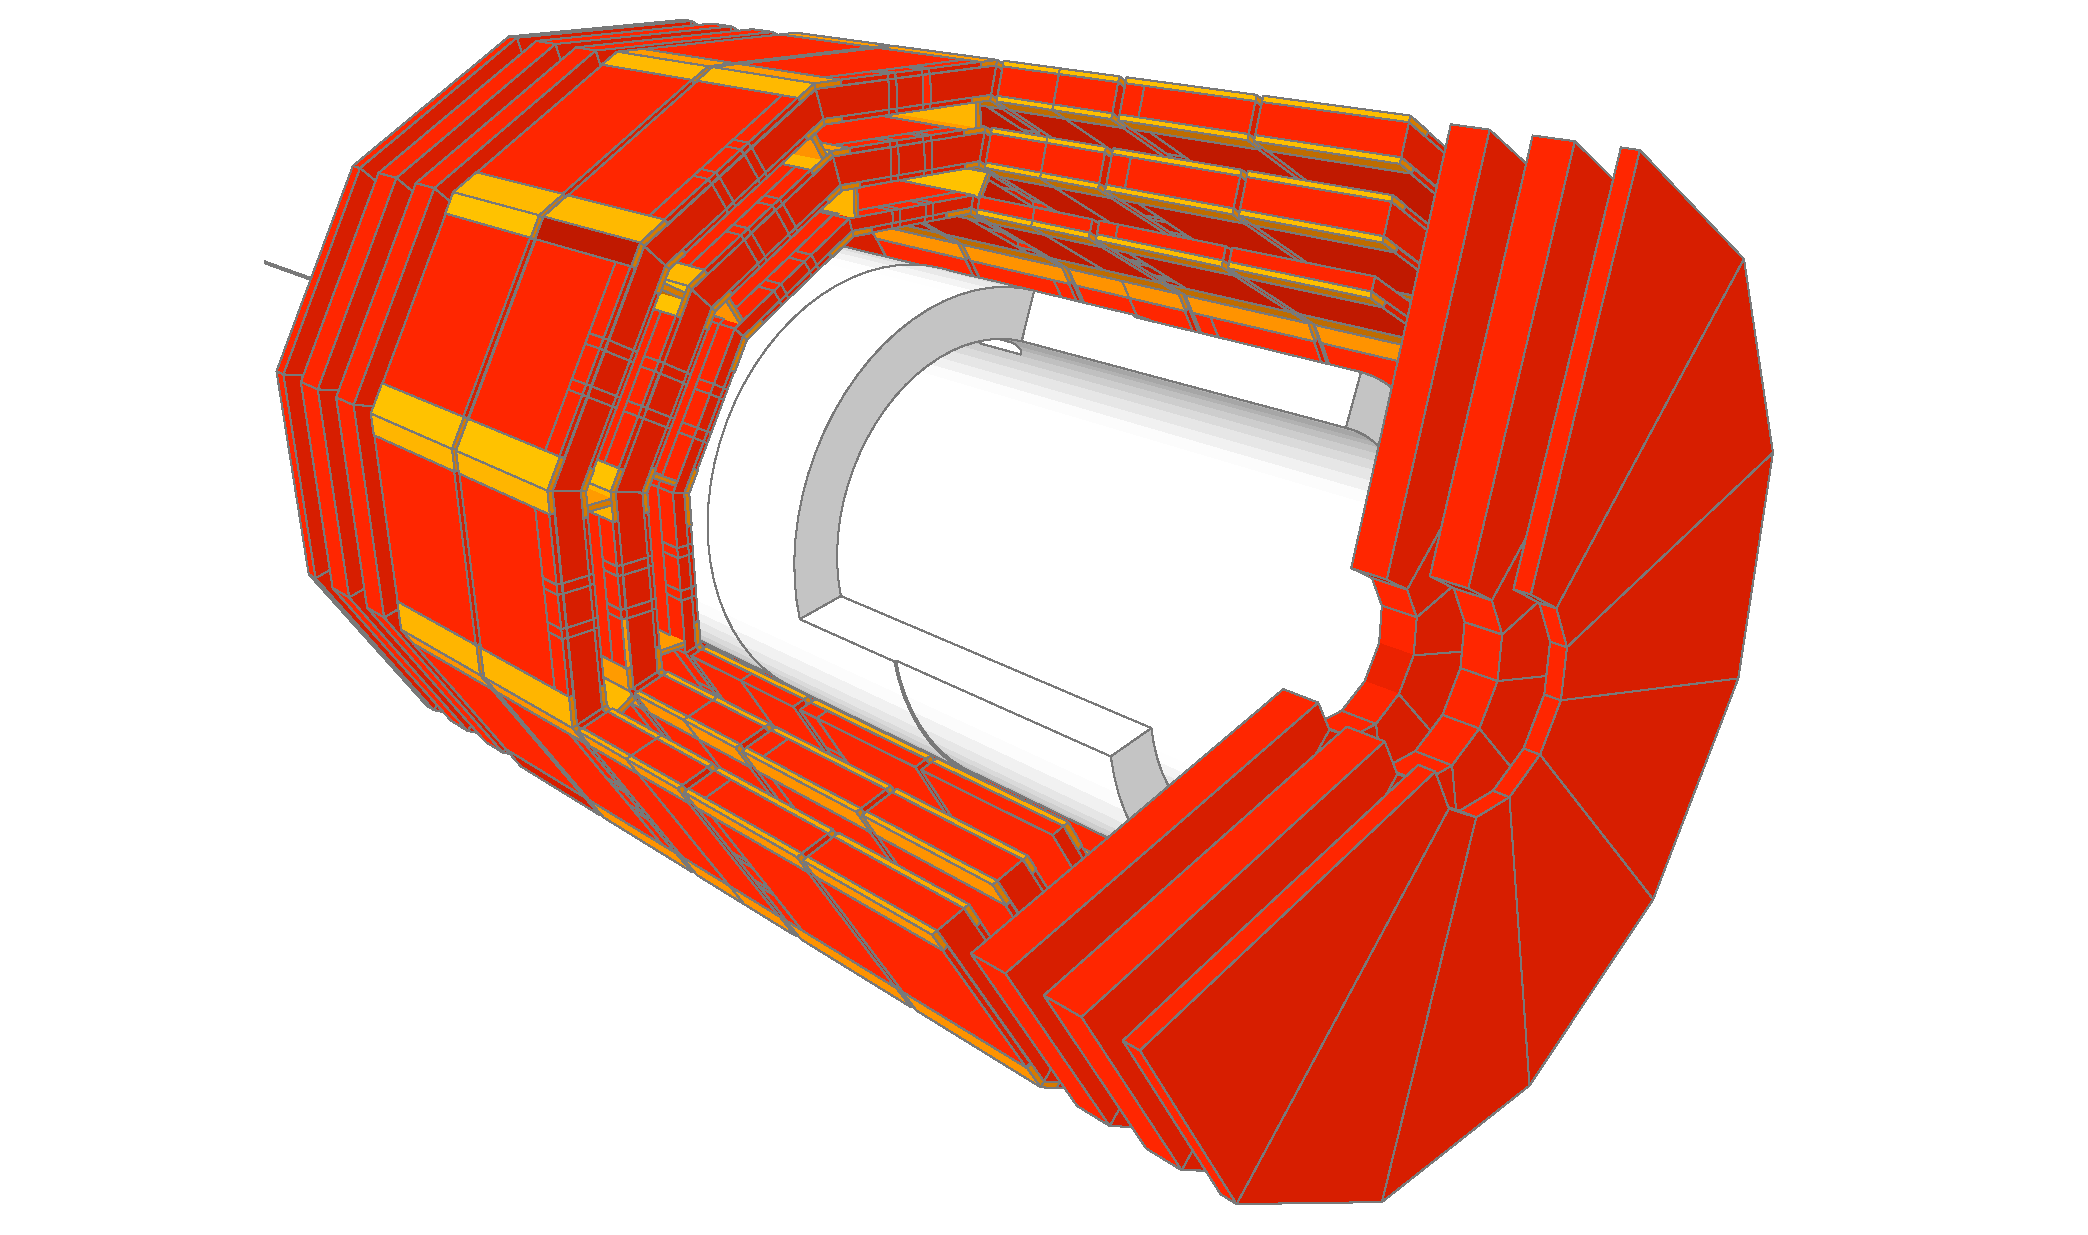
\includegraphics[width=0.5\textwidth]{figures/apparatus/solenoid_yoke.pdf}
    \caption{The CMS solenoid (white) within the steel return yoke (red). Rendering uses \cite{SketchupCMS}.}
    \label{fig:apparatus:solenoid_yoke}
\end{figure}
The niobium-titanium coils of the solenoid carry 18160\,A of current which produces a magnetic field strength within the bore of 3.8\,T and a stored energy of 2.3\,GJ. 
This field strength is below the design capability of 4\,T to maximise the operating lifetime of the solenoid.
The return yoke then conditions this field, increasing the strength in the bore by a small amount (8\%) \cite{Yoke} and improving the field homogeneity in the barrel and the muons systems. 


\subsection{Inner Tracking}

The CMS tracker \cite{CMSTrackerTDR} is the innermost detector layer and is designed to measure the trajectories and the secondary vertices of charged particles with high precision. 
To meet the requirements of the LHC operating environment the tracker must have fine granularity to handle the high-multiplicity environment, precise timing to match the particle tracks to the correct bunch crossing, and it must be robust to large doses of radiation.
It must also introduce minimal material in front of the other detector subsystems to avoid photon conversion, bremsstrahlung and other interactions. This would particularly degrade the quality of reconstructed photons and electrons. 
These requirements motivated the choice of silicon sensor technology for the tracker which uses two different types: pixel detectors and microstrip detectors. Pixel detectors are made up of many small pixels and measure a position on a trajectory in two dimensions, microstrips consist of small parallel strips separated by a distance called the `pitch' which detect the ionisation from an incident charged particle in one dimension. 


The general structure of the tracker (Figure \ref{fig:apparatus:tracker}) has a length of 5.8\,m, a diameter of 2.5\,m and covers a pseudorapidity range of $|\eta|<2.5$. Its active surface consists of 1440 pixel sensors, 15148 microstrip detectors and covers an area of approximately 200\,m$^{2}$. 
\begin{figure}[h!]
    \begin{center}
        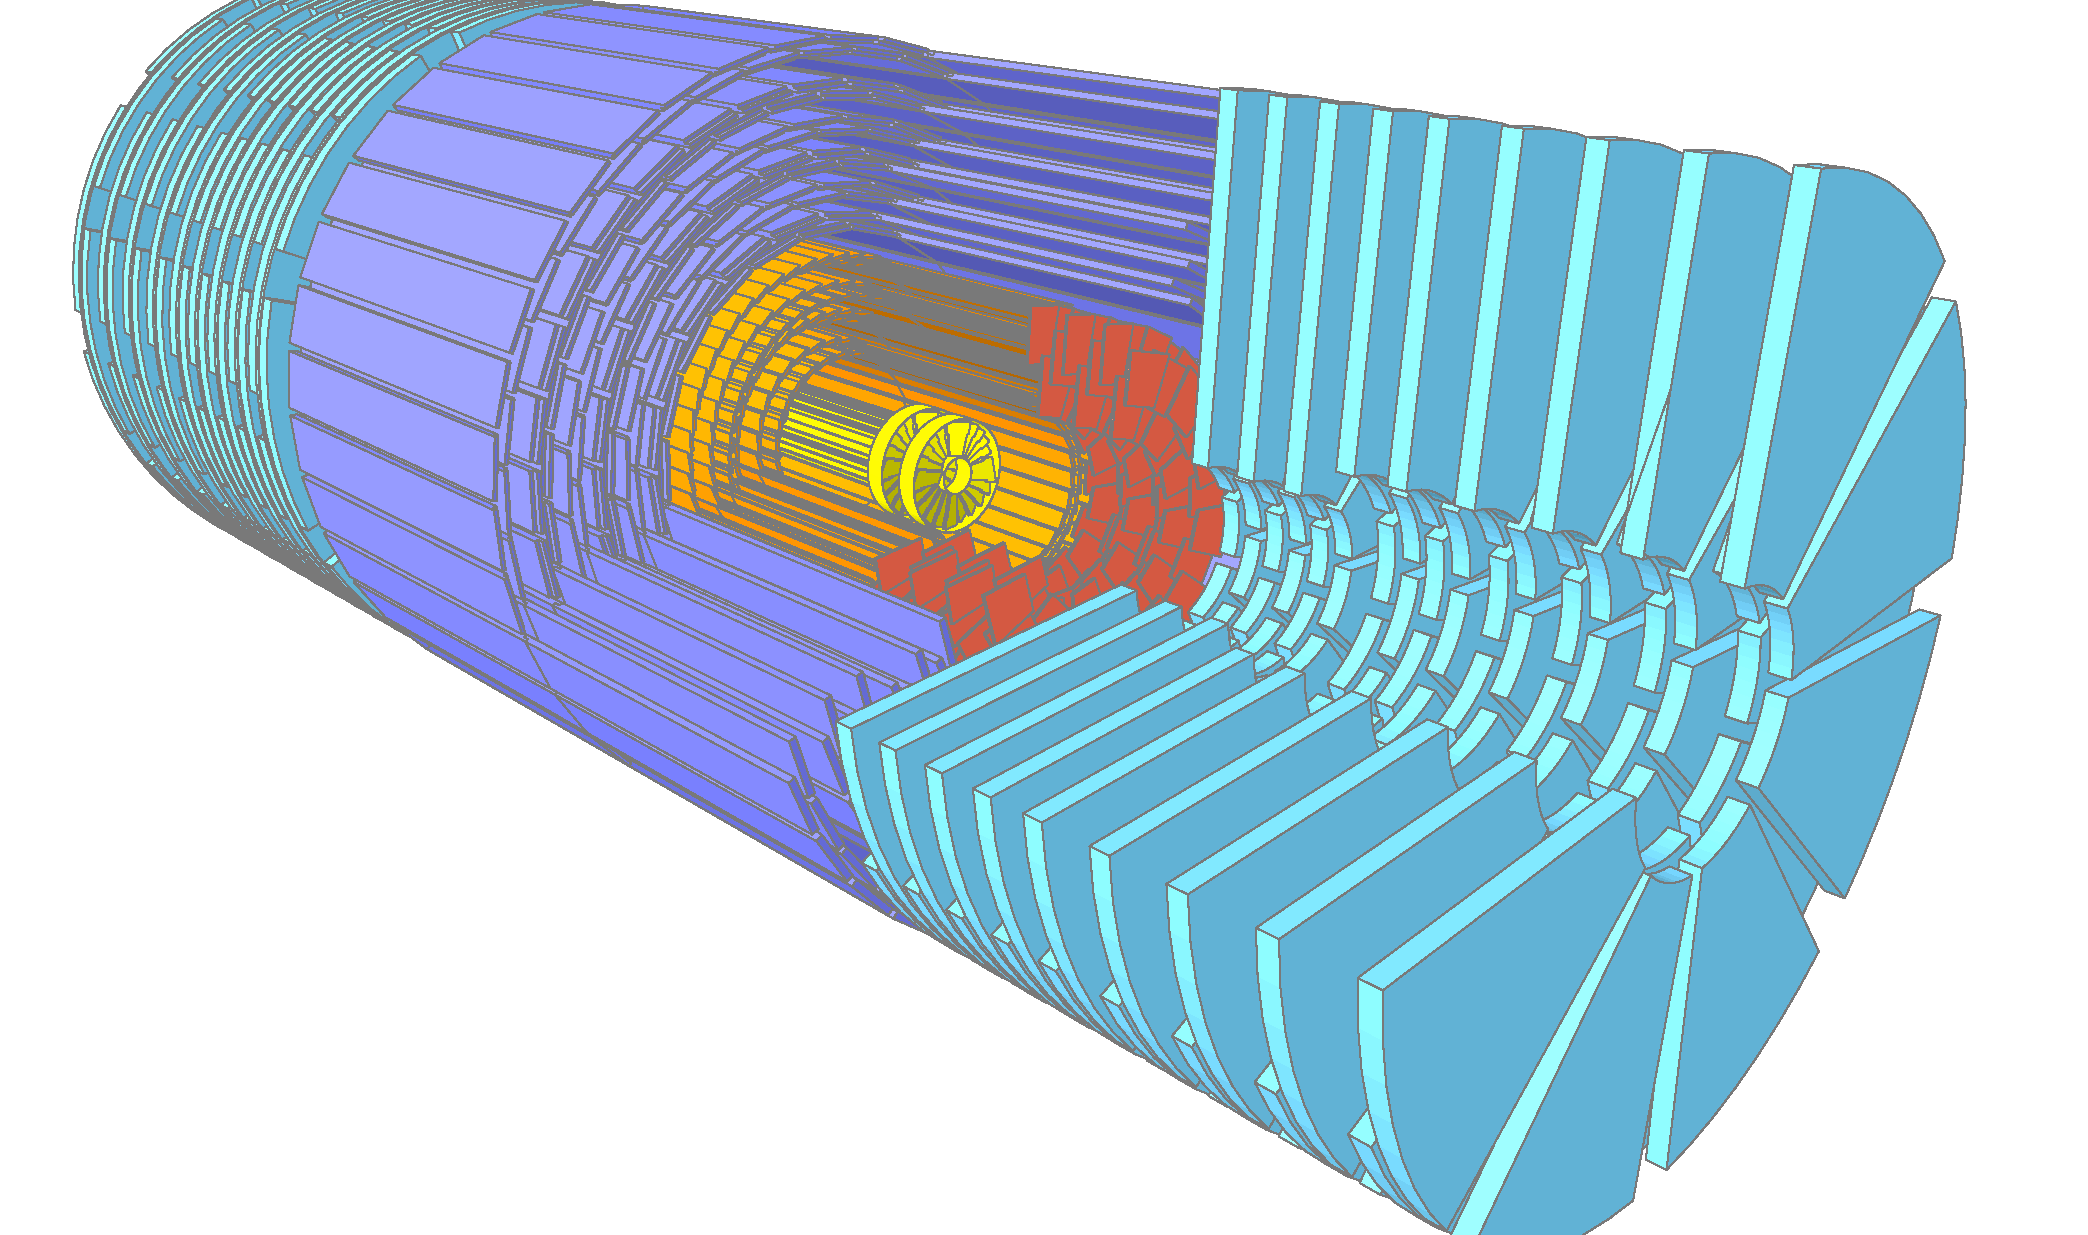
\includegraphics[width=0.6\textwidth]{figures/apparatus/tracker_colour.pdf}
        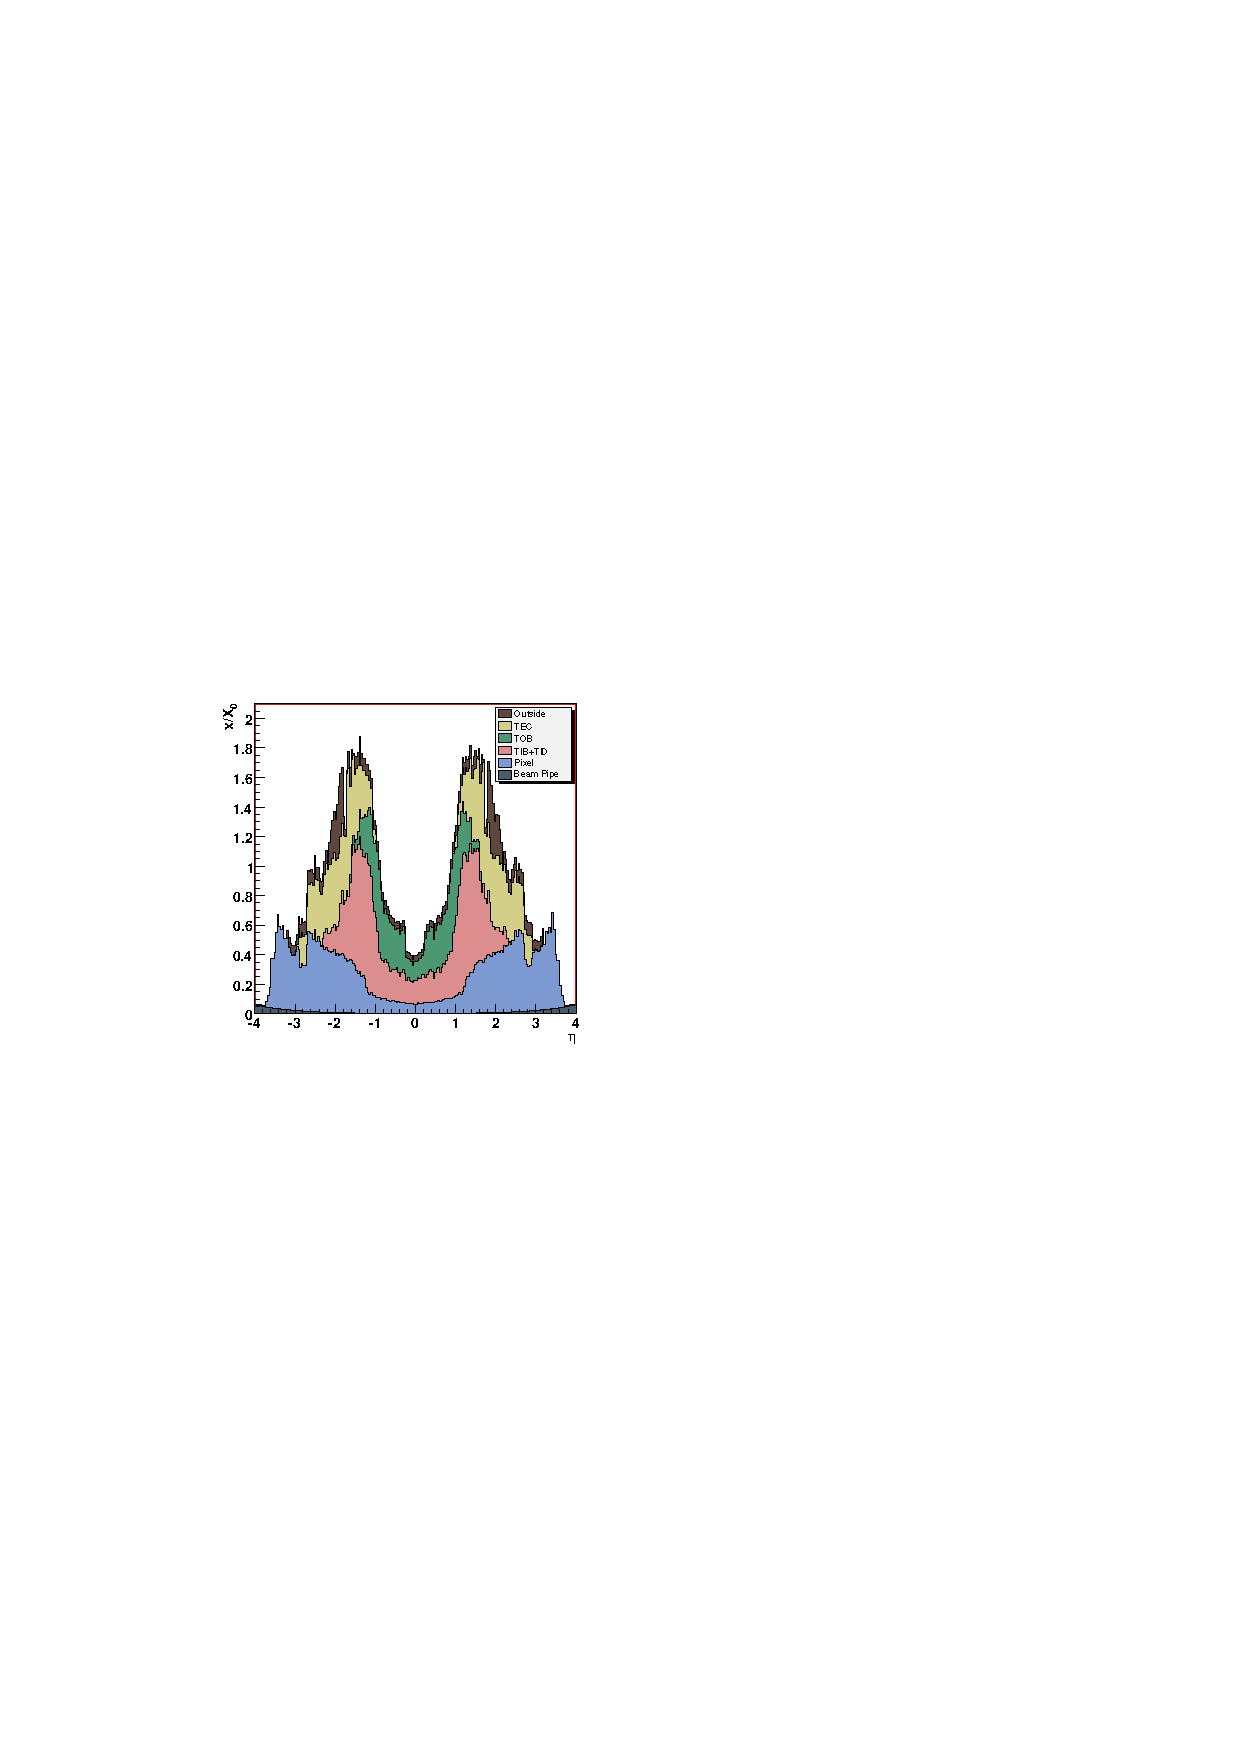
\includegraphics[width=0.39\textwidth]{figures/apparatus/tracker_material.pdf}
    \end{center}
    \caption{Left: the tracker subsystem showing the the central pixel detector in yellow, TIB in orange, TID in red, TOB in purple and TECs in blue \cite{SketchupCMS}. Right: the material before the ECAL in radiation lengths ($X_{0}$) \cite{CMSatLHC}.}
    \label{fig:apparatus:tracker}
\end{figure}
These are assembled into several subsystems: the pixel, the tracker inner barrel (TIB), the tracker inner disks (TID), the tracker outer barrel (TOB) and the tracker endcaps (TEC).

The innermost subsystem of the tracker is the pixel detector which provides precise measurements in $\phi$, $r$ and $z$ of particle trajectories and achieves a high transverse and longitudinal position resolution. The pixel consists of pixel sensors arranged in cylinders of 4.4\,cm, 7.3\,cm, and 10.2\,cm with two disks of pixels sensors at either end to give a total of 66 million pixels and an active area of 1\,m$^{2}$. This gives a pseudorapidity coverage of $|\eta|<2.5$ and at least three position determinations along each track with a transverse resolution of 10\,$\mu$m and longitudinal resolution of 20-40\,$\mu$m. Further out from the pixel detector all of the tracker subsystems use silicon microstrip sensors. 


Situated around the pixel detector are the TIB and TID subsystems which extend in radius out to 55\,cm and consist of four cylinders of sensors in the TIB and three disks of sensors in the TID. These deliver up to four $r$-$\phi$ measurements using sensors oriented parallel to the beam axis in the barrel and radially on the disks. These sensors have a pitch of 80\,$\mu$m in layers one and two of the TIB and 120\,$\mu$m further out giving a position resolution of 23\,$\mu$m and 35\,$\mu$m respectively. 
Surrounding the TIB and TID is the TOB subsystem which has an outer radius of 116\,cm, $z$ between $\pm$118\,cm and consists of six cylindrical layers with pitches of 183\,$\mu$m in the first four layers and 122\,$\mu$m in the fifth and sixth. This gives six $r$-$\phi$ measurements with single point resolutions of 53\,$\mu$m and 35\,$\mu$m respectively. 
Finally, at either end, are the TEC tracker subsystems which extend in radius from 22.5\,cm to 113.5\,cm and extend in $|z|$ between 124\,cm and 282\,cm. Each of the two TECs consist of nine disks of up to seven rings of radially-oriented microstrip sensors. This gives up to nine measurements of $\phi$ for each trajectory.  
Some of the microstrip modules are in pairs to provide a second coordinate measurement: $z$ in the cylindrical layers, $r$ in the discs. They are mounted back to back and rotated by 100\,mrad with respect to each other. These modules make up the first two layers of the TIB and TOB, the first two rings of the TID and the first, second and fifth rings of the TECs.  
All of this ensures $\approx$9 precision measurements of trajectories in the silicon microstrip part of the tracker in the range $|\eta|<2.4$ with $\approx$4 of them being two-dimensional.


The entire tracker material budget manages to remain under two radiation lengths: it ranges from $0.4$\,$X_{0}$ at $|\eta|\approx{0}$ to about $1.8$\,$X_{0}$ at $|\eta|\approx{1.4}$ back to about $1$\,$X_{0}$ at $|\eta|\approx{2.5}$. This is shown in Figure \ref{fig:apparatus:tracker}.


\subsection{Electromagnetic Calorimetry}

The CMS ECAL \cite{CMSEcalTDR} is a calorimeter designed to reconstruct the energy of electromagnetically-interacting particles such as photons with good resolution. In particular the ECAL is aimed at the detection and reconstruction of leptonic and diphoton Higgs final states with good mass resolution within the confines of the CMS solenoid and in LHC operating conditions. To meet these requirements the ECAL must have fine spatial granularity, a large spatial acceptance, a fast response time, and it must capture maximal information from the showers in the restricted space available within the solenoid. 

%\subsubsection{Geometry}
%Overall geometry
The ECAL as a whole has the following geometry (Figure \ref{fig:apparatus:ecal}): the barrel region (EB) covers a pseudorapidity range of $|\eta|<1.442$, there is then a gap between $1.4442<|\eta|<1.566$, and finally the endcaps (EE) cover the range $1.566<|\eta|<3$. Due to prohibitive radiation and pileup conditions electrons and photons are only measured with precision up to $|\eta|<2.5$. 
In addition to these subsystems there is the preshower detector (ES) mounted in front of the endcaps which occupy the range $1.54<|\eta|<2.61$. The ES consist of two disks of lead absorber followed by two planes of silicon strip detectors with pitch $1.9$\,mm. This is used for $\pi_{0}$ rejection. 
\begin{figure}[h!]
    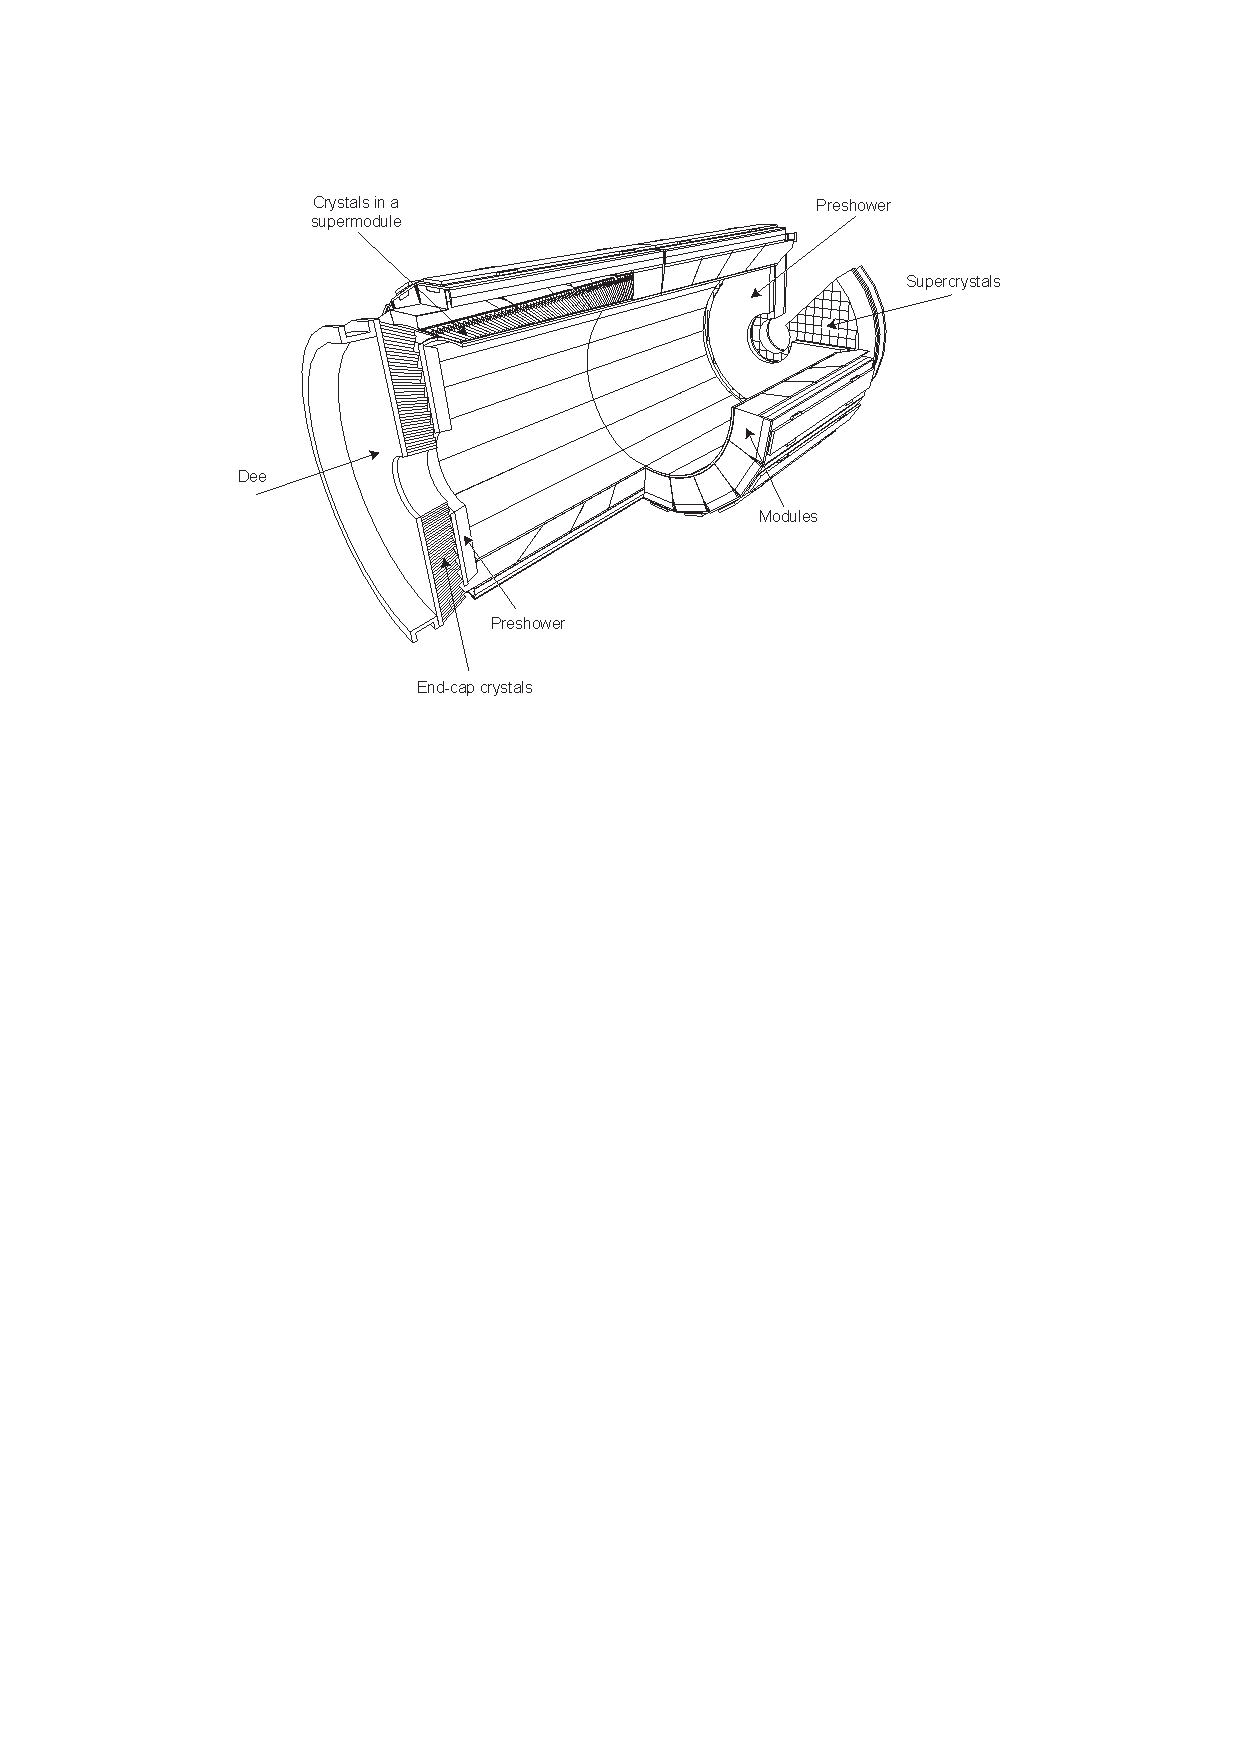
\includegraphics[width=0.9\textwidth]{figures/apparatus/ECAL_alt.pdf}
    \caption{The CMS ECAL with a section removed to show structure \cite{CMSatLHC}.}
    \label{fig:apparatus:ecal}
\end{figure}

%Crystal geometry
The EB and the EE regions are constructed out of lead tungstate (PbWO$_{4}$) crystals, 61200 in the former and 7324 in the latter. The choice of PbWO$_{4}$ was made due to its short radiation length (0.89\,cm), and small Moli\`{e}re radius. The short radiation length ensures that particle showers are shorter in extent and can be contained in as small a depth as possible. The short Moli\`{e}re radius (a measure of showers spread transverse to their direction in a material) ensures that the showers are more contained in the $\eta$,$\phi$ directions. 

%Barrel
In the EB each crystal has a front face of 22x22\,mm$^{2}$ which corresponds to the Moli\`{e}re radius of 21.9\,mm and a segmentation of $(\Delta\eta,\Delta\phi) = (0.0174,0.0174)$. 
The crystals are also tapered in $\eta$ with 25.8\,$X_{0}$ length (230\,mm) and are oriented at a $3^{\circ}$ offset from the average primary vertex position in $\eta$ and $\phi$. This improves the hermeticity.
%Endcap
In the EE the crystals have a front face of $28.6\times{}28.6$\,mm, are 24.7\,$X_{0}$ (220\,mm) in length. 

%Crystal groupings
The individual crystals are grouped together in both the EB and EE. In the EB they are grouped into 36 `supermodules' which cover a $\Delta\phi = 20^{\circ}$ and extend half the barrel length in $z$.
In each EE identically-shaped crystals are grouped into $5\times5$ `supercrystals' arranged in a rectangular $x$-$y$ grid with angular offsets of $2$-$8^{\circ}$.

%\subsubsection{Electronics and trigger}
When a particle enters one of the crystals and then showers scintillation light will be produced and collected by a sensor at the opposite end. This sensor will produce a pulse which is amplified and then converted into a digital signal. The height of this digitised pulse is then used to determine the energy deposition within the crystal. 
Two different types of sensor are used: in the barrel region avalanche photodiodes are used, the endcaps vacuum phototriodes are used due to the different magnetic field properties and higher radiation levels.
Crystals are read out as $5\times{5}$ trigger towers whose digital signal sum constitutes the fast, coarse information provided to the trigger system with every bunch crossing.


%\subsubsection{Calibration and performance}

The energy resolution of a single PbWO$_{4}$ crystal is modelled with the following equation \cite{CMSPhysics}
\begin{equation}
    \label{eq:apparatus:ecal_energy_reso}
        \left( \frac{\sigma}{E} \right)^{2} =  
        \left( \frac{S}{\sqrt{E}} \right)^{2} +  
        \left( \frac{N}{E} \right)^{2} +  
        C^{2},
\end{equation}
where $S$ is the stochastic term, $N$ is a noise term, and $C$ is a constant term. The crystal performance was measured in a test beam and the above parameters determined by fitting a Gaussian function to the reconstructed energy distributions. Their values were measured to be $S=2.8$\,GeV$^{\frac{1}{2}}$, $N=0.12$\,GeV, and $C=0.3$\%.

To reconstruct the energy of a photon or electron, multiple crystals are typically used as the shower spreads in the ECAL, or even starts before it reaches it. 
Clustering algorithms \cite{ecalShower} are used to reconstruct energy from these crystals and assemble them into a supercluster (SC). The energy associated to the supercluster is then calculated as
\begin{equation}
    E_{SC} = F_{SC}G\sum^{N_{c}}_{i=0}A_{i}C_{i}S_{i}(t)
\end{equation}
where $N_{c}$ is the number of crystals in the SC, $A_{i}$ is the amplitude of the pulse of crystal $i$, $S_{i}(t)$ corrects crystal transparency loss due to radiation, $C_{i}$ is a factor that adjusts the response of the crystal, $G$ is a conversion factor from the digital signal to GeV (global energy scale) and $F_{SC}$ is a correction to the SC energy sum due to second order effects.

To calibrate the ECAL \cite{cmsEcalCalibration} one must use a variety of measurements to determine the factors $G$, $C_{i}$, and $S_{i}(t)$ which correspond to calibration of the overall energy scale, uniformity of measurement in space and uniformity over time respectively. 
Corrections over time due to radiation-induced transparency change in the crystals ($S_{i}(t)$) are derived by injecting laser light at 440\,nm every 40 minutes. 

Several methods are used to derive the factors for an even crystal response over the ECAL spatial extent which use the symmetries of CMS. Firstly one uses $\phi$ symmetry to find factors in rings of $\eta$ which should all have the same response. 
Other methods reconstruct particles of known mass decaying to diphotons and use this as a standard candle. The mass should be the same in each part of the detector which allows for the determination of regional differences in response. These different methods are combined to give a collection of per-crystal corrections. 

The final factor, the global energy scale, is derived by reconstructing Z bosons which have decayed to an $e^{+}$,$e^{-}$ pair and comparing the measured mass to the known value














\subsection{Hadron Calorimetry}
The CMS HCAL \cite{cmsHcal} is situated around the ECAL and its function is to identify neutral hadrons, measure their energies and positions, and to determine $E_{T}^{\mathrm{miss}}$ at good resolution over a large acceptance.
It is a sampling calorimeter which uses material to produce particle showers (absorber) which is distinct from the active material measuring deposited energy, unlike the ECAL which is a homogeneous calorimeter where one material (lead tungstate) performs both functions. 

The structure of the HCAL is shown in Figure \ref{fig:apparatus:hcal}. It consists of a barrel region (HB), two endcaps (HE), a region outside the solenoid (HO), and two forward calorimeters (HF) which take the HCAL acceptance up to $|\eta|<5$. 
\begin{figure}[h!]
    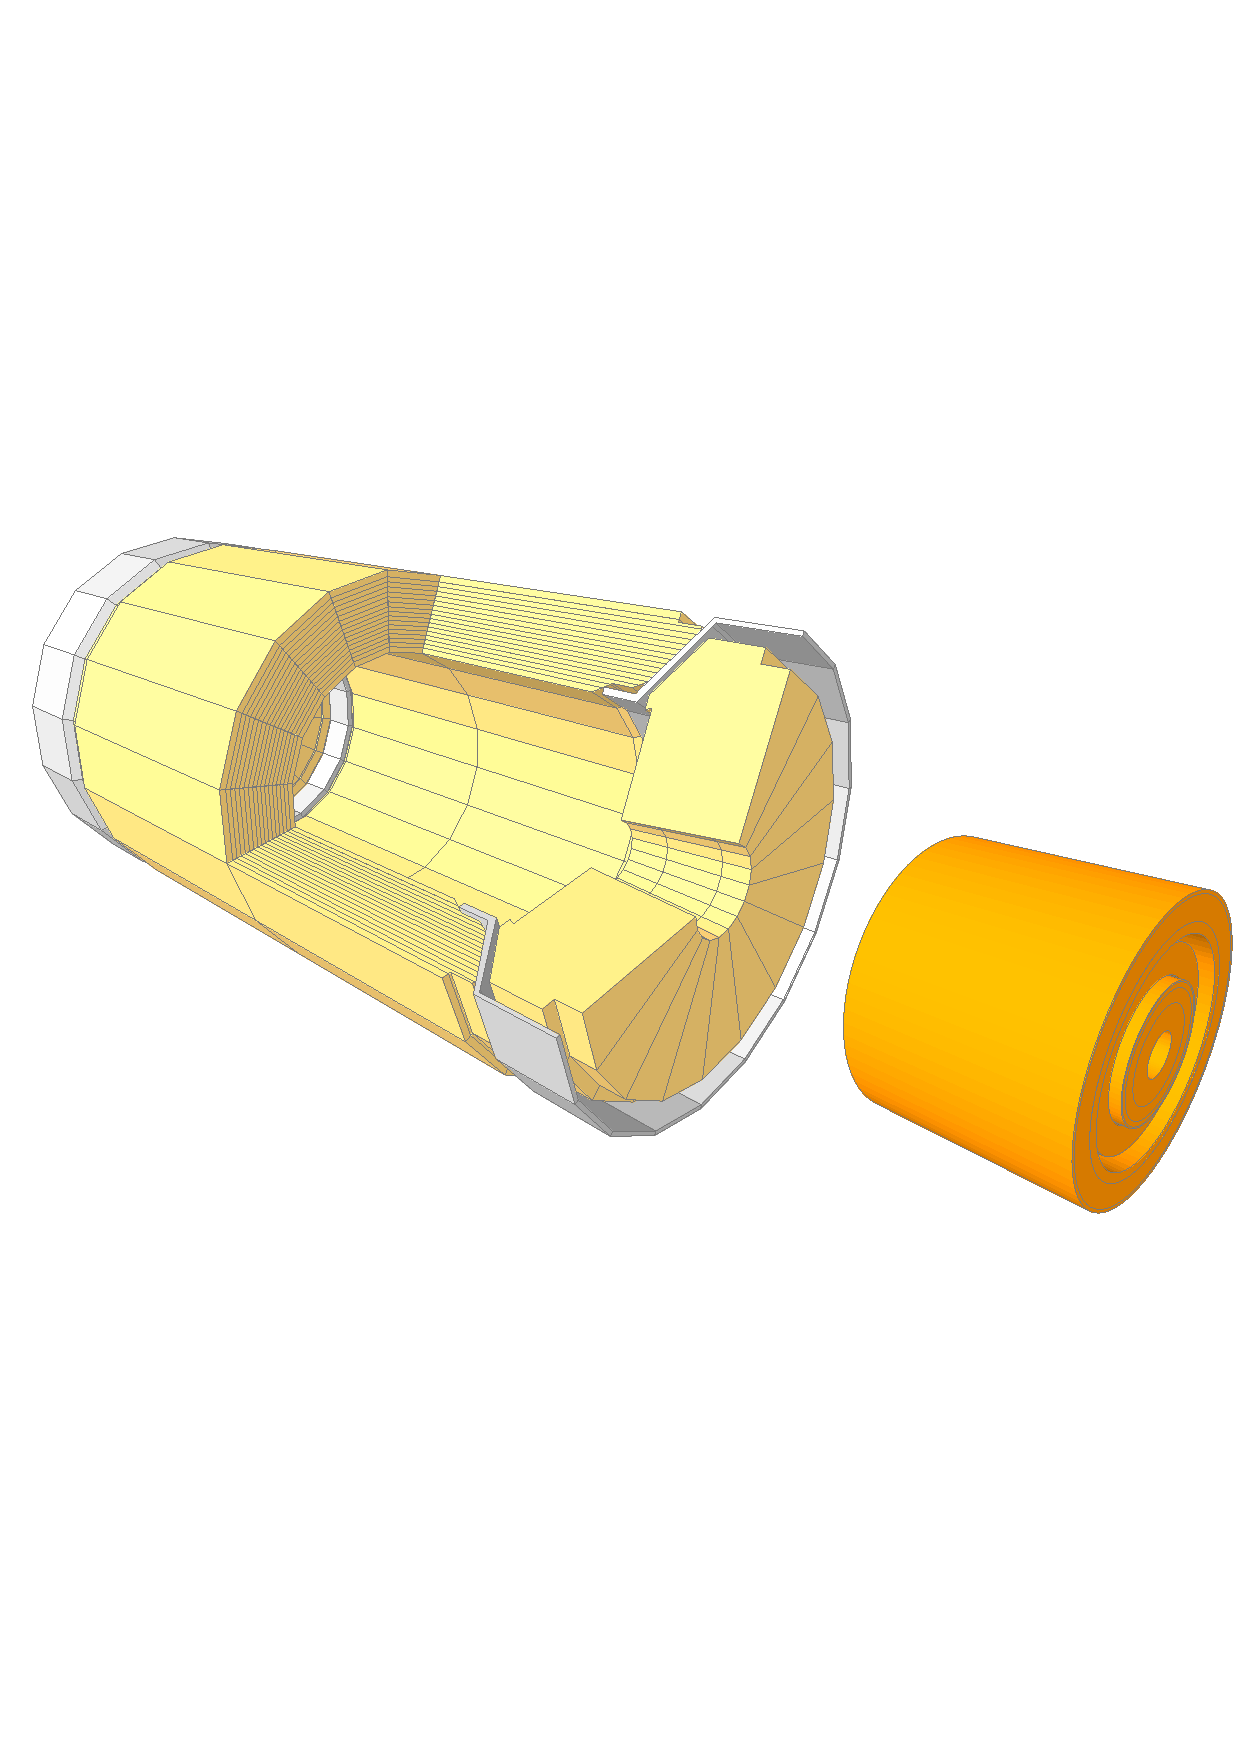
\includegraphics[width=0.9\textwidth]{figures/apparatus/HCAL_HF.pdf}
    \caption{The CMS HCAL with the barrel and endcap sections (left) with part removed to show structure and the forward hadronic calorimeter (right) \cite{SketchupCMS}.}
    \label{fig:apparatus:hcal}
\end{figure}
The HB region covers a pseudorapidity range of $|\eta|<1.3$ and consists of two half-barrel sections that slot in to either end of the solenoid bore each of which consist of 36 identical wedges in the azimuthal angle $\phi$. These wedges are constructed from 2 steel and 14 brass absorber plates with a plastic scintillator active material in alternating layers. Brass is used because it is non-magnetic, steel absorber is only used in the innermost and outermost plates to provide structural support. Each wedge is segmented into four azimuthal regions and the plastic scintillator is divided into 16 pseudorapididty regions giving a granularity of $(\Delta\eta,\Delta\phi) = (0.087,0.087)$.
The HE regions cover a pseudorapidity range $1.3<|\eta|<3$ and is divided into 36 azimuthal wedges. It uses brass absorber plates and achieves a granularity between $(\Delta\eta,\Delta\phi) = (0.087,0.087)$ and $(0.017,0.017)$
The HF region covers a pseudorapidity range from $3<|\eta|<5$ and must deal with extremely high levels of radiation. This motivates a different construction with quartz fibres chosen for the active material and steel for the absorber. It is cylindrical in structure with 5\,mm thick grooved plates where the fibres fit into the grooves and operate by detecting Cherenkov light produced by incident particles. The fibres are bundled to form $(\Delta\eta,\Delta\phi) = (0.175,0.175)$ towers.
Finally, the HO covers the barrel region around the solenoid and consists of plastic scintillator tiles which follow the granularity of the HB. It uses the solenoid itself as the absorber and is designed to operate as a shower `tail catcher' which compensates for hadron showers that begin later in the HCAL and may not be properly measured. This leakage has a direct effect on the measurement of $E_{T}^{\mathrm{miss}}$.



\subsection{Muon Detection}

The CMS muon system \cite{cmsMuon} is situated around the outside of the solenoid and consists of detectors interleaved with the steel return yoke assembled into barrel and endcap regions (Figure \ref{fig:apparatus:muon}).
The muon system has three objectives: to identify muons, to measure their momentum with precision, and to trigger on them over a large spatial acceptance. 
\begin{figure}[h!]
    \begin{center}
        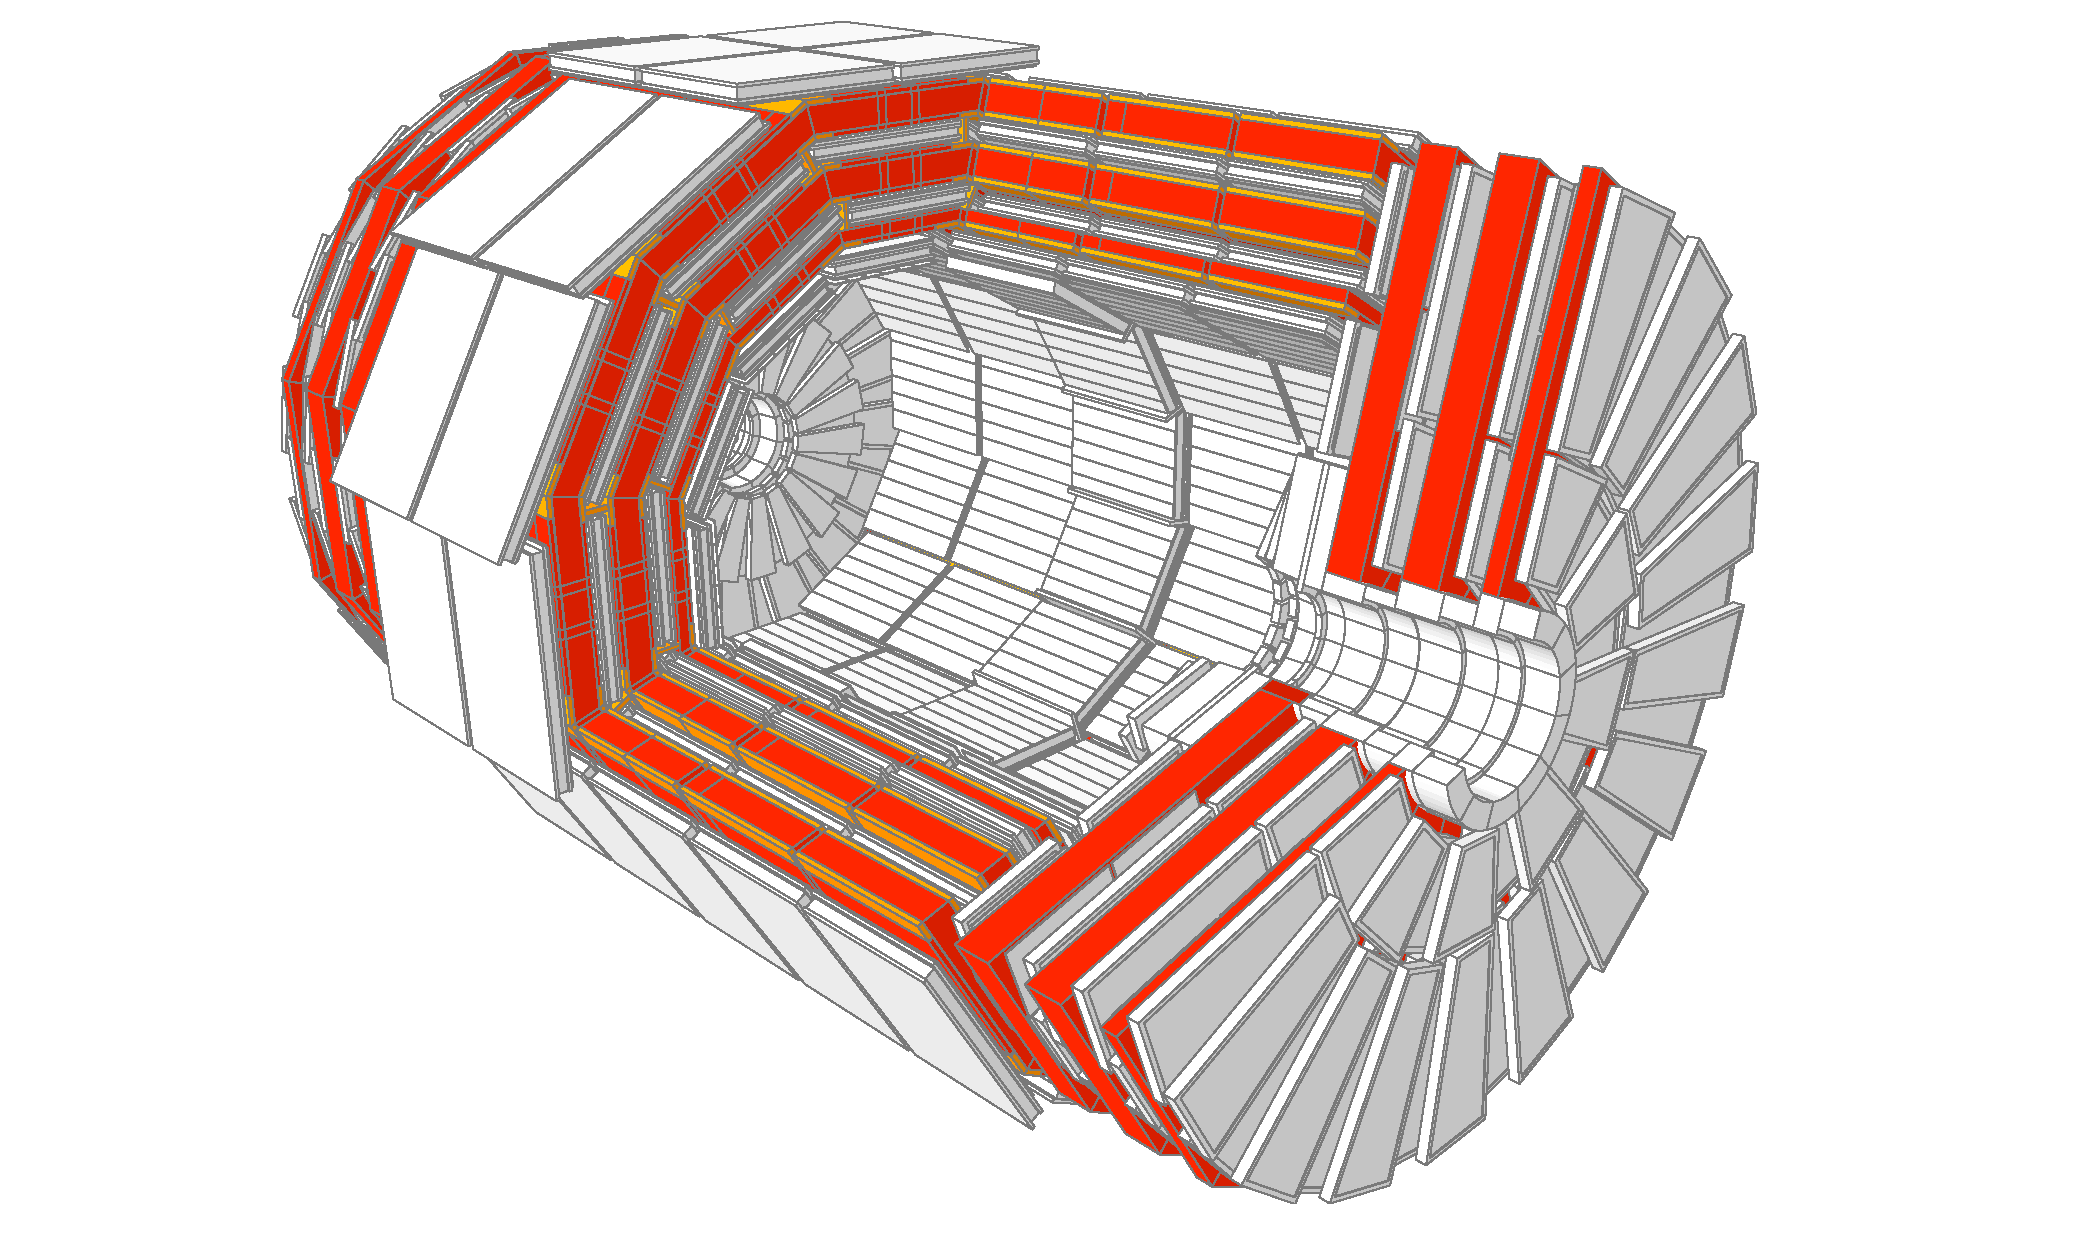
\includegraphics[width=0.49\textwidth]{figures/apparatus/MUON.pdf}
        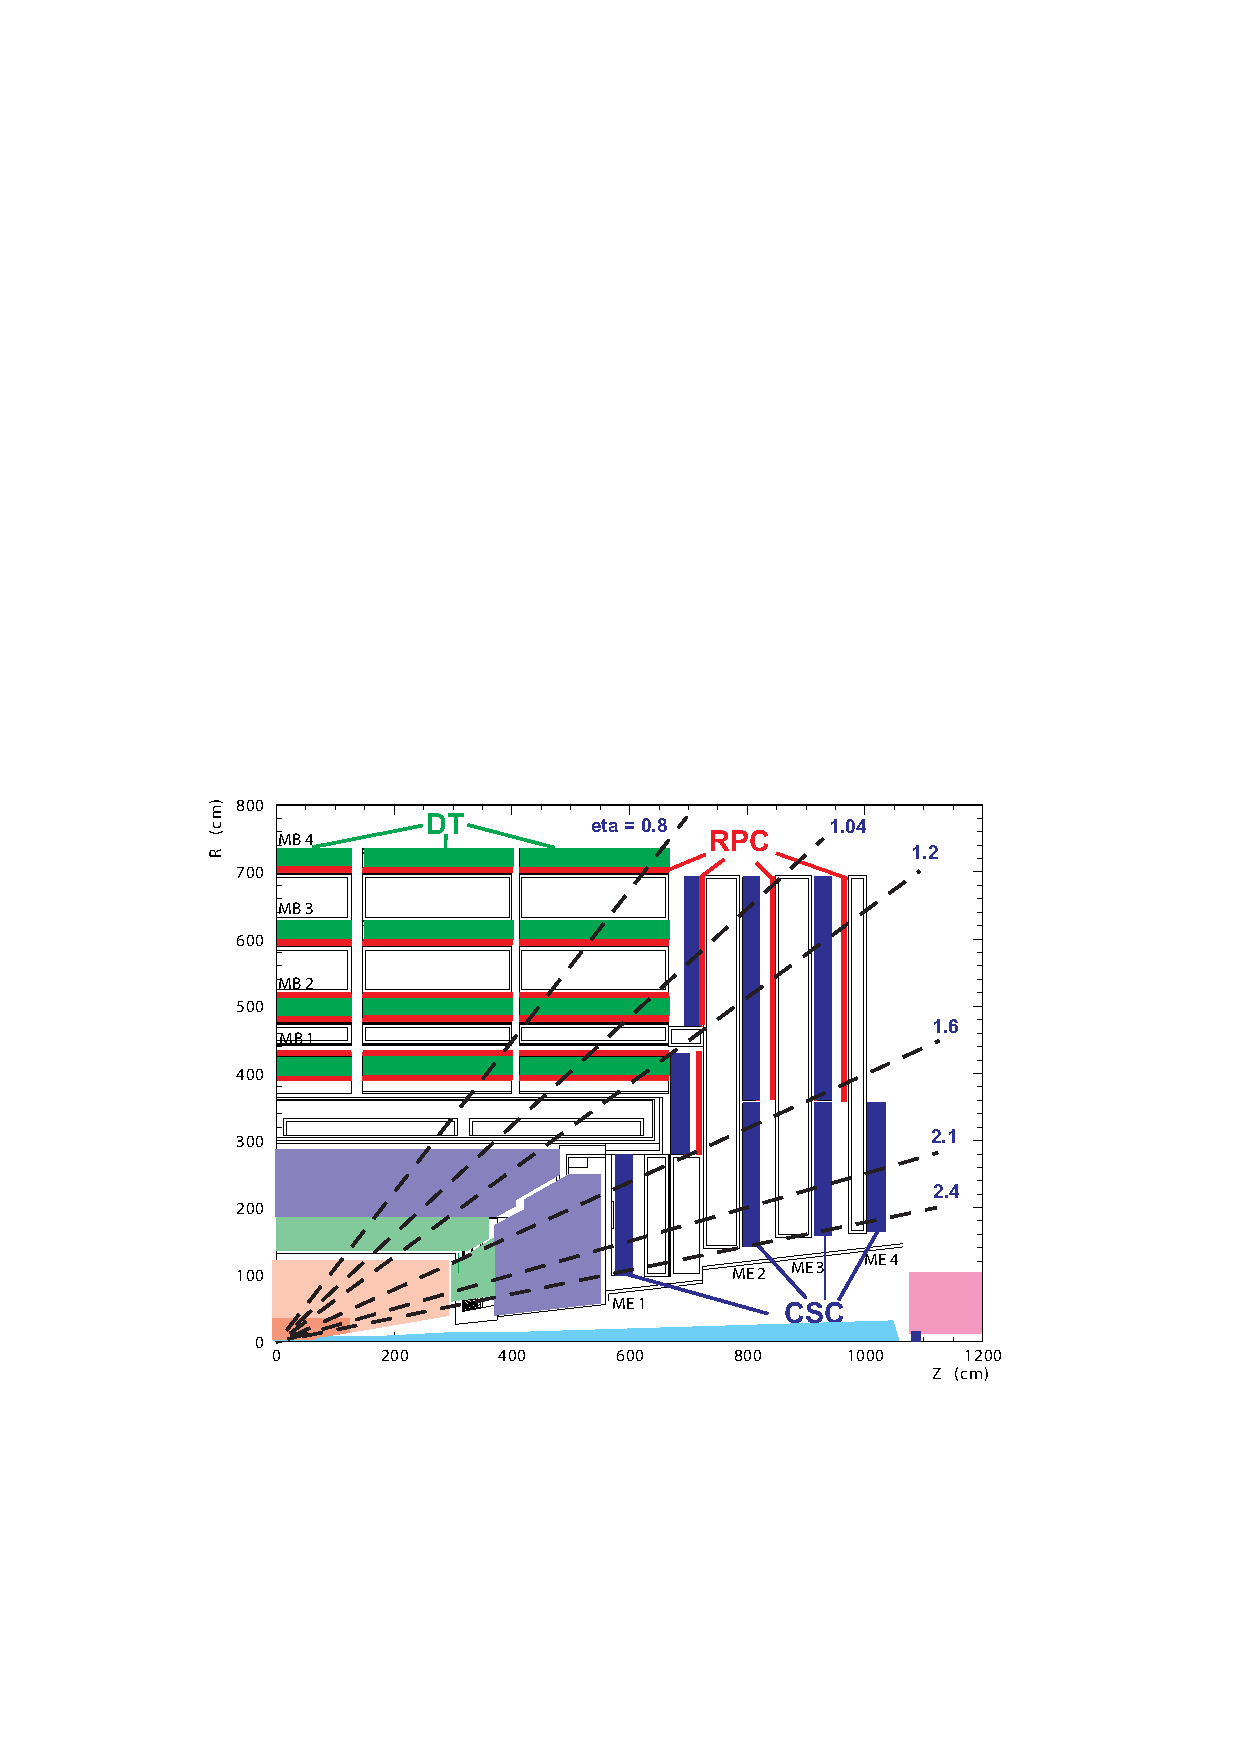
\includegraphics[width=0.49\textwidth]{figures/apparatus/muon_diagram.pdf}
    \end{center}
    \caption{Left: the CMS muon detector subsystems (white) within the structure of the steel return yoke (red) \cite{SketchupCMS}. Right: a diagram showing a quarter-view of of the muon system with detector types labelled.}
    \label{fig:apparatus:muon}
\end{figure}
The muon detectors are all gas-based and belong to three different types: drift tubes (DTs), cathode strip chambers (CSCs) and reactive plate chambers (RPCs). They all operate the same way, with incident particles ionising gas, producing free electrons which drift towards the anode and produce an electrical signal. 

In the barrel region DTs are used as the magnetic field is more uniform, the neutron flux is small and the muon rate is lower. They are arranged in four layers covering the pseudrorapidity $|\eta|<1.2$ where the detectors in the first three layers have a different construction to the fourth. First three layers' detectors consist of 8 chambers in 2 groups of 4: the first half measure in the $r$-$\phi$ plane, the second half measure in $z$. The outermost detectors do not have the $z$ determination. All of these detectors use aluminium wires with an Ar plus CO$_{2}$ gas mix and achieve a position resolution of 100\,$\mu$m.


In the endcap regions the magnetic field is less uniform, the neutron-induced background is high and so is the muon rate. This lead to the adoption of CSC technology due to their fast timing ability, granularity, and robustness to high radiation. 
These detectors cover a pseudorapidity region of $0.9<|\eta|<2.4$ and are arranged in four layers. Each detector consists of 6 gas gaps with cathode strips running radially away from the beamline and anode wires running perpendicularly to the cathode strips. The cathode strips give a precise but relatively slow measurement in the $r$-$\phi$ plane and the anodes measure in $\eta$ with fast timing for triggering and bunch crossing attribution. They achieve a position resolution of around 200\,$\mu$m. 


Finally, in addition to the DTs and CSCs, the muon system uses RPCs placed in the barrel and the endcaps (up to $|\eta|<1.6$) as an independent and complimentary way of triggering. 
RPCs are double gap chambers which operate in avalanche mode to give a fast response time and good timing resolution. In the barrel region there are six layers of RPCs: two layers in each of the first two layers of drift tubes and one each in the last two. This redundancy helps with triggering on muons with low-$p_{T}$. In the endcaps there are planes of RPCs in each of the layers which, in addition to triggering, help to resolve ambiguities in the CSCs when there are multiple tracks in a chamber. 


\subsection{Trigger system and Storage}
The LHC delivered bunch crossings to CMS at a rate of 40\,MHz in the 2016 period. With each of these events requiring up to 1MB of memory this would amount 40\,TB per second of readout and storage which is not feasible. 
However, most of these events are not physically interesting: they will mostly be low-energy interactions where the protons only glance off each other rather than collide head-on. 

To filter these events a fast measurement and decision must be made whether to store or discard, this is achieved with the CMS trigger system \cite{trigger}. The trigger system operates as a two-step process: first the hardware-based level-1 trigger (L1T) makes fast decisions on whether to keep events using coarse information from some of the subsystems; and then the software-based high-level trigger (HLT) cuts the rate further by using all detector subsystems and a basic physics object reconstruction. 


The L1T achieves a rate reduction of 40\,MHz to 100\,kHz by performing fast calculations using custom, reprogrammable hardware called field-programmable gate arrays (FPGAs).
To achieve this the L1T must make an accept decision within 3.2\,$\mu$s which includes time of transmission from the detector and decision return. 
Coarse information is received from the ECAL, HCAL, and the muon system due to speed and bandwidth limitations and stored in a buffer which contains information from multiple bunch crossings. 
Furthermore there is insufficient time for using correlations between subdetectors and also insufficient time and other resources to use information from the tracker. 
Once information is received, a collection of algorithms are used to pick out relevant events and if the event is accepted the entire detector readout is passed on to the HLT.


At the HLT the data rate is still too high and must be cut further to 1\,kHz. This is achieved with a computing farm a short distance away from the CMS detector which runs a basic reconstruction of physics objects from the full CMS readout including the tracker. Here more sophisticated algorithms may be run to pick out collections of objects in events and make the final accept decision.
After this events are recorded to permanent storage, put through the full CMS reconstruction, evaluated for data quality and then made available to physics analyses. 







    \chapter{Machine Learning}
\label{chap:machine_learning}


\newpage

The field of Machine Learning (ML) is concerned with algorithms which can be said to `learn' from experience, this may be contrasted with algorithms which achieve some task with a set of static instructions. The ability to learn allows ML algorithms to solve problems which may be too complex for a collection of explicity defined instructions. 
This chapter will give an overview of machine learning as relevant to the Higgs diphoton decay analysis at CMS and as a result certain definitions will not be as general. 

\section{Machine Learning Fundamentals}

A formal definition of learning is given in (ref): an algorithm is said to \textit{``learn from experience $E$ with respect to some class of tasks $T$ and performance measure $P$, if its performance at tasks in $T$, as measured by $P$, improves with experience $E$''}. 
The task $T$ may be defined in terms of the `features' of individual members of the dataset at what one is trying to achieve with them and these are typically represented as a vector $\vec{x}\in\mathbb{R}^{n}$ where each element of the vector is a feature of the datapoint. The two main classes of tasks we are interested in are classification and regression:
\begin{itemize}[leftmargin=.5in,noitemsep]
    \item Classification:
    \item Regression:
\end{itemize}



    \chapter{Object Reconstruction and Selection}
\label{chap:object_reco}

\newpage

\section{Introduction}

%High-level overview
The CMS $H\rightarrow{\gamma\gamma}$ analysis works by searching for excess production in the distribution of diphoton invariant masses. A Higgs boson signal will manifest as a small bump on top of a continuous distribution due to background processes from Standard Model diphoton production.

The invariant mass of a diphoton system is calculated with the expression
\begin{equation}
    m_{\gamma\gamma} = \sqrt{2E_{\gamma_1}E_{\gamma_2}(1-\cos{\alpha})},
\end{equation}
where $E_{\gamma_1}$ and $E_{\gamma_2}$ are the energies of the leading energy photon and subleading energy photon respectively, and $\alpha$ is the opening angle between them. 
To determine the value of $\alpha$ we require the locations of the photons in the ECAL and the correct originating vertex. 
Good identification and measurement of photons and their verices are therefore crucial to the analysis, and the reconstruction of these will be described in detail in this chapter. 
Other objects such as jets and leptons provide extra information on signal events and allow for improved signal isolation. The reconstruction of these objects will also be described.

\section{ECAL Clusters and Particles}

ECAL clusters are used in many of the object of interest in this chapter and are especially important for photons. 
The clustering \cite{cmsEcalCalibration} begins with the identification of local energy maxima above a threshold value, these are referred to as seeds. 
After this topological clusters are grown from the seeds by gathering crystals which share at least one side with a seed, or crystals clustered with a seed, with energy above another threshold which is equal to $2\sigma$ of the ECAL electronic noise (up to 80\,MeV in the barrel and 300\,MeV in the endcaps).
Finally, these clusters are merged to form superclusters which allow for good energy containment, accounting for variation in the construction of the ECAL with $|\eta|$, and pileup robustness.



Physics objects are reconstructed with the CMS global event description known as particle flow (PF) \cite{ParticleFlow}.
PF uses information from all of the subdetectors to identify and reconstruct individual particles produced within CMS, and to achieve good energy resolution.
The information used as inputs are tracks from the tracker, tracks from the muon systems, and energy clusters from the ECAL and HCAL. Depending on which of these are present, PF will output `PF candidates' which correspond to different types of semi-stable particles 
\begin{itemize}[leftmargin=.5in,noitemsep]
    \item Photons: ECAL deposition is present with no associated track in tracker. The energy of photons is obtained from the ECAL. 
    \item Electrons: ECAL supercluster is present with associated track in tracker. Energy is determined with electron momentum at the primary vertex, the ECAL deposition, and the energy of associated Bremsstrahlung photons. 
    \item Muons: compatible tracks in tracker and muon system. Energy is determined from the curvature or the tracks. 
    \item Charged Hadrons: track in tracker, ECAL deposition and associated HCAL deposition. Energy is determined from the track curvature, and the matching ECAL/HCAL deposits corrected for effects from zero-suppression and for the response of the calorimeters to hadronic showers.
    \item Neutral Hadrons: measured with the corrected energies from the ECAL and HCAL. 
\end{itemize}
These PF candidates are then used to construct jets, and to determine missing transverse momentum $p_{T}^{miss}$.
This process is applied in the same way to data collected with the CMS detector and data from simulation.


\section{Samples}

\subsection{Trigger}
The analysis uses events selected with the two-step CMS triggering system (L1T and HLT). The objective of this system is to keep the event rate below an acceptable level due to limited bandwidth resources, whilst keeping signal efficiency a high as possible. Requirements at L1T are looser because it uses fast coarse measurement, HLT uses more stringent requirements to compensate for any inefficiencies from this. 

At L1T we require one or two energy deposits in the ECAL with energy thresholds that varied over the 2016 running period. For the single deposit, energy requirements are more stringent at 25\,GeV during low luminosity up to 40\,GeV at high-luminosity periods to keep the trigger rate to an acceptable level. For two deposits at high-luminosity 22\,GeV and 15\,GeV were required. 

At HLT events were selected with $E_{T}$ thresholds of 30\,GeV and 18\,GeV for the leading and subleading photon respectively. Furthermore, the selection has loose requirements on the shape of the electromagnetic showers, isolation variables, and the ratio of deposition in the ECAL compared to the HCAL. 

These selections have their efficiencies measured with the `tag-and-probe' technique \cite{TagAndProbe}. 
This uses the resonant production and decay to pairs of well-understood particles near their mass peak to ensure a pure and well-understood sample. 
In the $H\rightarrow{\gamma\gamma}$ analysis $Z\rightarrow{}e^{+}e^{-}$ is used as both electrons and photons are reconstructed with the ECAL clustering, so one can use di-electron decays as a proxy for diphotons. 
A strict ID requirement is placed on one of the decay products (the tag) and a looser requirement is placed on the other (the probe). 
The requirement on the probe should be loose enough that it does not affect the selection being measured. The selection efficiency may then be measured as the proportion of the probes which satisfy the selection.
%Ref for tag and probe from the PAS


\subsection{Data}
The data used in the analysis corresponds to the 35.9\,fb$^{-1}$ of proton-proton collision data recorded by the CMS experiment in the 2016 run period with a centre of mass energy of $s=\sqrt{13}$\,TeV and selected with the trigger requirements described above. 



\subsection{Simulation}

Simulated samples are used for a variety of tasks such as to train the ML models of the analysis, to optimise cuts and categorisations, producing signal models, and to perform validations. 

Signal events are simulated for a range of mass points from 120\,GeV to 130\,GeV using cross-sections and branching ratios recommended by the LHC cross-section working group. 
The signal events are generated at next-to-leading order in perturbative QCD with \texttt{MadGraph5_{}aMC@NLO}, with  parton showers and hadronization modelled with \texttt{pythia8}. The \texttt{pythia} tune parameter set \texttt{CUETP8M1} is used.

The background simulations are generated in different ways. For the main irreducible background from prompt diphotons \texttt{Sherpa} is used which includes Born processes with up to three jets as well as box diagram processes at leading order. 
For the $\gamma$-jet and jet-jet reducible backgrounds where jets are mistakenly reconstructed as photons we use \texttt{pythia8} with a filter applied to enhance the electromagnetic energy content of the jets. 
Finally, samples for validation $W\gamma$ and $Z\gamma$ are simulated with \texttt{Madgraph} and Drell-Yan (DY) is simulated with \texttt{Madgraph_{}aMC@NLO}


The CMS detector itself is simulated in detail with \texttt{GEANT4}. 
This includes the simulation of both in-time and out-of-time pileup. 
Simulated events are then weighted such that they reproduce the pileup distribution observed in data from CMS.






\section{Vertex Reconstruction}
If the selected vertex is within $1$\,cm of the correct vertex the contribution of spatial uncertainty to the mass resolution is negligible and is dominated by the energy resolution of the CMS ECAL. 
The ECAL gives a good determination of the photon location in $z$ and $\phi$, but it does not provide any pointing information: to determine $\alpha$ precisely we need to determine the correct vertex by other means.
When diphotons are produced in proton collisions there are also charged tracks present from jets or from the proton remnants which are associated to the same vertex. One can exploit this information to choose the correct vertex.  


The process begins by gathering the tracks in the central tracker and grouping them by their common points of origin. These are the candidate vertices. The next step will be to choose the vertex most compatible with the candidate diphoton under consideration.

\subsection{Vertex Selection}
Vertex selection is performed with a BDT classifier which takes a set of input features formed from the transverse momenta of tracks associated to the candidate vertex and the candidate diphoton. The features are
\begin{gather*}
    \sum_{i}|\vec{p}_{T}^{i}|^{2}. \\
    -\sum_{i}(\vec{p}_{T}^{i}\cdot\frac{\vec{p}_{T}^{\gamma\gamma}}{|\vec{p}_{T}^{\gamma\gamma}|}), \\
    (|\sum_{i}\vec{p}_{T}^{i}|-\vec{p}_{T}^{\gamma\gamma})/(|\sum_{i}\vec{p}_{T}^{i}|+\vec{p}_{T}^{\gamma\gamma}),
\end{gather*}
where $i$ enumerates the tracks of the candidate vertex. In the case of converted photons there are two additional features: the number of conversions and the pull $|z_{vtx} - z_{conv}|/\sigma_{z}$ where $z_{vtx}$ is the $z$ position from the vertex, $z_{conv}$ is the position estimated from the conversion tracks, and $\sigma_z$ is the uncertainty on $z_{conv}$.
The BDT is trained on vertices from simulated Higgs boson diphoton events with vertices which correspond to the true Higgs vertex considered the signal class and all others background. The selected vertex is then the candidate with the highest BDT score. 


\subsection{Vertex Probability}
Once a candidate vertex is selected, another BDT is used to score the probability that it is within $1$\,cm of the true vertex location.   
This is also trained on simulated Higgs diphoton events and is given the following input features,
\begin{itemize}[leftmargin=.5in,noitemsep]
    \item The number of vertices in the event.
    \item The three highest vertex ID scores.
    \item $p_{T}$ of the candidate diphoton.
    \item $\Delta{z}$ between the highest scoring vertex and the second highest.
    \item $\Delta{z}$ between the highest scoring vertex and the third highest.
    \item The number of converted photons.
\end{itemize}


\subsection{Performance}
Performance of the vertex selection BDT is validated with both simulated and real $Z\rightarrow{}\mu^{+}\mu^{-}$ events where the muon tracks have been removed and the event re-reconstructed to imitate a diphoton system. 
In the converted-photon case a similar procedure uses $\gamma + $jet events where the vertex is found using the tracks of the jet. 
The tracks of the jet are then removed and the event is re-reconstructed as a diphoton systems. Validation of unconverted photons is shown in Figure \ref{fig:object_reco:vertex_id_valid}. 
\begin{figure}[h!]
    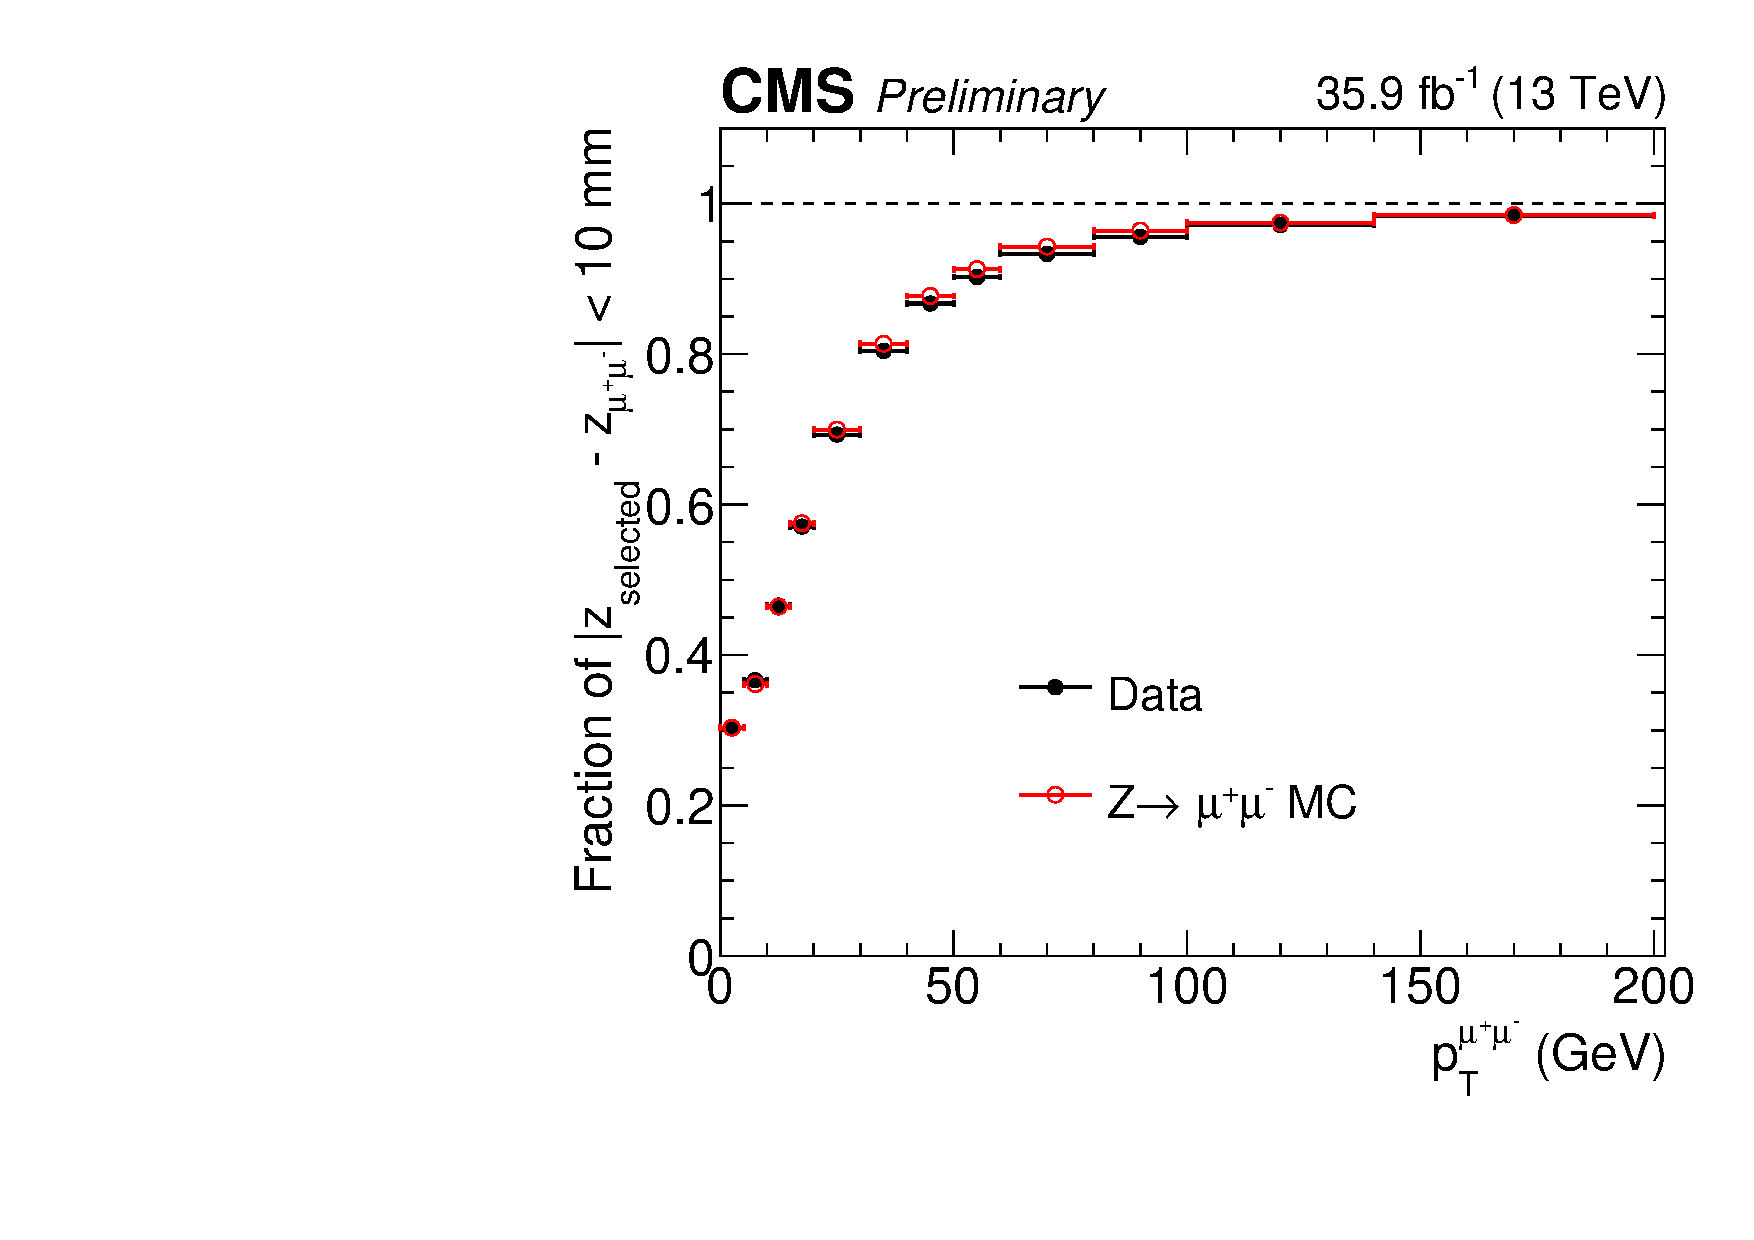
\includegraphics[width=0.45\textwidth]{figures/object_reco/CMS-PAS-HIG-16-040_Figure_003.pdf}
    \caption{Validation of vertex ID. Vertex ID efficiency in simulation and data for dimuon event reconstructed as diphotons.}
        \label{fig:object_reco:vertex_id_valid}
\end{figure}

The selection efficiency for selecting a vertex within $1$\,cm of the true position is evaluated using simulated Higgs diphoton decay events. This efficiency is shown for different bins of number of vertices in the event and the diphoton $p_{T}$ in Figure \ref{fig:object_reco:vertex_id_efficiency}. The efficiency over all events is approximately 81\%.
\begin{figure}[h!]
    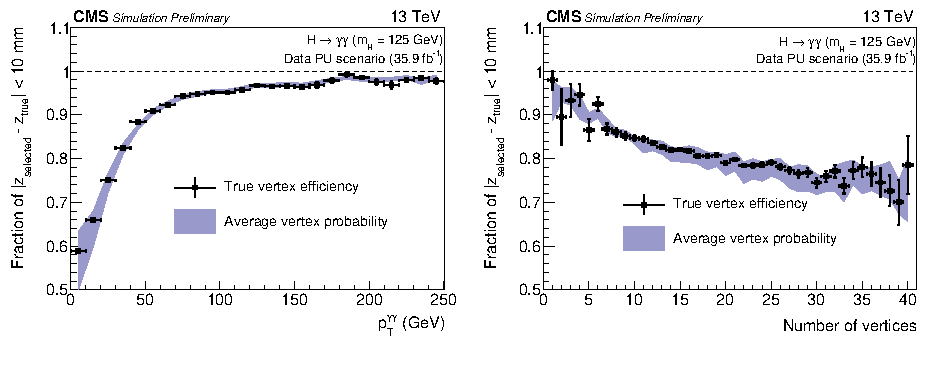
\includegraphics[width=0.95\textwidth]{figures/object_reco/CMS-PAS-HIG-16-040_Figure_004.pdf}
    \caption{Vertex ID efficiency as a function of diphoton $p_T$ (left) and number of event vertices (right).}
        \label{fig:object_reco:vertex_id_efficiency}
\end{figure}

Corrections are applied to account for discrepancies between data and simulation and a systematic uncertainty is assigned which is estimated by varying the ratio of data to simulation within their uncertainties. 

In simulated events the width of the distribution of beam spot longitudinal positions is a factor of $1.5$ wider than that measured in data. 
To compensate for this, simulated events with selected vertices more than $0.1$\,cm from the generator-level Higgs vertex are assigned a weighting that reproduces the width in data. 




\section{Photon Reconstruction}
Photons are reconstructed from calibrated ECAL superclusters which have had corrections calculated with a collection of techniques. One of these is a BDT regressor applied to account for detector effects. The resulting candidate photons are then put through a preselection aimed at rejecting non-prompt photons due to jet fragments, this also uses the output of a BDT classifier as a selection criterion.
All of these steps, including their validation, use a common collection of variables which will be detailed in the next subsection for later reference. 

\subsection{Common Variables}
The set of common variables can be divided into two main types: shower shape variables and isolation variables, plus some other miscellaneous variables. 
Shower shape variables describe properties of the electromagnetic showers within the ECAL which will allow us to infer information about the object. For example, whether a shower is from a pristine or a pair-converted photon.
The set of shower shape variables consists of the following:
\begin{itemize}[leftmargin=.5in,noitemsep]
    \item $E_{2\times{}2}/E_{5\times{}5}$: the ratio of energy in the $2\times{}2$ grid containing the most energetic crystal to the energy in the $5\times{}5$ grid around the SC seed crystal.
    \item $cov_{i\eta{i}\phi}$: the covariance of the crystal $\eta$ and $\phi$ locations within the $5\times{}5$ grid around the SC seed crystal. 
    \item $\sigma_{i\eta{}i\eta}$: pseudorapidity width of the shower in terms of crystals. 
    \item $R_{9}$: $E_{3\times{}3}/E_{SC}$, the ratio of the energy in the $3\times{}3$ grid around the SC seed crystal to the energy of the SC.
    \item $\sigma_{\eta}$: the logarithmic energy-weighted standard deviation of crystal $\eta$ in a SC.
    \item $\sigma_{\phi}$: the logarithmic energy-weighted standard deviation of crystal $\phi$ in a SC.
    \item $\sigma_{rr}$: the standard deviation of the shower width in the $x-y$ plane as measured by the preshower (only for photons measured in the endcaps).
\end{itemize}


Isolation variables measure how well-separated an object, in this case a photon, is from other objects in the event such as electrons or charged hadrons which could imitate the true signal. The set of isolation variables consists of the following
\begin{itemize}[leftmargin=.5in,noitemsep]
    \item $\mathcal{I}_{\gamma}$: photon isolation, the sum of the transverse energy of the particles identified as photons in a cone of $R=0.3$ around the candidate photon.
    \item $\mathcal{I}^{V}_{\mathrm{CH}}$: charged hadron isolation, the sum of transverse momenta of charged particles in a $R=0.3$ cone around the candidate photon associated with vertex $V$. 
    \item $\mathcal{I}_{\mathrm{T}}$: track isolation, the sum of transverse momenta of tracks in a hollow cone between $R=0.3$ and $R=0.04$ around the candidate photon.
    \item $H/E$: the ratio of energy measured in the HCAL to the energy measured in the ECAL in a cone of $R=0.15$ around the candidate photon.
\end{itemize}

Finally there are other miscellaneous variables used throughout the selection for different purposes,
\begin{itemize}[leftmargin=.5in,noitemsep]
    \item Electron veto: true or false if there is a track associated with the candidate SC.
    \item $\rho$: the event median energy density per unit area.
    \item $\eta_{SC}$: the pseudorapidity of the candidate SC.
    \item $E_{SC}^{RAW}$: the uncorrected energy of the candidate SC.
\end{itemize}



\subsection{Photon Energy Corrections}

The photon energy has a set of corrections applied depending on whether the photon is from simulation or data: individual photon energy correction, an overall energy scale correction in data, and a smearing of the simulated data to match its distribution to data. 

\subsubsection{Photon Energy Correction}
The photon energy correction is computed with a regressor BDT whose target is the ratio of true energy to the raw measured energy of the associated supercluster. It also computes the median uncertainty of the energy. 
The inputs to the BDT are a collection of shower shape variables, position variables, information from the preshower subdetector, and pileup-sensitive event-level variables.
The BDT is then trained on simulated photons with two separately trained BDTs in the barrel and endcap regions. 


\subsubsection{Energy Scale}
Once we have the corrected energies, the overall energy scale needs to be corrected to account for detector effects. 
During operation the CMS ECAL receives large doses of radiation that can degrade its performance over time. 
This will lead to drifts and jumps in the detector response as conditions change, and as a result the measured energy will also drift and jump. 
Scale factors to account for this effect in data are calculated using the $Z\rightarrow{}e^{+}e^{-}$ decay as a standard candle where the electrons are reconstructed as photons. 
Using comparison to simulation, and the well-known value of the $Z$ boson mass, scales are derived for different times and detector locations to bring the measured value of real $Z$ bosons back to the true value. 


\subsubsection{Resolution Smearing}
Simulation also needs to be corrected by comparison to data to make it more realistic. The photon energy resolution in simulated events has a Gaussian smearing added to it which is derived from comparing the width of the $Z\rightarrow{}e^{+}e^{-}$ mass distribution in different categories depending on $|\eta|$-location within the detector (two in the barrel either side of $|\eta|=1$ and two in the endcaps either side of $|\eta|=2$), and the $R_{9}$ variable which measures photon quality (above or below $R_{9}=0.94$).
The mass peak in two of these bins is shown in Figure \ref{fig:object_reco:invariant_mass_validation}.
\begin{figure}[h!]
    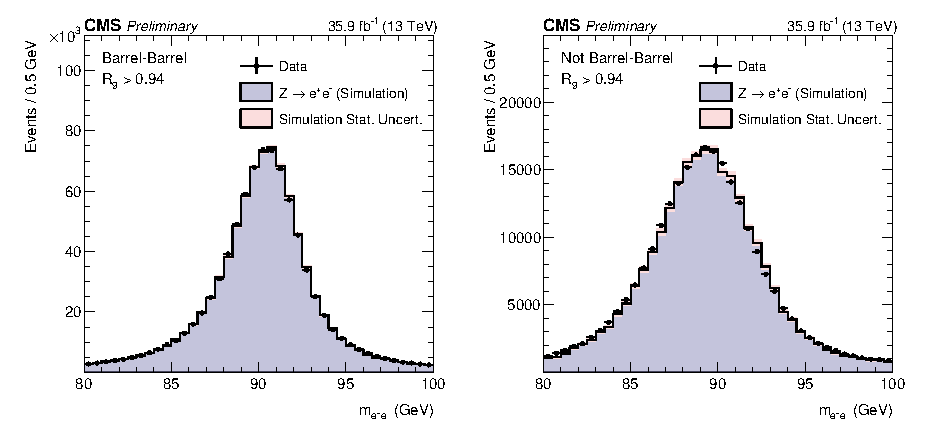
\includegraphics[width=0.95\textwidth]{figures/object_reco/CMS-PAS-HIG-16-040_Figure_001.pdf}
    \caption{A comparison between data and simulation of dielectron invariant mass}
        \label{fig:object_reco:invariant_mass_validation}
\end{figure}

\subsection{Photon Preselection}
%intro
Before a photon can enter the analysis it must pass a set of selection criteria, the photon preselection, which are slightly more stringent than the trigger and vary by location. First photons are grouped into candidate diphotons by considering all possible pairs in the event, then the criteria are applied (with the exception of $p_{T}$ cuts) on a per-photon basis.
The criteria are:
%List of requirements
\begin{itemize}[leftmargin=.5in,noitemsep]
    \item Electron veto: rejection if there is a track associated to the supercluster.
    \item Photon $p_{T}$s: $p_{T}^{\gamma_1} > 30$\,GeV and $p_{T}^{\gamma_2} > 20$\,GeV
    \item $R_{9}$: is not used to reject events outright, but determines which other selections are applied. If $R_{9} < 0.85$ in the barrel or $R_{9} < 0.9$ in the endcaps additional requirements are imposed. 
    \item Energy-weighted $\eta$ width: $\sigma_{\eta\eta} < 0.015$ in the barrel and $\sigma_{\eta\eta} < 0.015$ in the endcaps
    \item HCAL/ECAL deposition: $H/E < 0.08$ in all regions.
    \item Photon isolation: $\mathcal{I}_{\gamma} < 4.0$ in all regions. 
    \item Track isolation: $\mathcal{I}_{T} < 6.0$ in all regions.
    \item Charged hadron isolation: $\mathcal{I}_{CH} < 20$\,GeV.
    \item Photon ID: score from a BDT classifier that discriminates between prompt photons and jet fragments.
\end{itemize}
Both photons must also satisfy either of two additional requirements:
\begin{itemize}[leftmargin=.5in,noitemsep]
    \item $R_{9} > 0.8$ and $\mathcal{I}_{CH} < 20$\,GeV
    \item $\mathcal{I}_{CH}/p_{T}^{\gamma} < 0.3$
\end{itemize}

%Schema table of thesholds
The efficiency of these criteria are measured using $Z\rightarrow{}e^{+}e^{-}$ and the tag-and-probe method, 
with the exception of the electron veto which uses $Z\rightarrow{}\mu^{+}\mu^{-}\gamma$. The preselection efficiencies are summarised in Table \ref{tab:object_reco:presel_eff}
%Table of efficiencies
\begin{table}[h!]
    \begin{tabular}{ l | c | c | c }
        Preselection Category& $\epsilon_{\mathrm{data}} (\%)$ & $\epsilon_{\mathrm{sim}} (\%)$ & $\epsilon_{\mathrm{data}}/\epsilon_{\mathrm{sim}}$ \\
        \hline
        Barrel, $R_{9}>0.85$ & $94.2\pm0.9$ & $94.7\pm0.9$ & $0.995\pm0.001$ \\
        Barrel, $R_{9}<0.85$ & $82.5\pm0.7$ & $82.5\pm0.7$ & $1.000\pm0.003$ \\ 
        \hline
        Endcap, $R_{9}>0.85$ & $90.1\pm0.2$ & $91.3\pm0.1$ & $0.987\pm0.005$ \\ 
        Endcap, $R_{9}<0.85$ & $49.7\pm1.4$ & $53.8\pm1.5$ & $0.923\pm0.010$ \\ 
\end{tabular}
    \caption{Preselection efficiencies}
    \label{tab:object_reco:presel_eff}
\end{table}





\subsection{Photon Identification}
%Intro
The photon identification BDT is a classifier whose task is to discriminate between real prompt photons and photon-like jet fragments which satisfy the preselection criteria. 
The BDT is trained using simulated $\gamma + $jet events where the reconstructed photons are matched to a generator-level particle, if there is no match it is considered to be in the non-prompt class.
To avoid the BDT introducing a dependence on on photon kinematics the signal photons are re-weighted such that their distribution in $p_{T}$ and $\eta$ is flat. 
The classifier receives the following input features:
%variables
\begin{itemize}[leftmargin=.5in,noitemsep]
    \item Shower shape features: $\sigma_{i\eta{}i\eta}$, $cov_{i\eta{}i\phi}$, $E_{2\times{}2}/E_{5\times{}5}$, $R_{9}$, $\sigma_{\eta}$, $\sigma_{\phi}$, and $\sigma_{rr}$
    \item Isolation features: $\mathcal{I}_{\gamma}$, $\mathcal{I}_{CH}^{SV}$, and $\mathcal{I}_{CH}^{WV}$, where $SV$ and $WV$ refer to the selected vertex and worst vertex in terms of the vertex probability BDT respectively. 
    \item Other features: $\rho$, $\eta_{SC}$, $E_{SC}^{RAW}$, and $E_{ES}/E_{SC}^{RAW}$ where $E_{ES}$ is the energy measured by the ECAL preshower (endcaps only).
\end{itemize}

%validation 
The performance of this classifier is shown in Figure \ref{fig:object_reco:photon_id_bdt}. 
The systematic uncertainty on the BDT output is shown by the shaded region of the right hand plot. This is estimated so that it covers the largest disagreement between data and simulation of $Z\rightarrow{e^{+}e^{-}}$ reconstructed as photons in the endcap regions where agreement is worst.
\begin{figure}[h!]
    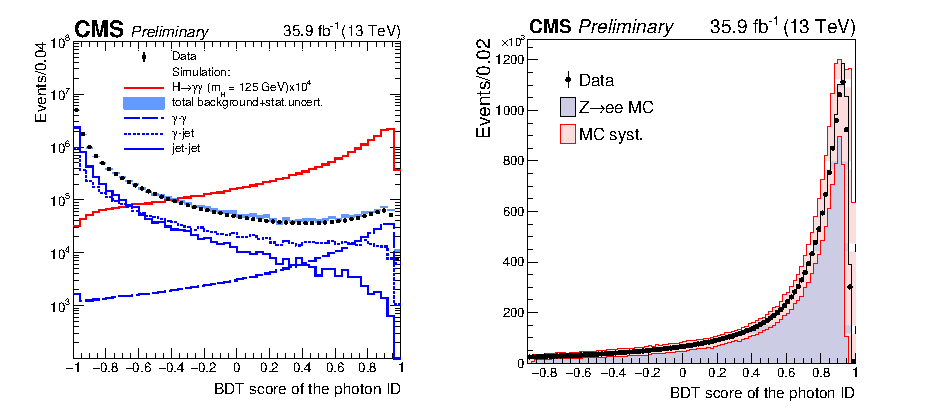
\includegraphics[width=0.95\textwidth]{figures/object_reco/CMS-PAS-HIG-16-040_Figure_002.pdf}
    \caption{Photon ID BDT performance and validation. (Left) Photon ID BDT output score of the lower-scoring photon of each diphoton passing the photon preselection. Signal photons from simulated Higgs events are shown in red and simulated background events are shown in blue, data is shown by the back dots. (Right) validation on $Z\rightarrow{e^{+}e^{-}}$ events.}
        \label{fig:object_reco:photon_id_bdt}
\end{figure}

A loose selection this BDT score is imposed as part of the photon preselection: $\hat{y} > -0.9$ where $\hat{y}$ is the output value. This selection keeps $99\%$ of the signal and removes a large portion of the background. This score is also used in later steps as a measure of photon quality: whether the photon is well-isolated and unconverted, or not. 


\section{Other Objects}

\subsection{Leptons}
Leptons are used for validation purposes throughout the analysis, and also event categorisation where there are leptons in the final state such as production with the ttH or VH modes. 
\subsubsection{Electrons}
Electrons are reconstructed in a similar way to photons, but with the extra requirement of an associated track. This association can be achieved in two ways depending on the properties of the candidate:
\begin{itemize}
    \item ECAL-based: starting with an energetic and well-isolated ECAL SC, match the track that is closest to the energy-weighted position of the SC and also within a window of $\Delta\eta=0.02$, $\Delta\phi=0.15$ of it.
    \item Tracker-based: starting with candidate tracks, associate them to a geometrically compatible SC. This is used for low $p_{T}$ electrons ($p_{T} < 10$\,GeV).
\end{itemize}
Candidates from both methods are combined to produce the set of PF candidate electrons of the event. 
There are also corrections applied to the tracks to correct for bremsstrahlung effects, and an energy correction from a BDT regressor analogous to the photon reconstruction. 

\subsubsection{Muons}
Hits in the muon system are formed into track segments and these are assembled via a clustering algorithm into muon system tracks called standalone muons. 
These are then associated with tracks from the inner tracker to produce global muons. A third approach is also used where inner tracks with $p_{T}<0.5$\,GeV and total $p < 2.5$\,GeV are extrapolated into the muon system. If a compatible muon segment is found this makes a `tracker muon'. Global muons and tracker muons that share the same inner track are merged into a single candidate. 
Standalone muons have worse momentum resolution and are more influenced by cosmic rays.

\subsection{Jets}
Jets are composite objects reconstructed from PF candidates using the anti-$k_T$ algorithm \cite{AntiKt} with $R=0.4$. 
The dedicated calibration for each PF candidate type, as well as 90\% of the jet energy being in the form of photons and charged hadrons allows for high-resolution measurement with the inner tracker and ECAL. The remaining 10\% consists of neutral hadrons which are measured at lower energy resolution in the HCAL \cite{JetPerformance}. 
The tracks also allow for the identification and rejection of particles originating from pileup vertices. Pileup gives extra energy to signal jets, and the soft pileup jets of these interactions can also be clustered into so-called fake jets of relatively large $p_{T}$ when they overlap. This latter effect rises quadratically with the number of pileup interactions. 

The jet objects receive corrections to their energy which relate the energy of the reconstructed jets to the energy at particle-level. A factorised approach is used \cite{JetPerformance}:
\begin{itemize}[leftmargin=.5in,noitemsep]
    \item First: subtracts $p_{T}^{offset}$ due to pileup influence. This is an average correction derived from the global per-event density $\rho$
    \item Second: corrects $p_{T}$ and $\eta$ dependence of the average jet detector response due to non-linearities in the calorimetry, differences in construction as a function of $\eta$, and $p_{T}$ thresholds.
    \item Jet energy scale: corrections for average residual discrepancies between data and simulation
\end{itemize}

In this analysis a collection of pileup mitigation techniques are employed. First, charged hadrons from vertices other than the chosen vertex are ignored within the tracker acceptance where this information is available. Outside the tracker a selection criterion is placed on the width of the jet expressed as
\begin{equation}
    \sigma_{RMS} = \frac{\sum_{i}p_{T}^{i^2}\Delta{R}^{i}}{\sum_{j}p_{T}^{j^2}}
\end{equation}
where $\Delta{R}^{i}$ is the distance between the constituent and the jet axis. The requirement is that $\sigma_{RMS} > 0.03$. 
Finally another technique uses a BDT classifier that takes a collection of jet shape variables and produces a score for each jet. A collection of selections on this score are then applied for bins in $p_{T}$ and $\eta$ (Table \ref{tab:object_reco:tight_pujid}).
Finally, in addition to the above, all jets are required to be within $|\eta| < 4.7$.

\begin{table}[h!]
    \begin{tabular}{ l || c | c | c | c }
         & $|\eta| < 2.5$ & $2.5 \leq |\eta| < 2.75$ & $2.75 \leq |\eta| < 3.0$ & $3.0 \leq |\eta| < 5.0$ \\
        \hline
        \hline
        $20 < p_{T} \leq 30$  & $0.69$ & $-0.35$ & $-0.26$ & $-0.21$ \\
        $30 < p_{T} \leq 50$  & $0.86$ & $-0.1$  & $-0.05$ & $-0.01$ \\
        $50 < p_{T} \leq 100$ & $0.95$ & $0.28$  & $0.31$  & $0.28$  \\
\end{tabular}
    \caption{Pileup jet ID cuts of the tight working point}
    \label{tab:object_reco:tight_pujid}
\end{table}







    \chapter{Event Categorisation}
\label{chap:event_select}

\newpage
\section{Overview and Objectives}
Once a set of candidate photons is assembled we tag and categorise events using extra final-state objects characteristic of particular Higgs production modes.
The objective of this tagging procedure is to enhance overall signficance, to construct categories of events with superior mass resolution, and to separate out the Higgs production modes for individual measurement. 


The event categorisation begins with a selection on the photon candidates with $p_{T}^{\gamma1}/m_{\gamma\gamma} > 1/3$, $p_{T}^{\gamma2}/m_{\gamma\gamma} > 1/4$, and $100 < m_{\gamma\gamma} < 180$\,GeV.
The use of mass-scaled $p_{T}$ here and in later machine learning models serves a dual purpose: firstly it avoids distortion of lower values in the $m_{\gamma\gamma}$ spectrum, secondly it avoids introducing mass bias from the simulated data during model trainings. 
There are then further requirements on the photons' supercluster pseudorapidities: both must have $|\eta| < 2.5$ to keep them in the fiducial region of the ECAL, and also must not be in the barrel-endcap transition region $1.44 < |\eta| < 1.57$ to ensure full containment of the electromagnetic showers. 


\subsection{The Diphoton BDT}
Selected diphoton candidates are then evaluated for signal-like kinematics and mass resolution by a BDT, the diphoton BDT, whose output score is used as a discriminating variable by the tags.
The input features of this BDT are the following:
\begin{itemize}[leftmargin=.5in,noitemsep]
    \item The mass-scaled transverse momentum $p^{\gamma}_{T}/m_{\gamma\gamma}$ for the leading and subleading photons
    \item The pseudorapidity $\eta$ for the leading and subleading photons
    \item The cosine of the azimuthal angle $\Delta\phi$ between the photons
    \item The score from the photon identification BDT for both photons
    \item The mass resolution estimate given the assumption that the correct vertex is selected, $\sigma^{RV}_{\gamma\gamma}/m_{\gamma\gamma}$
    \item The mass resolution estimate given the assumption that the incorrect vertex is selected, $\sigma^{WV}_{\gamma\gamma}/m_{\gamma\gamma}$
    \item The probability that the correct diphoton vertex has been selected, $p^{RV}$, estimated with the vertex probability BDT
\end{itemize}

%The in the right-vertex case, diphoton mass resolution is estimated by propagating the individual photon energy resolution estimates.

In the right vertex case the mass resolution is assumed to be completely dominated by the ECAL photon energy resolution. 
These can be approximated by Gaussian distributions and combined in quadrature to give the following expression for mass resolution,
\begin{equation}
    \sigma^{RV}_{\gamma\gamma} = \frac{1}{2}\sqrt{(\sigma^{E}_{\gamma{1}}/E_{\gamma{1}})^2 + (\sigma^{E}_{\gamma{2}}/E_{\gamma{2}})^2}
\end{equation} 
where $\sigma^{E}_{\gamma{1}}/E_{\gamma{1}}, \sigma^{E}_{\gamma{2}}/E_{\gamma{2}}$ are the relative uncertainties on the photon energies for the leading and subleading photons respectively. 

(Wrong vertex case)
In the wrong vertex case an extra contribution to the mass resolution from the vertex is summed in quadrature with the expression for the right vertex case. 
\begin{equation}
    \sigma^{WV}_{\gamma\gamma} = \frac{1}{2}\sqrt{(\sigma^{RV}_{\gamma\gamma}/m_{\gamma\gamma})^2 + (\sigma^{V}_{\gamma\gamma}/m_{\gamma\gamma})^2}
\end{equation} 
The assumption of a Gaussian-distributed uncertainty here is justified in the following way 
(see Louie's thesis)


(Training)
The diphoton BDT is trained on background and all signal samples with some funny weighting. 
Weighted according to their SM cross sections and expected mass resolution (?)
\begin{equation}
    w^{sig} = \frac{p^{RV}}{\sigma^{RV}_{\gamma\gamma}/m_{\gamma\gamma}} + \frac{1-p^{RV}}{\sigma^{WV}_{\gamma\gamma}/m_{\gamma\gamma}}
\end{equation} 
Weighting examples during training can be considered to be like setting a priority for their correct classification. 
This weighting will prioritise the correct classification of high mass resolution events, and production modes with a larger cross section. 

The diphoton BDT is validated with \Zee events reconstructed as diphotons. The perfomance of the diphoton BDT is shown in figure X


Figure \ref{fig:event_categorisaton:diphoton_bdt} shows the diphoton BDT score distributions for SM signal and background samples and for the \Zee control region
\begin{figure}[h!]
    \begin{center}
        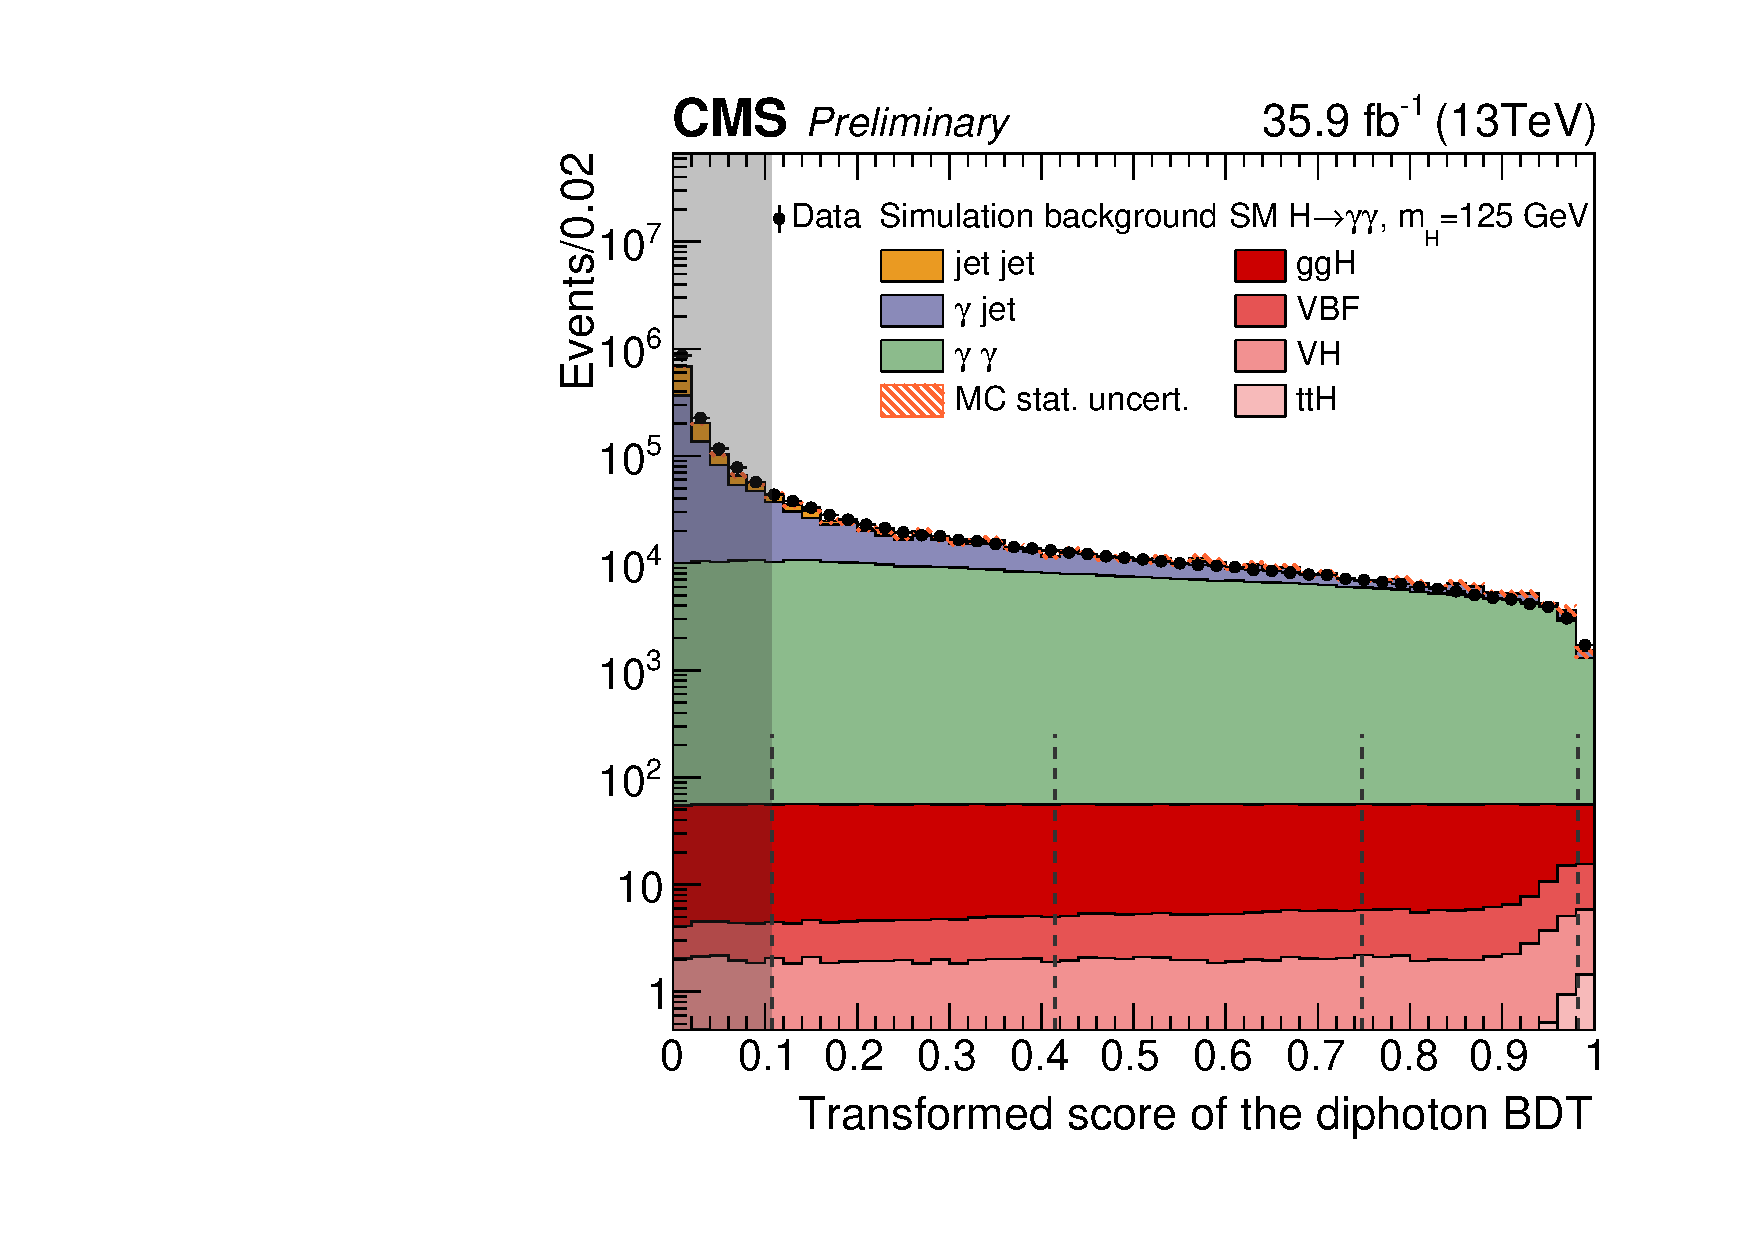
\includegraphics[width=0.49\textwidth]{figures/event_selection/Figure_005-a.pdf}
        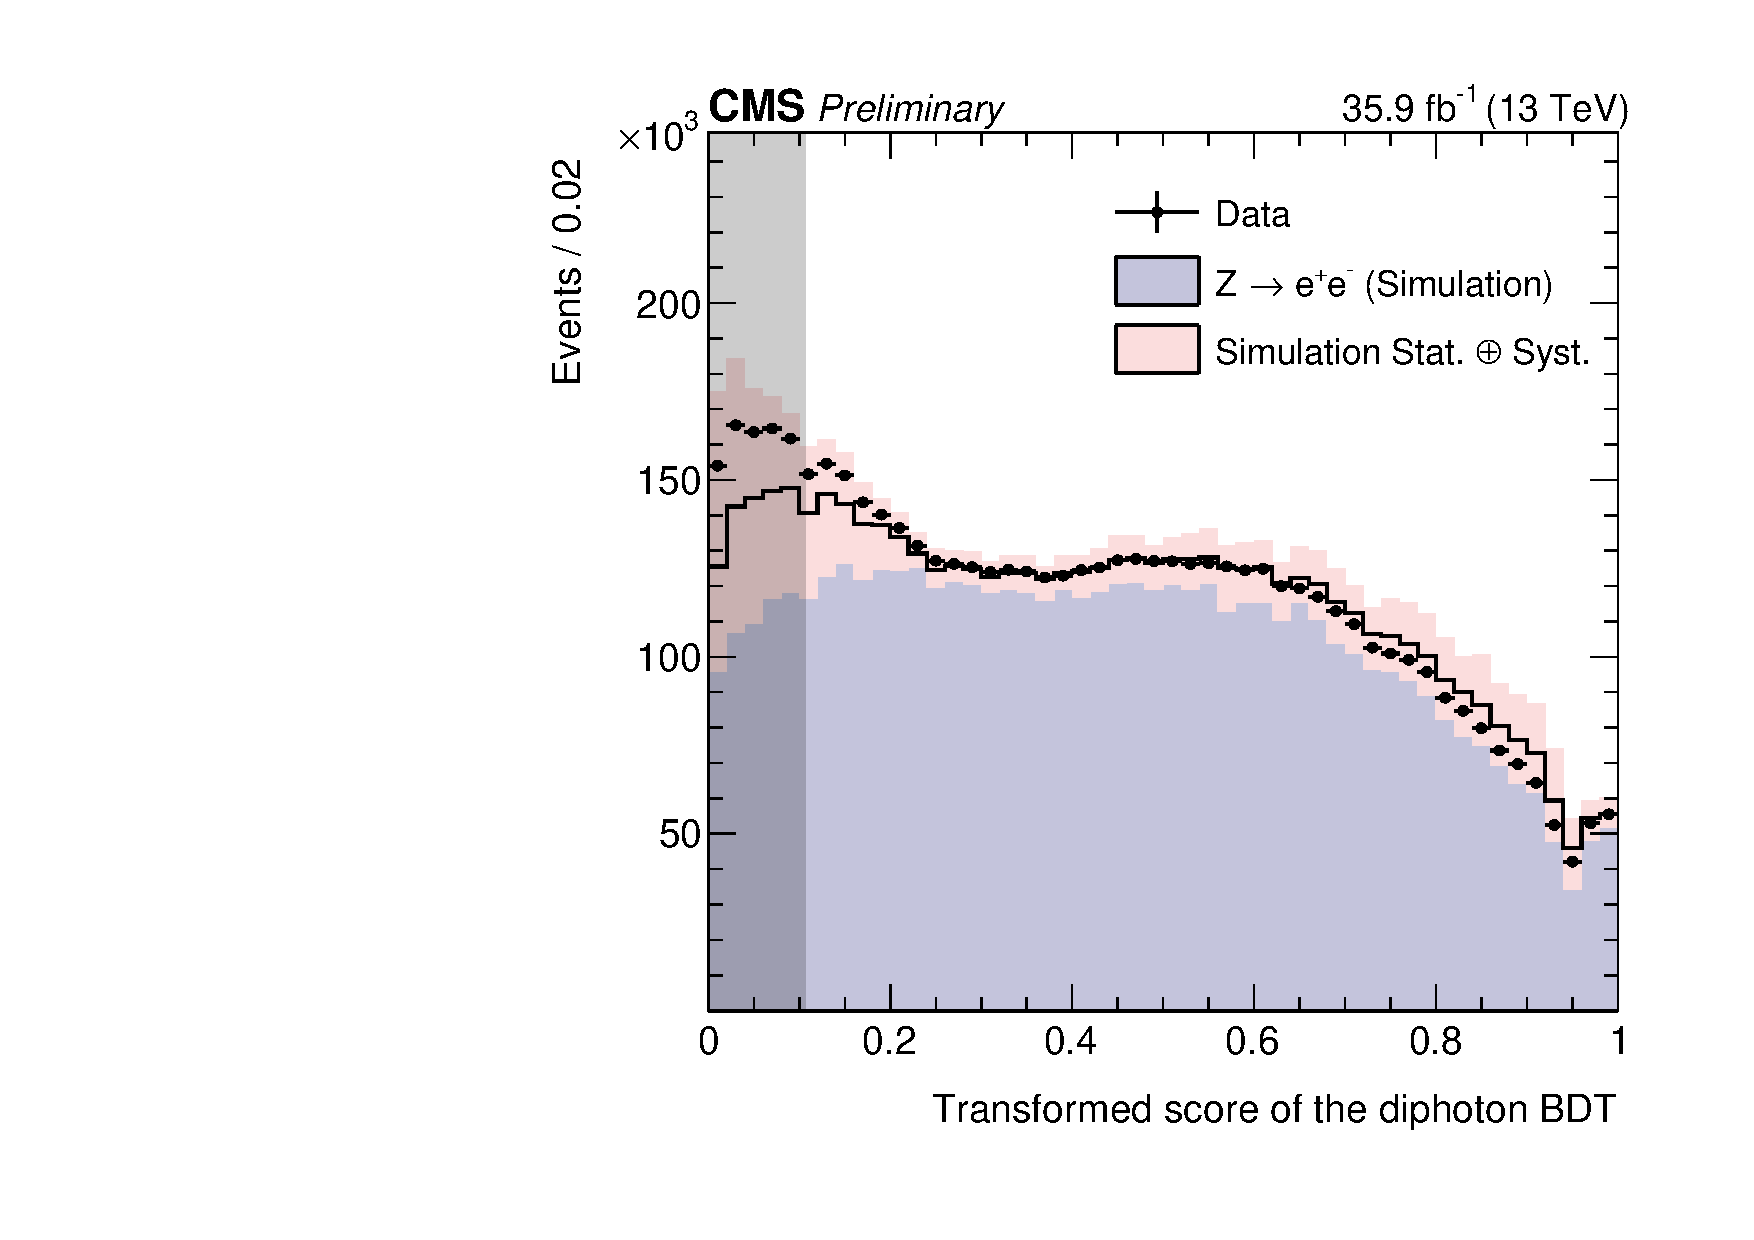
\includegraphics[width=0.49\textwidth]{figures/event_selection/Figure_005-b.pdf}
    \end{center}
    \caption{Crap figures with stupid flattened distributions}
        \label{fig:event_categorisaton:diphoton_bdt}
\end{figure}


\subsection{Tagging Scheme}
Tagging is implemented as a fall-through sequence where diphotons are offered to each tag in order of priority (Table \ref{tab:event_categorisaton:tag_sequence}). 
If a diphoton is not accepted by a tag it then passes to the next tag for consideration until the final `untagged' tag category. 
If the diphoton does not meet the criteria for this last tag it is discarded.
In the case of multiple tagged candidate diphotons in an event we select the one with the highest priority tag and category, if they are in the same category we choose the diphoton with the highest diphoton $p_{T}$.

\begin{table}[h!]
    \begin{tabular}{ l || l | l}
        Tag & Target Process & Structure \\
        \hline
        \ttH Leptonic      & \ttH with semi-leptonic top decays & Single category \\
        \ttH Hadronic      & \ttH with fully-hadronic top decays & Single category \\
        ZH Leptonic        & VH with leptonically-decaying Z boson & Single category \\
        WH Leptonic        & VH with leptonically-decaying W boson & Single category \\
        VH Leptonic Loose  & VH with leptonically-decaying W or Z boson & Single category \\
        VBF                & VBF with dijet in the final state & Three categories \\
        VH MET            & VH with significant amount of \MET & Single category \\
        VH Hadronic        & VH with hadronically-decaying W or Z boson & Single category \\
        Untagged           & Inclusive & Four categories \\
    \end{tabular}
    \caption{The \Hgg tag sequence}
    \label{tab:event_categorisaton:tag_sequence}
\end{table}

In the remainder of this chapter we will describe each tag grouped by the production mode they target. In particular we will consider VBF tagging in detail and present a tag based on jet images and a dense CNN. 






\section{Top Fusion Tagging}
In the \ttH production mode, a top-antitop pair is produced in association with the Higgs boson. The top quark immediately decays to a b quark and a W boson which will subsequently decay leptonically or hadronically. In the former (semi-leptonic) case there will be a bottom quark jet plus an associated lepton with \MET from the W decay. In the latter (fully-hadronic) case there will be a bottom quark jet plus two quark jets from the W decay to quarks (Figure \ref{fig:event_categorisaton:top_decays}). 

\begin{figure}[h!]
    \begin{center}
        \begin{tikzpicture}[baseline=(current bounding box.center)]
        \begin{feynman}
            \vertex (a) {$t$};
            \vertex [right=of a] (b);
            \vertex [above right=of b] (f1);
            \vertex [below right=of b] (f2) {$b$};
            \vertex [above right=of f1] (f3) {$q_{(u,c,t)}$};
            \vertex [below right=of f1] (f4) {$\bar{q}_{(d,s,b)}$};
            \diagram* {
                (a) -- [fermion] (b) -- [boson, edge label=\(W^{+}\)] (f1),
                (b) -- [fermion] (f2),
                (f1) -- [fermion] (f3),
                (f4) -- [fermion] (f1),
            };
        \end{feynman}
        \end{tikzpicture}
        %
        \qquad
        \begin{tikzpicture}[baseline=(current bounding box.center)]
        \begin{feynman}
            \vertex (a) {$t$};
            \vertex [right=of a] (b);
            \vertex [above right=of b] (f1);
            \vertex [below right=of b] (f2) {$b$};
            \vertex [above right=of f1] (f3) {$\bar{\ell}$};
            \vertex [below right=of f1] (f4) {${\nu_{\ell}}$};
            \diagram* {
                (a) -- [fermion] (b) -- [boson, edge label=\(W^{+}\)] (f1),
                (b) -- [fermion] (f2),
                (f1) -- [fermion] (f3),
                (f4) -- [fermion] (f1),
            };
        \end{feynman}
        \end{tikzpicture}
    \end{center}
    \caption{Top quark decay modes: a fully-hadronic decay (left) and a semi-leptonic decay (right).}
    \label{fig:event_categorisaton:top_decays}
\end{figure}

The top tags target these two decay modes: the leptonic tag searches for \ttH events where at least one top quark decays semi-leptonically, and the hadronic tag searches for \ttH events where both top quarks decay fully-hadronically. 

\subsection{\ttH Leptonic}
This tag uses a set of selections on kinematic properties of leptons and jets in the event. 
Leptons are required to pass selection requirements depending on their flavour
\begin{itemize}[leftmargin=.5in,noitemsep]
    \item Diphoton BDT score $> 0.11$ 
    \item At least one selected lepton with $p_{T} > 20$\,GeV
    \item All selected leptons are required to have an angular separation from a signal photon of $R(\ell,\gamma) > 0.35$
    \item $|m_{e\gamma} - m_{Z}| > 5$\,GeV (electrons only)
    \item A minimum of two jets in the event with $p_{T} > 25$\,GeV, $|\eta| < 2.4$, $R(j,\gamma) > 0.4$ and $R(j,\ell) > 0.4$
    \item At least one jet is tagged as b jet by the CSV tagger (medium requirement)
\end{itemize}


\subsection{\ttH Hadronic}
This tag uses a set of selections on kinematic properties of the jets in the event, as well as a dedicated BDT. The \ttH hadronic BDT is trained on the following input features:
\begin{itemize}[leftmargin=.5in,noitemsep]
    \item the number of jets with $p_{T} > 25$\,GeV,
    \item the $p_{T}$ of the leading jet,
    \item the two highest scores of the CSV b-tagger.
\end{itemize}
A selection on the BDT output score (Figure \ref{fig:event_categorisaton:tth_hadronic_bdt}) is optimised simultaneously on simulation with a selection on the diphoton BDT score to maximise expected precision on the signal strength of the \ttH production channel. 

\begin{figure}[h!]
    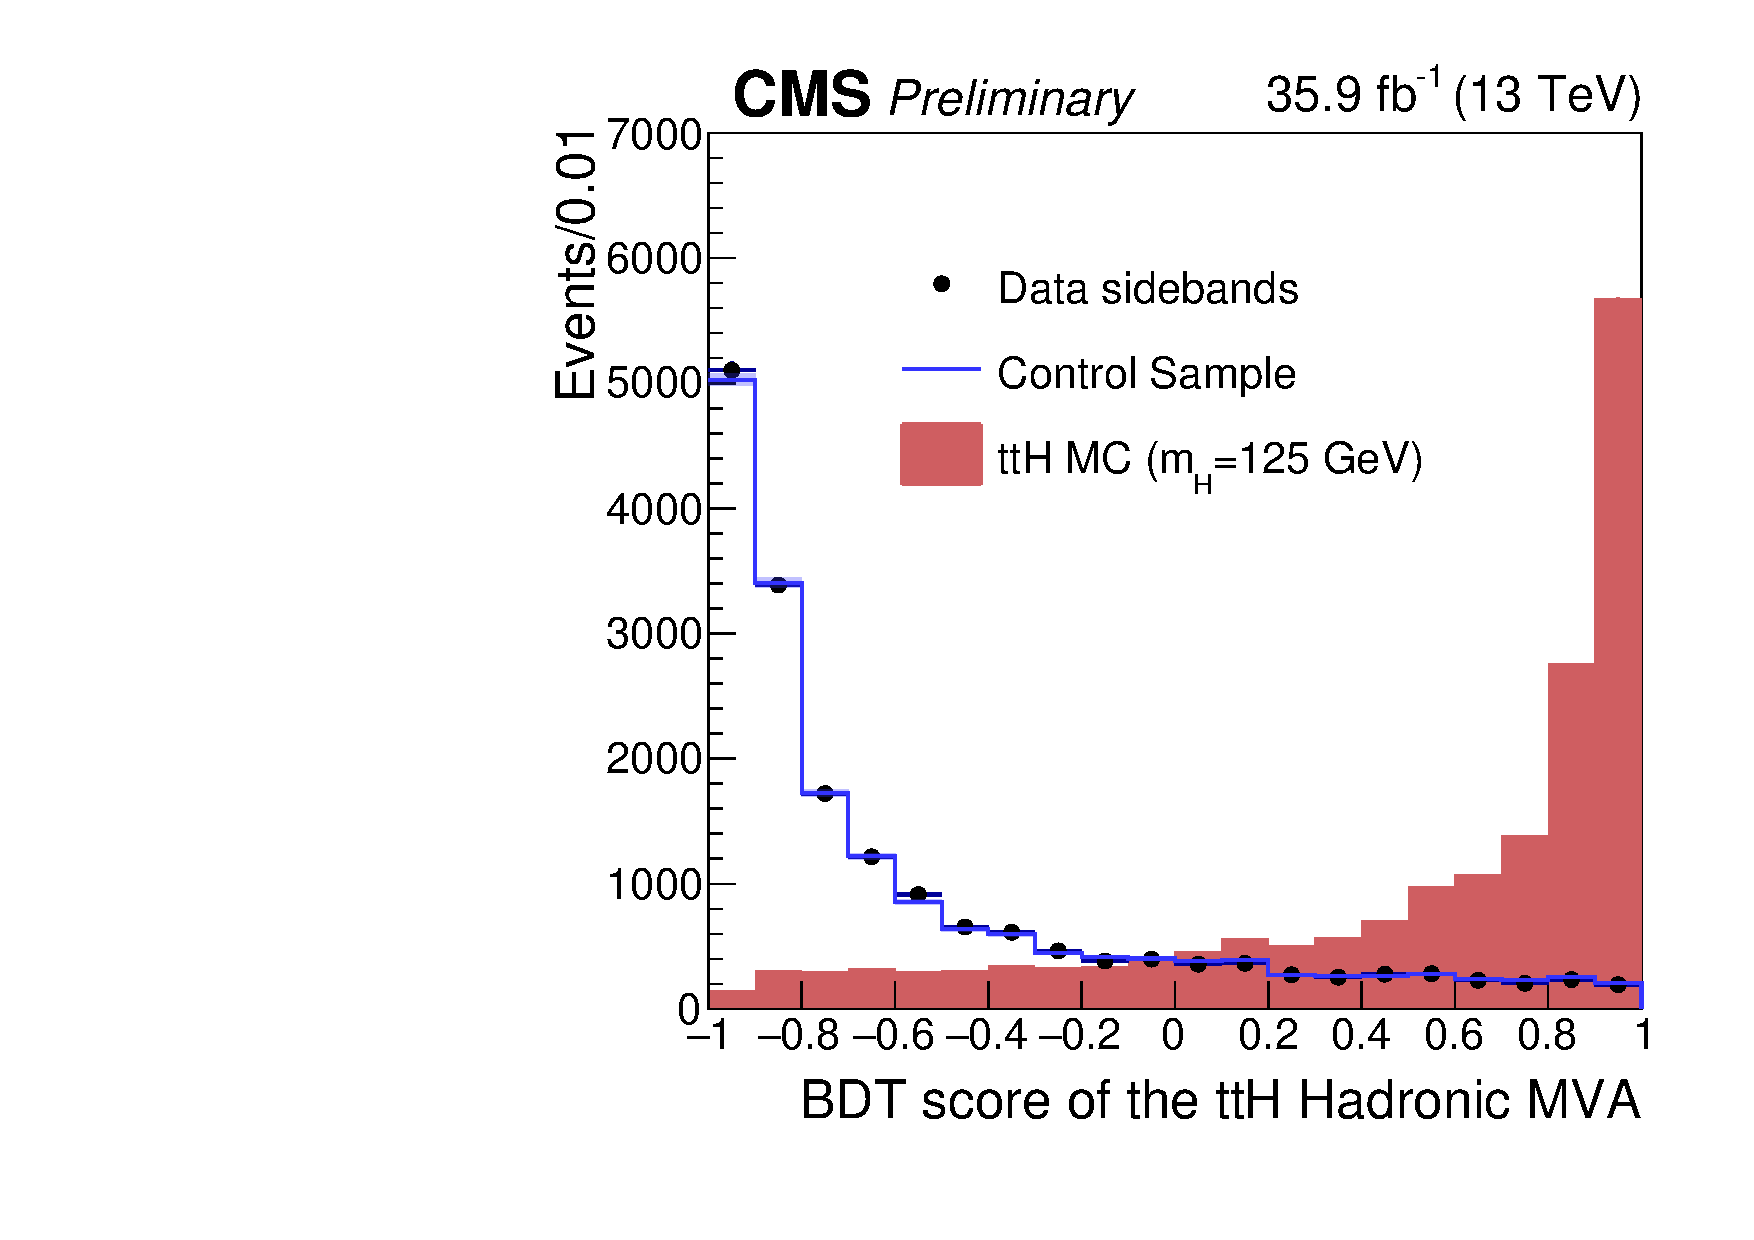
\includegraphics[width=0.49\textwidth]{figures/event_selection/Figure_006.pdf}
    \caption{Score distribution of the hadronic \ttH BDT. The blue lined histogram shows the distribution for the control region, the red filled histogram shows the score distribution for simulated signal, and the points show the score distribution of the data sideband regions ($m_{\gamma\gamma} < 115$\,GeV or $m_{\gamma\gamma} > 135$\,GeV).}
        \label{fig:event_categorisaton:tth_hadronic_bdt}
\end{figure}

A control region is constructed by selecting photon pairs where one passes the preselection and photon ID requirements, whilst the other has no preselection requirement and the photon ID is inverted.
These events are then weighted in $\eta$ and $p_T$ of the photons to reproduce the kinematic properties of the signal region.

The selection requirements of the \ttH Hadronic tag are as follows:
\begin{itemize}[leftmargin=.5in,noitemsep]
    \item $p_{T}/m_{\gamma\gamma} > 1/3$ and $1/4$ for leading and subleading photons respectively,
    \item diphoton BDT score $> 0.4$,
    \item no leptons that meet the criteria of the \ttH Leptonic tag
    \item a minimum of three jets in the event with $p_{T} > 25$\,GeV and $|\eta| < 2.4$,
    \item at least one jet is tagged as b jet by the CSV tagger (medium requirement),
    \item a \ttH Hadronic BDT score above 0.75.
\end{itemize}



\section{Associated Production Tagging}
In the associated production (VH) mode a W or Z is produced in association with the Higgs boson. The VH tags target different vector bosons decaying in different ways which can manifest as leptons, jets or \MET in the event.
All of the leptonic VH tags are selection-based and have various isolation requirements to avoid contamination from Drell-Yan background processes.

\subsection{ZH Leptonic}
Targets Higgs production in association with a Z boson that subsequently decays leptonically with stringent requirements. The selection criteria are as follows:
\begin{itemize}[leftmargin=.5in,noitemsep]
    \item $p_{T}/m_{\gamma\gamma} > 3/8$ and $1/4$ for leading and subleading photons respectively,
    \item diphoton BDT score $> 0.11$,
    \item two same-flavour leptons with $p_T > 20$\,GeV and satisfying the same requirements as in the \ttH Leptonic tag
    \item $70 < m_{\ell\ell} < 110$\,GeV,
    \item $R(\gamma,e) > 1.0$, or $R(\gamma,\mu) > 0.5$,
    \item conversion electron veto: if an electron and a photon share a supercluser, the electron track must be well-separated from the supercluser centre ($R(SC,e_{\mathrm{track}}) > 0.4$).
\end{itemize}


\subsection{WH Leptonic}
Targets Higgs production in association with a W$^{\pm}$ boson that subsequently decays leptonically with stringent requirements. The selection criteria are as follows:
\begin{itemize}[leftmargin=.5in,noitemsep]
    \item $p_{T}/m_{\gamma\gamma} > 3/8$ and $1/4$ for leading and subleading photons respectively,
    \item diphoton BDT score $> 0.28$,
    \item at minimum one lepton with $p_T > 20$\,GeV and satisfying the same requirements as in the \ttH Leptonic tag
    \item $R(\gamma,\ell) > 1.0$,
    \item \MET$> 45$\,GeV,
    \item a maximum of two jets each satisfying $p_T > 20$\,GeV, $|\eta| < 2.4$, $R(j,\ell) > 0.4$, $R(j,\gamma) > 0.4$,
    \item electron conversion veto as in the ZH Leptonic tag
\end{itemize}



\subsection{VH Leptonic Loose}
Targets Higgs production in association with either W$^{\pm}$ or Z which then decay leptonically. This tag uses a looser \MET selection of \MET$ < 45$\, GeV, with the rest of the selection being the same as WH Leptonic.

\subsection{VH MET}
Targets Higgs associated production with \MET from at least one missing lepton. The selection criteria are as follows:
\begin{itemize}[leftmargin=.5in,noitemsep]
    \item $p_{T}/m_{\gamma\gamma} > 3/8$ and $1/4$ for leading and subleading photons respectively,
    \item diphoton BDT score $> 0.79$,
    \item \MET$> 85$\,GeV,
    \item $|\Delta\phi(\gamma\gamma,E_{T}^{miss})| > 2.4$
\end{itemize}


\subsection{VH Hadronic}
Targets Higgs production in association with a W or Z boson that decays hadronically. The selection criteria are as follows:
\begin{itemize}[leftmargin=.5in,noitemsep]
    \item $p_{T}/m_{\gamma\gamma} > 1/2$ and $1/4$ for leading and subleading photons respectively, 
    \item diphoton BDT score $> 0.79$,
    \item a minimum of two jets with $p_T > 40$\,GeV and $|\eta| < 2.4$, $R(j,\gamma) > 0.4$,
    \item dijet invariant mass $60 < m_{jj} < 120$\,GeV,
    \item $|\mathrm{cos}{\theta^{*}}|$
\end{itemize}









\section{VBF Tag: Legacy}
The VBF production mode is characterised by its distinctive event topology and kinematics: two high-$p_{T}$ jets with large pseudorapidity separation. Furthermore, the dijet substructure will also be distinctive with both jets originating from quarks and having colour connection to the proton remnant. 

Other production modes can also produce a Higgs boson in association with jets. In particular, ggH can be a significant source of false positives due to its larger cross section and capacity to produce jets in next-to-leading order processes and from initial-state radiation at leading order. 

VBF tagging targets the VBF production mode by exploiting the distinctive properties of VBF dijets. In this section we will explore two approaches:
\begin{itemize}[leftmargin=.5in,noitemsep]
    \item A tag based on two BDTs with engineered kinematic features. This is the approach used in the 2016 \Hgg analysis. 
    \item A tag based on a single dense convolutional neural network that receives jet structure information in the form of images in addition to engineered kinematic features. 
\end{itemize}
Both tags use the same event preselection, and produce scores used to define event categories which enhance the expected significance of the VBF channel. 
The measure of significance used here is the approximate mean significance (AMS) which was introduced in the Higgs ML challenge (ref),
\begin{equation}
    \mathrm{AMS}_{2} = \sqrt{2\left( (s+b+b_{\mathrm{reg}})\log\left(1 + \frac{s}{b+b_{\mathrm{reg}}}\right) - s \right)}.
\end{equation}
Where $s$ is the total number of signal events, $b$ is the total number of background events, and $b_{\mathrm{reg}}$ is a regularisation term that reduces sensitivity to local optima due to spiky distributions. 

The legacy tag consists of two BDTs chained together which integrate different information to form a discriminant score. 
The first of these, the djiet BDT, evaluates how signal-like the events are based on kinematic information from the dijet and its relationship with the diphoton. 
The second BDT, the combined BDT, integrates information from multiple sources to produce the final discriminant score for classification. 

\subsection{Selection}

\subsubsection{Jet Selection}
Selection criteria are applied to individiual jets in addition to those described in the previous chapter before being considered for making the dijet. 
(The selections on the individual jets)
(PUJID because AMS value, mention Zee $\eta$ agreement stuff)




\subsubsection{Dijet Selection}
Dijets are formed by selecting the two highest-$p_T$ jets in the event which pass the jet selection requirements. If there are fewer than two jets the event is rejected by the VBF tag and falls through to untagged. 
Candidate dijets are required to meet the following selection:
\begin{itemize}[leftmargin=.5in,noitemsep]
    \item $p_{T}/m_{\gamma\gamma} > 1/3$ and $1/4$ for leading and subleading photon respectively,
    \item photon ID BDT score $> -0.2$ for both photons,
    \item dijet invariant mass $m_{jj} > 250$\,GeV,
    \item jet $p_{T} > 40$\,GeV and $> 30$\,GeV for the leading and subleading jets respectively,
    \item absolute pseudorapidity $|\eta| < 4.7$ for both jets.
\end{itemize}

The photon ID score requirement is due to the diphoton BDT assigning a high score to background diphotons which have a low photon ID score.
This is occuring becuase the diphoton BDT is trained over multiple signal processes with a cross-section weighting, this in turn leads to it to prioritise the accurate classification of ggH-like events where a diphoton is produced without associated objects. 
Signal events in the VBF phase space have a lower weighting and therefore the diphoton BDT does not separate these with the same level of priority. 
A strong indicator of ggH signal is that the diphoton has high $p_T$. The BDT appears to be allowing high-$p_T$ background events through without applying photon ID requirements. The photon ID cut of the VBF tag is aimed at reducing this effect. 







\subsection{Dijet BDT}
BDT that targets signal-like dijet kinematics. Receives the following features which are unbiased with respect to mass by construction:
\begin{itemize}[leftmargin=.5in,noitemsep]
    \item $p_{T}/m_{\gamma\gamma}$ for the leading and subleading photons
    \item $p_{T}^{j1}$ and $p_{T}^{j2}$, the transverse momenta of the leading and subleading jets respectively
    \item $m_{jj}$ the invariant mass of the dijet
    \item $\Delta\eta$ the pseudorapidity gap between the two jets
    \item $\mathrm{min}\Delta{R}(\gamma,j)$ the smallest angular separation between either of the diphoton photons and either of the dijet jets
    \item $|\Delta\phi_{\gamma\gamma{jj}}|$ the absolute azimuthal angular difference between the diphoton and dijet
    \item $|\Delta\phi_{jj}|$ the absolute azimuthal angular difference between the jets of the dijet
    \item $C_{\gamma\gamma}$ the diphoton centrality expressed as:
        \begin{equation}
            C_{\gamma\gamma} = \mathrm{exp}\left(-\frac{4}{(\eta_{j1} - \eta_{j2})^{2}}\left( \eta_{\gamma\gamma} - \frac{\eta_{j1} + \eta_{j2}}{2} \right)^{2}\right)
        \end{equation}
\end{itemize}




\begin{figure}[h!]
    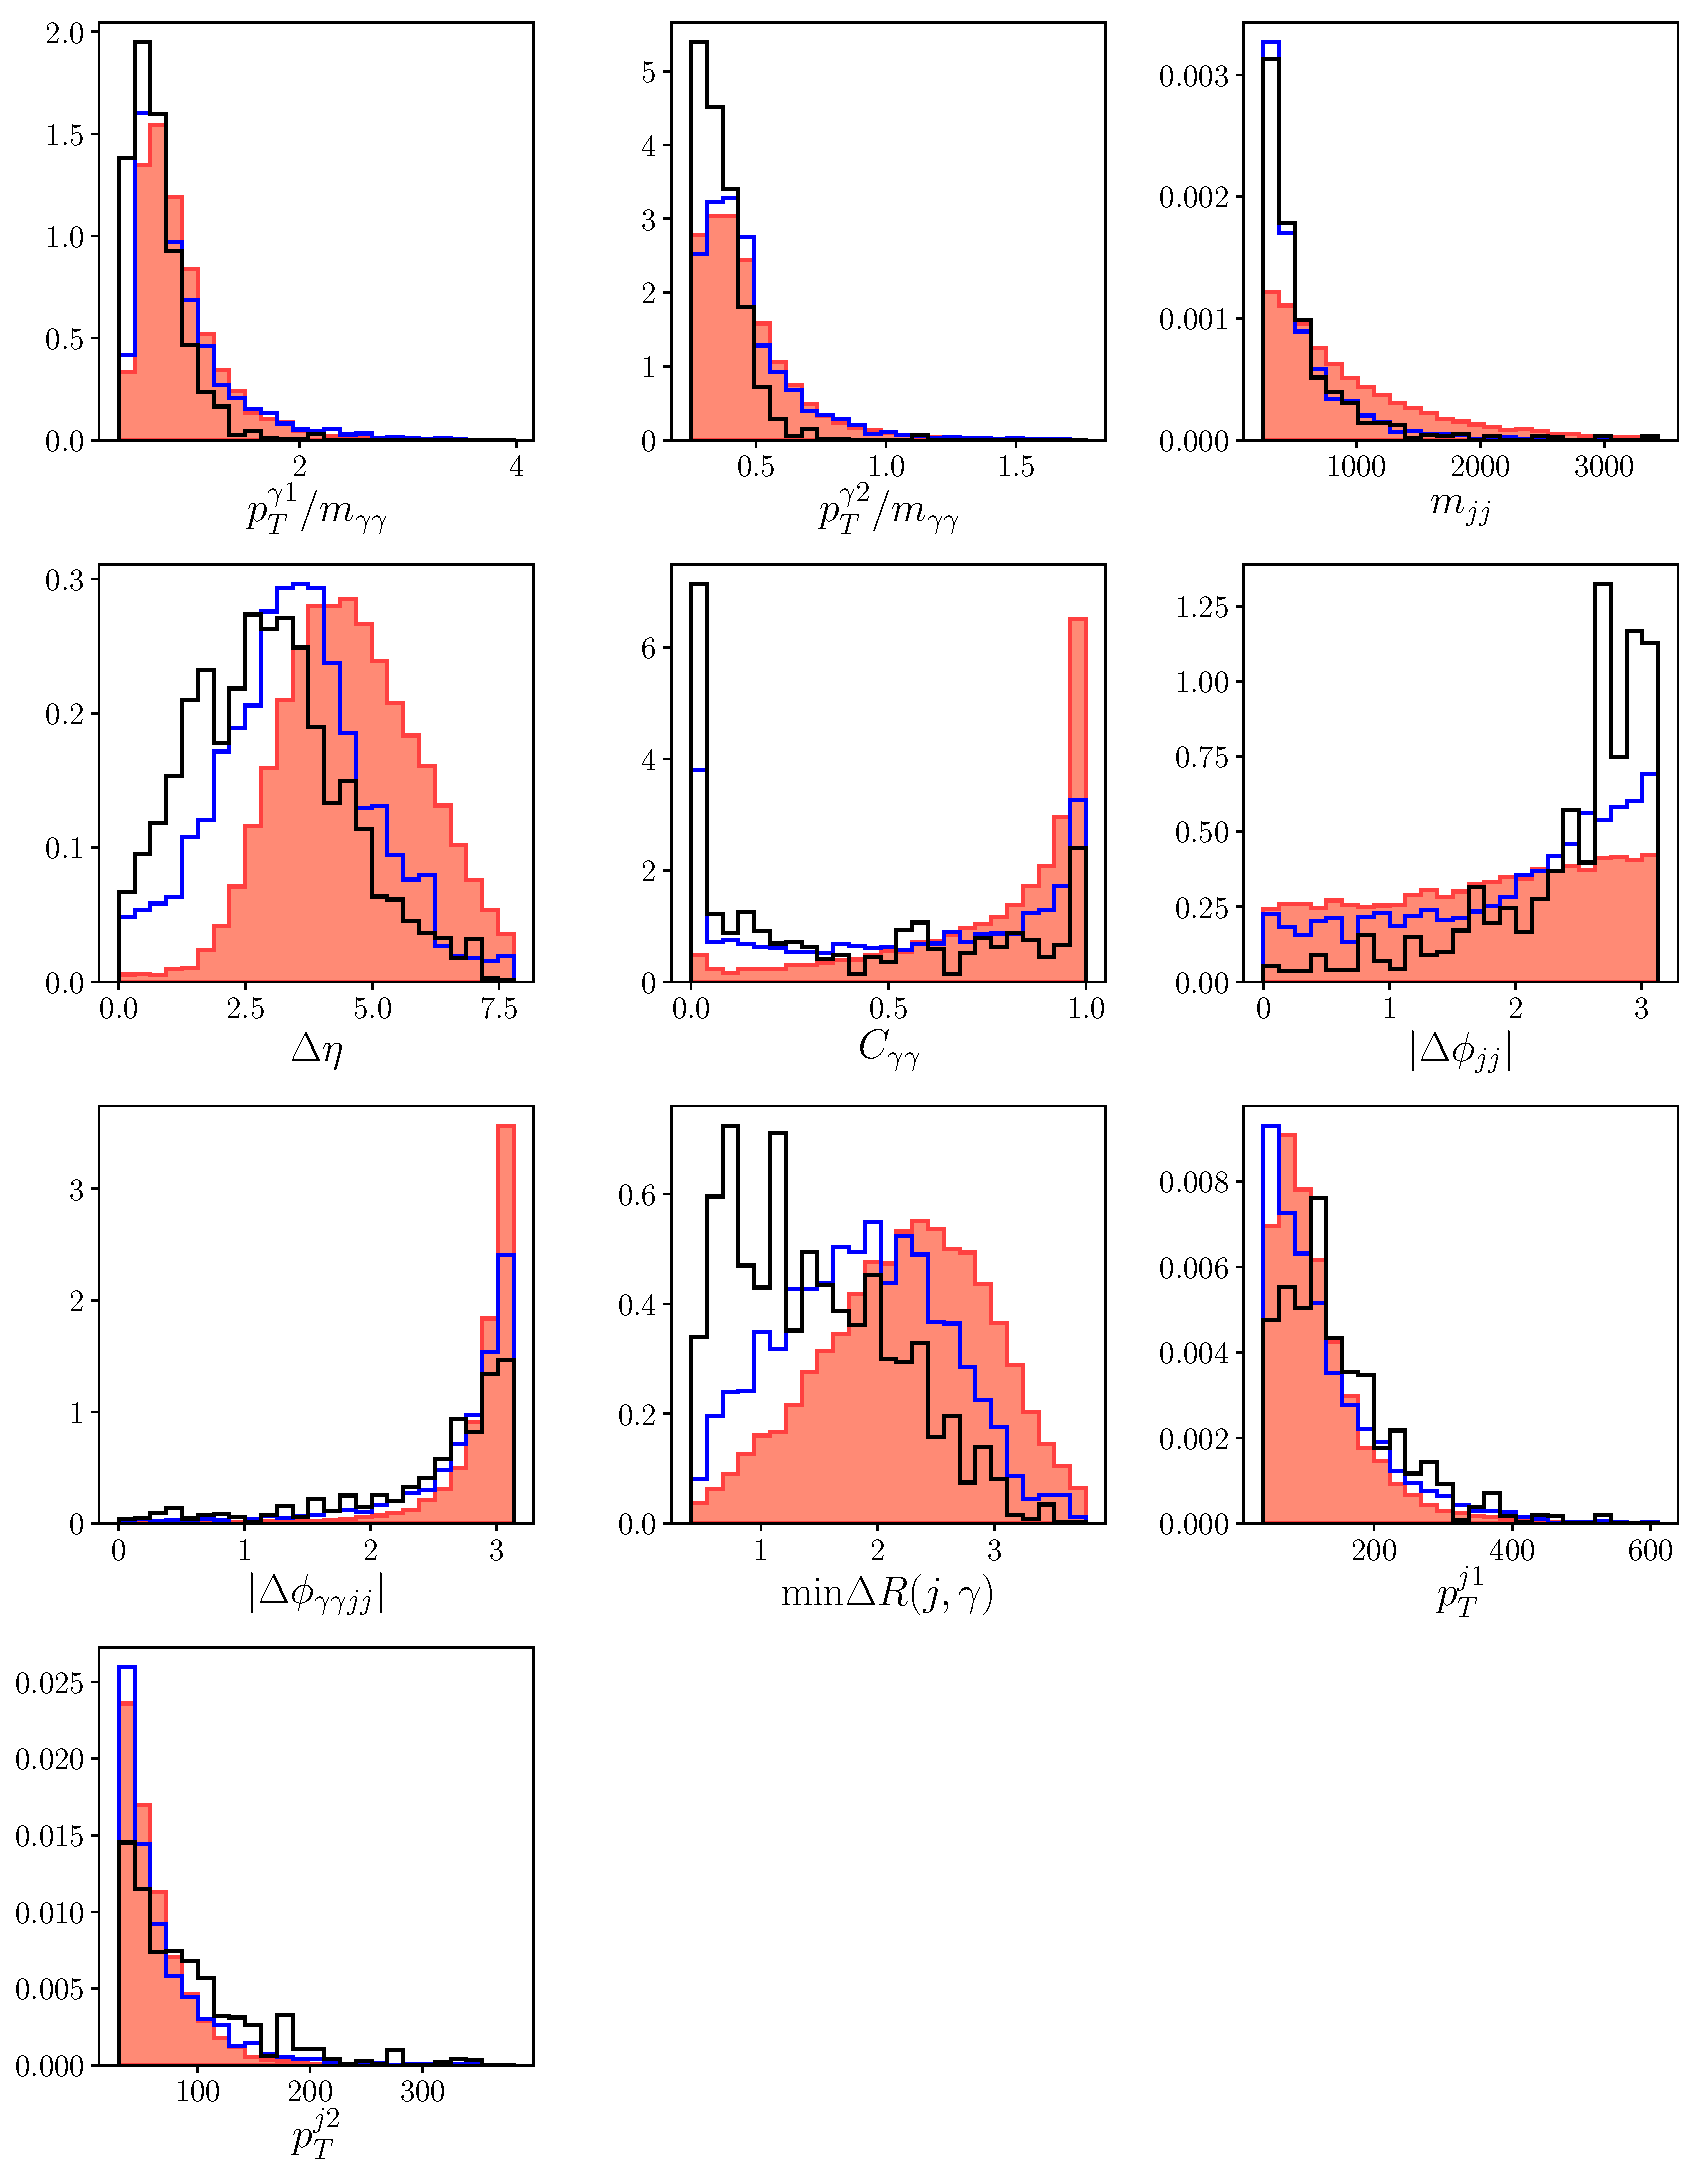
\includegraphics[width=0.90\textwidth]{figures/event_selection/dijet_BDT_features_PS.pdf}
    \caption{Dijet BDT feature distributions with the full VBF preselection. Distributions are all normalised to unity with solid red corresponding to VBF, blue line to ggH, and black line to SM background}
    \label{fig:event_categorisaton:dijet_bdt_features}
\end{figure}


\subsection{Combined BDT}
BDT that takes all the information and gives the final score
\begin{itemize}[leftmargin=.5in,noitemsep]
    \item diphoton BDT score
    \item dijet BDT score
    \item $p_{T}^{\gamma\gamma}/m_{\gamma\gamma}$, the mass-scaled transverse momentum of the diphoton
\end{itemize}

\begin{figure}[h!]
    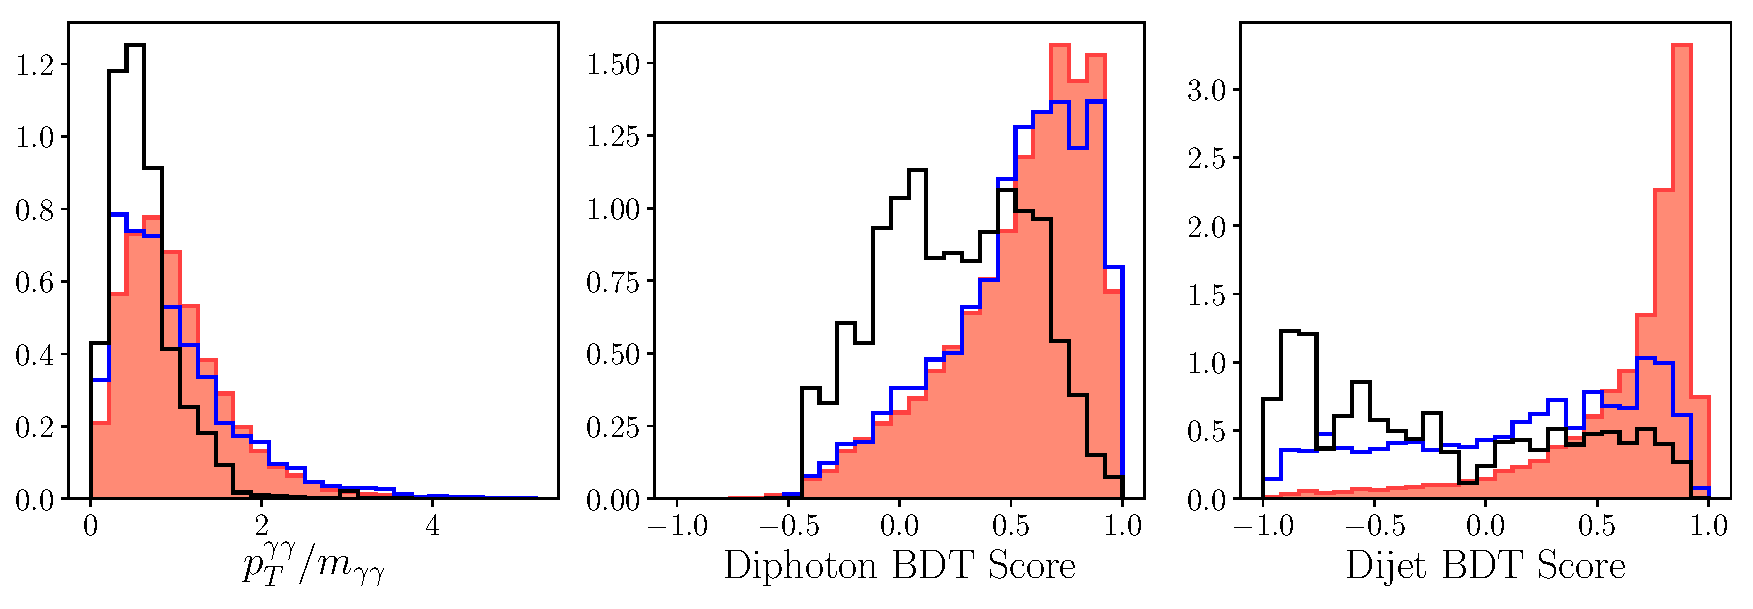
\includegraphics[width=0.90\textwidth]{figures/event_selection/combined_BDT_features_PS.pdf}
    \caption{Combined BDT feature distributions with the full VBF preselection. Distributions are all normalised to unity with solid red corresponding to VBF, blue line to ggH, and black line to SM background}
    \label{fig:event_categorisaton:combined_bdt_features}
\end{figure}

\begin{figure}[h!]
    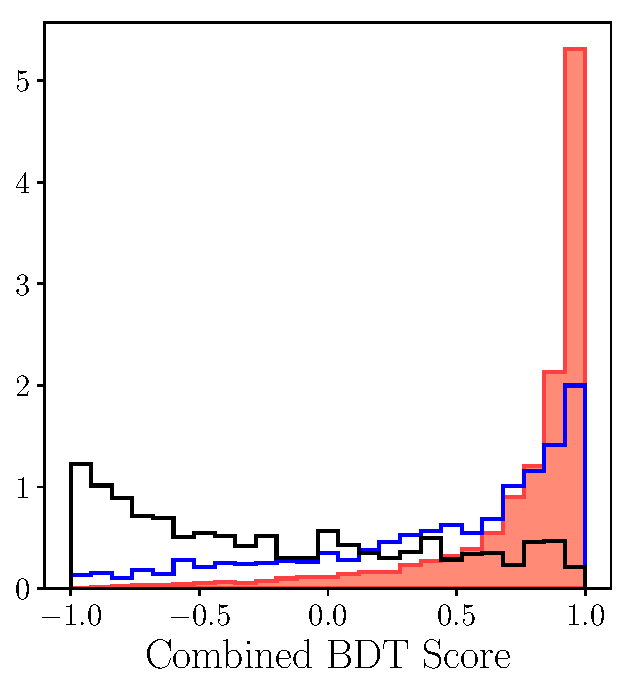
\includegraphics[width=0.4\textwidth]{figures/event_selection/combined_BDT_score.pdf}
    \caption{Combined BDT score distribution with the full VBF preselection. Distributions are all normalised to unity with solid red corresponding to VBF, blue line to ggH, and black line to SM background}
    \label{fig:event_categorisaton:combined_bdt_features}
\end{figure}





\subsection{Categorisation}
Boundary opt for overall significance


\subsection{Validation}
We define a control region in \Zee events where the electron veto has been inverted and the electrons reconstructed as photons. In addition to the electrons we require two jets with the following selection which mimics the phase space of the VBF tag:

\begin{itemize}[leftmargin=.5in,noitemsep]
    \item $p_{T}^{j1} > 40$, and $p_{T}^{j1} > 30$ for the leading and subleading jets,
    \item $p_{T}^{\gamma{1}} > 1/3$ and $p_{T}^{\gamma{2}} > 1/4$ for the leading and subleading photons.
\end{itemize}
There is no requirement on the dijet mass $m_{jj}$. 

The control region is used for simulation/data comparison of both the features input to the BDTs and the output scores. 

\begin{figure}[h!]
    \begin{center}
        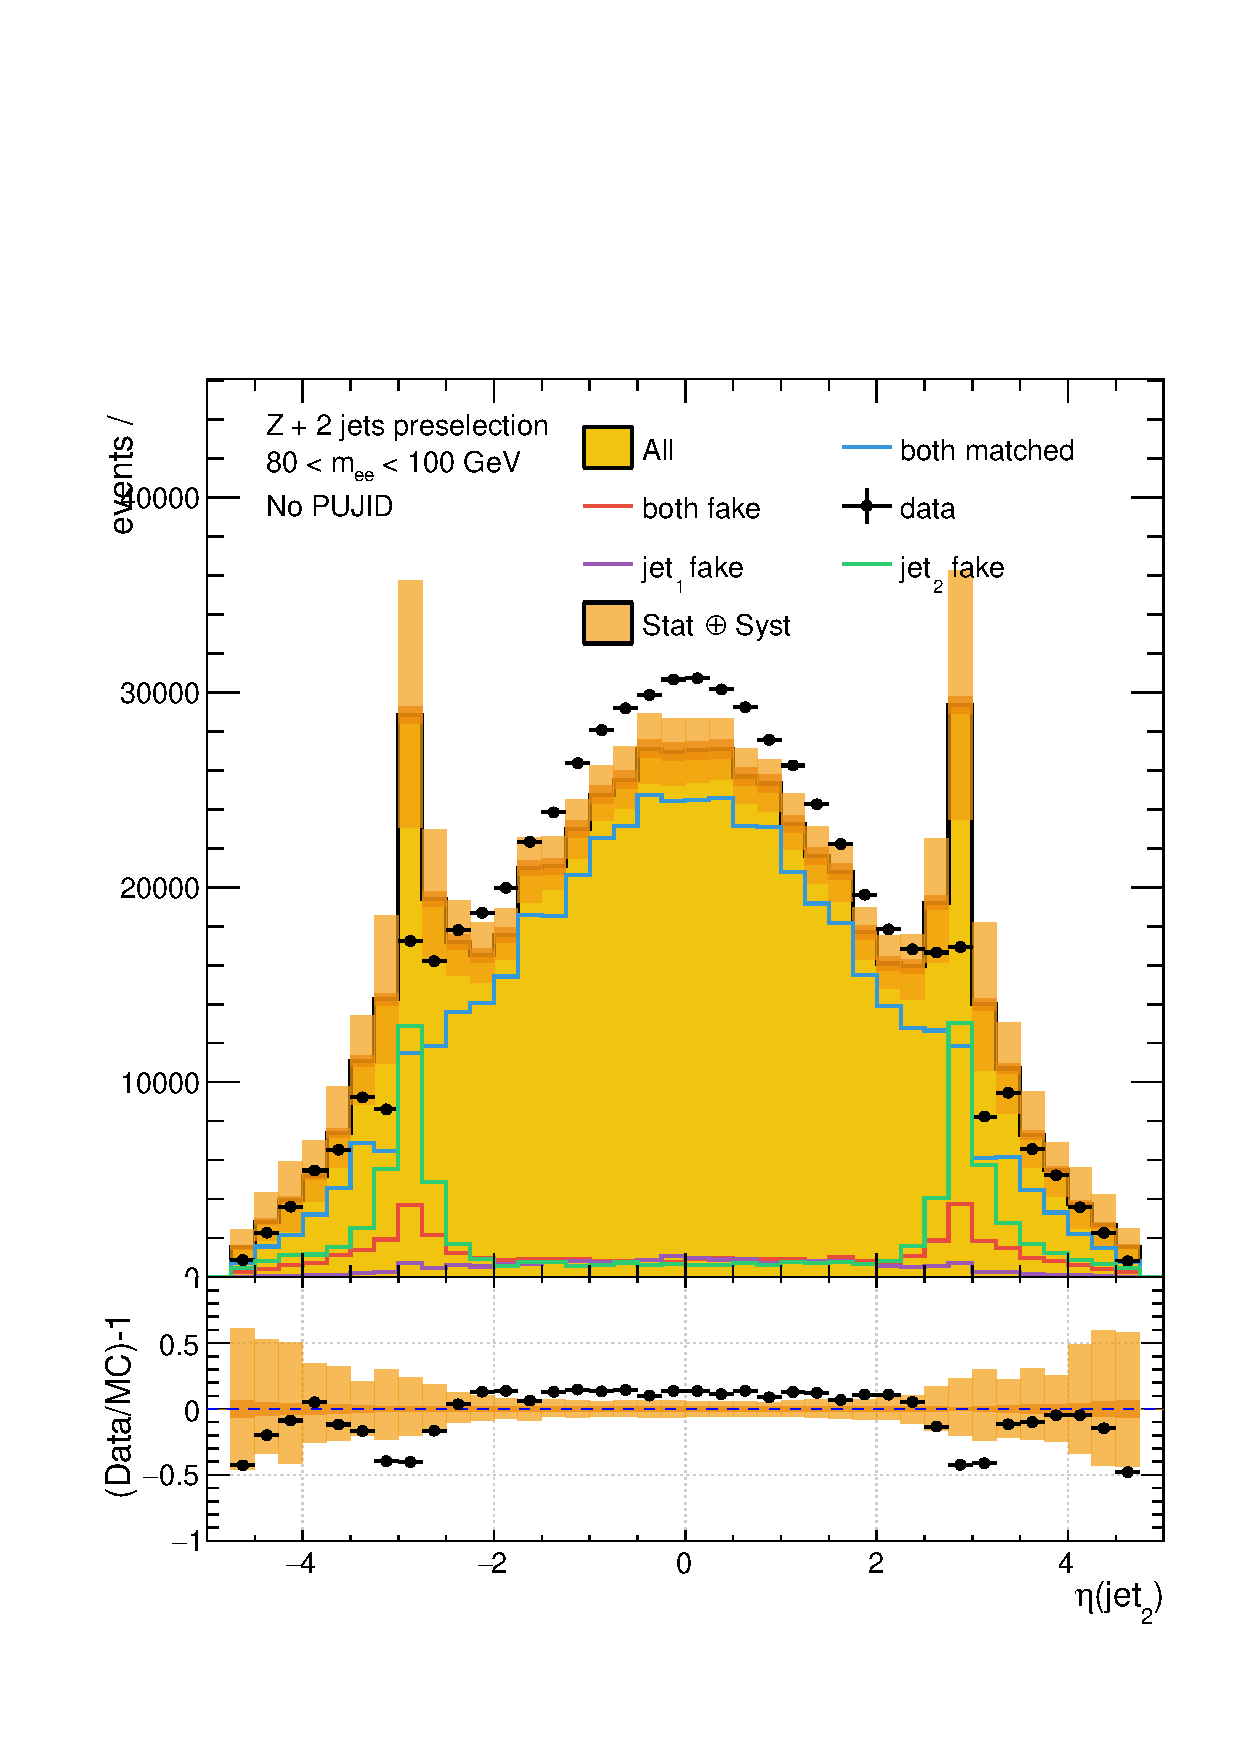
\includegraphics[width=0.45\textwidth]{figures/event_selection/stack_histogram_dijet_subleadEta_zplus2j_none_inclusive_.pdf}
        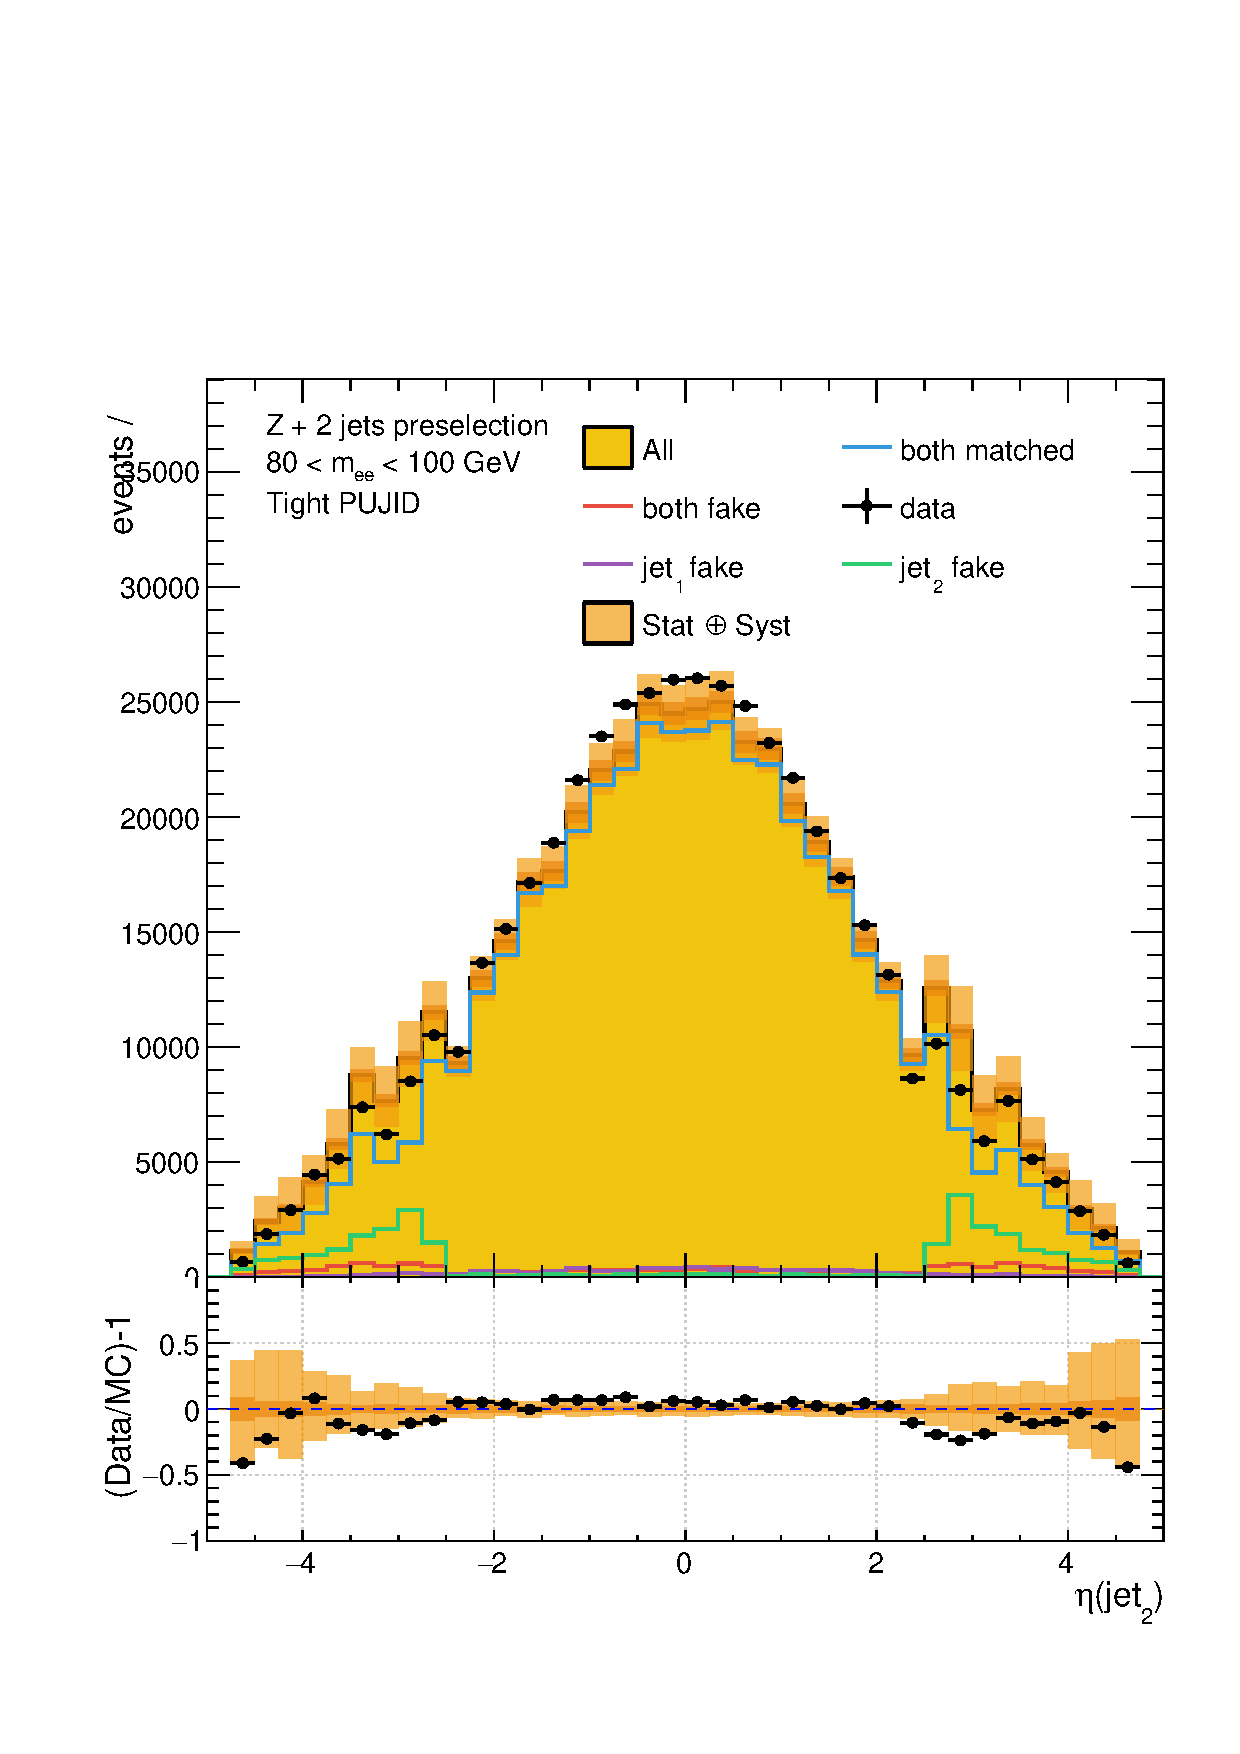
\includegraphics[width=0.45\textwidth]{figures/event_selection/stack_histogram_dijet_subleadEta_zplus2j_tight_inclusive_.pdf}
    \end{center}
    \caption{Sublead pseudorapidity for no PUJID and the tight working point. We note a substantial decrease in fake jets from the endcap/hadronic forward transition region around $|\eta|=3$, and an overall improvement in agreement between simulation and data.}
    \label{fig:event_categorisaton:sublead_eta_pujid}
\end{figure}








\section{VBF Tag: Dense Convolutional Neural Network}
Introduction, mention that the selection is the same, objectives and motivation for the new tag
The objective of the new tag is to use jet images and a dense CNN to enhance VBF signal extraction, especially VBF vs Gluon Fusion discrimination. 


\subsection{Jet Images}
The spatial distribution and properties of a jet's constituent particles contain important discriminating information about the originating parton. 
An image is a natural way of representing this information with the spatial distribution represented by the arrangement of pixel values and the channels of the image representing properties such as charged particle $p_{T}$ in the pixel region.

The image formulation used in this thesis is of two three-channel images stacked in the channels dimension to produce a $n\times{}n\times{}6$ dijet image.
The three channels are the following: $p_T$ deposition of charged candidates, $p_T$ deposition of neutral candidates, and particle multiplicity.
The space that the pixels correspond to is the space of particle displacements in pseudorapidity and azimuthal angle from the jet axis $(\Delta\eta,\Delta\phi)$,
\begin{equation}
    \begin{split}
        \Delta\eta =& \eta_{p} - \eta_{j} \\ 
        \Delta\phi =& \phi_{p} - \phi_{j} \\
    \end{split}
    \label{eq:event_categorisation:pixel_coords}
\end{equation}
where subscript $p$ denotes a constituent particle and $j$ denotes the jet. 
The pixels themselves are not a recilinear grid in $(\Delta\eta,\Delta\phi)$, but are evenly-spaced in the polar coordinates 
\begin{equation}
    \begin{split}
        \Delta{R} =& \sqrt{\Delta\eta^2 + \Delta\phi^2} \\
        \varphi   =& \mathrm{tan}(\Delta\phi/\Delta\eta) \\
    \end{split}
    \label{eq:event_categorisation:pixel_coords}
\end{equation}
These have been rotated by half a pixel in $\varphi$ so that the $(\Delta\eta,\Delta\phi)$ axes line up with the centres of a row of pixels rather than the boundary between them. 
Finally, the images are normalised such that the sum of the $p_T$-based channels equal one, and the sum of the individual multiplicity channels equal one. 
The image formulation is summarised in Figure \ref{fig:event_categorisation:jet_image}.

These images are different in their formulation and behaviour compared to a typical images.
Firstly, they are sparse with only a fraction of the pixels ever active in any one image. 
Secondly, assumptions about local correlations between pixels do not apply: two adjacent red pixels would mean two adjacent particles. Max pooling will simply pick the higher valued pixel during downsampling and information about the second particle will be lost. 
Thirdly, in the rectilinear image which is seen by the network (bottom right of Figure \ref{fig:event_categorisation:jet_image}) there is a periodic boundary condition where the top pixels wrap around to the bottom ones. When convolution operations are performed on these images the padding must be periodic in the vertical direction ($\varphi$ direction).






\newpage
\begin{figure}[h!]
    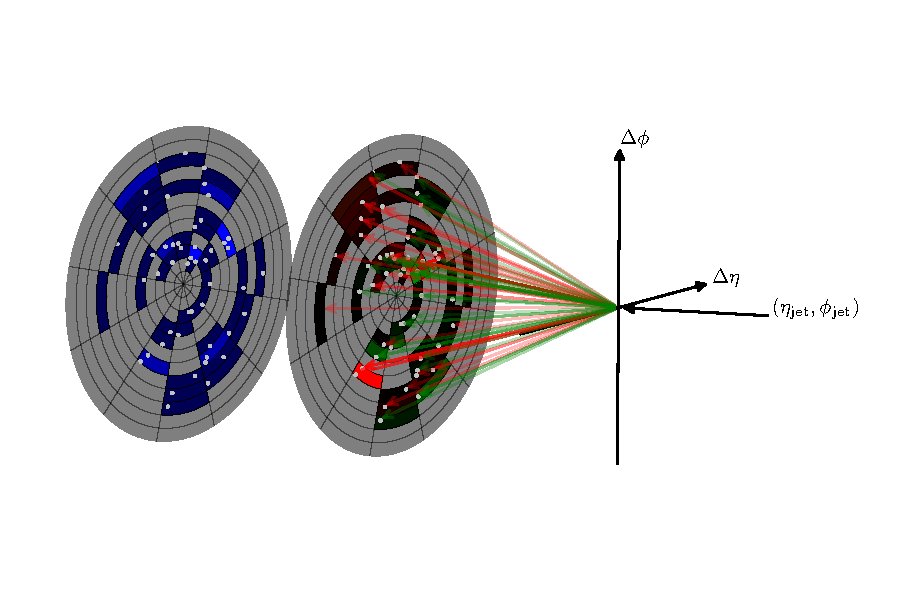
\includegraphics[width=\textwidth]{figures/event_selection/jet_diagram_RGB.pdf}
    \begin{center}
        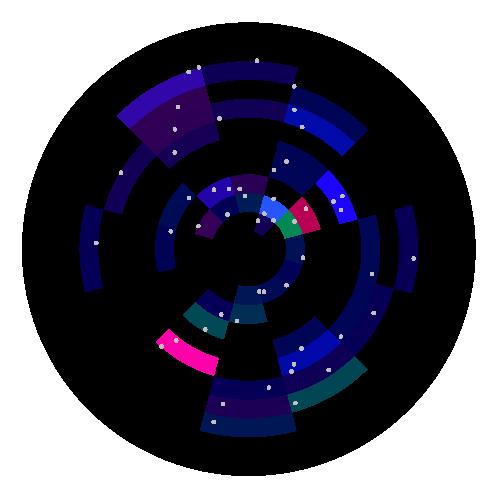
\includegraphics[width=0.49\textwidth]{figures/event_selection/full_image_polar.pdf}
        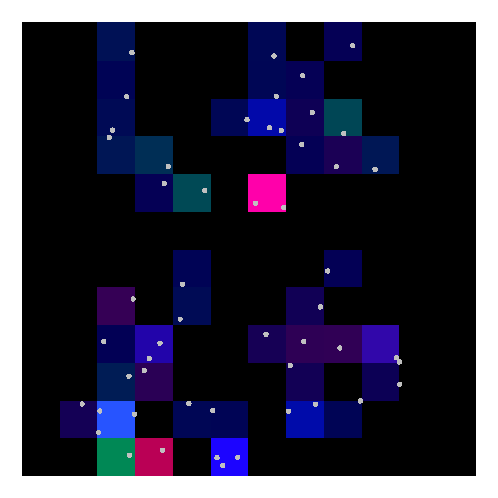
\includegraphics[width=0.49\textwidth]{figures/event_selection/full_image_rect.pdf}
    \end{center}
    \caption{\textbf{Top:} 
             construction of single-jet image from jet constituents. Arrows correspond to individial PF candidates where red arrows are charged, green are neutral and the opacity corresponds to $p_{T}$.
             The red channel measures charged candidate $p_T$ deposition in each pixel, 
             the green channel is neutral charged candidates $p_T$ deposition, 
             and the blue channel is the number of candidates in each pixel (multiplicity). 
             Multiplicity channel is drawn separately so the charged and neutral channels can be seen clearly. Black pixels are lightened to show coloured pixels more clearly.\\
             \textbf{Bottom:} 
             the final image with all the channels together.}
    \label{fig:event_categorisation:jet_image}
\end{figure}



\subsection{Model Design}

The overall structure of the model can be considered to built from three main parts:
\begin{itemize}[leftmargin=.5in,noitemsep]
    \item \textbf{Convolutional section} for learning dijet substructure features from dijet images.
    \item \textbf{Merge section} for processing and integrating engineered kinematic features with learned features from the convolutional section.
    \item \textbf{Main discriminant} fully-connected layers for integrating all information and producing the class logits.
\end{itemize}


The convolutional section consists of a `spread layer' followed by three dense blocks each of which are followed by transition units.

The spread layer is a depthwise convolution layer which produces $N$-many featuremaps for each channel where the filters do not mix the image channels. 
For each channel's associated feature maps half of them have their values evenly permuted in the vertical direction, this corresponds to a rotation by $\pi$ in the polar image.
The function of this layer is to spread out the sparse image into a collection of featuremaps which correspond to simple local spatial configurations of pixels such as radial or angular bands of deposition. 
The interleaved rotations of this layer's output featuremaps allows for the comparison of pixels opposite each other around the jet axis much earlier in the network.  
This layer gives two hyperparameters to the model: the filter size and the number of features per input channel.

The dense blocks construct increasingly higher-level featuremaps, and the transition units will combine feature maps for feature reduction as well as downsampling with average pooling to avoid information loss associated with max pooling mentioned before.  
The structure of each of these parts is tuneable, and therefore gives another twelve hyperparameters to the model: three from each dense block and one from each transition unit. 

The merge section consists of a set of fully-connected layers with the first one after the initial input a different size to the others, this is then concatenated with the output of the convolutional part.
The function of this section is to embed the engineered features in a higher-dimensional space, form them into a vector the same size as the convolutional section output, and then combine them together with the jet structure features. This section has three hyperparameters: the size of the hidden layers, the number of layers, and the size of the first hidden layer relative to the others. 


The main discriminant consists of a sequence of fully-connected layers which take the full vector of concatenated features as input and produce three class logits which correspond to the VBF, ggH, and background process classes. 
These logits are then mapped to class probabilities by a softmax function, the VBF class probability is then used to define tag categories. 

\subsection{Dataset, Training and Loss}
(The loss for training, explain weights as a misclassification cost)
(Cost sensitivity: intra class and inter class costs)
The loss function used is a weighted version of cross entropy where the loss over the minibatch is a weighted mean. For each batch the optimiser will descend the weighted mean of the gradients for each example in the minibatch. The weights are normalised per class so each class has the same total weight, but the shape of their distribution is preserved.  


The optimiser is Adam with nesterov momentum with a learning rate of $0.0001$, slower than the default to ensure smoother filters. 

All of the input features are preprocessed with mean-subtraction and division by their standard deviation. The means and standard deviations are calculated from the training set and these values are applied to the validation and test sets as well as the training set. 
The the training data are augmented by randomly reflecting the images in the $\Delta\eta$ and $\Delta\phi$ directions during training. 

(The regularisation)
The model is regularised with $L_2$ throughout, but with separate values for the different sections. There is also dropout applied to the fully-connected layers during training. 
Dropout is not applied to the convolutional part. 


\subsection{Neural Architecture Search}
Network architecture optimisation

The final model post-opt 

(table of values)

\subsection{Regularization}
Now control the model capactity with regularisation. 

\subsection{Final Model Performance and Categorisation}
The performance of the final model with comparison to the legacy

\subsection{Learned Features Interpretation}
We would like to figure out what sort of features the convolutional section is forming. There are three approaches we will explore here: maximally activating images from the dataset, image occlusion studies, and the production of maximally activating images using stochastic gradient descent (deep dreams).  


\section{Untagged}
If the candidate does not receive a tag it is conisdered for the untagged categories which make a selection diphoton BDT score. These categories mostly consist of gluon fusion events. 




    
\chapter{Statistical Analysis and Results}
\label{chap:statistical}

%\newpage

\section{Introduction}
The set of categorised diphoton candidates are subjected to a statistical interpretation to measure the Higgs boson signal in data and to determine how its properties compare to SM expectations.
This procedure consists of a statistical model that is fitted simultaneously to the \mgg distribution in data for each tag category. 
Separate models are constructed and then combined for signal and background that take into account the contribution of different categories, production modes and systematic uncertainties.

This chapter begins by describing the construction of these models and the inclusion of the associated systematic uncertainties (following \cite{HIG-16-040}). 
After this, the final fit of the model and the statistical interpretation of the result is described with emphasis on how the two different VBF tagging approaches affect the result. 


\section{Statistical Models}
\subsection{Signal Modelling}
The signal modelling aims to construct a signal shape for each category using simulated data samples of the different Higgs production modes.
This is achieved by constructing many parameterised signal shapes: one for each choice of production mode, category and whether the vertex has been correctly identified. 

Furthermore, the Higgs boson mass \mH is not assumed to have a specific value. A parameterisation of the signal shape in terms of \mH is derived from a collection of samples with different \mH.
This is constructed by performing a simultaneous fit over all of the mass points where the parameters of the signal shape are all polynomials of \mH. 
The floating parameters of this fit are then the coefficients of the polynomial. 
This approach is used instead of interpolating the parameters as it leads to fewer parameters per fit and guarantees consistency across mass points. 

This procedure is also used to determine relative normalisation of the RV and WV scenario shapes when they are combined. 
This is given by the vertex selection efficiency derived from simulated data. 
The value is then treated the same way as the other shape parameters in the simultaneous mass point fit. 

Once constructed the different signal shapes from production modes are combined together to produce the signal model for each category. 
The production mode shapes are normalised to their expected signal yield and then summed.



\subsection{Background Modelling}
The background modelling aims to construct a smoothly falling background distribution that takes uncertainty about the choice of functional form into account. This is achieved with a data-driven approach based on the discrete profiling method \cite{env_method}. This technique allows for the estimation of this systematic and its propagation to the final fits as a discrete nuisance parameter without assumptions about underlying processes or functional forms. 

The candidate functions are expressed as a set of function families, each of these are expressed as a sequence where we pick a lowest and highest order form to consider. The maximum order is found via an F-test and the minimum order is found by requiring a minimal level of goodness-of-fit. 
The families considered are polynomials in the Bernstein basis, Laurent series, sums of exponentials, and sums of power laws. 

The functions are fitted to the \mgg sideband data using twice negative likelihood (2NLL) minimisation with an additional regularisation term $n_p$ (number of parameters) to penalise function complexity. 



\section{Systematic Uncertainties}
Systematic uncertainties are propagated to the final fits by including nuisance parameters primarily in the signal model. 
The desription here is taken from the work in \cite{HIG-16-040} unless stated otherwise. 

Systematic error in the signal model is handled in one of three main ways via nuisance parameters that have different effects on the \mgg distribution:
\begin{itemize}[noitemsep]
    \item Shape uncertainties are propagated via nuisance parameters that alter the shape of the Gaussian signal peak position, width and normalisation.
    \item Yield uncertainties are handled by nuisance parameters that scale the \mgg distribution and are subject to a log-normal constraint during the final fit.
    \item Categorisation uncertainties are implemented as category migration nuisance parameters which behave in a similar way to yield uncertainties but will reduce yield in other categories simultaneously as the category of interest is increased.
\end{itemize}
There is an exception to this scheme with the vertex uncertainty. Here there is a nuisance parameter that controls the relative fraction of the RV/WV signal distributions. 

An extra systematic uncertainty from choice of background functional form is propagated to the final fits via the background model as a discrete nuisance parameter. 



\subsection{Theoretical Uncertainties}
Uncertainties from QCD theory calculations have their effect modelled in two ways: uncertainty on the overall yield for a process and uncertainty associated with analysis category migration. 
The migration uncertainties extracted separately by scaling such that the overall yield is unchanged.  
\begin{itemize}[noitemsep]
    \item {\textbf{QCD scale uncertainty}: yield uncertainty is parameterised separately for renormalisation scale and factorisation scale. 
                                            Category migrations associated with varying these parameters independently and together are also included.}
    \item{\textbf{PDF uncertainties}: There is an uncertainty associated with variation in the signal yield of each production process, and category migration uncertainties.   
        The yield uncertainty is calculated using the procedure from PDF4LHC \cite{PDF4LHC} and the migration uncertainties are computed from the NNPDF3.0 PDF set \cite{NNPDF3} and the MC2Hessian \cite{MC2Hessian} procedure.}
    \item{\textbf{Strong force coupling ($\alpha_{s}$) uncertainty}: evaluated with the same procedure as the PDF uncertainties.}
    \item{\textbf{Underlying event and parton shower uncertainty}: evaluated using simulated data where the modelling of the underlying event and the parton showers have been varied. This manifests primarily as variation in the jets of the analysis and is modelled as a category migration uncertainty. The probability that events move within the categories of the VBF tag, or from the VBF tag to Untagged are found to be 7 and 9\%. This was re-evaluated for the DCNN-based VBF tag and found to be unchanged.}
    \item{\textbf{Gluon fusion contamination in \ttH tag categories}: when the Higgs boson is produced by ggH it can be produced in association with a number of jets. As the number of jets becomes large the accuracy of theoretical predictions becomes worse and introduces a systematic uncertainty in ggH contamination of the jet-based tag categories. This manifests in the \ttH tags in multiple ways:
        \begin{itemize}[noitemsep]
            \item[\textbullet] \textbf{Uncertainty due to limited ggH sample size}: only a small quantity of simulated ggH events are accepted into the \ttH tag. This introduces a significant statistical uncertainty on the ggH yield and contributes a 10\% uncertainty.
            \item[\textbullet] \textbf{Uncertainty due to modelling parton showers}: this is estimated by comparing simulation and data for events whose production is dominated by gluon-fusion-type diagrams ($\mathrm{t}\bar{\mathrm{t}}+\mathrm{jets}$ with semi-leptonic $\mathrm{t}\bar{\mathrm{t}}$ decays) binned by the number of jets. The largest discrepancy is in $N_{\mathrm{jets}}\geq{5}$ which corresponds to an uncertainty of 35\%.
            \item[\textbullet] \textbf{Uncertainty due to modelling gluon splitting}: estimated by calculating the difference in the ratio $\sigma(\mathrm{t\bar{t}b\bar{b}})/\sigma(\mathrm{t\bar{t}jj})$ for simulation and data. The fraction of events in simulated ggH with b jets are then scaled by this difference. This gives a 50\% variation in the ggH yield for the \ttH tags. 
        \end{itemize}}
    \item{\textbf{Gluon fusion contamination in tag categories with jets and a high-\pt Higgs boson}: how ggH mismodelling manifests in the VBF categories in particular:
        \begin{itemize}[noitemsep]
            \item[\textbullet] \textbf{Uncertainty due to jet multiplicity mismodelling}: two nuisance parameters due to missing higher-order terms and two more nuisance parameters for category migration due to variation in jet multiplicity based on STWZ \cite{JetPtResum} and BLPTW \cite{JetPtResum,TheoryUncertHiggs1J,ResummedHiggsPredictions} predictions. 
            \item[\textbullet] \textbf{Uncertainty due to Higgs boson \pt mismodelling}: two nuisance parameters associated with migration between two bins in Higgs boson \pt; from 60 to 120 \,GeV and above 120\,GeV. There is also a third nuisance due to uncertainty in top quark mass effects. This is negligible for \pt less than 150\,GeV but increases to 35\% at 500\,GeV. These impact the highest-score VBF and Untagged categories where the ggH yield uncertainty is 6-8\%.
            \item[\textbullet] \textbf{Uncertainty in the acceptance of ggH in VBF categories due to QCD effects}: effects from missing higher-order terms are estimated via variations in the renormalisation and factorisation scales in MCFM 5.8 \cite{MCFM}. Two nuisance parameters are introduced associated with the overall normalisation of Higgs bosons produced in association with two jets, and three or more jets. This allows for the impact of jet suppression arising from how the kinematic variables are used to form the VBF scores to be propagated to the analysis. The procedure is based on the Stewart-Tackmann method \cite{StewartTackmann,GangalTackmann} and the impact on the ggH yield in the VBF categories is 8-13\%. 
        \end{itemize}}
    \item{\textbf{Uncertainty in the \Hgg branching fraction}: the uncertainty on the theoretical prediction of the \Hgg branching fraction is taken from \cite{LHCHXS} and is approximately 2\%.}
\end{itemize}

The theory uncertainties with the largest impact on measuring signal strengths and couplings are the \Hgg branching fraction; and the renormalisation and factorisation scale uncertainties from the QCD scale. 



\subsection{Experimental Uncertainties}
Uncertainty in the measurement and construction of physics objects at CMS give rises to associated experimental systematic uncertainties. 
These affect the shape of the signal distribution and are propagated through to the final fits via the signal model. 
\subsubsection{Photon Energy Measurement Uncertainties}
Uncertainties in the photon energy measurement are a particularly important contribution and can affect the signal shape via both the photon energy scale and resolution.
\begin{itemize}[noitemsep]
    \item {\textbf{Energy scale and resolution}: 
           uncertainties associated with the photon energy scale and resolution corrections
           are estimated with events from the \Zee control region reconstructed as photons. Data and simulation are compared in eight bins of $R_9$ and $|\eta|$ (high/low-$R_9$, and four $|\eta|$ bins). 
           The uncertainties are quantified separately in four photon classes (EB/EE and high/low-$R_9$) and are propagated to the categorisation with four scale nuisance parameters (one per photon class) and eight shape nuisance parameters (one constant and one stochastic term per photon class) for each event category. 
           This has a 0.15-0.5\% effect on the photon energy, and an effect of 2.5\% on the signal strength modifier. 
           }
    \item {\textbf{Nonlinearity of photon energy}: 
          There is potential residual data-simulation difference in the linearity of the ECAL response with photon energy scale. 
          This is estimated by studying boosted \Zee events and has the effect of shifting the peak position by a small amount per category, constituting a maximum uncertainty of 0.1\% in each category except for the untagged where it is 0.2\%. The uncertainty is propagated to the final fits as a shape nuisance parameter that shifts the signal peak position.
          }
    \item {\textbf{Non-uniformity of light collection}: 
           There is a systematic uncertainty associated with the modelling of the fraction of scintillation light reaching the ECAL crystal photodetector as a function of the longitudinal depth of the shower start. The size of this effect is 0.07\% on the photon energy scale.
           }
    \item {\textbf{Electromagnetic shower modelling}: 
        Mismodelling of electromagnetic showers in \texttt{GEANT4} introduces a small difference between electrons and photons and therefore another small uncertainty. 
           It is estimated by comparing the latest version of shower simulation with a previous one and treating the small difference between them as representing the limit of accurate modelling. 
           This gives a contribution of 0.05\% uncertainty to the photon energy scale.
           }
    \item {\textbf{Modelling of the material budget}: 
           The amount of material between the interaction point and the ECAL affects the behaviour of photons and electrons. 
           The modelling of this material is a further source of systematic uncertainty. 
           This uncertainty is estimated using simulated samples where the material has been uniformly varied by $\pm5\%$ to cover the difference in the estimation between simulation and data.
           The uncertainty manifests as an effect on the photon energy scale of 0.24\%.
           }
    \item {\textbf{Shower shape corrections}: 
           Finally, there is an uncertainty due to mismodelling of shower shapes themselves. This is estimated by comparing between simulation samples with and without corrections on shower shape variables. This gives an uncertainty in the photon energy scale of 0.01-0.15\% at maximum. This is propagated by separate signal shape nuisance parameters for each photon category.  
           }
\end{itemize}

\subsubsection{Additional Experimental Uncertainties}
Additional uncertainties that are not directly from the photon measurement arise from estimations of efficiencies, scale factors and selection variables. These are varied and their estimated effects propagated through the analysis chain. They are then applied as per-category yield and category migration nuisance parameters in the final fits. 
\begin{itemize}[noitemsep]
    \item {\textbf{Trigger efficiency}: 
           uncertainty in the trigger efficiency estimation is evaluated with the \Zee control region and the tag-and-probe technique. This leads to an impact on the event yields of 0.1\% at maximum.}
    \item {\textbf{Photon preselection}: 
           the uncertainty of the photon preselection efficiency is estimated as the ratio between the efficiency measured in simulation and data. This has an impact on event yields of 0.2-0.5\% depending on category.}
    \item {\textbf{Photon ID BDT score}: 
           Photon energy measurement uncertainties are propagated through the categorisation process to estimate their effect on category signal yields via the photon ID. The uncertainty is assigned to cover the observed difference between data and simulation in the \Zee control region. 
           }
    \item {\textbf{Photon energy resolution estimation}: 
        This uncertainty is estimated by rescaling the energy resolution estimate around its nominal value by $\pm{5}\%$ to cover all disagreement between data and simulation. This variation is propagated through the categorisation and is implemented as a yield nuisance parameter. 
           }
    \item {\textbf{Jet energy scale and smearing corrections}: 
           Uncertainties in the correction of jet energy measurements are propagated through the event categorisation and are modelled as category migration nuisance parameters. 
           These nuisance parameters correspond to migration within VBF categories, within VH categories, within \ttH categories and from these tags to the Untagged categories. 
           Jet energy scale corrections correspond to the following migrations: 
           \begin{itemize}[noitemsep]
               \item[\textbullet] 8-11\% between VBF categories and 11\% from VBF to Untagged;
               \item[\textbullet] 15\% from VH to Untagged;
               \item[\textbullet] 5\% from \ttH to Untagged.
           \end{itemize}
           The jet energy resolution has a migration effect of at most 3\% across all tags except for VH where it can reach 20\%.
           }
    \item {\textbf{Missing transverse energy}: 
           uncertainty in the measurement of \MET is estimated by varying the \pt of reconstructed physics objects entering the calculation of \MET for the event. 
           These variations correspond to the momentum scale and resolution uncertainties of each type of physics object. 
           This is correspond to a 10-15\% migration between Untagged and VH MET and is propagated to the final fits as a category migration nuisance.
           }
    \item {\textbf{Pileup jet ID}: 
           uncertainty associated with the PUJID in the VBF tags is analysed using \Zee events with one jet whose momentum balances the dielectron in the transverse plane.            
           Data and simulation are compared and the disagreement is used to estimate VBF category migrations. This effect is found to be at most 1\% and is propagated to the final fits as a category migration nuisance. 
           }
    \item {\textbf{Lepton isolation and ID}: 
           the associated uncertainty is estimated for both electrons and muons by measuring the difference in efficiency between simulation and data and varying an associated scale factor within this difference. 
           This is measured using the tag-and-probe technique on both \Zee and \Zmumu.
           The associated variations manifest as yield uncertainties and are at most 1\% for the \ttH Leptonic category, 1.5\% for the WH Leptonic category and 3\% for the ZH Leptonic category. They are propagated to the final fit as category yield nuisance parameters. 
           }
    \item {\textbf{Efficiency of b-tagging}: 
           this uncertainty is evaluated by comparing data and simulation distributions of the b-tagging discriminant score. The uncertainty has a statistical component associated with the estimation of the relative amount of light and heavy quark initiated jets and confusion between them. 
           This uncertainty is propagated in two different ways due to the difference in approach of the \ttH Hadronic and \ttH Leptonic tags
           \begin{itemize}[noitemsep]
               \item[\textbullet] the hadronic category uses a BDT that receives the b-tagger discriminant score as an input feature. The associated yield uncertainty is evaluated by altering the shape of the score in simulation and found to be at most 5\%.
               \item[\textbullet] the leptonic category uses a fixed selection on the b-tagger discriminant score. This uncertainty is evaluated by varying the efficiency in data and simulation within their uncertainties and is found to be 2\%.  
           \end{itemize}
           }
    \item {\textbf{Vertex finding efficiency}: 
           this uncertainty derives from mismodelling of the underlying event and disagreement between data and simulation from evaluating \Zmumu events. The size of this uncertainty is around 2\% and is propagated to the final fit as a nuisance parameter that changes the relative contribution of the RV and WV signal shapes.
           }
    \item {\textbf{Integrated luminosity}: 
        this uncertainty is taken from \cite{LumiUncert} and modelled as a yield nuisance that affects all processes uniformly. The size of this effect is 2.5\%.
           }
    \item {\textbf{Background modelling}: 
           Handled by the discrete profiling method and propagated to the final fits as a discrete nuisance that picks different functional forms. 
           }
\end{itemize}

The experimental systematic uncertainties with the largest impact on signal strength and couplings measurements are from the photon shower shape corrections which affects the photon ID and the photon energy resolution estimate; the photon energy scale and smearing; the jet energy scale; and the integrated luminosity.









\section{Results}
Different measurements are extracted by performing a series of fits to the \mgg distributions simultaneously across all event categories under different constraints. 
The fits are carried out in the range $100 < m_{\gamma\gamma} < 180$\,GeV with a binning of 250\,MeV, using a binned maximum-likelihood fit.
The likelihood function to be used is the product of the individual category likelihoods and has the following form:
\begin{equation}
    \mathcal{L}(\mu_{c},m_H,\vec{n}|m_{\gamma\gamma}) = \prod_{c=0}^{N-1} \left( \mu_{c} S_{c}( m_{H}, \vec{n}_{s} | m_{\gamma\gamma}) + B_{c}( \vec{n}_{s} | m_{\gamma\gamma}) \right),
\end{equation}
where $c$ enumerates the $N$-many event categories; $S_{c}$ is the signal model of category $c$; $B_{c}$ is the background model of category $c$; $m_H$ is the Higgs signal peak position; $\vec{n}$ are the nuisance parameters of the model with $\vec{n}_s$ and $\vec{n}_b$ being the nuisance parameters of the signal and background models respectively; and $\mu_{c}$ is the category signal strength. 
The signal strengths are constrained to be the same depending on the measurement being performed: a global $\mu$ fit constrains them all to the same value that then floats in the fit, per-process $\mu$ fits will allow for different values between the production modes, but categories within them will use the same value. 

This is maximised by finding the minimum twice negative log-likelihood (2NLL) of $\mathcal{L}$, 
\begin{equation}
    2\mathrm{NLL} = -2\ln\mathcal{L}(\mu_{c},m_H,\vec{n}|m_{\gamma\gamma}),
\end{equation}
while taking into account constraints on the parameters. 


\subsection{Best Fit of Model to Data}
A maximum-likelihood fit is performed with a single global $\mu$ and $m_H$ to find their best fit values.
These constitute the central values of a measurement of the global $\mu$ and the associated uncertainty is calculated via a likelihood scan of an associated test statistic. 
Example mass fit plots for both BDT and DCNN-based VBF tags are shown in Figure \ref{fig:stats_results:vbf_mass_plots}.
A full set of mass fit plots for BDT-based and DCNN-based VBF tags can be found in Appendix \ref{appendix:mass_plots}.

Expected category yields by production mode contribution are shown in Table \ref{tab:stats_results:yield_table} for fits with the BDT-based and DCNN-based VBF tags. 
A reduction in contamination from ggH is observed in the DCNN-based VBF tag categories, particularly in VBF 0 where it has been reduced by around a third from 15.5\% to 9.5\%. 
Downstream VH tags are only slightly affected, and the overall effect on the inclusive untagged categories is small. 

The effect of using the DCNN-based VBF tag over the BDT-based tag on category significances is shown in Table \ref{tab:stats_results:sig_table}.
An increase in overall expected significance of 13\% is observed in the DCNN-based tag. 
\newpage
\begin{figure}[h!]
    \begin{center}
        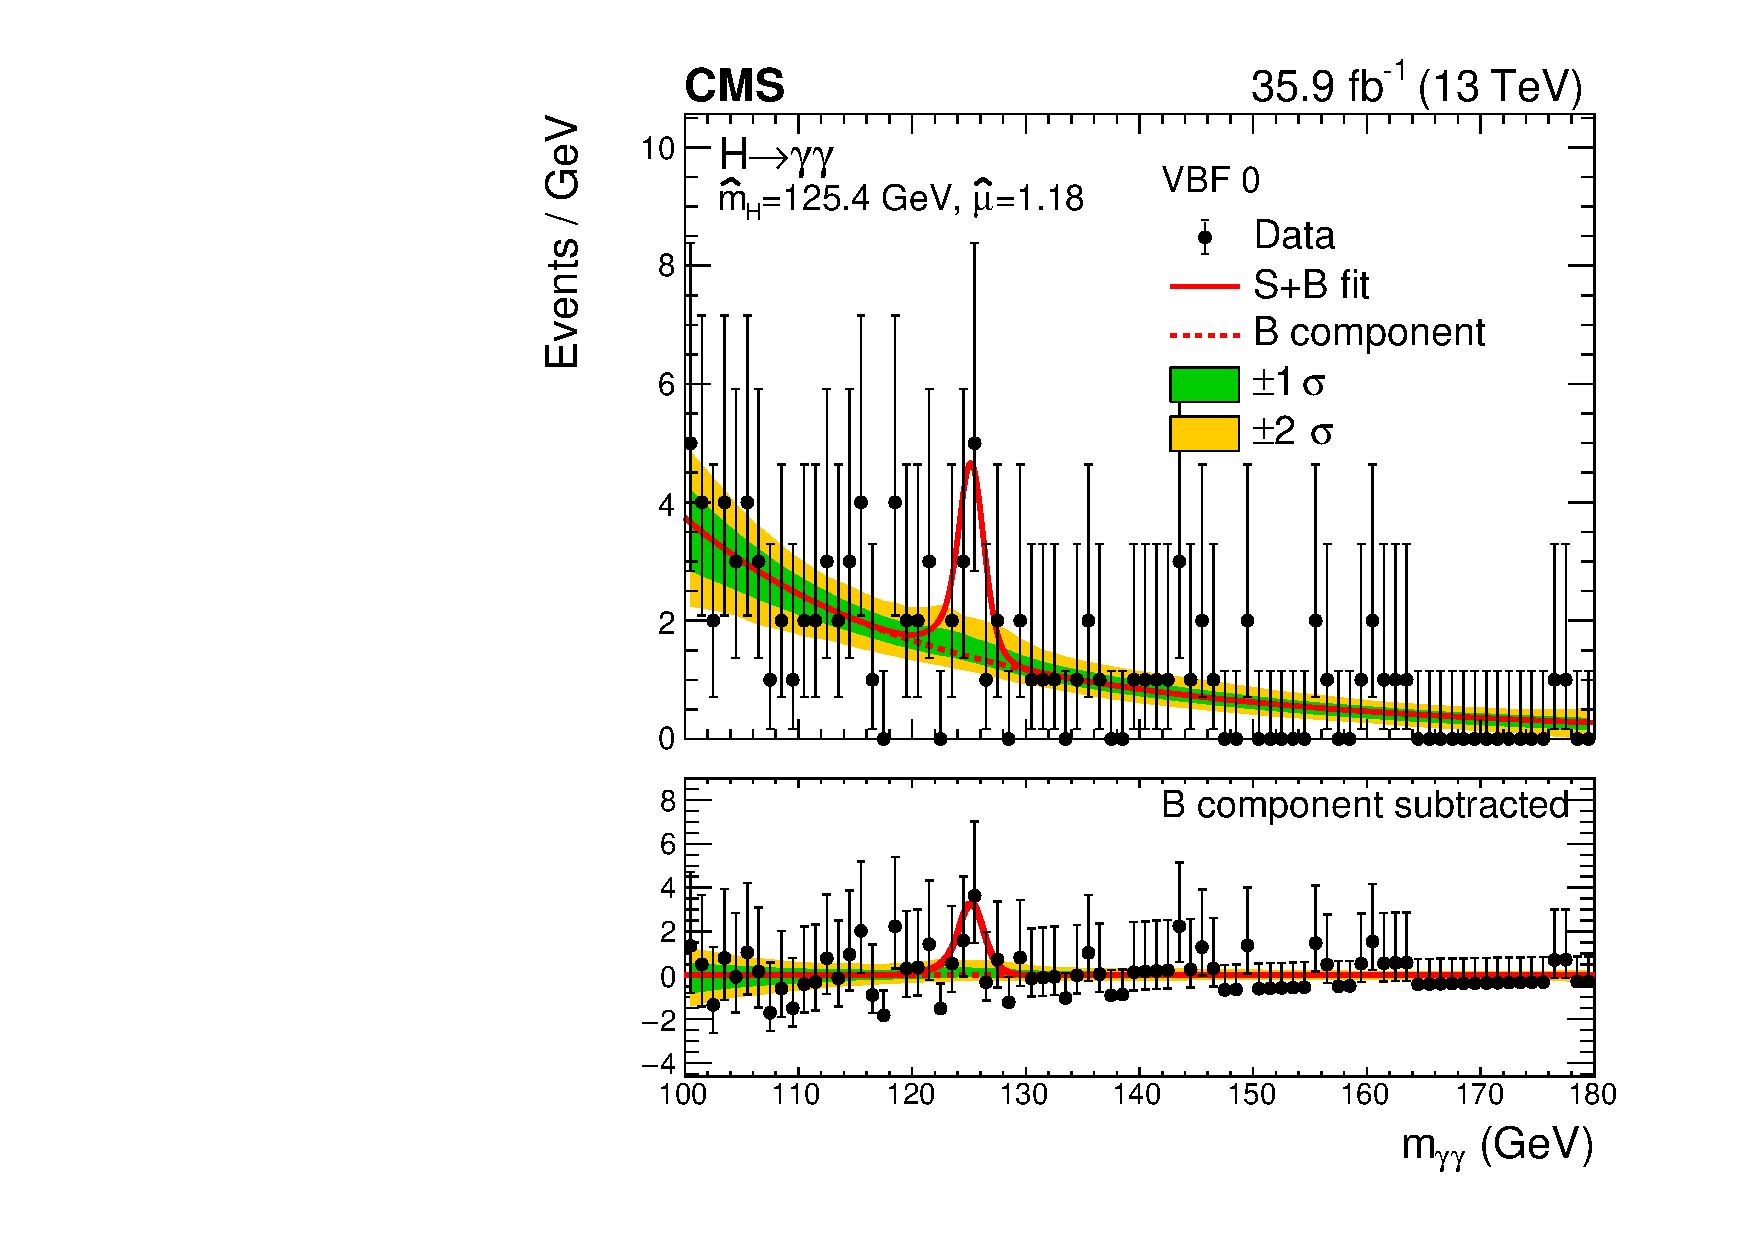
\includegraphics[width=0.47\textwidth]{figures/stats_results/CMS-HIG-16-040_Figure_012-a.pdf}
        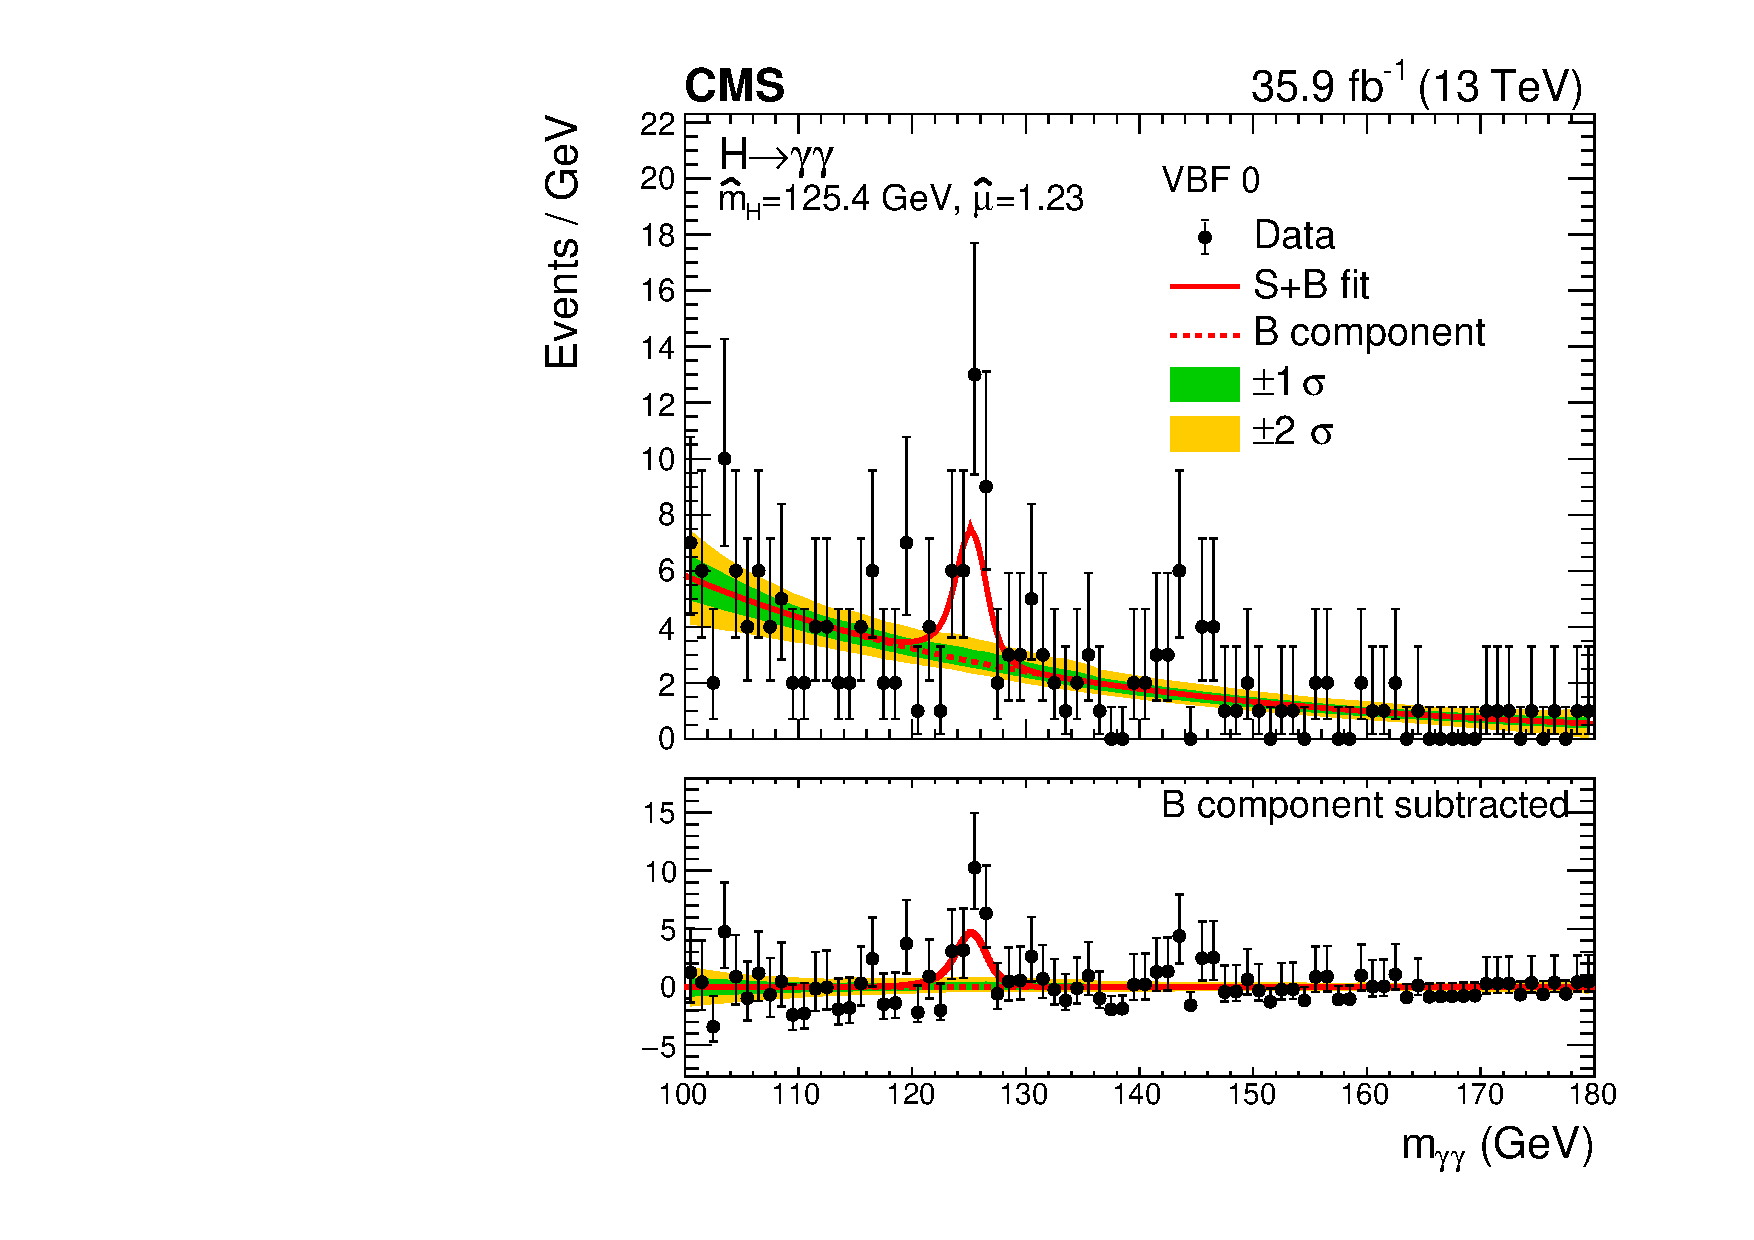
\includegraphics[width=0.47\textwidth]{figures/stats_results/SBplots_jackWSnewVBFTag_0_13TeV.pdf}
    \end{center}
    \begin{center}
        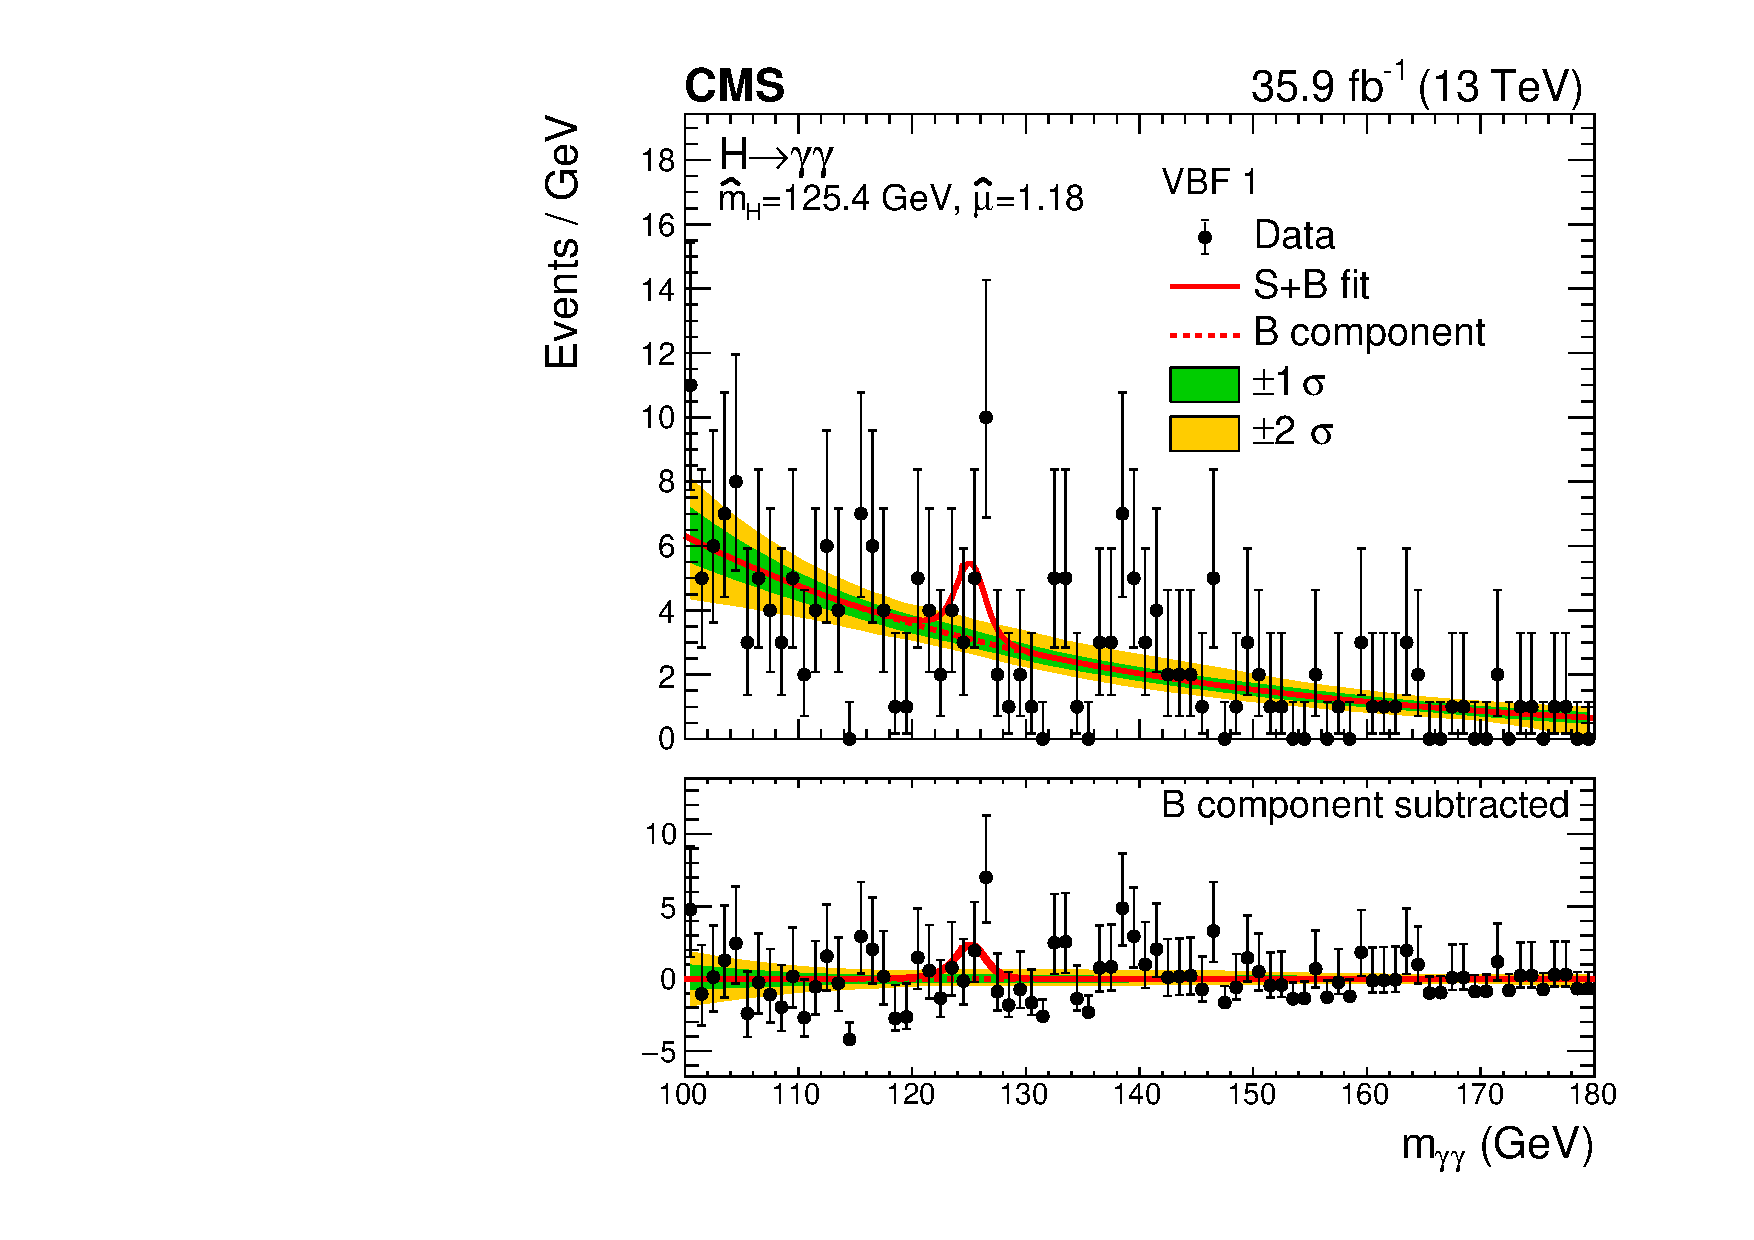
\includegraphics[width=0.47\textwidth]{figures/stats_results/CMS-HIG-16-040_Figure_012-b.pdf}
        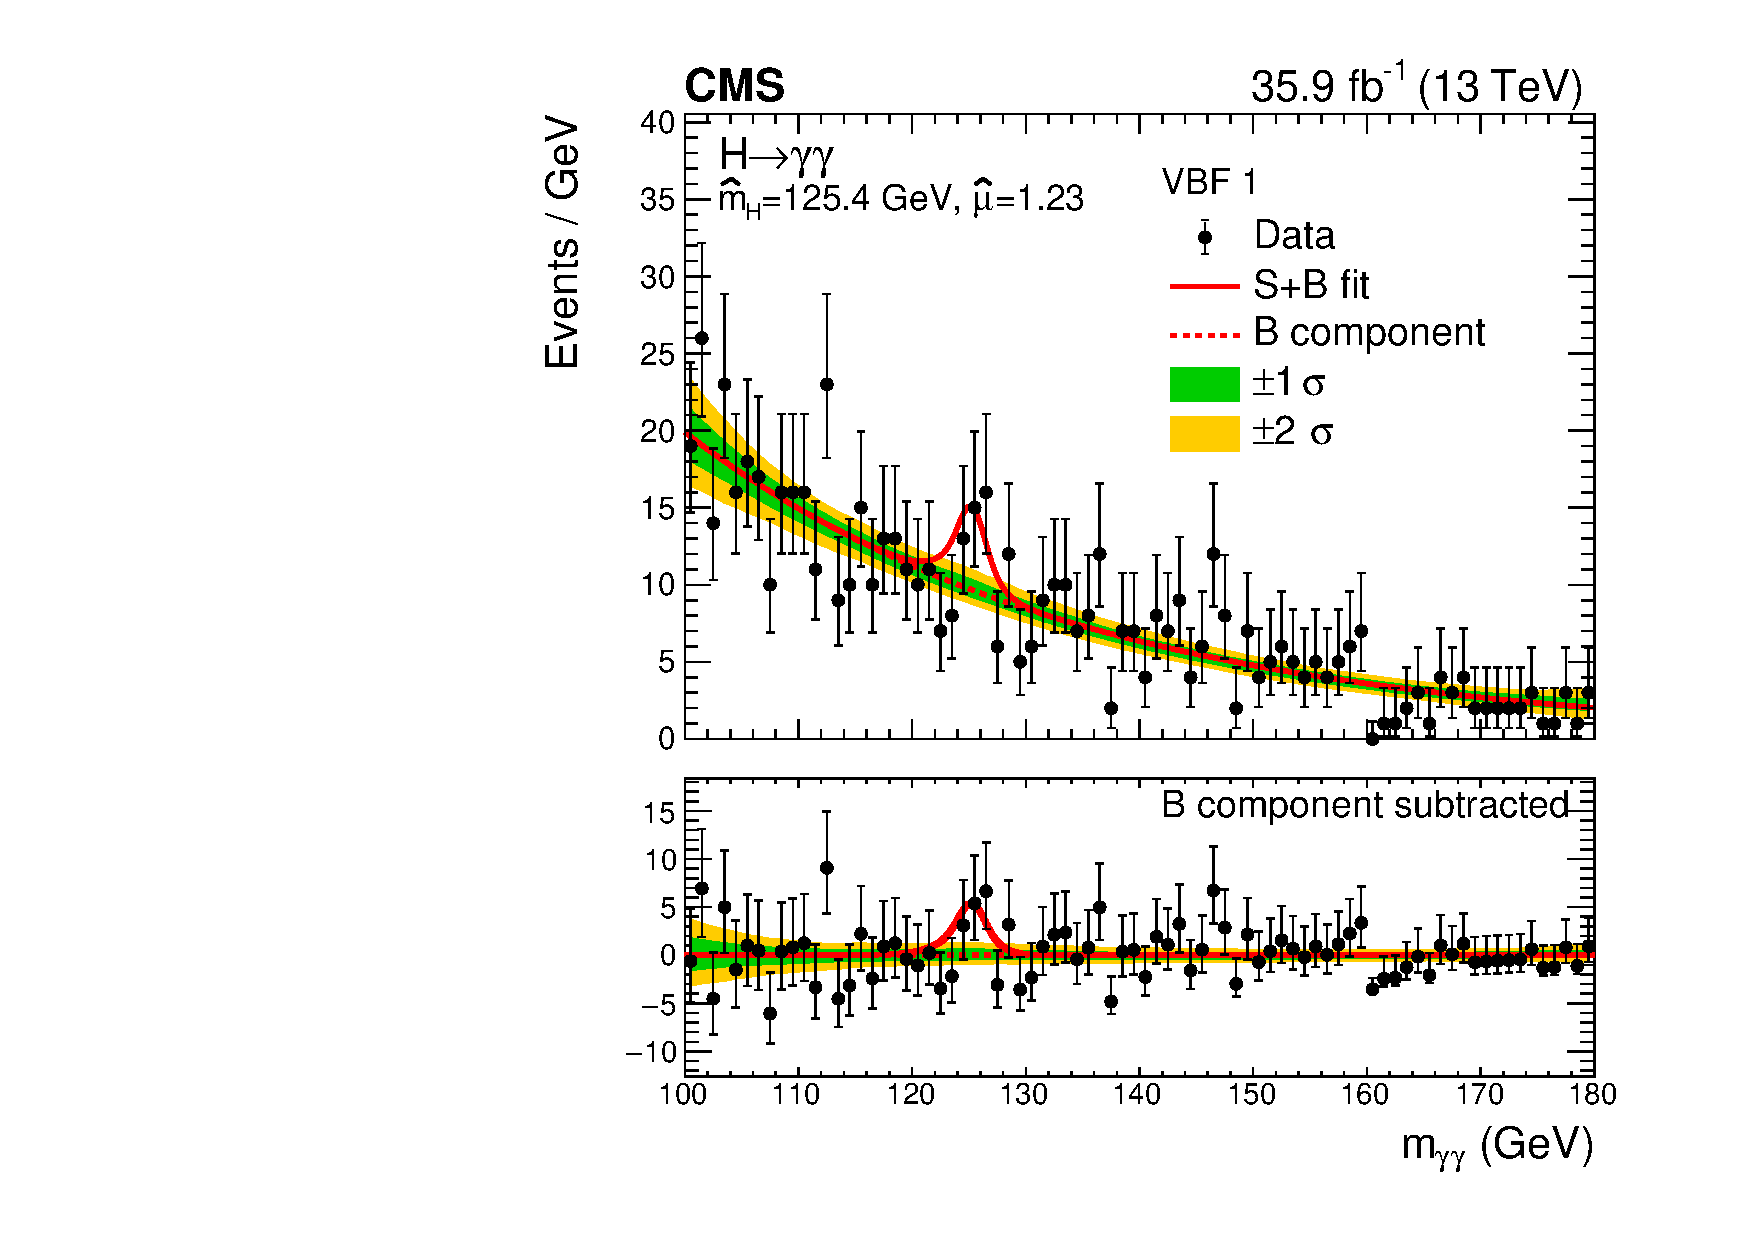
\includegraphics[width=0.47\textwidth]{figures/stats_results/SBplots_jackWSnewVBFTag_1_13TeV.pdf}
    \end{center}
    \begin{center}
        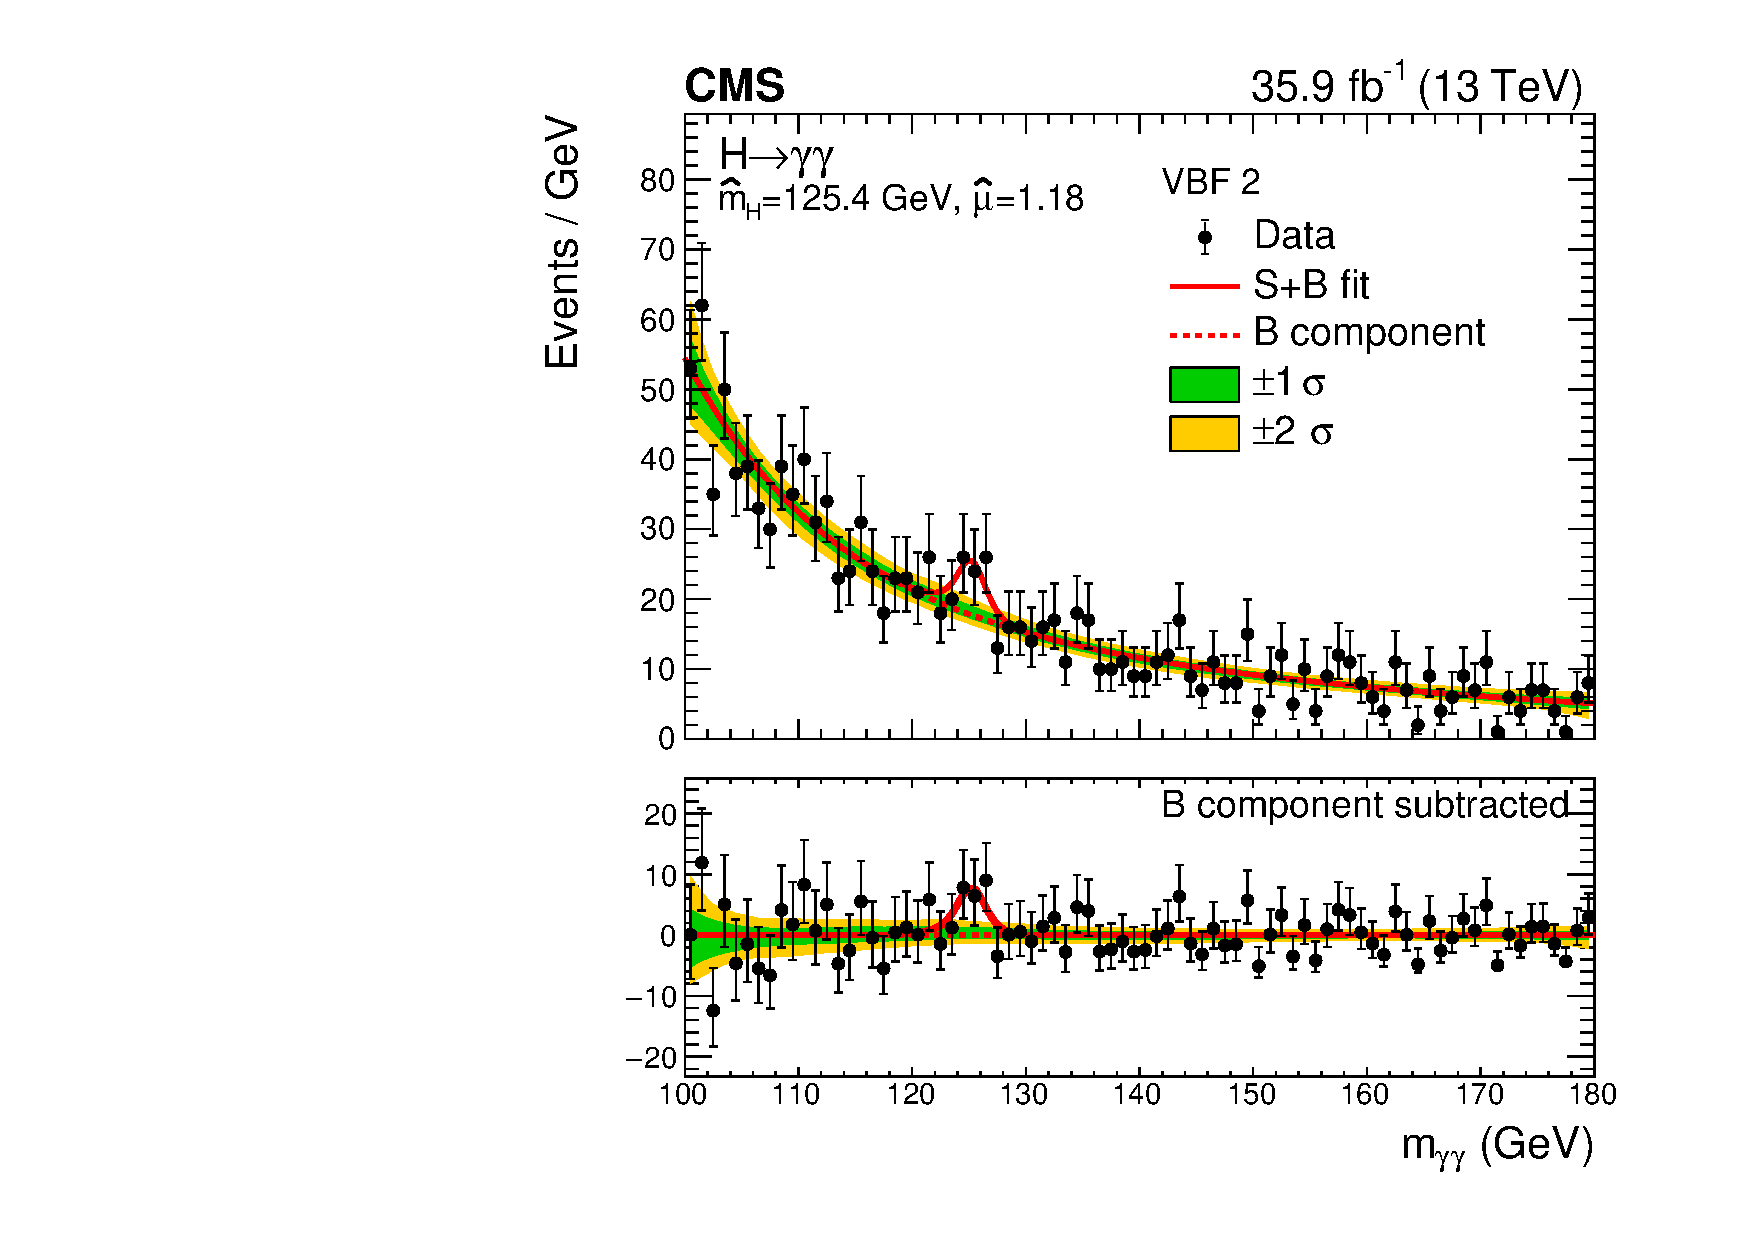
\includegraphics[width=0.47\textwidth]{figures/stats_results/CMS-HIG-16-040_Figure_012-c.pdf}
        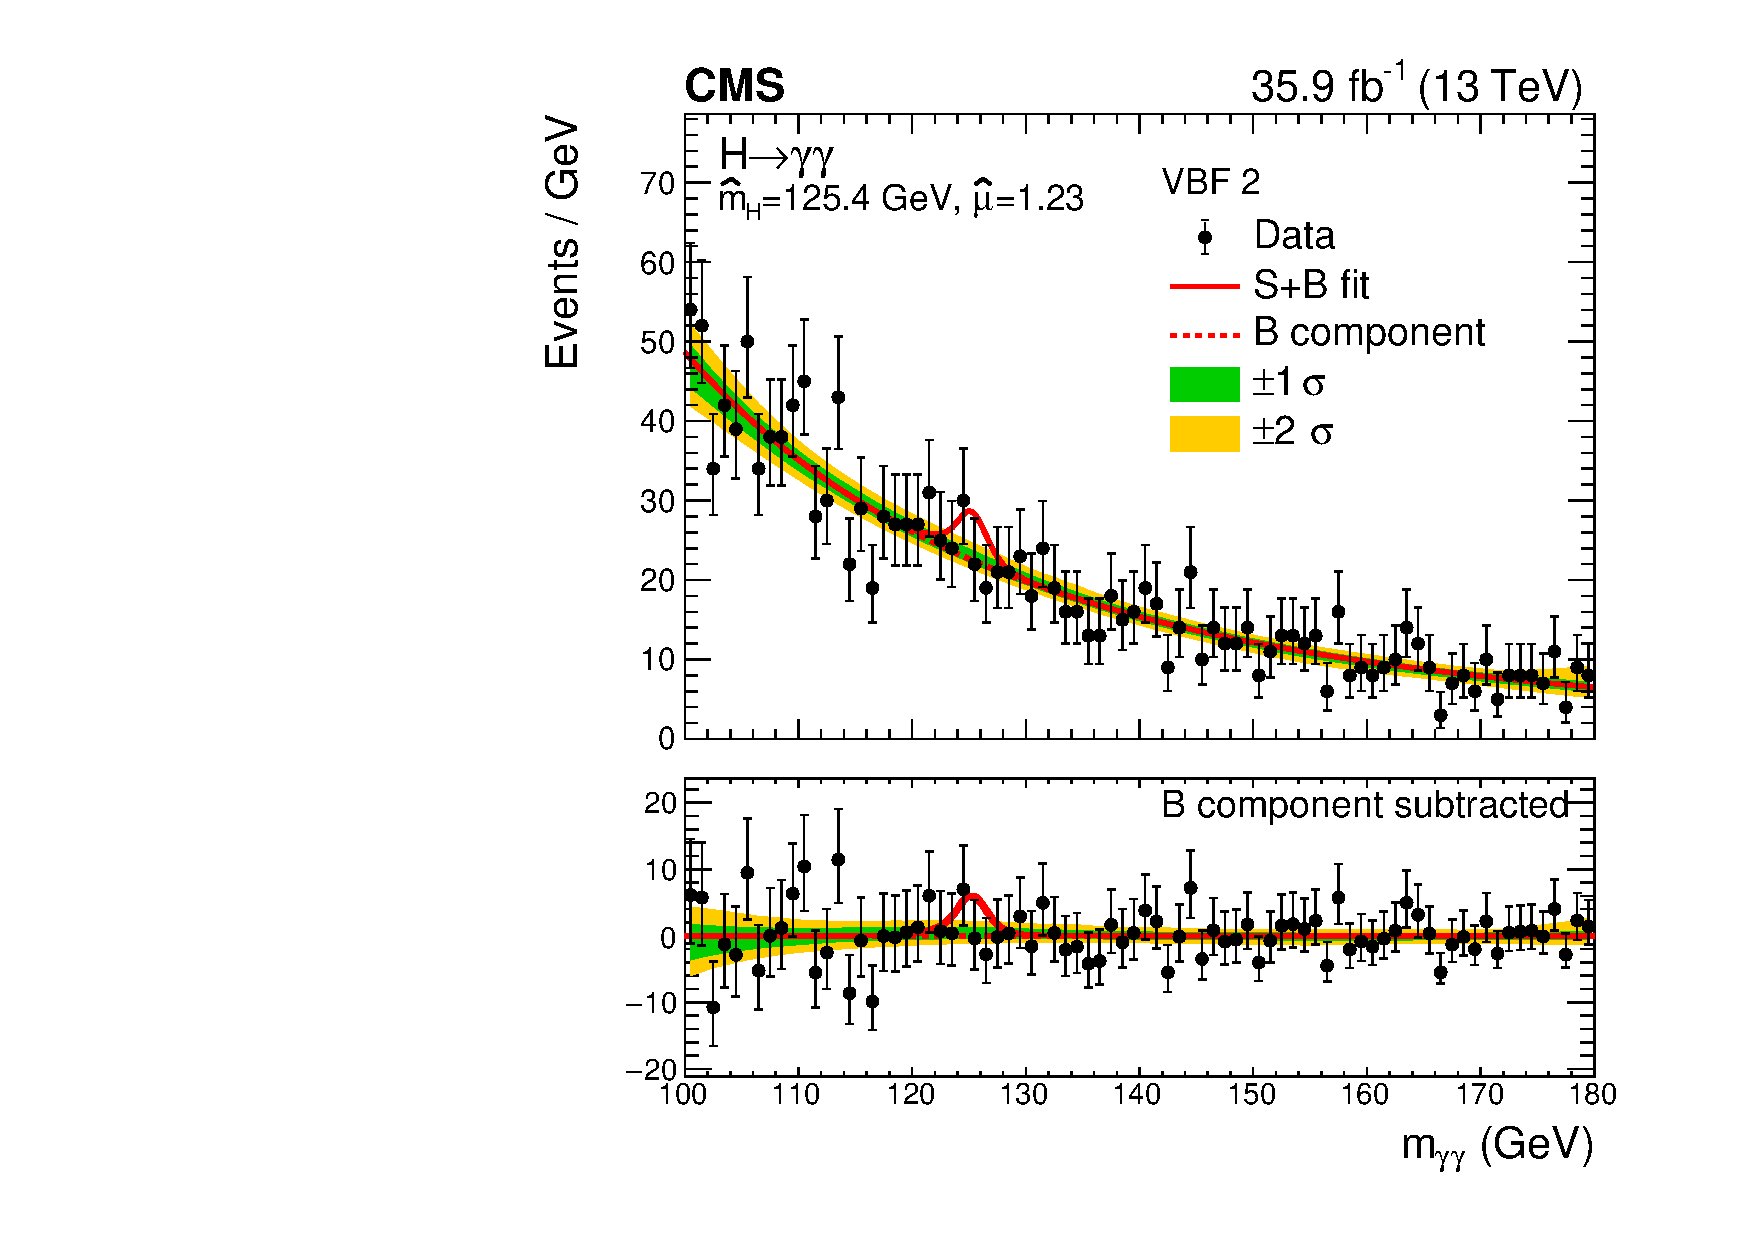
\includegraphics[width=0.47\textwidth]{figures/stats_results/SBplots_jackWSnewVBFTag_2_13TeV.pdf}
    \end{center}
    \caption{VBF category mass fits for BDT-based VBF tag (left) and the DCNN-based VBF tag (right).
             Categories are shown in order from the most stringent to least: VBF 0 at the top to VBF 2 at the bottom.}
        \label{fig:stats_results:vbf_mass_plots}
\end{figure}


\begin{landscape}
    \begin{table}
        \centering
        \resizebox{1.5\textwidth}{!}{%
        \renewcommand{\arraystretch}{1.2}
        \begin{tabular}{rcccccccccccccc}
        \thickhline
            \multirow{2}{*}{Event categories} &\multicolumn{13}{c}{Expected SM 125\,GeV Higgs boson signal (BDT-based VBF tag)} & Bkg \\ \cline{2-14}
          &  Total & ggH & VBF & \ttH & bbH & tHq & tHW & WH lep & ZH lep & WH had & ZH had &   $\sigma_{\text{eff}}$  & $\sigma_{\text{HM}}$ & (GeV$^{-1}$) \\
          &  & & & & & & & & & & & (GeV) & (GeV) & \\
        \hline
        \rowcolor{GGH0} Untagged 0 &    32.5  &  72.0 \% &  16.6 \% &  2.6 \% &  0.6 \% &  0.7 \% &  0.3 \% &  0.6 \% &  0.3 \% &  4.2 \% &  2.2 \%& 1.32 & 1.26 & 21.8 \\
        \rowcolor{GGH1} Untagged 1 &    469.3  &  86.5 \% &  7.9 \% &  0.6 \% &  1.2 \% &  0.1 \% &  $<$0.05 \% &  0.5 \% &  0.3 \% &  1.9 \% &  1.1 \%& 1.46 & 1.32 & 925.1 \\
        \rowcolor{GGH2} Untagged 2 &    678.3  &  89.9 \% &  5.4 \% &  0.4 \% &  1.2 \% &  0.1 \% &  $<$0.05 \% &  0.5 \% &  0.3 \% &  1.4 \% &  0.8 \%& 1.93 & 1.67 & 2391.7 \\
        \rowcolor{GGH3} Untagged 3 &    624.3  &  91.3 \% &  4.4 \% &  0.5 \% &  1.0 \% &  0.1 \% &  $<$0.05 \% &  0.5 \% &  0.3 \% &  1.2 \% &  0.7 \%& 2.61 & 2.27 & 4855.1 \\
        \rowcolor{VBF0} VBF 0 &    9.3  &  15.5 \% &  83.2 \% &  0.4 \% &  0.4 \% &  0.3 \% &  $<$0.05 \% &  $<$0.05 \% &  $<$0.05 \% &  0.2 \% &  $<$0.05 \%& 1.52 & 1.31 & 1.6 \\
        \rowcolor{VBF1} VBF 1 &    8.0  &  28.4 \% &  69.7 \% &  0.4 \% &  0.6 \% &  0.4 \% &  $<$0.05 \% &  0.1 \% &  $<$0.05 \% &  0.3 \% &  0.1 \%& 1.66 & 1.38 & 3.3 \\
        \rowcolor{VBF2} VBF 2 &    25.2  &  45.1 \% &  51.2 \% &  0.9 \% &  0.8 \% &  0.6 \% &  0.1 \% &  0.2 \% &  0.1 \% &  0.8 \% &  0.3 \%& 1.64 & 1.37 & 18.9 \\
        \ttH Hadronic &    5.6  &  7.0 \% &  0.7 \% &  81.1 \% &  2.1 \% &  4.3 \% &  2.1 \% &  0.1 \% &  0.1 \% &  0.7 \% &  1.9 \%& 1.48 & 1.30 & 2.4 \\
        \ttH Leptonic &    3.8  &  1.5 \% &  $<$0.05 \% &  87.8 \% &  0.1 \% &  4.7 \% &  3.1 \% &  1.5 \% &  1.2 \% &  $<$0.05 \% &  $<$0.05 \%& 1.60 & 1.35 & 1.5 \\
        ZH Leptonic &    0.5  &  $<$0.05 \% &  $<$0.05 \% &  2.6 \% &  $<$0.05 \% &  $<$0.05 \% &  0.1 \% &  $<$0.05 \% &  97.3 \% &  $<$0.05 \% &  $<$0.05 \%& 1.65 & 1.43 & 0.1 \\
        WH Leptonic &    3.6  &  1.3 \% &  0.6 \% &  5.2 \% &  0.2 \% &  3.0 \% &  0.7 \% &  84.5 \% &  4.3 \% &  0.1 \% &  0.1 \%& 1.64 & 1.43 & 2.1 \\
        VH LeptonicLoose &    2.7  &  8.1 \% &  2.7 \% &  2.4 \% &  0.6 \% &  1.8 \% &  0.1 \% &  64.4 \% &  19.1 \% &  0.6 \% &  0.2 \%& 1.67 & 1.56 & 3.5 \\
        \rowcolor{VHH} VH Hadronic &    7.9  &  47.6 \% &  4.5 \% &  4.4 \% &  0.4 \% &  1.7 \% &  0.3 \% &  0.2 \% &  0.5 \% &  25.2 \% &  15.1 \%& 1.38 & 1.30 & 7.2 \\
        \rowcolor{VHM} VH MET &    4.0  &  18.7 \% &  2.6 \% &  15.4 \% &  0.4 \% &  2.1 \% &  1.2 \% &  26.8 \% &  30.4 \% &  1.4 \% &  0.9 \%& 1.56 & 1.39 & 3.5 \\
        \rowcolor{Gray} Total &    1875.0  &  86.9 \% &  7.1 \% &  1.0 \% &  1.1 \% &  0.2 \% &  $<$0.05 \% &  0.8 \% &  0.4 \% &  1.6 \% &  0.9 \%& 1.96 & 1.62 & 8237.8 \\
        \hline
            \multirow{2}{*}{} &\multicolumn{13}{c}{Expected SM 125\,GeV Higgs boson signal (DCNN-based VBF tag and Downstream Tags)} & \\ \cline{2-14}
        \hline
        \rowcolor{GGH0} Untagged 0 &    33.3  &  73.5 \% &  14.7 \% &  2.9 \% &  0.6 \% &  0.7 \% &  0.3 \% &  0.6 \% &  0.3 \% &  4.2 \% &  2.2 \%& 1.26 & 1.19 &  21.7 \\
        \rowcolor{GGH1} Untagged 1 &    466.5  &  87.2 \% &  7.3 \% &  0.6 \% &  1.2 \% &  0.1 \% &  $<$0.05 \% &  0.5 \% &  0.3 \% &  1.8 \% &  1.1 \%& 1.46 & 1.31 &  910.0 \\
        \rowcolor{GGH2} Untagged 2 &    674.8  &  90.3 \% &  5.0 \% &  0.4 \% &  1.2 \% &  0.1 \% &  $<$0.05 \% &  0.5 \% &  0.3 \% &  1.4 \% &  0.8 \%& 1.92 & 1.64 &  2415.6 \\
        \rowcolor{GGH3} Untagged 3 &    620.5  &  91.6 \% &  4.1 \% &  0.5 \% &  1.0 \% &  0.1 \% &  $<$0.05 \% &  0.5 \% &  0.3 \% &  1.2 \% &  0.7 \%& 2.62 & 2.29 &  4848.2 \\
        \rowcolor{VBF0} VBF 0 &    14.2  &  9.5 \% &  89.7 \% &  0.2 \% &  0.3 \% &  0.2 \% &  $<$0.05 \% &  0.1 \% &  $<$0.05 \% &  0.1 \% &  $<$0.05 \%& 1.70 & 1.41 &  3.4 \\
        \rowcolor{VBF1} VBF 1 &    17.2  &  25.0 \% &  73.2 \% &  0.3 \% &  0.5 \% &  0.4 \% &  $<$0.05 \% &  0.1 \% &  $<$0.05 \% &  0.3 \% &  0.1 \%& 1.78 & 1.43 & 10.6 \\
        \rowcolor{VBF2} VBF 2 &    19.6  &  44.2 \% &  51.7 \% &  0.7 \% &  0.9 \% &  0.6 \% &  $<$0.05 \% &  0.2 \% &  $<$0.05 \% &  1.2 \% &  0.5 \%& 1.78 & 1.40 & 23.0 \\
        \rowcolor{VHH} VH Hadronic &    7.9  &  47.3 \% &  4.5 \% &  4.8 \% &  0.4 \% &  1.7 \% &  0.3 \% &  0.3 \% &  0.5 \% &  25.2 \% &  14.9 \%& 1.46 & 1.38 & 7.2 \\
        \rowcolor{VHM} VH MET &    3.9  &  19.0 \% &  3.0 \% &  13.4 \% &  0.5 \% &  2.2 \% &  1.2 \% &  27.3 \% &  30.9 \% &  1.5 \% &  1.0 \%& 1.61 & 1.46 & 3.4 \\
        \rowcolor{Gray} Total &    1874.3  &  86.9 \% &  7.1 \% &  1.0 \% &  1.1 \% &  0.1 \% &  $<$0.05 \% &  0.8 \% &  0.4 \% &  1.6 \% &  0.9 \%& 1.96 & 1.61 & 8252.9 \\
        \thickhline
        \end{tabular}%
    }
        \caption{Expected signal yields per category for BDT-based VBF tag (top) and DCNN-based VBF tag (bottom). 
                 Only the downstream tags are shown for the DCNN-based tag as the others are unaffected.
                 The width values $\sigma_{\text{eff}}$ and $\sigma_{\text{HM}}$ correspond to the smallest interval 
                 containing 68.3\% of the \mgg distribution and the width at half maximum of the signal peak respectively.}
        \label{tab:stats_results:yield_table}
    \end{table}
\end{landscape}
\begin{table}[h!]
    \centering
    \renewcommand{\arraystretch}{1.3}
    \begin{tabular}{r|cccc}
        \thickhline
        & \multicolumn{4}{c}{$S/\sqrt{S+B}$} \\ 
        VBF tag & VBF 0 & VBF 1 & VBF 2 & Total \\
        \hline
        BDT-based  & 2.02 & 1.25 & 1.35 & 2.73\\
        DCNN-based & 2.44 & 1.65 & 0.97 & 3.10\\
        \thickhline
    \end{tabular}
    \caption{VBF tag category expected signal significances comparing BDT-based VBF tag to the DCNN-based VBF tag.}
    \label{tab:stats_results:sig_table}
\end{table}



The final combined mass plots weighted by sensitivity and unweighted are shown in Figure \ref{fig:stats_results:comb_mass_plots}. The change to a DCNN-based VBF tag does not have a significant effect on these plots.
\begin{figure}[h!]
    \begin{center}
        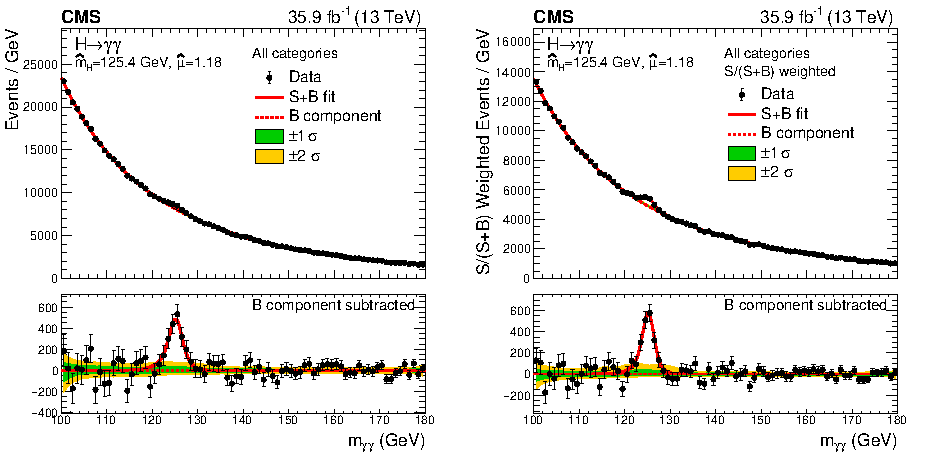
\includegraphics[width=1.0\textwidth]{figures/stats_results/CMS-HIG-16-040_Figure_014.pdf}
    \end{center}
    \caption{Diphoton mass distribution plots for all categories combined using the BDT-based VBF tag.}
        \label{fig:stats_results:comb_mass_plots}
\end{figure}








\subsection{Signal Strength Likelihood Scans}
General prescription of likelihood scans
The test statistic used is the twice-negative delta log-likelihood ($2\Delta{\mathrm{NLL}}$), 
\begin{equation}
    2\Delta{\mathrm{NLL}} = -2\ln{\mathcal{L}}(\mu,\hat{m}_{H,\mu},\vec{n}_{\mu} | m_{\gamma\gamma}) + 2\ln\mathcal{L}(\hat{\mu},\hat{m}_{H},\hat{n} | m_{\gamma\gamma}),
\end{equation}
where $\hat{\mu}$, $\hat{m}_{H}$ and $\hat{n}$ are the best fit values for the signal strength modifier, Higgs mass and nuisance parameters respectively. 
The parameters $\mu$, $\hat{m}_{H,\mu}$ and $\vec{n}_{\mu}$ are the global signal strength being profiled in the likelihood scan, the Higgs mass allowed to float for a given value of $\mu$, and the nuisance parameter values also allowed to float. 

This procedure is used to measure the global $\mu$, the production mode $\mu$s and the fermionic vs bosonic production $\mu$s. 

\subsubsection{Global Signal Strength Likelihood Scan}
To calculate the uncertainty associated with the measurement of the global signal strength a likelihood scan is performed with a test statistic and profiling in the value of $\mu$.
The contribution of statistical uncertainty is determined by performing the likelihood scan with the nuisance parameters associated with systematic uncertainties removed. 
The systematic contribution is then the difference in quadrature between these values and the total uncertainty from the full fit. 
The $2\Delta{\mathrm{NLL}}$ values of the global $\mu$ likelihood scans are shown in Figure \ref{fig:stats_results:global_mu_scan}.
\begin{figure}[h!]
    \begin{center}
        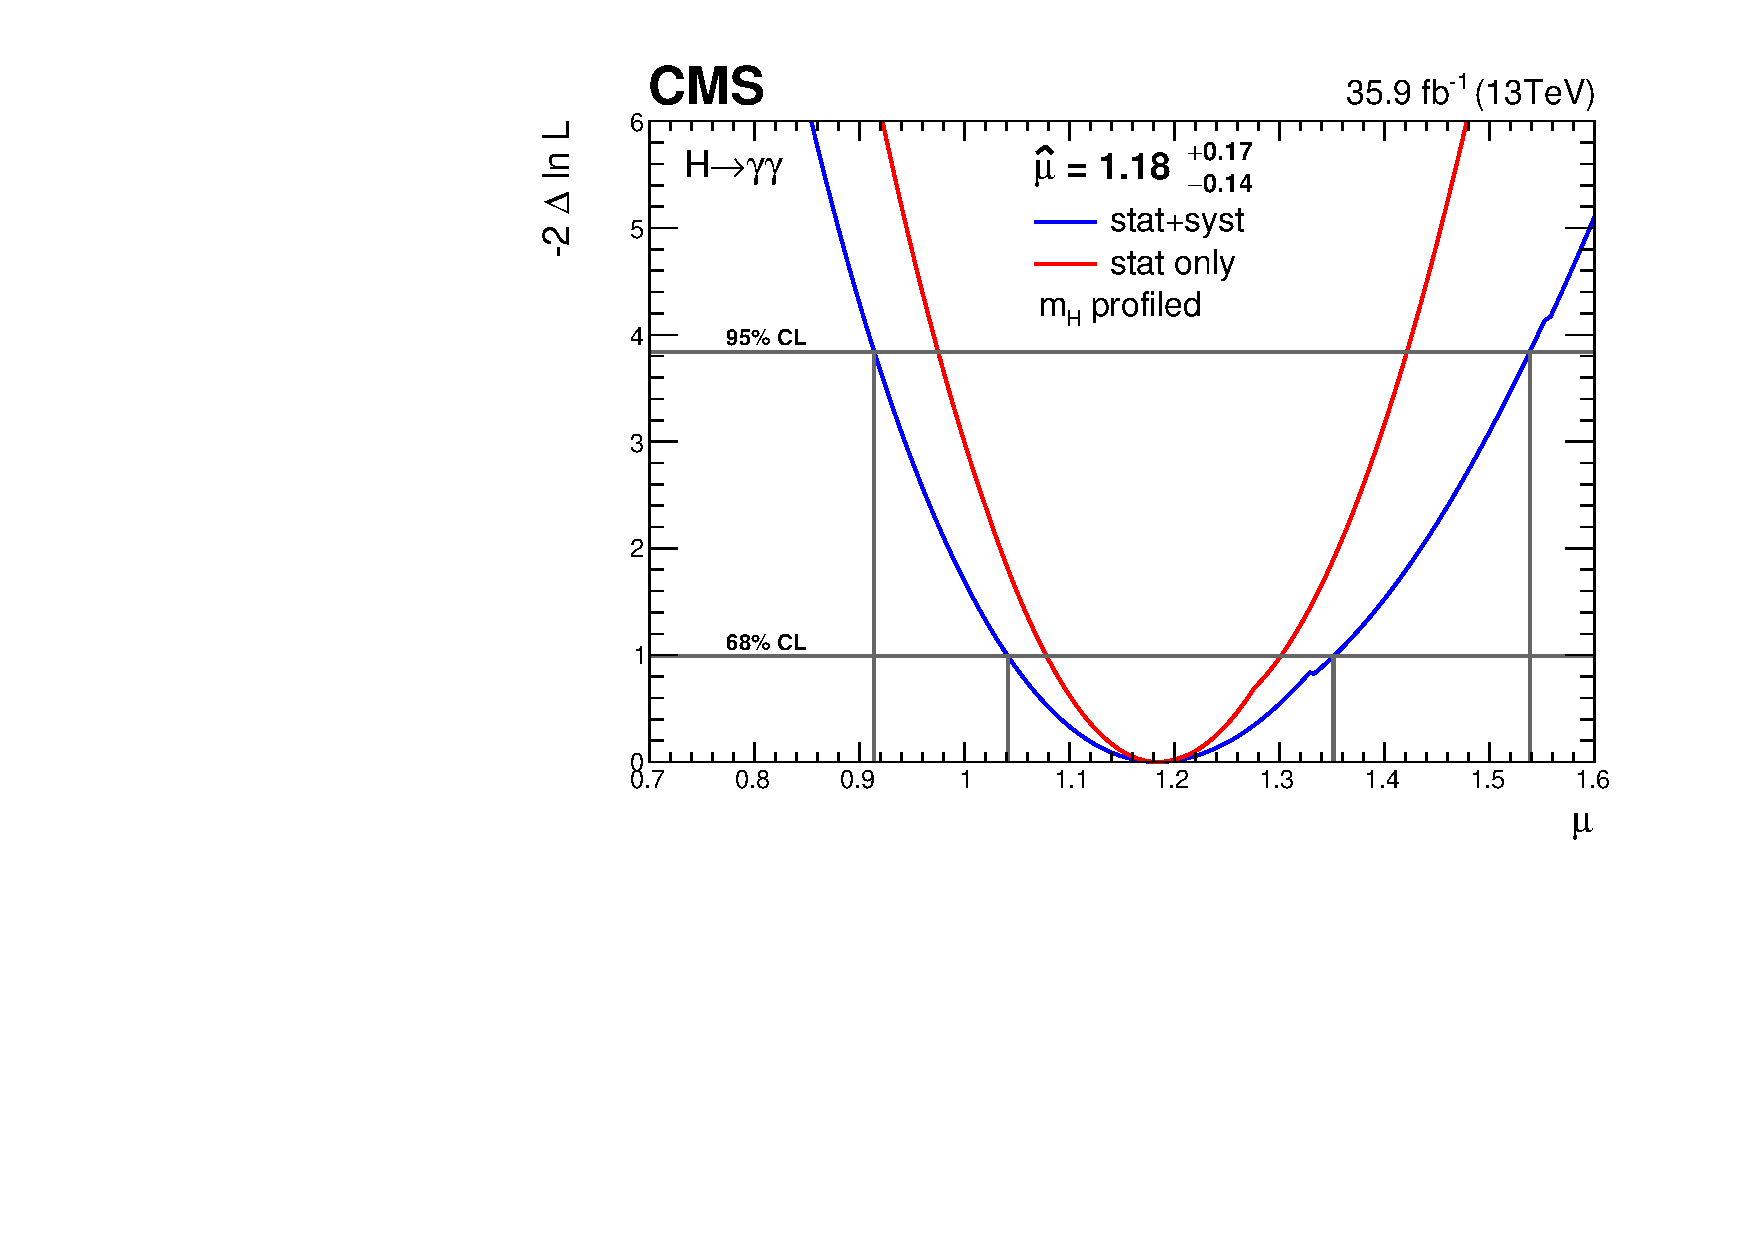
\includegraphics[width=0.6\textwidth]{figures/stats_results/CMS-HIG-16-040_Figure_016.pdf}
        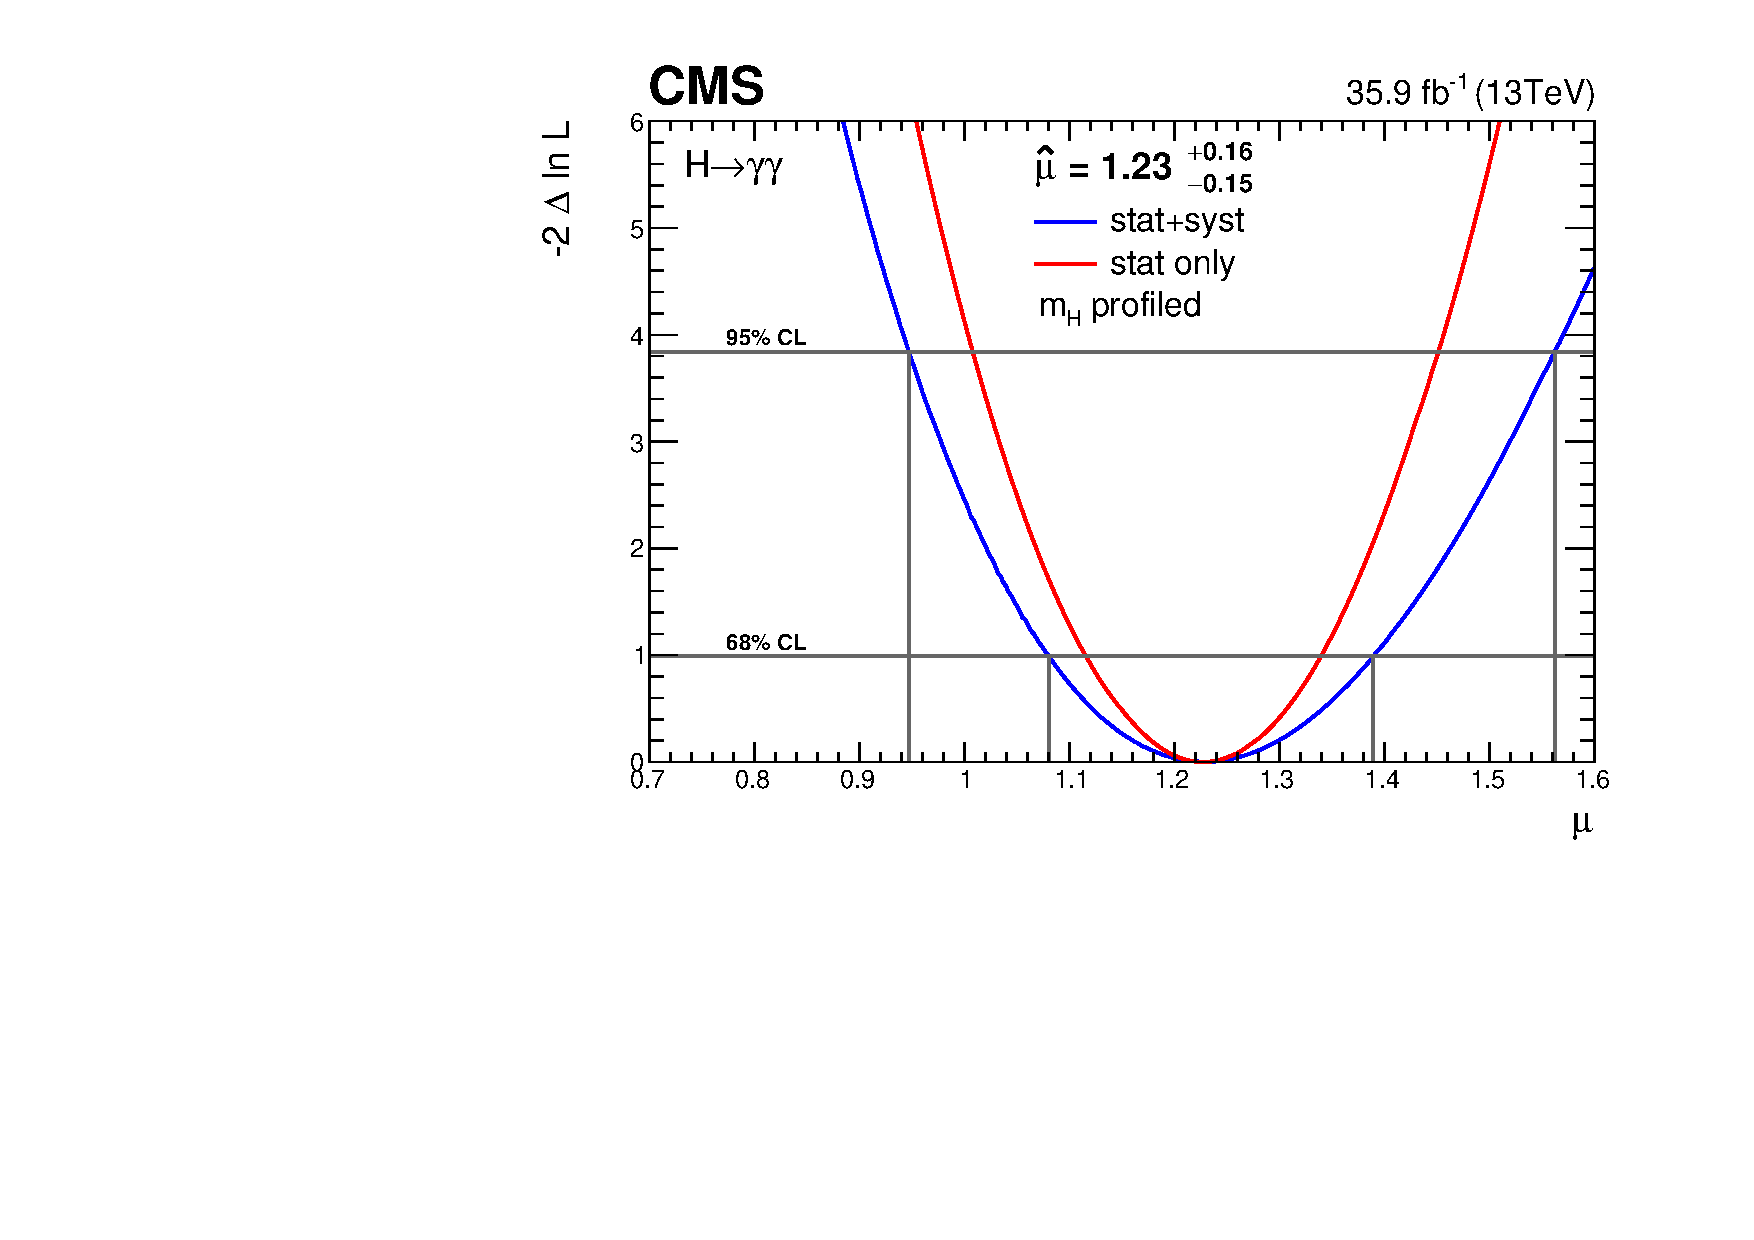
\includegraphics[width=0.6\textwidth]{figures/stats_results/MuScanProfileMH.pdf}
    \end{center}
    \caption{Likelihood scan of the global signal strength modifier $\mu$ with a $2\Delta{\mathrm{NLL}}$ test statistic for analysis with BDT-based VBF tag (left) and DCNN-based VBF tag (right).}
        \label{fig:stats_results:global_mu_scan}
\end{figure}

The measured value for $\mu$ and its associated uncertainties in the BDT-based case are found to be $\hat{\mu} = 1.18^{+0.17}_{-0.14} = 1.18^{+0.12}_{-0.11}(\mathrm{stat.})^{+0.09}_{-0.07}(\mathrm{syst.})^{+0.07}_{-0.06}(\mathrm{theo.})$.
The best fit value for the Higgs boson mass is found to be $\hat{m}_{H}=125.4\pm{0.3}=125.4\pm{0.2}(\mathrm{stat}.)\pm{0.2}(\mathrm{syst}.)$. 
A precise determination of the systematic effects on the mass value and therefore a precise determination of the mass itself are beyond the scope of this thesis.

The measured value for $\mu$ is found to be larger in the DCNN case with similar sized uncertainties: $\hat{\mu} = 1.23^{+0.16}_{-0.15} = 1.23^{+0.xx}_{-0.xx}(\mathrm{stat.})^{+0.xx}_{-0.xx}(\mathrm{syst.})^{+0.xx}_{-0.xx}(\mathrm{theo.})$.
The best fit value for the Higgs boson mass is unchanged. 














\subsubsection{Production Mode Signal Strength Modifiers}
Likelihood scans specific to each production mode are carried out in similar way to the global case, but with some differences. 
Instead of a single global $\mu$ and likelihood scan there are four, one for each production mode. 
For each case the corresponding $\mu$ is profiled and the others are allowed to float in the fit. 
The results of these likelihood scans are shown in Figure \ref{fig:stats_results:prod_mu_scans}. 
\begin{figure}[h!]
    \begin{center}
        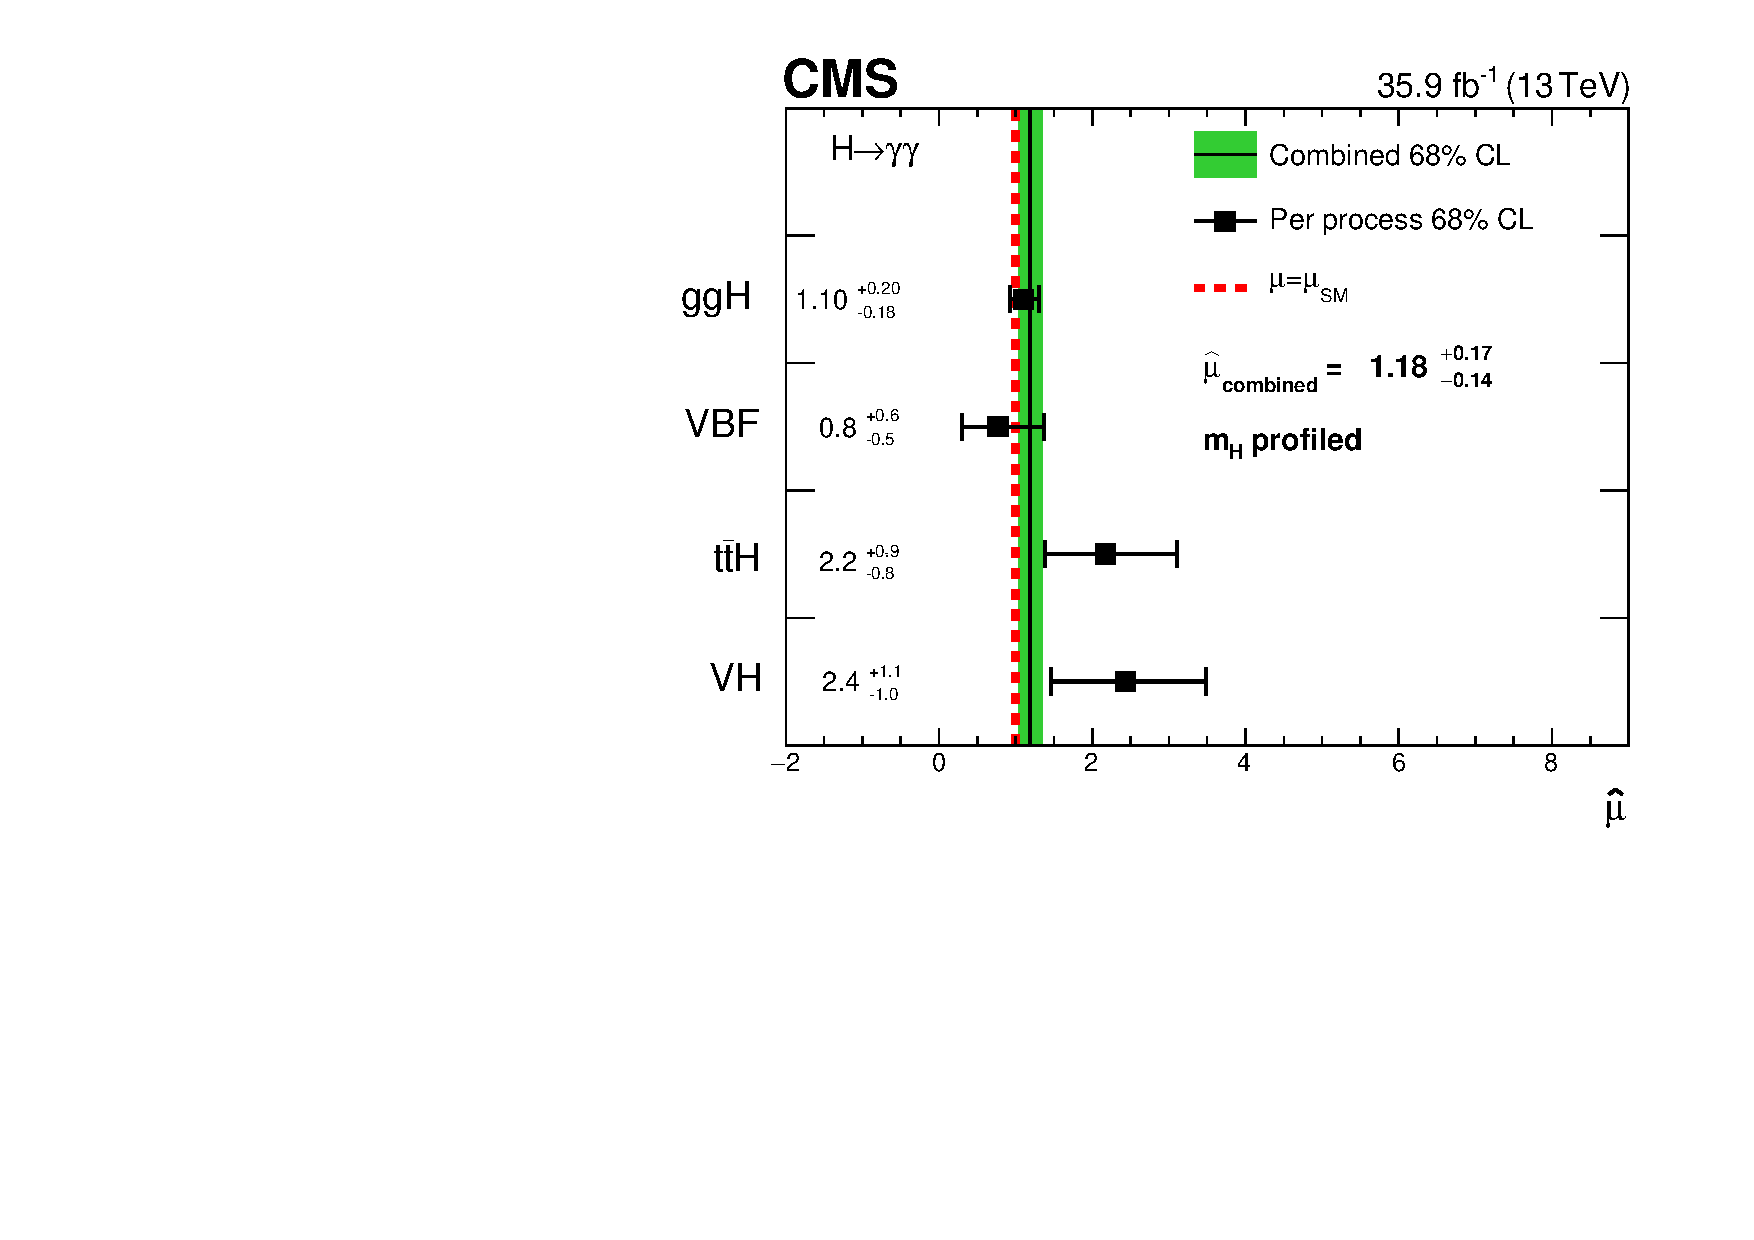
\includegraphics[width=0.75\textwidth]{figures/stats_results/CMS-HIG-16-040_Figure_017.pdf}
        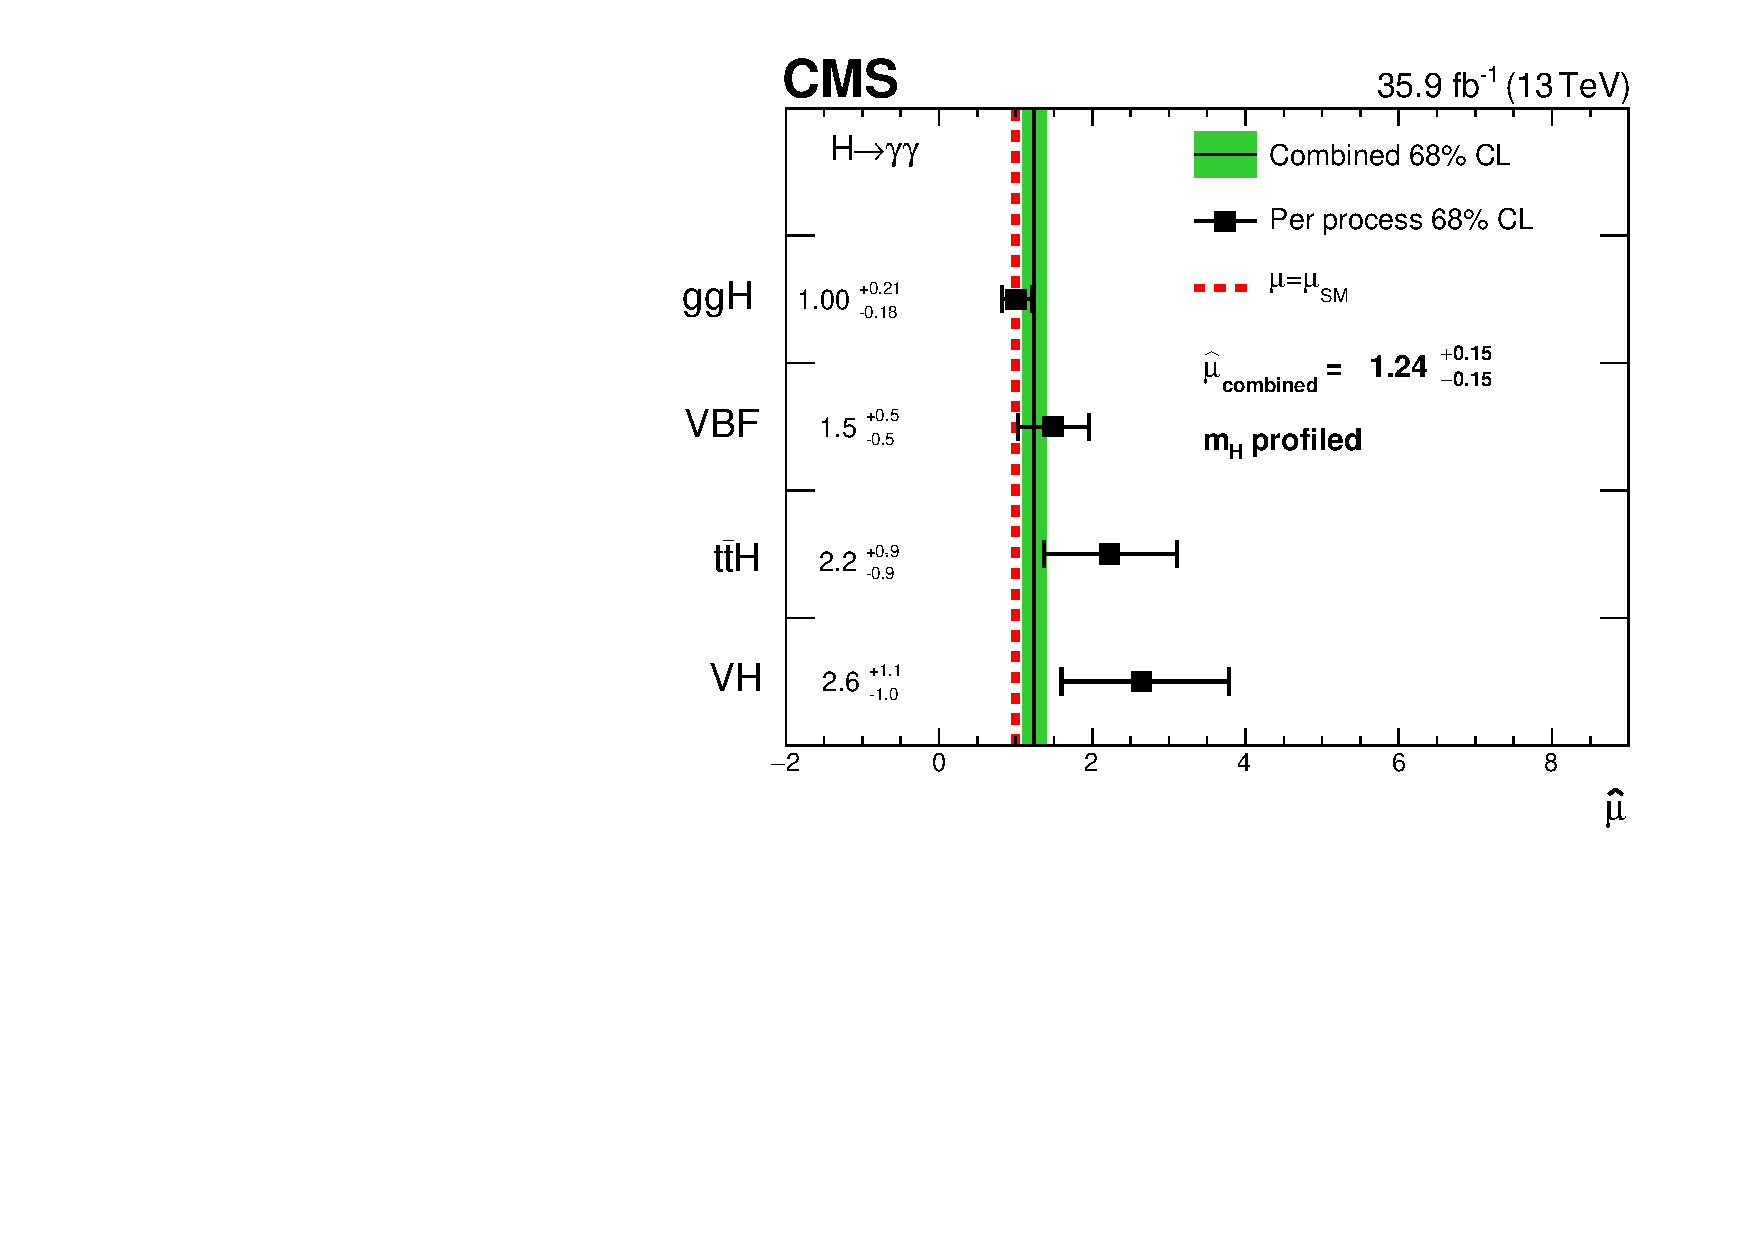
\includegraphics[width=0.75\textwidth]{figures/stats_results/PerProcessMuProfileMH.pdf}
    \end{center}
    \caption{Likelihood scan results of the production mode signal strength modifiers $\mu$ with a $2\Delta{\mathrm{NLL}}$ test statistic. Analysis with a BDT-based VBF tag is shown on the left and the DCNN-based variant is on the right.}
        \label{fig:stats_results:prod_mu_scans}
\end{figure}

The DCNN-based VBF tag leads to a change in the VBF measurement from $\mu_{\mathrm{VBF}}=0.8^{+0.6}_{-0.5}$ to $\mu_{\mathrm{VBF}}=1.5^{+0.5}_{-0.4}$.
The measured signal strength has increased, and there has been a reduction in the uncertainty of its measurement.
The other production modes are mostly unchanged except for the ggH and VH which correspond to tags downstream from VBF.


The same approach is used to extract the ratio of observed cross sections to the SM expectation as part of the simplified template cross section (STXS) framework Stage 0 \cite{LHCHXS}.
This scheme is aimed at reducing the impact of theory uncertainties due to extrapolation to the full phase space from the fiducial region of the analysis. 
This imposes a criterion on the Higgs boson rapidity of $y<2.5$ and splits the VH into separate WH, ZH and VH Hadronic categories. 
The results of measuring these ratios are shown in Figure \ref{fig:stats_results:stxs}.
\begin{figure}[h!]
    \begin{center}
        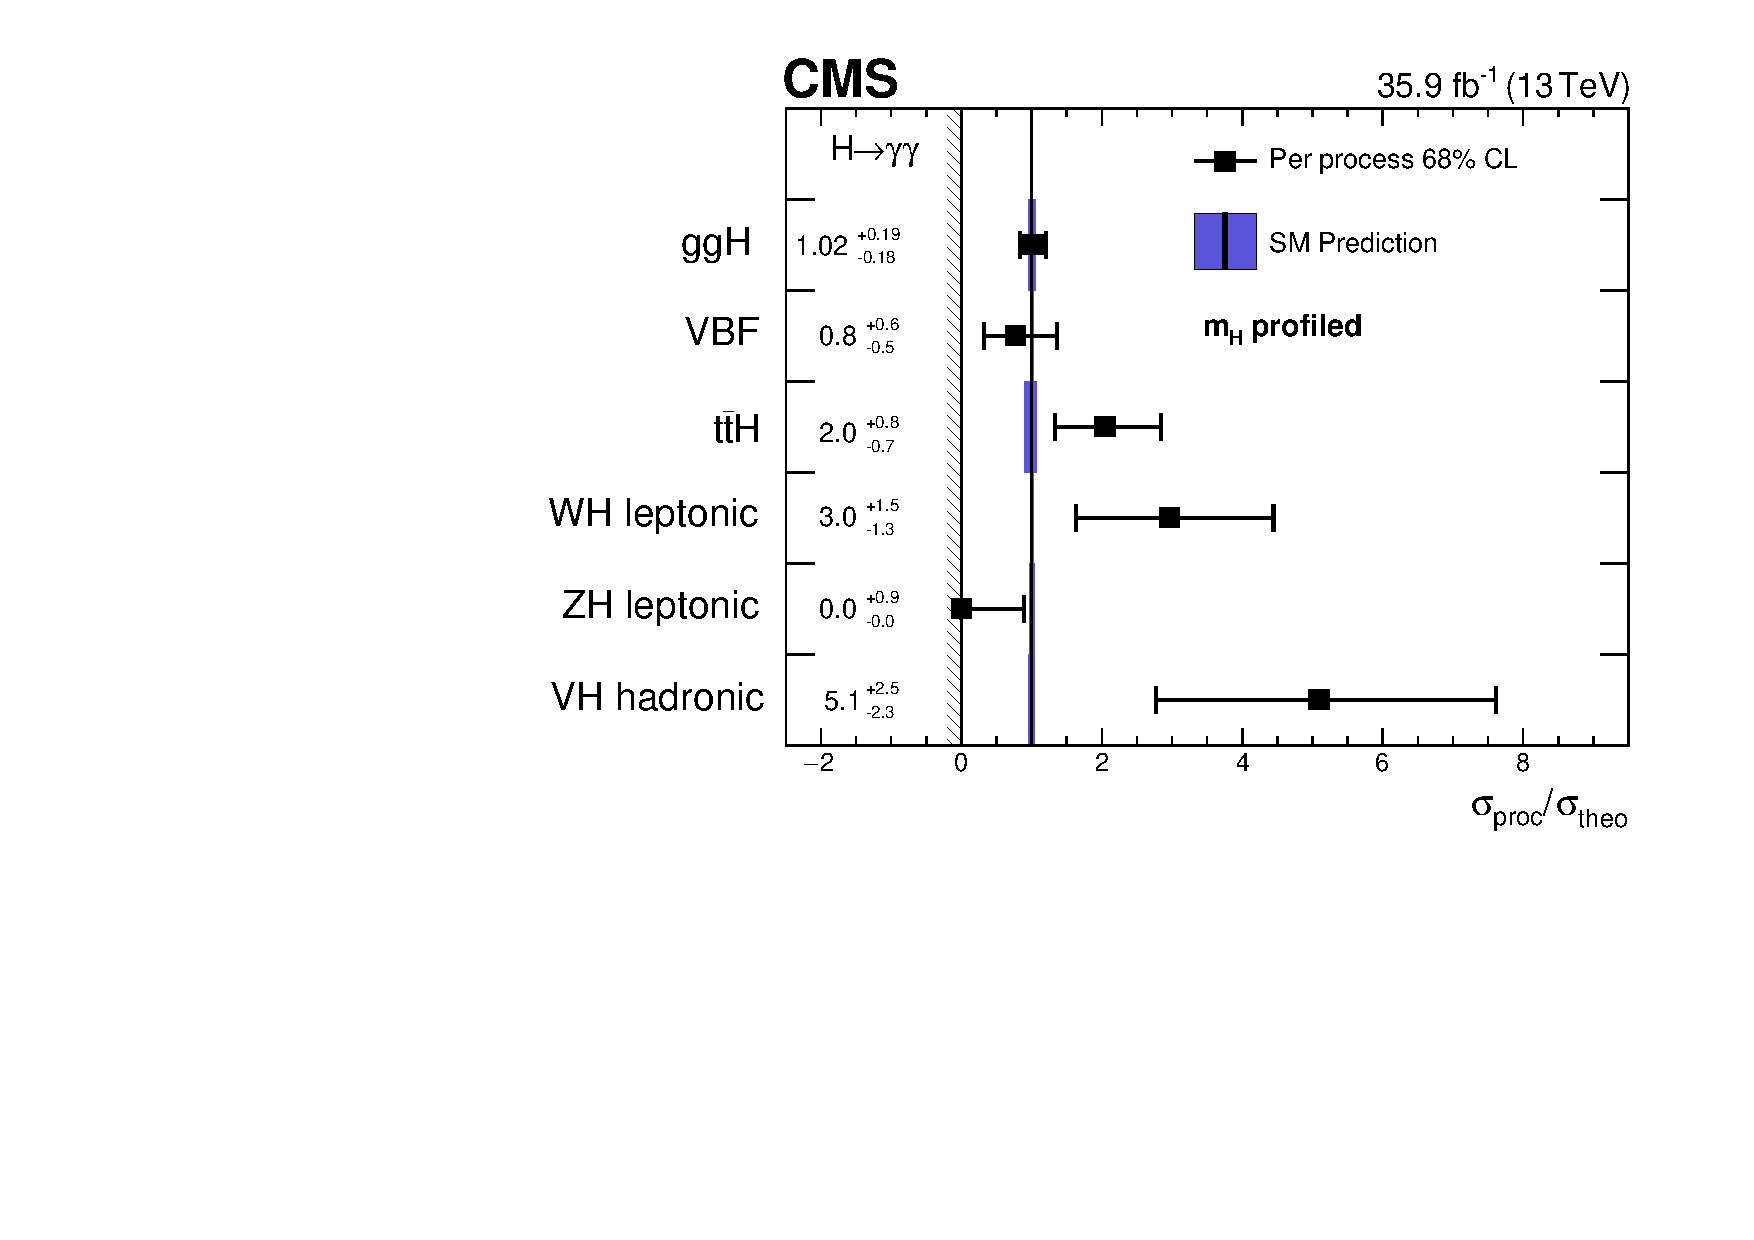
\includegraphics[width=0.75\textwidth]{figures/stats_results/CMS-HIG-16-040_Figure_018.pdf}
        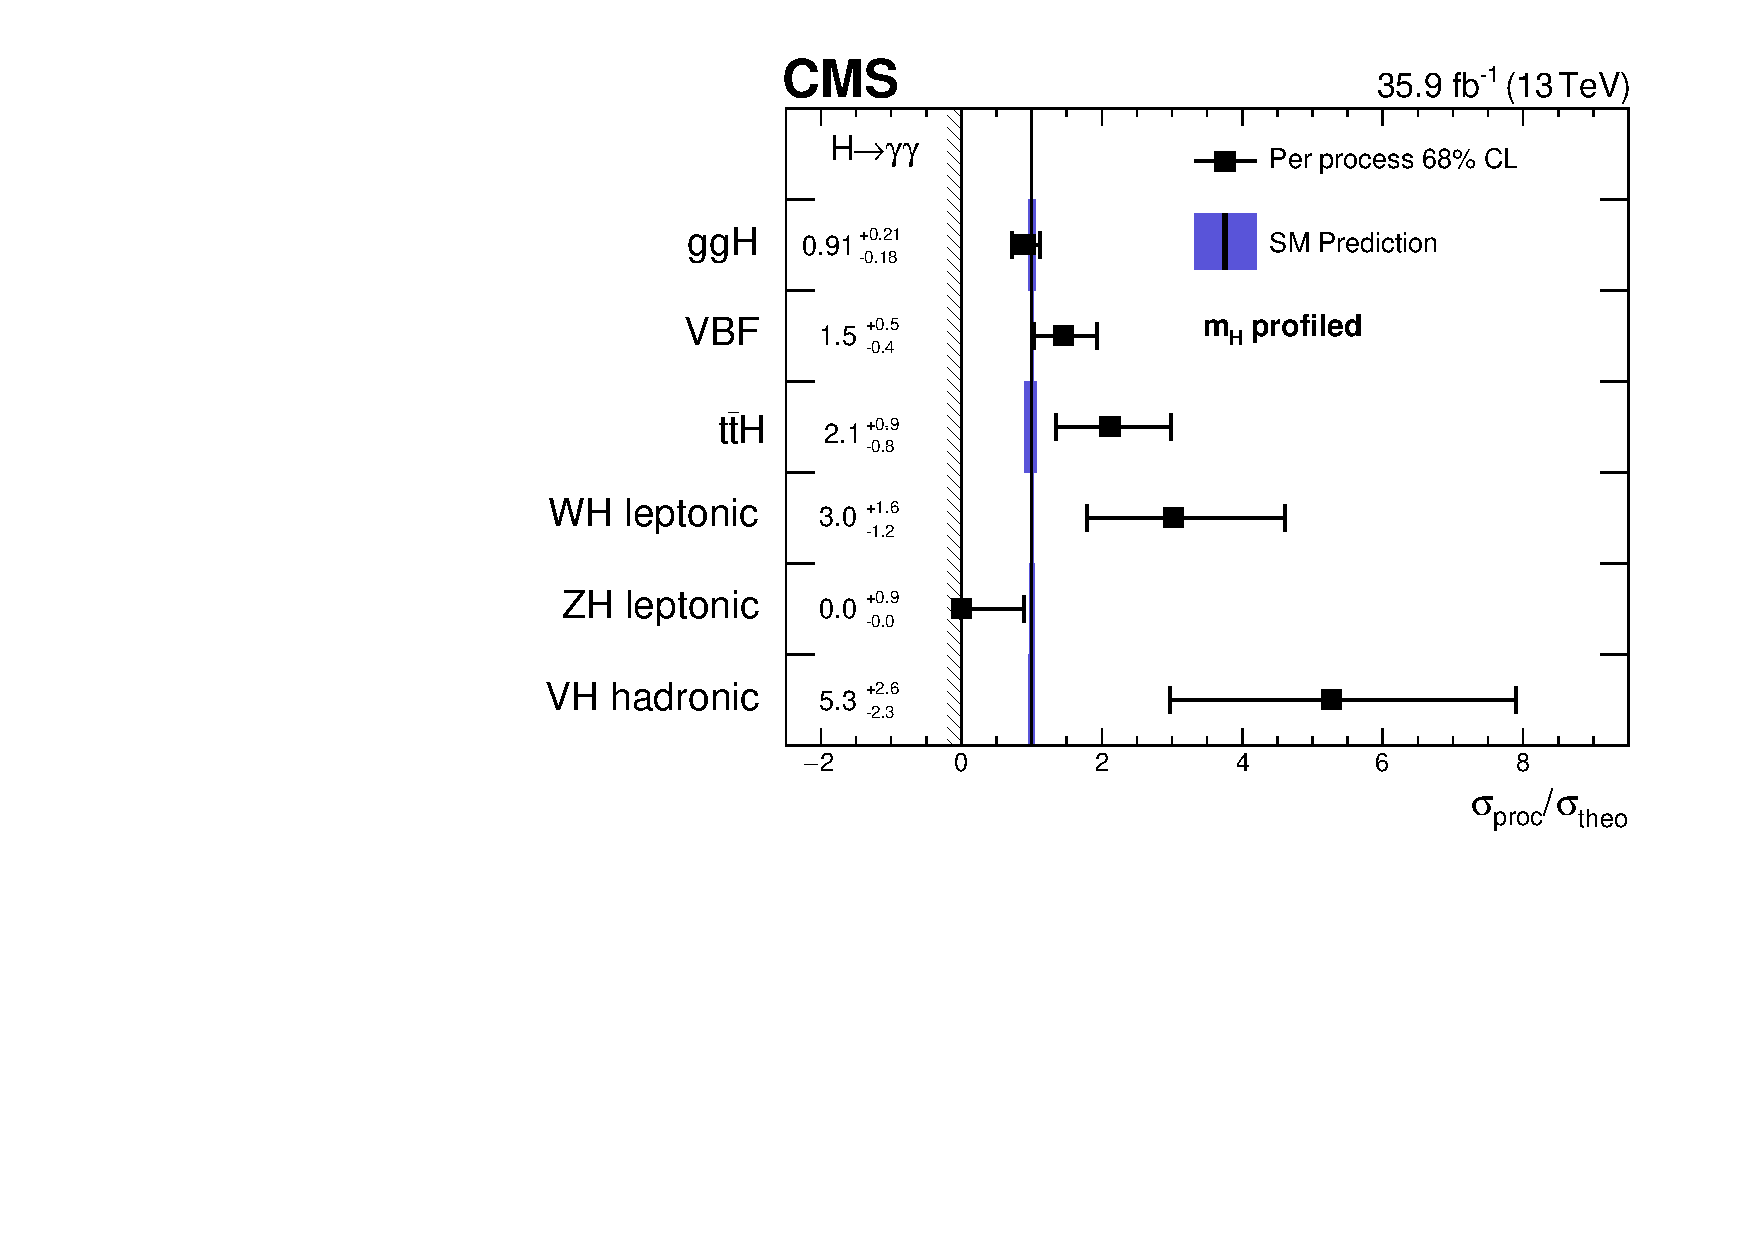
\includegraphics[width=0.75\textwidth]{figures/stats_results/STXSPerProcessMuProfileMH.pdf}
    \end{center}
    \caption{SM prediction to measured cross section ratios in the STXS Stage 0 framework. Analysis with a BDT-based VBF tag is shown on the left and the DCNN-based variant is on the right.}
        \label{fig:stats_results:stxs}
\end{figure}

The DCNN-based VBF tag has a similar effect in this scheme to the the production mode signal strengths. 
(The difference in the VH may be down to VH hadronic. Need to wait for the fix)






\subsubsection{Fermionic Versus Bosonic Production}
A measurement of the fermionic versus bosonic signal strength is performed with a 2D likelihood scan.
The procedure is similar to the above but with a signal strength for the bosonic production modes $\mu_{\mathrm{VBF},\mathrm{VH}}$ and the fermionic modes $\mu_{\mathrm{ggH},\mathrm{t\bar{t}H}}$.
A best fit point is found and then a $2\Delta\mathrm{NLL}$ test statistic is evaluated over a 2D space corresponding to different values of the two signal strength modifiers. 
The result with 68\% and 95\% confidence intervals is shown in Figure \ref{fig:stats_results:fermionic_bosonic}. 
\begin{figure}[h!]
    \begin{center}
        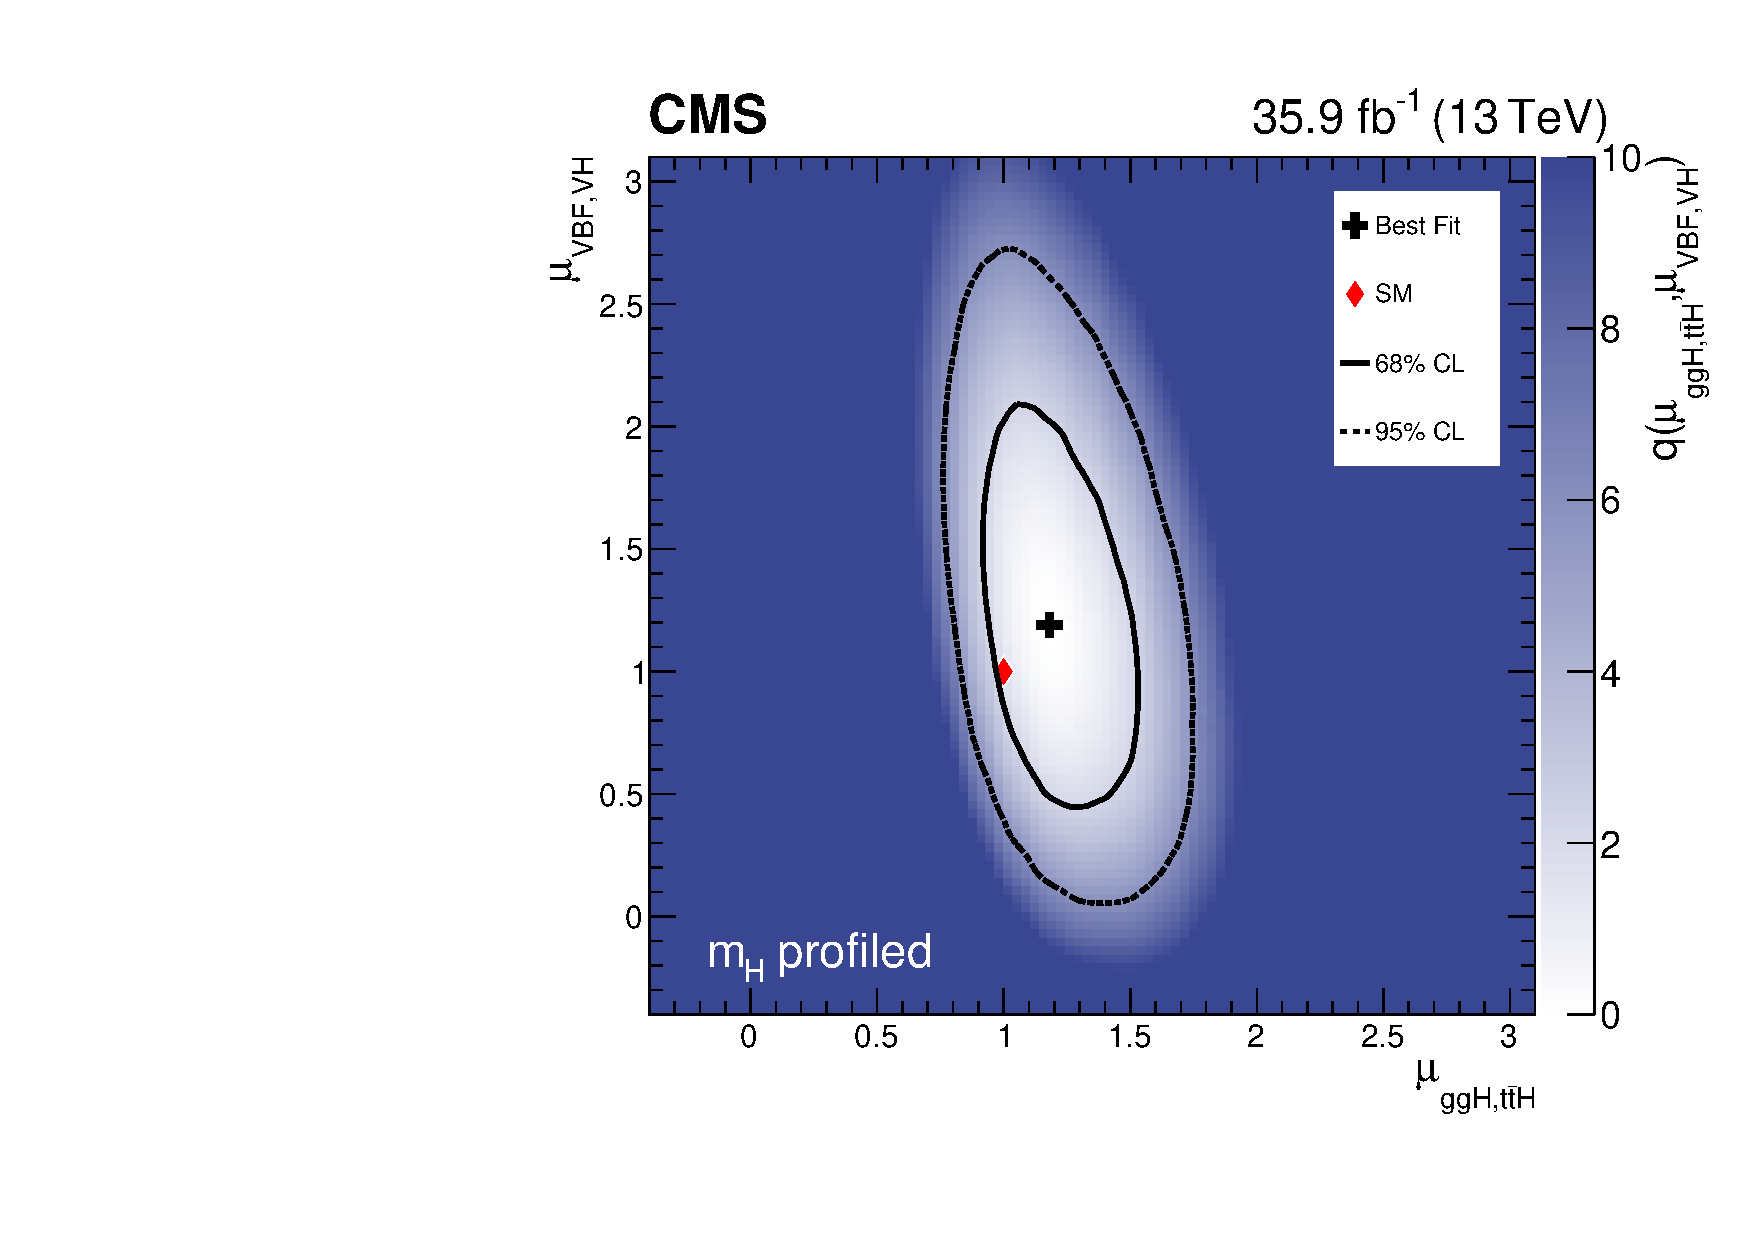
\includegraphics[width=0.49\textwidth]{figures/stats_results/CMS-HIG-16-040_Figure_019.pdf}
        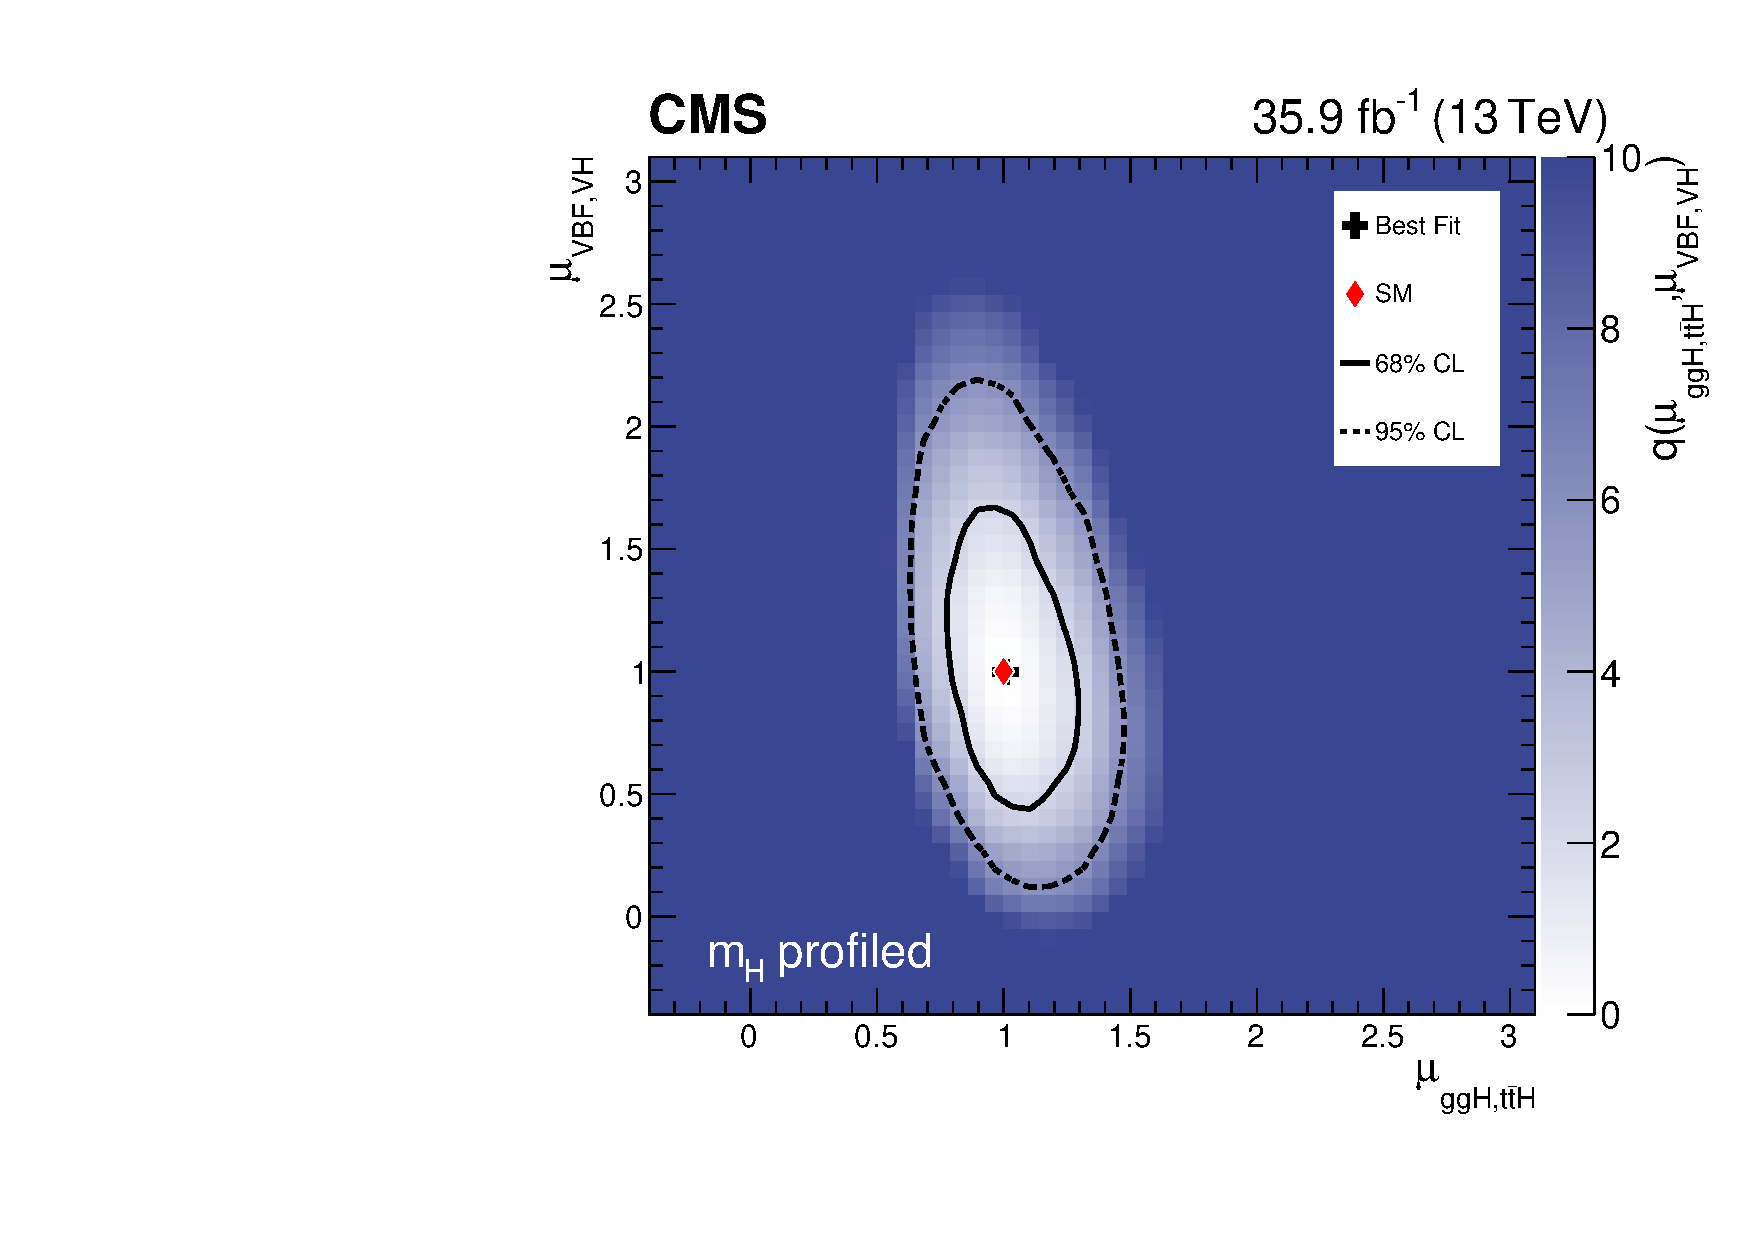
\includegraphics[width=0.49\textwidth]{figures/stats_results/RVRFScanProfileMH_col.pdf}
    \end{center}
    \caption{Two-dimensional likelihood scan of signal strength modifiers for bosonic (VBF, VH) and fermionic (ggH, \ttH) production modes. Analysis with a BDT-based VBF tag is shown on the left and the DCNN-based variant is on the right.}
        \label{fig:stats_results:fermionic_bosonic}
\end{figure}

The best fit point for the BDT-based case was found to be $\mu_{\mathrm{ggH},\mathrm{t\bar{t}H}} = 1.19^{+0.22}_{-0.18}$, $\mu_{\mathrm{VBF},\mathrm{VH}} = 1.21^{+0.58}_{-0.51}$.
The best fit point for the DCNN-based case was found to be $\mu_{\mathrm{ggH},\mathrm{t\bar{t}H}} = 1.xx^{+0.xx}_{-0.xx}$, $\mu_{\mathrm{VBF},\mathrm{VH}} = 1.xx^{+0.xx}_{-0.xx}$.
A significant reduction in the uncertainty of the bosonic production mode $\mu$ is observed along with an increase in its value.





\subsection{Couplings Measurements}
Deviation in the Higgs couplings from SM expectation are modelled within the $\kappa$ framework as described in \cite{Kappa}.
These differences are measured with two 2D likelihood scans: fermionic versus bosonic and photons versus gluons.
The $\kappa$ values not subject to the 2D likelihood scan are fixed at unity.
The resulting plots for the BDT-based and DCNN-based VBF tags are shown in Figure \ref{fig:stats_results:kappa}
\begin{figure}[h!]
    \begin{center}
        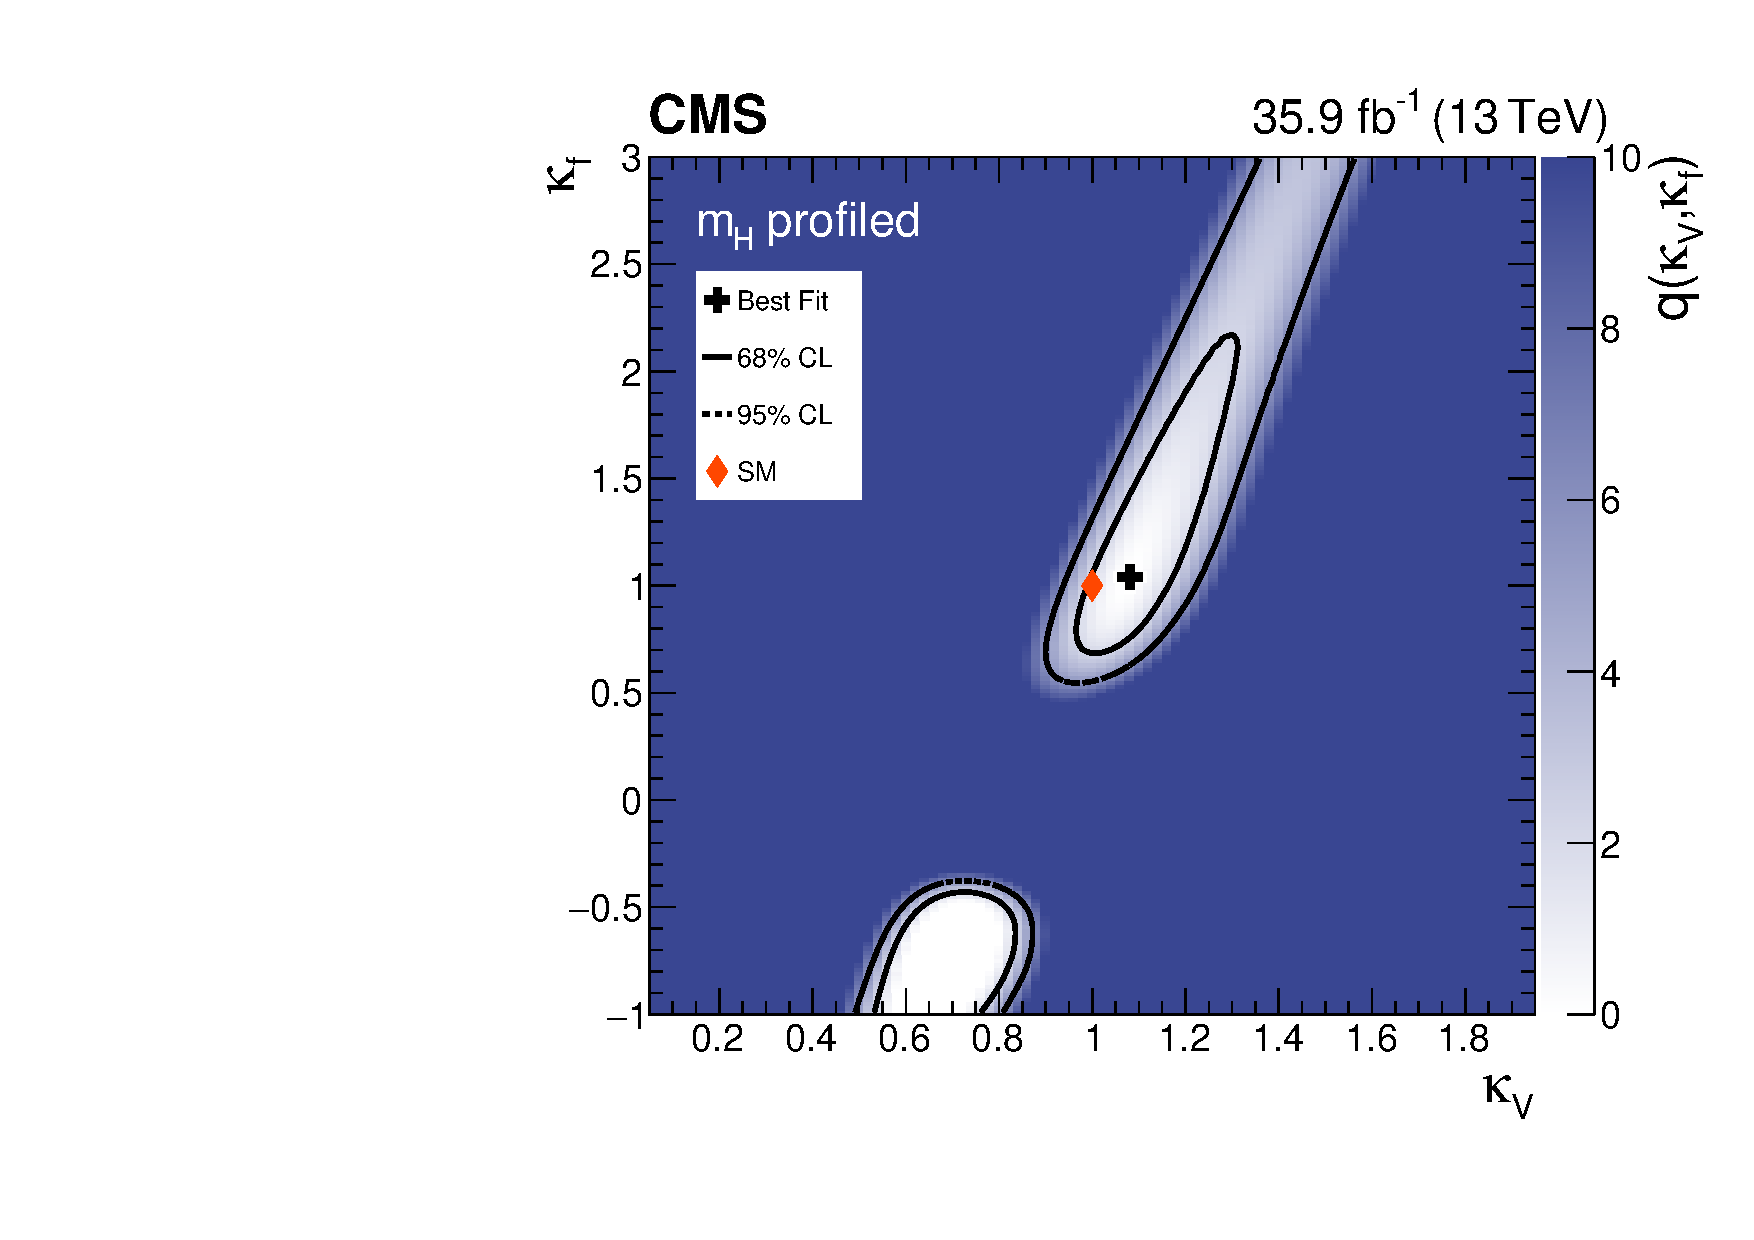
\includegraphics[width=0.49\textwidth]{figures/stats_results/CMS-HIG-16-040_Figure_020-a.pdf}
        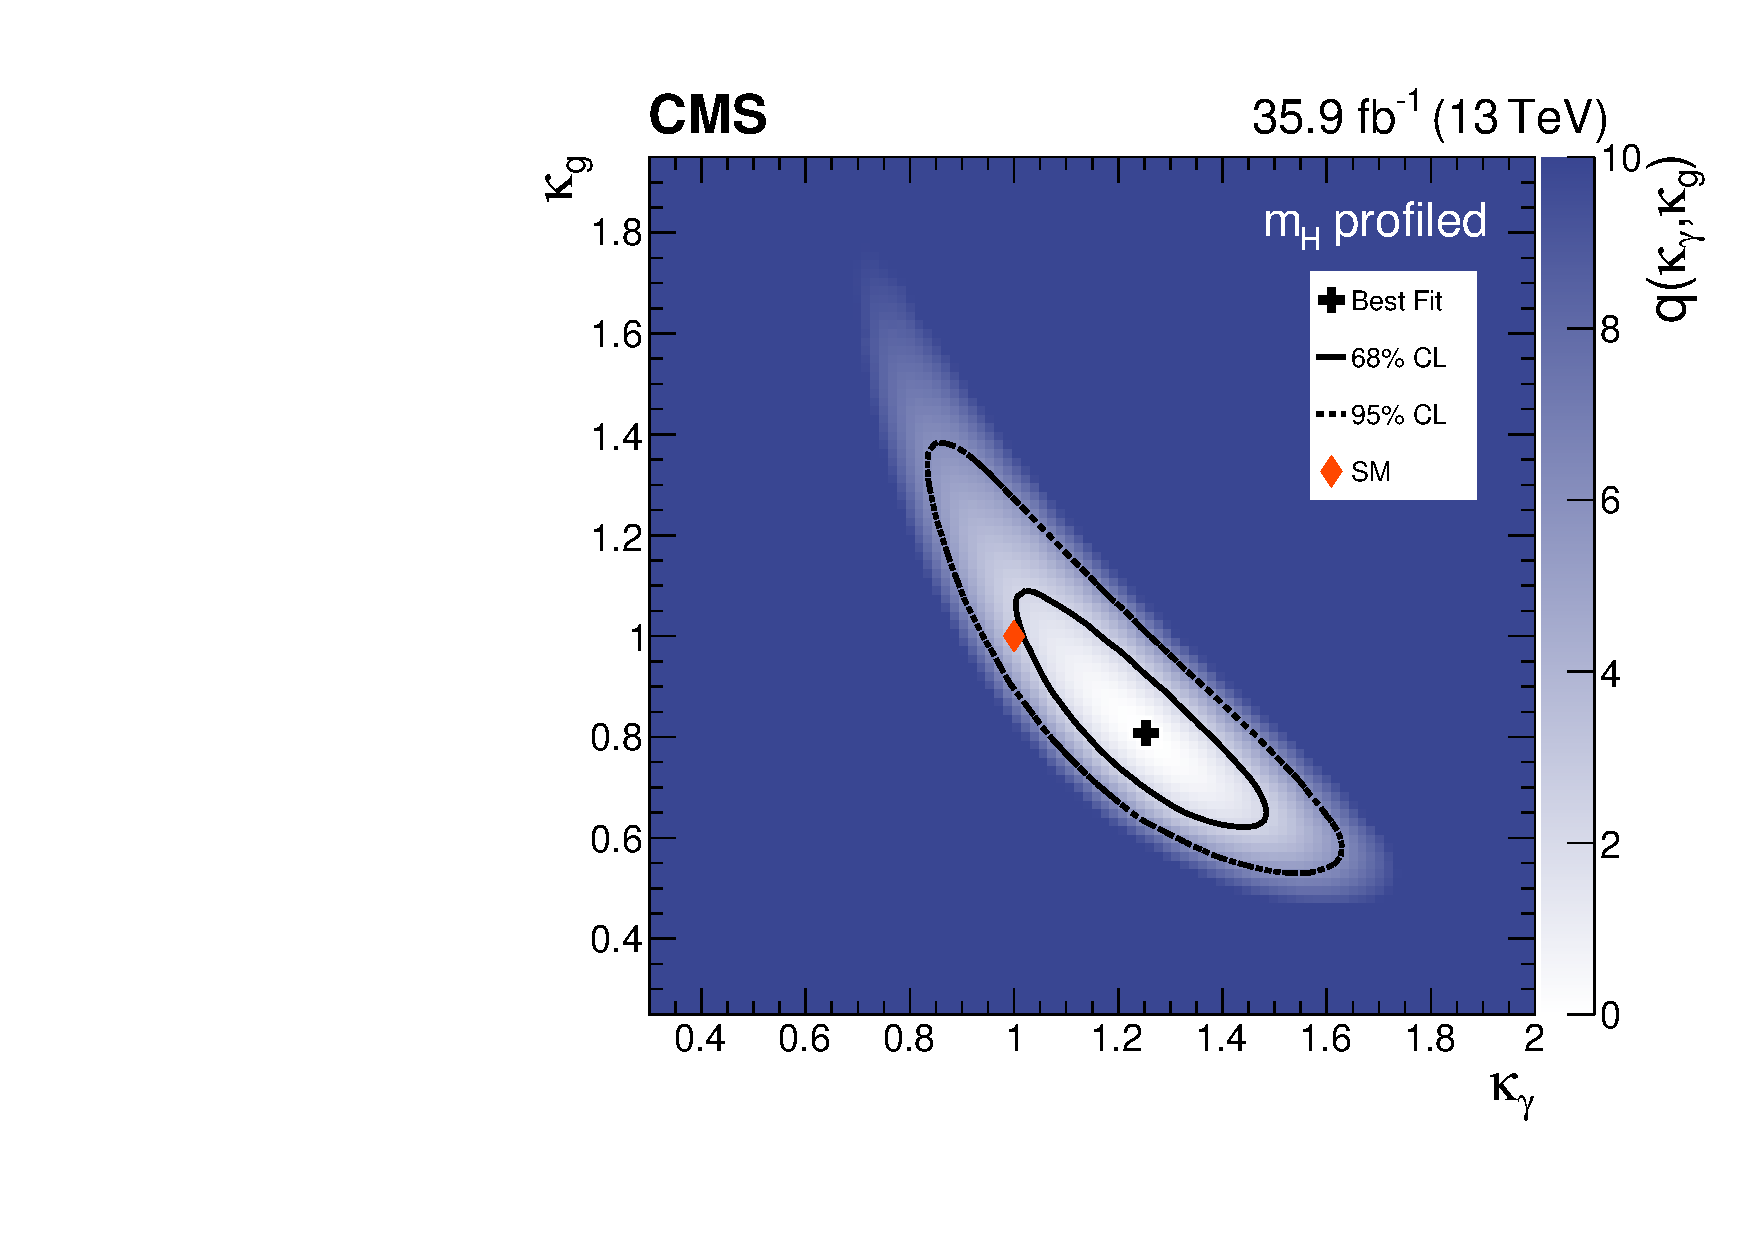
\includegraphics[width=0.49\textwidth]{figures/stats_results/CMS-HIG-16-040_Figure_020-b.pdf}
        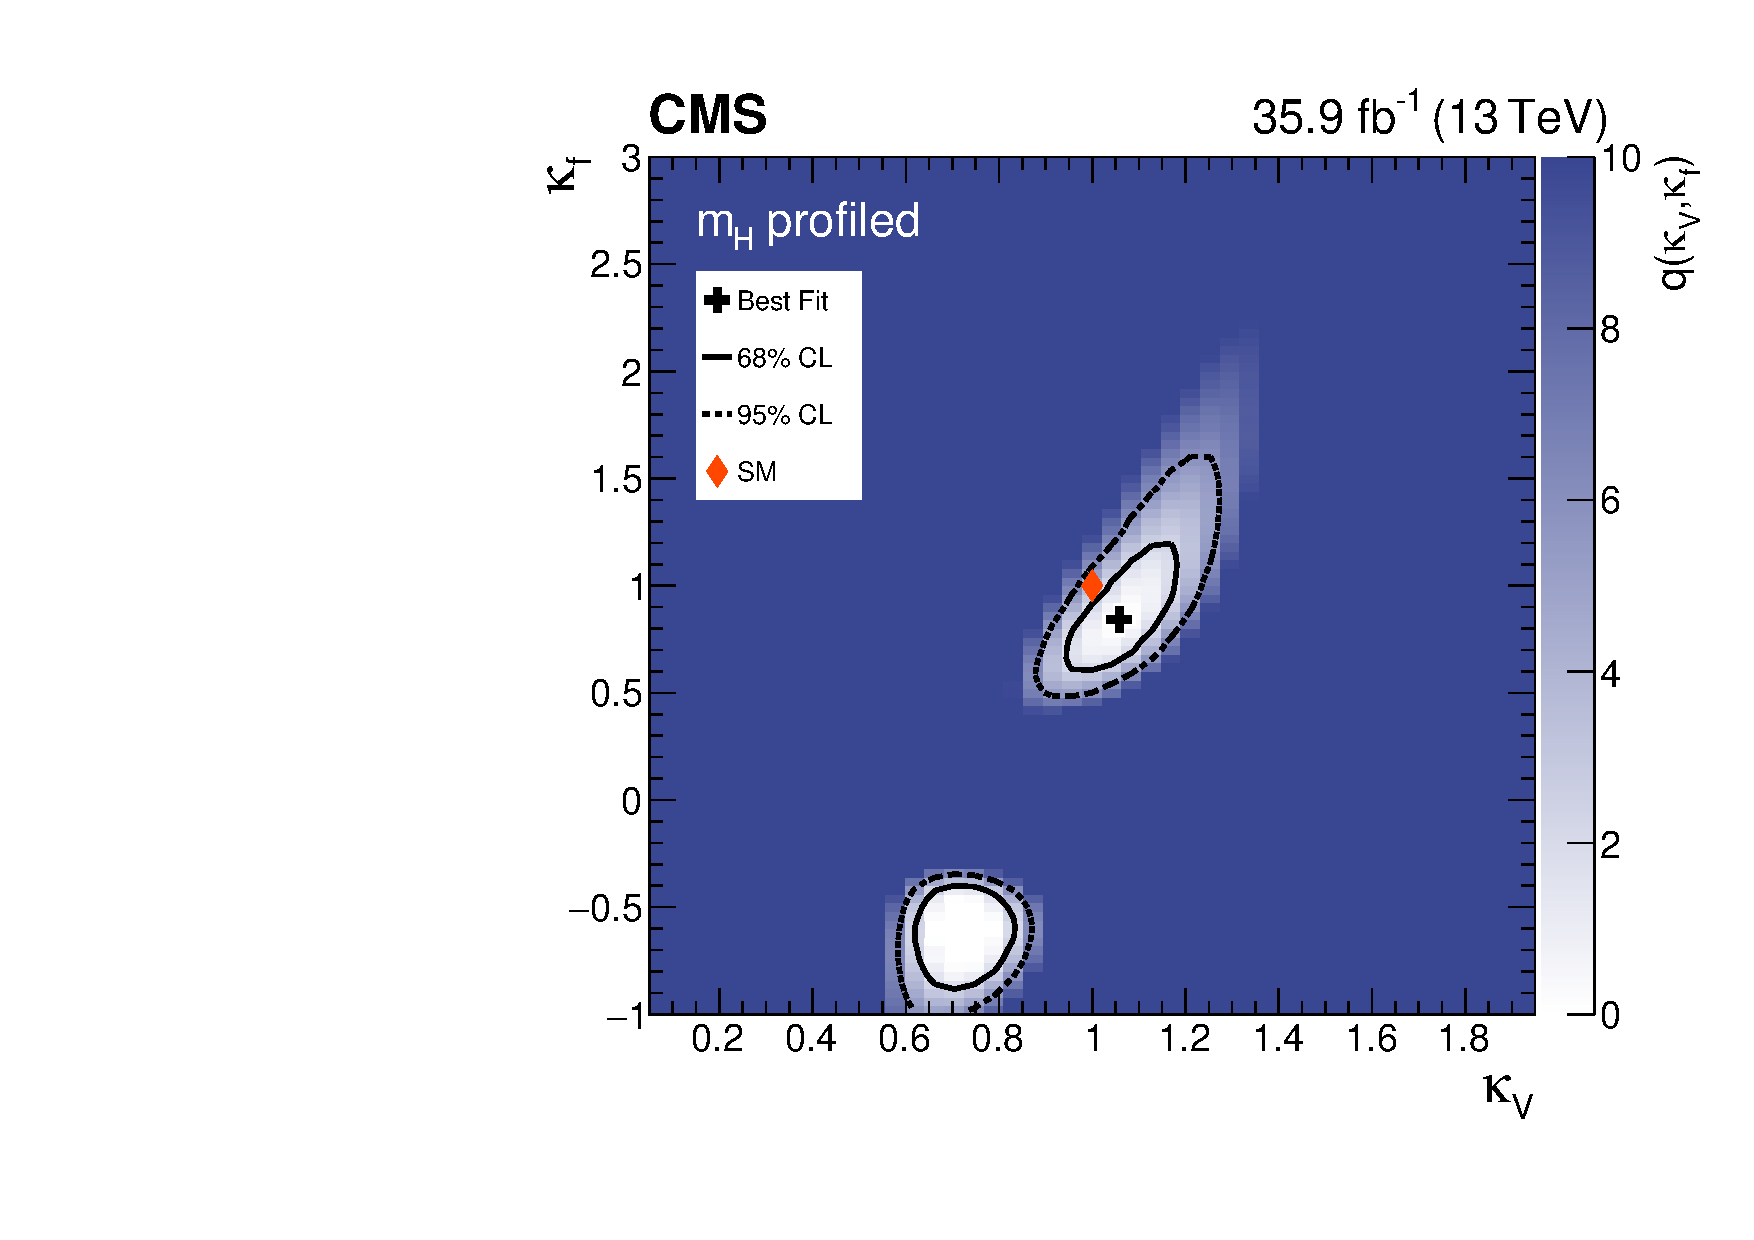
\includegraphics[width=0.49\textwidth]{figures/stats_results/CVCFScanProfileMH_col.pdf}
        \includegraphics[width=0.49\textwidth]{figures/stats_results/KGluKGamScanProfileMH_col.pdf}
    \end{center}
    \caption{Two-dimensional likelihood scan of $\kappa$ values for bosonic vs fermionic production modes (left) and effective gluon coupling versus effective photon coupling (right).
             The BDT-based VBF tag is shown on the top, and the DCNN-based tag is shown at the bottom.}
        \label{fig:stats_results:kappa}
\end{figure}

The DCNN-based case demonstrates a reduction in uncertainty in these measurements, especially for the couplings to bosons. 





\subsection{Conclusions}
A collection of measurements have been made comparing both the BDT-based and DCNN-based VBF tags. 
The initial best fit to all categories shows an increase in expected signal purity and significance in the VBF production mode.
In the likelihood scans the DCNN is seen to bring improvements to all of the measurements. 
The greatest impact is seen in measurements of the VBF signal strength modifier itself, and on measurements of the bosonic signal strength and coupling modifiers.
All measurements are compatible with the SM.






    \chapter{Conclusions}
\label{chap:conclusions}

\newpage
\section{Introduction}


\end{mainmatter}


\appendix
\begin{appendices}
    

\chapter{VBF Tag \Zee Validation Plots}
\label{appendix:vbf_zee}



\begin{figure}[h!]
    \begin{center}
        \includegraphics[width=0.45\textwidth]{figures/appendix_zee/lead_jet_eta_zee_LPS.pdf}
        \includegraphics[width=0.45\textwidth]{figures/appendix_zee/sublead_jet_eta_zee_LPS.pdf}
    \end{center}
    \caption{Jet pseudorapidity distributions for leading jet in $p_T$ (left) and subleading jet (right).}
\end{figure}

\begin{figure}[h!]
    \begin{center}
        \includegraphics[width=0.45\textwidth]{figures/appendix_zee/dijet_mass_zee_LPS.pdf}
        \includegraphics[width=0.45\textwidth]{figures/appendix_zee/delta_eta_zee_LPS.pdf}
    \end{center}
    \begin{center}
        \includegraphics[width=0.45\textwidth]{figures/appendix_zee/lead_jet_pt_zee_LPS.pdf}
        \includegraphics[width=0.45\textwidth]{figures/appendix_zee/sublead_jet_pt_zee_LPS.pdf}
    \end{center}
    \begin{center}
        \includegraphics[width=0.45\textwidth]{figures/appendix_zee/centrality_zee_LPS.pdf}
        \includegraphics[width=0.45\textwidth]{figures/appendix_zee/min_delta_r_jgam_zee_LPS.pdf}
    \end{center}
    \caption{Features}
\end{figure}

\begin{figure}[h!]
    \begin{center}
        \includegraphics[width=0.45\textwidth]{figures/appendix_zee/lead_ptom_zee_LPS.pdf}
        \includegraphics[width=0.45\textwidth]{figures/appendix_zee/sublead_ptom_zee_LPS.pdf}
    \end{center}
    \begin{center}
        \includegraphics[width=0.45\textwidth]{figures/appendix_zee/dphi_jetjet_zee_LPS.pdf}
        \includegraphics[width=0.45\textwidth]{figures/appendix_zee/dphi_gamgamjetjet_zee_LPS.pdf}
    \end{center}
    \begin{center}
        \includegraphics[width=0.45\textwidth]{figures/appendix_zee/dipho_bdt_zee_LPS.pdf}
        \includegraphics[width=0.45\textwidth]{figures/appendix_zee/total_ptom_zee_LPS.pdf}
    \end{center}
    \caption{More features}
\end{figure}



\end{appendices}


\begin{backmatter}
    

\end{backmatter}


\end{document}
